% Options for packages loaded elsewhere
\PassOptionsToPackage{unicode}{hyperref}
\PassOptionsToPackage{hyphens}{url}
%
\documentclass[
  12pt,
  openany]{book}
\usepackage{amsmath,amssymb}
\usepackage{iftex}
\ifPDFTeX
  \usepackage[T1]{fontenc}
  \usepackage[utf8]{inputenc}
  \usepackage{textcomp} % provide euro and other symbols
\else % if luatex or xetex
  \usepackage{unicode-math} % this also loads fontspec
  \defaultfontfeatures{Scale=MatchLowercase}
  \defaultfontfeatures[\rmfamily]{Ligatures=TeX,Scale=1}
\fi
\usepackage{lmodern}
\ifPDFTeX\else
  % xetex/luatex font selection
  \setmainfont[]{Times New Roman}
\fi
% Use upquote if available, for straight quotes in verbatim environments
\IfFileExists{upquote.sty}{\usepackage{upquote}}{}
\IfFileExists{microtype.sty}{% use microtype if available
  \usepackage[]{microtype}
  \UseMicrotypeSet[protrusion]{basicmath} % disable protrusion for tt fonts
}{}
\makeatletter
\@ifundefined{KOMAClassName}{% if non-KOMA class
  \IfFileExists{parskip.sty}{%
    \usepackage{parskip}
  }{% else
    \setlength{\parindent}{0pt}
    \setlength{\parskip}{6pt plus 2pt minus 1pt}}
}{% if KOMA class
  \KOMAoptions{parskip=half}}
\makeatother
\usepackage{xcolor}
\usepackage[left=2.54cm, right=2.54cm, top=2.54cm, bottom=2.54cm]{geometry}
\usepackage{color}
\usepackage{fancyvrb}
\newcommand{\VerbBar}{|}
\newcommand{\VERB}{\Verb[commandchars=\\\{\}]}
\DefineVerbatimEnvironment{Highlighting}{Verbatim}{commandchars=\\\{\}}
% Add ',fontsize=\small' for more characters per line
\usepackage{framed}
\definecolor{shadecolor}{RGB}{248,248,248}
\newenvironment{Shaded}{\begin{snugshade}}{\end{snugshade}}
\newcommand{\AlertTok}[1]{\textcolor[rgb]{0.94,0.16,0.16}{#1}}
\newcommand{\AnnotationTok}[1]{\textcolor[rgb]{0.56,0.35,0.01}{\textbf{\textit{#1}}}}
\newcommand{\AttributeTok}[1]{\textcolor[rgb]{0.13,0.29,0.53}{#1}}
\newcommand{\BaseNTok}[1]{\textcolor[rgb]{0.00,0.00,0.81}{#1}}
\newcommand{\BuiltInTok}[1]{#1}
\newcommand{\CharTok}[1]{\textcolor[rgb]{0.31,0.60,0.02}{#1}}
\newcommand{\CommentTok}[1]{\textcolor[rgb]{0.56,0.35,0.01}{\textit{#1}}}
\newcommand{\CommentVarTok}[1]{\textcolor[rgb]{0.56,0.35,0.01}{\textbf{\textit{#1}}}}
\newcommand{\ConstantTok}[1]{\textcolor[rgb]{0.56,0.35,0.01}{#1}}
\newcommand{\ControlFlowTok}[1]{\textcolor[rgb]{0.13,0.29,0.53}{\textbf{#1}}}
\newcommand{\DataTypeTok}[1]{\textcolor[rgb]{0.13,0.29,0.53}{#1}}
\newcommand{\DecValTok}[1]{\textcolor[rgb]{0.00,0.00,0.81}{#1}}
\newcommand{\DocumentationTok}[1]{\textcolor[rgb]{0.56,0.35,0.01}{\textbf{\textit{#1}}}}
\newcommand{\ErrorTok}[1]{\textcolor[rgb]{0.64,0.00,0.00}{\textbf{#1}}}
\newcommand{\ExtensionTok}[1]{#1}
\newcommand{\FloatTok}[1]{\textcolor[rgb]{0.00,0.00,0.81}{#1}}
\newcommand{\FunctionTok}[1]{\textcolor[rgb]{0.13,0.29,0.53}{\textbf{#1}}}
\newcommand{\ImportTok}[1]{#1}
\newcommand{\InformationTok}[1]{\textcolor[rgb]{0.56,0.35,0.01}{\textbf{\textit{#1}}}}
\newcommand{\KeywordTok}[1]{\textcolor[rgb]{0.13,0.29,0.53}{\textbf{#1}}}
\newcommand{\NormalTok}[1]{#1}
\newcommand{\OperatorTok}[1]{\textcolor[rgb]{0.81,0.36,0.00}{\textbf{#1}}}
\newcommand{\OtherTok}[1]{\textcolor[rgb]{0.56,0.35,0.01}{#1}}
\newcommand{\PreprocessorTok}[1]{\textcolor[rgb]{0.56,0.35,0.01}{\textit{#1}}}
\newcommand{\RegionMarkerTok}[1]{#1}
\newcommand{\SpecialCharTok}[1]{\textcolor[rgb]{0.81,0.36,0.00}{\textbf{#1}}}
\newcommand{\SpecialStringTok}[1]{\textcolor[rgb]{0.31,0.60,0.02}{#1}}
\newcommand{\StringTok}[1]{\textcolor[rgb]{0.31,0.60,0.02}{#1}}
\newcommand{\VariableTok}[1]{\textcolor[rgb]{0.00,0.00,0.00}{#1}}
\newcommand{\VerbatimStringTok}[1]{\textcolor[rgb]{0.31,0.60,0.02}{#1}}
\newcommand{\WarningTok}[1]{\textcolor[rgb]{0.56,0.35,0.01}{\textbf{\textit{#1}}}}
\usepackage{longtable,booktabs,array}
\usepackage{calc} % for calculating minipage widths
% Correct order of tables after \paragraph or \subparagraph
\usepackage{etoolbox}
\makeatletter
\patchcmd\longtable{\par}{\if@noskipsec\mbox{}\fi\par}{}{}
\makeatother
% Allow footnotes in longtable head/foot
\IfFileExists{footnotehyper.sty}{\usepackage{footnotehyper}}{\usepackage{footnote}}
\makesavenoteenv{longtable}
\usepackage{graphicx}
\makeatletter
\def\maxwidth{\ifdim\Gin@nat@width>\linewidth\linewidth\else\Gin@nat@width\fi}
\def\maxheight{\ifdim\Gin@nat@height>\textheight\textheight\else\Gin@nat@height\fi}
\makeatother
% Scale images if necessary, so that they will not overflow the page
% margins by default, and it is still possible to overwrite the defaults
% using explicit options in \includegraphics[width, height, ...]{}
\setkeys{Gin}{width=\maxwidth,height=\maxheight,keepaspectratio}
% Set default figure placement to htbp
\makeatletter
\def\fps@figure{htbp}
\makeatother
\setlength{\emergencystretch}{3em} % prevent overfull lines
\providecommand{\tightlist}{%
  \setlength{\itemsep}{0pt}\setlength{\parskip}{0pt}}
\setcounter{secnumdepth}{5}
\ifLuaTeX
\usepackage[bidi=basic]{babel}
\else
\usepackage[bidi=default]{babel}
\fi
\babelprovide[main,import]{spanish}
\ifPDFTeX
\else
\babelfont[spanish]{rm}{Times New Roman}
\fi
% get rid of language-specific shorthands (see #6817):
\let\LanguageShortHands\languageshorthands
\def\languageshorthands#1{}
\usepackage{booktabs}
\usepackage{longtable}
\usepackage[none]{hyphenat}
\raggedbottom
\usepackage{blindtext}
\usepackage{textcomp}


\usepackage{scrlayer-scrpage}
\usepackage{lipsum}% just to generate text for the example

\pagestyle{scrheadings}
\clearpairofpagestyles
\ohead{\rightmark}
\cfoot[\pagemark]{\pagemark}



\let\oldmaketitle\maketitle
\AtBeginDocument{\let\maketitle\relax}
\usepackage{booktabs}
\usepackage{longtable}
\usepackage{array}
\usepackage{multirow}
\usepackage{wrapfig}
\usepackage{float}
\usepackage{colortbl}
\usepackage{pdflscape}
\usepackage{tabu}
\usepackage{threeparttable}
\usepackage{threeparttablex}
\usepackage[normalem]{ulem}
\usepackage{makecell}
\usepackage{xcolor}
\usepackage{fontspec}
\usepackage{multicol}
\usepackage{hhline}
\newlength\Oldarrayrulewidth
\newlength\Oldtabcolsep
\usepackage{hyperref}
\ifLuaTeX
  \usepackage{selnolig}  % disable illegal ligatures
\fi
\usepackage[]{natbib}
\bibliographystyle{apalike}
\IfFileExists{bookmark.sty}{\usepackage{bookmark}}{\usepackage{hyperref}}
\IfFileExists{xurl.sty}{\usepackage{xurl}}{} % add URL line breaks if available
\urlstyle{same}
\hypersetup{
  pdftitle={RECUPERACIÓN, EXTRACCIÓN Y CLASIFICACIÓN DE INFORMACIÓN DE SABER UCV},
  pdfauthor={José Miguel Avendaño Infante},
  pdflang={es-ES},
  hidelinks,
  pdfcreator={LaTeX via pandoc}}

\title{RECUPERACIÓN, EXTRACCIÓN Y CLASIFICACIÓN DE INFORMACIÓN DE SABER UCV}
\usepackage{etoolbox}
\makeatletter
\providecommand{\subtitle}[1]{% add subtitle to \maketitle
  \apptocmd{\@title}{\par {\large #1 \par}}{}{}
}
\makeatother
\subtitle{Caso de Estudio Repositorio www.saber.ucv.ve}
\author{José Miguel Avendaño Infante}
\date{2023-12-02}

\begin{document}
\maketitle

%\vspace{-2.0cm}
\pagenumbering{roman}
\thispagestyle{empty}
\begin{center}
	UNIVERSIDAD CENTRAL DE VENEZUELA\\
	FACULTAD DE CIENCIAS\\
	POSTGRADO EN CIENCIAS DE LA COMPUTACI\'ON\\

	\begin{figure}
						\centering
						  
\includegraphics[height=.7\textwidth]{images/UCV.png}
  \end{figure}
  \vspace{1.5cm}
  \large{\textbf{RECUPERACI\'ON, EXTRACCI\'ON Y CLASIFICACI\'ON DE \\ INFORMACI\'ON DE SABER UCV}}

  \vspace{3cm}
  Trabajo de grado de Maestría presentado ante la \\
  ilustre Universidad Central de Venezuela por el\\
  Econ. José Miguel Avendaño Infante para  optar
  al título de \\Magister Scientiarum en Ciencias de la Computaci\'on\\
  \vspace{0.5cm}
  Tutor: Dr. Andres Sanoja\\
  \vspace{1.5cm}
  Caracas - Venezuela\\
  Octubre 2023
\end{center}


\newpage
\thispagestyle{empty}
\large{\textbf{Resumen:}}

Se presenta la investigación \emph{Recuperación, Extracción y Clasificación de Información de Saber UCV} donde se ejecutan procesos de clasificación, almacenamiento y recuperación de información sobre las tesis y trabajos de grado que se encuentran publicados en el repositorio institucional Saber UCV.

Se implementa un Sistema que permite clasificar los documentos mencionados, según el área académica donde cursó estudios el autor de la investigación.

Se extráen los resúmenes de los trabajos y con las clasificaciones obtenidas se conforma un corpus sobre el cual se genera un índice invertido. Al corpus se le aplican técnicas de Procesamiento de Lenguaje Natural, de Minería de Datos y con modelos preentrenados de inteligencia artificial se crean  \textit{embeddings} de textos. Con toda la información procesada se alimenta una base de datos indexada.

El Sistema adicionalmente cuenta con una aplicación web para hacer procesos de Recuperación de Información donde el usuario puede hacer la exploración del corpus, incluida la búsqueda semántica, indicando el: texto a buscar, rango de fechas, área en la cual se generó la investigación, el nivel académico; posteriormente se recuperan los trabajos de mayor relevancia, enriqueciendo la experiencia con la presentación de los resultados en tablas interactivas, Mapas de Conocimiento y recomendaciones de documentos que puedan ser de interés.

La aplicación se implementa bajo un sistema distribuido con la arquitectura cliente-servidor y se soporta en el uso de contenedores orquestados.

\vspace*{2cm}

\textbf{Palabras Clave::} Recuperación de Información, Corpus, Procesamiento del Lenguaje Natural, Relevancia, Inteligencia Artificial, Embeddings, Búsqueda Semántica, Mapas de Conocimiento.



\newpage
\thispagestyle{empty}
\large{\textbf{Abstract:}}

The research \emph{Recovery, Extraction and Classification of Information from Saber UCV} is presented, where processes of classification, storage and retrieval of information on theses and degree works published in the institutional repository Saber UCV are executed.

A system is implemented that allows classifying the mentioned documents, according to the academic area where the author of the research studied.

The abstracts of the works are extracted and with the obtained classifications a corpus is formed on which an inverted index is generated. Natural Language Processing and Data Mining techniques are applied to the corpus, and with pre-trained artificial intelligence models, text \textit{embeddings} are created. With all the processed information an indexed database is fed.

The system also has a web application for Information Retrieval processes where the user can explore the corpus, including the semantic search, indicating the: text to search, date range, area in which the research was generated, academic level; subsequently the most relevant works are retrieved, enriching the experience with the presentation of the results in interactive tables, Knowledge Maps and recommendations of documents that may be of interest.

The application is implemented under a distributed system with client-server architecture and is supported by the use of orchestrated containers.

\vspace*{2cm}

\textbf{Keywords:} Information Retrieval, Corpus, Natural Language Processing, Relevance,  Artificial Intelligence, Embeddings, Semantic Search, Knowledge Maps.

\thispagestyle{empty}


%\newpage


\setlength{\abovedisplayskip}{-5pt}
\setlength{\abovedisplayshortskip}{-5pt}
\thispagestyle{empty}

\newpage
\begin{center}
\large{\textbf{\emph{\Huge{Dedicatoria:}}}}
\end{center}
\thispagestyle{empty}
\vspace*{5cm}
\thispagestyle{empty}
\begin{center} \Large \emph{A mi hijo Cassiel y  } \end{center}
\vspace*{1cm}
\begin{center} \Large \emph{mi esposa Waleska.} \end{center}
\vspace*{1cm}
\begin{center} \Large {\emph{De ustedes es esta investigación.}} \end{center}



\newpage
\begin{center}
\large{\textbf{\emph{\Huge{Agradecimientos:}}}}
\end{center}
\thispagestyle{empty}
\vspace*{2cm}
\thispagestyle{empty}

- A mi madre, obvio, sino no habría ni una sola palabra acá.\\\\
- A mi padre Fernando por negarme el Atari e insistir en el Oddysey 2.\\\\
- A mi tía Mercedes Infante y mi tío Teófilo García \textdagger, por "lo que fue y será".\\\\
- A mi hermano David por su aguante y soporte.\\\\
- A mi primo Cesar Alejandro García por todo el soporte.\\\\
- Dr. Andres Sanoja primero por aceptar la tutoría y enseñarme qué es la investigación dentro de una comunidad científica.\\\\
- Dr. José Mirabal por siempre andar con alguna idea a desarrollar y el tiempo dedicado a escuchar las propuestas y complementar esta Investigación.\\\\
- Dra. Concettina Di Vasta por las imponentes sesiones de 2 horas 15 minutos llenas de coherencia y conocimiento.\\\\
- Dra. Haydemar Nuñez por la rigurosidad al impartir los conocimientos.\\\\
- Dra. Vanessa Leguizamo por tomarse el tiempo de revisar la solicitud de estudio de un oxidado economista y por ser mi Prof.ª.\\\\
- Dra. Mairene Colina por la ayuda y sugerencias a lo largo de la investigación.\\\\
- Dr. Roberto Abalde por haberme dejado entrar de oyente a su Diplomado y generar tanto interés en estos temas.\\\\
- Mauricio Sáez Toro del equipo Saber UCV por mantener activo el Sistema Saber UCV y disponer del tiempo para colaborar con esta investigación.\\\\
- A Alexandra Asanovna Elbakyan por ayudar a liberar el conocimiento.\\\\
- A todo el personal del Postgrado: sus buenos días, por tener a mano la llave, por ayudar a mantener viva la Academia.\\\\
- A toda la comunidad de creadores de software libre y open source, en especial a los \#useRs por motivarme a adentrarme al mundo de las ciencias de la computación.\\\\


\newpage
\thispagestyle{empty}
\vspace*{5cm}
\hfill
\begin{minipage}{0.70\textwidth}
\begin{quote}
Como todos los hombres de la Biblioteca, he viajado en mi juventud; he peregrinado en busca de un libro, acaso del \emph{catálogo de catálogos}; ahora que mis ojos caso no pueden descifrar lo que escribo, me preparo a morir a unas pocas leguas del hexágono en que nací.\\
--- Jorge Luis Borges, \textit{La Bibioloteca de Babel}, Ficciones
\end{quote}
\hspace*{2cm}

\begin{quote}
Every important aspect of programming arises somewhere in the context of sorting or searching.

--- Donald Knuth, \textit{The Art of Computer Programming}, Volume 3
\end{quote}
\end{minipage}

\thispagestyle{empty}
\maketitle



{
\setcounter{tocdepth}{4}
\tableofcontents
}
\listoffigures
\listoftables
\clearpage
\pagenumbering{arabic}

\hypertarget{introduccion}{%
\chapter{Introducción:}\label{introduccion}}

Es conocida la gran disponibilidad de información en distintos formatos que tienen a su disposición los investigadores. Ejemplo de esto son libros en las bibliotecas o la variedad de documentos que se encuentran accesibles en formatos digitales como artículos publicados en revistas arbitradas o investigaciones alojadas en repositorios digitales. Es en esta abundancia donde recaen varios de los problemas a los cuales se enfrenta la labor investigativa, en particular, cuando se realiza la fase exploratoria de selección de aquellos textos que puedan resultar de mayor importancia.

Una de las herramientas que tienen a su disposición los investigadores, para la búsqueda de información que se encuentra en formato digital, son los Sistemas de Recuperación de Información. En ellos, ante un texto que representa una necesidad, son recuperados los documentos que cumplen ciertos criterios y en la representación del resultado se deben jerarquizar los que poseen mayor relevancia \citep{manning2008}.

En el caso de la Universidad Central de Venezuela existe un repositorio digital de documentos académicos denominado Saber UCV al que se puede acceder desde la dirección web \href{http://saber.ucv.ve/}{saber.ucv.ve}. Dentro de él se cuenta con un sistema que permite realizar búsquedas sobre las investigaciones generadas en la comunidad universitaria.

En este Trabajo de Grado se presenta la propuesta para la \textbf{Recuperación, Extracción y Clasificación de Información de Saber UCV}, mediante el desarrollo de un sistema informático que se denomina \textbf{Sistema Complementario Saber UCV (SCSU)}.

La implementación del SCSU es de utilidad para los investigadores que necesitan encontrar información sobre el conjunto de: tesis doctorales, trabajos de grado de maestría, trabajos especiales de grado, trabajos de ascenso y trabajos de grado; al ofrecer una mayor cantidad de parametros que permiten refinar la búsqueda.

Las funcionalidades que incorpora el SCSU se sustentan en procesos de extracción y clasificación de datos que originalmente no se encuentran estructurados en el repositorio oficial, como el nombre de la carrera de pregrado o el postrgrado donde fue generada la investigación y el nombre del tutor correspondiente.

Igualmente se aplican métodos para el Procesamiento del Lenguaje Natural y Minería de Texto para representar ``Mapas de Conocimiento'' \citep{dueñas2011} y los resultados de la búsqueda son enriquecidos con recomendaciones de documentos similares.

Otra funcionalidad disponible en el SCSU es la ``búsqueda semántica'' la cual permite recuperar información relevante basada en el significado contextual y la relación semántica de los términos.

\hypertarget{estructura}{%
\section{Estructura:}\label{estructura}}

En el Capítulo \ref{capproblema} \textbf{El Problema} se hace una ``Descripción del Problema'' enfrentado, mientras que en \ref{delimitacion} se hace la ``Delimitación del Problema''. En \ref{justificacion} se expone la ``Justificación e Importancia'' de realizar este estudio y en \ref{descripcion} ``Descripción de la Solución'' se presenta la Solución junto con el \ref{objegeneral} ``Objetivo General'' y los \ref{objeespe} ``Objetivos Específicos''. En \ref{aporte} se enumeran los ``Aportes'' que hace esta investigación.

En el Capítulo \ref{teorico} \textbf{Marco Teórico} se hace una ``Reseña Histórica'' \ref{alghist} sobre el problema computacional que representa la ``búsqueda''. En la sección \ref{infret} ``Recuperación de Información'' se mencionan los conceptos claves para comprender los procesos de búsqueda de texto dentro de un Corpus y se introducen a los ``Sistemas de Recuperación de Información'' que permiten ejecutar dicha tarea. Luego en \ref{MRI} se describen algunos ``Modelos de Recuperación de Información'' que se usan en la implementación del SCSU. Para representar los resultados de las búsquedas, el Sistema implementado necesita que los textos sean procesados mediante diversos métodos que son descritos en \ref{PT} ``Procesamiento a los Textos''. Seguidamente en \ref{SD} se definen a los ``Sistemas Distribuidos'', motivado a que la implementación realizada se hace mediante este tipo de sistemas. Al finalizar este Capítulo en \ref{sota} se presentan el ``Estado del Arte'' en lo relativo a los procesos de Recuperación de Información.

En el Capítulo \ref{mm} \textbf{Marco Metodológico} se presenta la ``Metodología de Trabajo Kanban'' \ref{mmmetodologia} que sirvió para realizar la planificación de la investigación y el ``Desarrollo Adaptable de Software --Adaptive Software Development (ASD)''- \ref{mmasd} que fue la metodología adoptada para realizar los Ciclos de Desarrollo del SCSU.

En el Capítulo \ref{desarrollo} \textbf{Desarrollo de la Solución} se presenta la \ref{desarollodescripcion} ``Descripción General de la Solución''. En \ref{desarrolloarquitectura} se presenta la ``Arquitectura'' mientras que \ref{desarrollociclos} se muestran los ``Ciclos de Desarrollo'' y sus correspondientes iteraciones.

Para concluir esta investigación, en el Capítulo \ref{conclusiones} \textbf{Conclusiones} se exponen en \ref{conclusionescontri} las ``Contribuciones'' y en \ref{conclusionestrabafutu} los ``Trabajos Futuros''que se pueden derivar del proceso expuesto a lo largo del contenido de los capítulos anteriormente citados.

\hypertarget{capproblema}{%
\chapter{El Problema:}\label{capproblema}}

En el presente Capítulo en \ref{desproblema} se hace la \textbf{Descripción del Problema}. En \ref{delimitacion} se hace la \textbf{Delimitación del Problema}. En \ref{justificacion} \textbf{Justificación e Importancia} se mencionan la razones principales que motivan haber llevado a cabo esta investigación. En \ref{descripcion} \textbf{Descripción de la Solución} se hace una aproximación a la propuesta general.

En \ref{objegeneral} se menciona el \textbf{Objetivo Principal} que se trazó, mientras que en \ref{objeespe} se enumeran los \textbf{Objetivos Específicos} y en \ref{aporte} se listan los \textbf{Aportes} efectuados.

\hypertarget{desproblema}{%
\section{Descripción del Problema:}\label{desproblema}}

La Universidad Central de Venezuela cuenta con un repositorio digital de documentos que se llama Saber UCV donde se alojan distintas investigaciones realizadas por la comunidad de la Universidad. Ingresando a la dirección web \url{http://saber.ucv.ve/} se permite ``el acceso libre a la producción intelectual, materiales y recursos académicos elaborados en las áreas de docencia, investigación y difusión de la UCV''. ¿Qué es Saber UCV?. (2023). Saber UCV. \href{http://saber.ucv.ve/}{http://saber.ucv.ve}.

Los usuarios interesados en hacer búsquedas sobre la información académica alojada en el repositorio, pueden efectuarlas introduciendo un texto y aplicando filtros sobre distintas categorías como:

\begin{itemize}
\item
  Seleccionar ``comunidades'': artículos de investigación, tesis (doctorales, maestrías, otras y pregrado), guías de estudio, revistas entre otras categorías.
\item
  Seleccionar la ``fecha de inicio'' referente al año en que se efectuó la publicación.
\end{itemize}

Igualmente pueden realizar la búsqueda sobre atributos específicos como el título del documento, el nombre del autor o el texto del resumen.

Dadas estas funcionalidades, en algunos casos el investigador que acuda a este repositorio puede necesitar filtrar información por el criterio del área académica donde fue realizada la investigación, no siendo esto posible al no contar los criterios ``nombre de facultad'' y ``nombre de escuela-postgrado''.

\hypertarget{delimitacion}{%
\section{Delimitación del Problema:}\label{delimitacion}}

El corpus con el que se trabajará es el subconjunto de los trabajos de grado de pregrado, trabajos especiales de grado de especialización, trabajos de grado de maestría, tesis doctorales y trabajos de ascenso, no abarcando otro tipo de documentos que se encuentran registrados en el repositorio.

No obstante en la implementación del ciclo de desarrollo \ref{desarrollociclos4} se incluyen dos revistas publicadas por la Universidad Central de Venezuela que son Gestión I+D y Episteme y una publicación del repositorio Saber U.L.A. de la Universidad de los Andes, para mostrar posibles ampliaciones en la ingesta de distintos tipos de publicaciones y fuentes dentro del SCSU.

Estas posibles incorporaciones implican procesos de revisión en las estructuras de los datos, ya que por los momentos el Sistema no está diseñado para automatizar tales procesos, sin la modificación de los códigos con los que se extrae la información desde los sitios web donde se alojan los documentos.

\hypertarget{descripcion}{%
\section{Descripción de la Solución:}\label{descripcion}}

La Solución que se propone es la implementación de un Sistema de Recuperación de Información con diversos componentes. Inicialmente de los trabajos mencionados en \ref{delimitacion}, mediante técnicas de extracción de nodos de archivos HTML´s, se obtienen de Saber UCV los siguientes datos de cada investigación: el título, el nombre del autor, las palabras claves, la fecha de publicación, el resumen y el enlace de descarga del documento que soporta el trabajo de grado.

Posteriormente el Sistema descarga el documento anexo a cada investigación, da lectura y clasifica la información del nombre de la facultad, la escuela o postgrado donde fue realizado el trabajo e igualmente extrae el nombre del tutor.

Todos los datos obtenidos son sometidos a técnicas del estado del arte en el Procesamiento del Lenguaje Natural y la Minería de Texto para conformar un corpus anotado, un índice invertido y se generan los vectores de \emph{embeddings} de texto. Posteriormente las tablas obtenidas se almacenan en una base de datos indexada.

El Sistema cuenta con una aplicación web que permite a los usuarios desde un navegador, explorar extensivamente el corpus anotado, realizando consultas de texto y aplicando varios filtros como la selección de la jerarquía, el área académica y el rango de fechas. La relevancia de los resultados recuperados se determina mediante una función de ponderación y los documentos se presentan de manera priorizada para mejorar la experiencia del usuario.

Adicionalmente, el Sistema ofrece recomendaciones de documentos que presentan similitud con aquellos que fueron recuperados en el proceso anterior. También representa los ``Mapas de Conocimiento'', según una adaptación \emph{ad-hoc} hecha para la implementación del SCSU basada en el trabajo de \citep{dueñas2011}, en una representación gráfica interactiva.

La solución implementada cuenta con procesos automatizados de actualización para incorporar las nuevas investigaciones que sean añadidas al repositorio Saber UCV y se soporta en un sistema distribuido conformado por contenedores que son gestionados por un orquestador con la arquitectura ``modelo-vista-controlador''.

En la figura \ref{fig:arquitecturasri} se muestra un diagrama con la arquitectura del SCSU. (falta adaptarlo-pequeños cambios).

\begin{figure}

{\centering 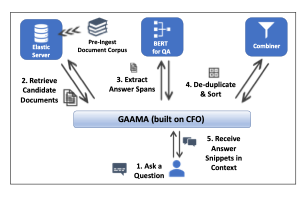
\includegraphics[width=0.6\linewidth]{images/02-problema/arquitectura_sri} 

}

\caption{Arquitectura del Sistema-Este diagrama se va a traducir y adaptar al SCSU. Se coloca ya que es muy similar a la Solución Implementada}\label{fig:arquitecturasri}
\end{figure}

\hypertarget{justificacion}{%
\section{Justificación e Importancia:}\label{justificacion}}

Con esta Investigación se implementa un método que permite subsanar la falta de clasificaciones por áreas académica que tiene el repositorio Saber UCV y mediante la aplicación web se amplían los criterios de búsqueda disponibles para investigadores que necesiten realizar consultas sobre los documentos disponibles en el repositorio.

\hypertarget{objegeneral}{%
\subsection{Objetivo General:}\label{objegeneral}}

Implementar un Sistema en el que se puedan realizar procesos de recuperación de información (\emph{information retrieval}), extracción y clasificación de los textos académicos alojados en el Repositorio Saber UCV, empleando técnicas de procesamiento de lenguaje natural, de minería de texto y usando modelos de lenguaje preentrenados de inteligencia artificial.

\hypertarget{objeespe}{%
\subsection{Objetivos Específicos:}\label{objeespe}}

\begin{enumerate}
\def\labelenumi{\arabic{enumi}.}
\item
  Conformar un corpus con los resúmenes, títulos, palabras claves y nombres de autor con todos los documentos de tesis doctorales y trabajos de grado de pregrado y maestría alojados en Saber UCV.
\item
  Clasificar los trabajos de grado alojados en Saber UCV por área académica donde se haya realizado la investigación y extraer el nombre completo del tutor. (nota para el Prof.~Mirabal: en este punto se puede separar, o colocar un nombre genérico para el objetivo como: creación de metadata a partir del texto contenido en los documentos de cada trabajo de grado).
\item
  Crear una aplicación web con una interface de navegación de corpus que facilite realizar ``búsquedas de texto completo'' o ``búsqueda semántica'' con acceso a información de relevancia que permita generar ``Mapas de Conocimiento''.
\item
  Generar recomendaciones de investigaciones que presenten similitud con los documentos recuperados por el Sistema.
\end{enumerate}

\hypertarget{aporte}{%
\section{Aportes:}\label{aporte}}

Algunos de los aportes que se generaron al realizar esta investigación son los siguientes:

\begin{itemize}
\item
  Se mejora y flexibilizan los criterios de búsqueda en comparación a los que tiene el repositorio Saber UCV al clasificar por área académica un total de 9.585 investigaciones de 9.982 potenciales documentos a categorizar.
\item
  Se crea un listado con 425 categorías de carreras de pregrado, especializaciones, maestrías y doctorados que se imparten en la Universidad.
\item
  Se obtiene un listado de potenciales tutores de las investigaciones realizadas con 8.217 nombres y una cantidad de 3.766 nombres únicos.
\item
  Se crean visualizaciones y representaciones de ``Mapas de Conocimiento''.
\item
  Se implementa la búsqueda de texto completo con una función de relevancia distinta a la de Saber UCV permitiendo obtener mejores métricas de desempeño en la tarea de ``recuperación de información''
\item
  Se implementa un ``sistema de recomendación'' de documentos que presenten similitudes con los textos recuperados.
\item
  La experiencia del usuario se enriquece mediante gráficos que muestran la evolución de aparición de los términos buscados en el período establecido para la recuperación de información.
\item
  Todos los componentes del Sistema son de código abierto, libres de algún pago de licencia.
\item
  La implementación se hace mediante un orquestador de contenedores, teniendo asociados los archivos ``docker compose'' y ``dockerfiles'', que facilitan que pueda estar en producción el Sistema con un mínimo de configuraciones y se garantiza la reproducibilidad de los códigos que conforman la Solución.
\item
  La propuesta es escalable y adaptable a la demanda de accesos.
\item
  El Sistema está diseñado para poder actualizar los datos registrados con la periodicidad que se defina.
\item
  El Sistema puede servir de prototipo para integrar publicaciones de otros repositorios de documentos que pertenecen a instituciones nacionales de investigación.
\item
  Se realiza la implementación de ``búsquedas semánticas''.
\end{itemize}

\hypertarget{teorico}{%
\chapter{Marco Teórico-Referencial:}\label{teorico}}

En este capítulo se exponen los fundamentos teóricos en que se sustentan los procesos y métodos aplicados en la investigación \textbf{Recuperación, Extracción y Clasificación de Información de SABER UCV}.

En \ref{alghist} se hace una \textbf{Reseña histórica} sobre los procesos de búsqueda, en \ref{infret} se examina qué es la \textbf{Recuperación de Información} (RI), en \ref{SRI} se indica qué son los \textbf{Sistemas de Recuperación de Información (SRI}) y en \ref{ejemplos-de-irs} se muestran un par de ejemplos de SRI. Adicionalmente en \ref{MRI} \textbf{Modelos de Recuperación de Información} se exploran modelos como el \ref{MRIbol} \textbf{Boleano} y el \ref{invind} de \textbf{Índices Invertidos}. En la sección \ref{relevancia} se introduce el concepto de \textbf{Relevancia} que es clave para comprender cuál es uno de los principales objetivos que tiene cualquier SRI. En \ref{ranking} \textbf{Re Ordenamiento} se exponen dos algoritmos usados para jerarquizar los documentos que sean más relevantes en un proceso de RI y en \ref{evaluacion} \textbf{Métodos de Evaluación} se muestran algunas técnicas usadas para medir la precisión que se obtiene en los procesos de recuperación de información.

Para indicar los métodos con los que es tratado el Corpus de esta Investigación en \ref{PT} \textbf{Procesamiento de Texto} se muestran las técnicas del \ref{nlproc} \textbf{Procesamiento de Lenguaje Natura}l y de \ref{textmin} \textbf{Minería de Texto}. En \ref{similitud} \textbf{Similitud de Documentos} se indica cómo se puede comparar la similitud de los textos y su aplicación.

Adicionalmente, al formar parte de este Investigación, el desarrollo e implementación del software denominado \textbf{Sistema Complementario Saber UCV (SCSU)}, se exponen definiciones asociadas a los \ref{SD} \textbf{Sistemas Distribuidos}, sentando las bases para el desarrollo e implementación del \textbf{SCSU}.

Se finaliza este Capítulo haciendo una inspección en \ref{sota} a lo que constituye el \textbf{Estado del Arte} en la materia, haciendo énfasis en la representación de textos mediante \ref{embed} \textbf{Embeddings}, en \ref{trans} se introduce la \textbf{Arquitectura de} \textbf{Redes Neuronales Transformers} con que se logran generar los embeddings de mayor calidad para el IR y brevemente se muestra en \ref{LLM} los \textbf{Largos Modelos de Lenguaje (LLM´s)}, mientras en \ref{int} \textbf{Integración} se comentan los distintos avances y tendencias que se presentan en los Sistemas de Recuperación de Información.

\hypertarget{alghist}{%
\section{Reseña histórica:}\label{alghist}}

El profesor Donald Knuth señala, dentro del campo de las ciencias de la computación, que la \textbf{búsqueda} \emph{es el proceso de recolectar información que se encuentra en la memoria del computador de la forma más rápida posible, esto cuando tenemos una cantidad N de registros y nuestro problema es encontrar el registro apropiado de acuerdo a un criterio de búsqueda} \citep[p.392]{knuth1997} .Iniciamos con esta cita porque la recuperación de información gira en torno a un problema central de las ciencias de la computación que es la \textbf{búsqueda}.

En la década de 1940 cuando aparecieron las computadoras, las búsquedas no representaban mayor problema debido a que estas máquinas disponían de poca memoria \emph{RAM} pudiendo almacenar sólo moderadas cantidades de datos.

No obstante con el desarrollo e incremento del almacenamiento en memoria \emph{RAM} o en dispositivos de almacenamiento permanentemente, ya en la década de 1950 empezaron a aparecer los problemas de \textbf{búsqueda} y los primeras investigaciones para afrontarla.

En la década de 1960 se adoptan estrategias basadas en arboles. Los primeros algoritmos que sirvieron para localizar la aparición de una frase dentro de un texto, o expresado de forma más abstracta, como la detección de una subcadena \emph{P} dentro de otra cadena \emph{T}, fueron los algoritmos de ``\emph{Pattern-Matching}'' \citep{goodrich2013}.

Así nos encontramos en la literatura con el algoritmo ``Fuerza Bruta'' donde dado un texto T y una subcadena P, se va recorriendo cada elemento de la cadena T para detectar la aparición de la subcadena P. Si bien este algoritmo no presentaba el mejor desempeño, creó una forma válida de enfrentar el problema de la búsqueda de subcadenas de texto.

El algoritmo ``\emph{Knuth-Morris-Pratt''} que se introdujo en 1976 tenía como novedad que se agregó una función que iba almacenando''previas coincidencias parciales'' en lo que eran fallos previos y así al realizar un desplazamiento tomaba en cuenta cuántos caracteres se podían reusar. De esta forma se logró considerablemente mejorar el rendimiento en los tiempos de ejecución de \textbackslash( O\^{}\{(a+b)\} \textbackslash) que son asintóticamente óptimos.

Posteriormente en 1977 el problema se enfrenta con un nuevo algoritmo que es el de \emph{Boyer-Moore} en el cual se implementan dos heurísticas (\emph{looking-glass y} \emph{character-Jump)} que permiten ir realizando algunos saltos en la búsqueda, ante la no coincidencia de la subcadena con la cadena y adicionalmente, el orden en el que se va realizando la comparación se invierte. Estas modificaciones permitieron obtener un mejor desempeño.

Sobre una modificación al algoritmo \emph{Boyer-Moore} se sustenta la utilidad \emph{grep} de la línea de comandos UNIX que también da soporte a diversos lenguajes que la usan para ejecutar búsquedas de texto, con un proceso que comúnmente es conocido como \emph{grepping}. Esta utilidad fue ampliamente usada para resolver parcialmente lo que se expondrá en \ref{desarrollociclos1}.

Otra de las estrategias que surgió para enfrentar las búsquedas de texto, fue el uso de la programación lineal, donde bajo la premisa ``\emph{divida et impera'',} los problemas que requieren tiempo exponencial para ser resueltos son descompuestos en polinomios y por lo tanto se disminuye la complejidad en tiempo para encontrar la solución.

Entre este tipo de algoritmos se puede mencionar los de \emph{alineación de cadenas del ADN} de forma parcial o total dentro de una cadena mayor, siendo una versión de estos el algoritmo \textbf{\emph{Smith-Waterman}} \citep{smith1981}. Posteriormente se identificó que este tipo de solución era extrapolable a las subcadenas de texto. Un algoritmo que se usó para resolver el problema de hacer coincidir una etiqueta de clasificación con los textos del \emph{Corpus} en \ref{desarrollociclos1} fue el algoritmo precitado.

Un gran paso para aproximarnos a la aparición de los Sistemas de Recuperación de Información \ref{SRI} lo representó el enfoque que presentan los algoritmos \emph{Tries}. Este nombre proviene del proceso de \emph{Information Retrieval} y principalmente se basa en hacer una serie de preprocesamientos a los textos para que al momento de ejecutar la búsqueda de texto, es decir, de la subcadena dentro de la cadena, ya tengamos una parte del trabajo realizado previamente y no tener que ejecutarlo todo \emph{``on the fly''}, es decir, sobre la marcha.

Un \emph{Trie} \citep{fredkin1960} es una estructura de datos que se crea para almacenar textos para así poder ejecutar más rápido la coincidencia en la búsqueda. En la propuesta del \textbf{SCSU} todos los textos van siendo preprocesados con distintas técnicas a medida que son insertados en la base de datos.

\hypertarget{infret}{%
\section{Recuperación de Información:}\label{infret}}

El eje central sobre el cual gira el proceso de recuperación de información (RI) es satisfacer las necesidades de información relevante que sean expresadas por un usuario mediante una consulta de texto, lo que también se denomina el \textbf{\emph{query}}. El investigador Charu Aggarwal en su libro sobre Minería de Texto \citep{miningt2012} menciona que el objetivo del proceso de RI es conectar la información correcta, con los usuarios correctos en el momento correcto, mientras que otro de los autores con mayor dominio sobre el tema, Christopher Manning en su libro \emph{Information Retrieval} indica que ``es el proceso de encontrar materiales (generalmente documentos) de una naturaleza no estructurada (generalmente texto) que satisface una necesidad de información dentro de grandes colecciones (normalmente almacenada en computadores)'' \citep{manning2008}.

A los efectos de delimitar el espacio de búsqueda sobre el que se realiza la acción de la consulta, se define al \textbf{Corpus} como el conjunto cerrado de documentos codificados electrónicamente que se encuentra integrado en un sistema de almacenamiento \citep{martiaurora} o entendido desde otra perspectiva, es el conjunto de datos sobre el cuál se hará la búsqueda generando el proceso de recuperación de información.

Satisfacer una necesidad de recuperación de información no sólo se circunscribe a un problema búsqueda de un texto dentro de un \emph{corpus}. En la mayoría de los casos se deberá cumplir con ciertos criterios, o restricciones, como por ejemplo que el \emph{query} esté dentro de un período de fechas, o que se encuentre limitado a ciertas restricciones, siendo esto a lo que se le denomina ``búsqueda múlti atributo''.

La información que se recolecte en una búsqueda y el orden en que sea presentado el resultado al usuario, dependerá de varios factores como: la aparición, parcial o total, de las palabras del query en el documento; se puede dar un mayor peso a la aparición de la frase del \emph{query} dentro del título o palabras claves; la proximidad (la cercanía entre dos palabras) dentro del documento con las que se introducen en el \emph{query}; o por la frecuencia de aparición de una palabra, o varias, dentro del documento. En \ref{relevancia} \textbf{Relevancia} se darán más detalles sobre este particular.

Igual puede aportar un peso mayor a la recuperación de un documento, las referencias (citas) que contengan otros documentos a ese determinado escrito, similar a la propuesta del algoritmo \textbf{\emph{PageRank}} \citep{brin1998}, siendo el fin último, la extracción de los documentos que resulten de mayor relevancia para el usuario. Esta aproximación también puede usarse para la detección de comunidades dentro del \emph{Corpus} \citep{heydari2020analysis}.

Incluso es válido incorporar documentos, en los resultados que arroje la búsqueda, que propiamente no coincidan exactamente con los términos buscados sino que contengan palabras que sean sinónimos o que presenten alguna similitud con el texto del \emph{query}. Lo que acabamos de mencionar incorporará formalmente dentro del proceso de extracción de información algo de imprecisión con la intención última de enriquecer el proceso de \textbf{\emph{Information Retrieval}} \citep{kraft2017}. En \ref{similitud} \textbf{Similitud de Documentos} y en \ref{embed} \textbf{Embeddings,} se mencionan y especifican algunas de las técnicas con las cuales se incorporan este lote de documentos en los resultados de una búsqueda.

Evaluando el proceso con cierto nivel de abstracción se tiene que el proceso de recuperación de información está compuesto principalmente:

\begin{itemize}
\item
  por un \emph{query}
\item
  por un corpus y
\item
  por una función de \emph{ranking} \ref{ranking} para ordenar los documentos recuperados de mayor importancia a menor.
\end{itemize}

El desarrollo de los algoritmos expuestos en \ref{alghist}, sumado a la necesidad de resolver los problemas asociados a la búsqueda de un texto dentro de un \emph{corpus} con múltiples atributos, en tiempos aceptables y el crecimiento exponencial de datos disponibles en formato digital \citep{worldde2016}, potenciada por el uso generalizado de los computadores desde la década de 1980, abonó las condiciones para la creación de los \textbf{Sistemas de Recuperación de Información}.

\hypertarget{SRI}{%
\subsection{Sistemas de Recuperación de Información (SRI) :}\label{SRI}}

Los Sistemas de Recuperación de Información (\emph{Information Retrieval Systems-IRS}) son los dispositivos (software y/o hardware) que median entre un potencial usuario que requiere información y la colección de documentos que puede contener la información solicitada \citep{kraft2017} 1. El SRI se encargará de la representación, el almacenamiento y el acceso a los datos que estén estructurados y se tendrá presente que las búsquedas que sobre él recaigan tendrán distintos costos, siendo uno de estos el tiempo que tarde en efectuarse.

Es de nuestro conocimiento que generalmente los datos estructurados son gestionados mediante un sistema de base de datos, pero en el caso de los textos, estos se gestionan por medio de un motor de búsqueda, motivado a que los textos en un estado crudo carecen de estructura \citep{miningt2012} . Son los motores de búsqueda (\emph{search engines}) los que permiten que un usuario pueda encontrar fácilmente la información que resulte de utilidad mediante un \emph{query}.

El \textbf{SCSU} está diseñado como un SRI donde se pueden ejecutar querys, que son procesados y los resultados que se obtienen, son sometidos a una función de \emph{ranking} que será expuesta en una fase posterior del desarrollo de esta investigación.

\hypertarget{ejemplos-de-irs}{%
\subsection{Ejemplos de IRS:}\label{ejemplos-de-irs}}

Profundizando en el tema de esta Investigación se mencionan un par de páginas de internet que funcionan coomo IRS sobre corpus de investigaciones científicas.

\begin{enumerate}
\def\labelenumi{\arabic{enumi}.}
\item
  Arvix alojado en \url{https://arxiv.org/}, que es un repositorio de trabajos de investigación. Al momento del usuario hacer un requerimiento de información, adicional al texto de la búsqueda, se pueden indicar distintos filtros a aplicar como puede ser el área del conocimiento (física, matemática, computación, etc.), si se quiere buscar sólo dentro del título de una investigación, o el nombre autor, en el \emph{abstract, o} en las referencias.
\item
  Portal de la \emph{Asociation Computery Machine} (ACM) alojado en \url{https://dl.acm.org} incorpora un motor de búsqueda con particulares características ya que los resultados son acompañado por distintas representaciones gráficas que le dan un valor agregado. En la figura \ref{fig:busquedasacm} se ve una de estas representaciones que incluye la frecuencia de aparición del \emph{query} en el tiempo.
\end{enumerate}

\begin{figure}

{\centering 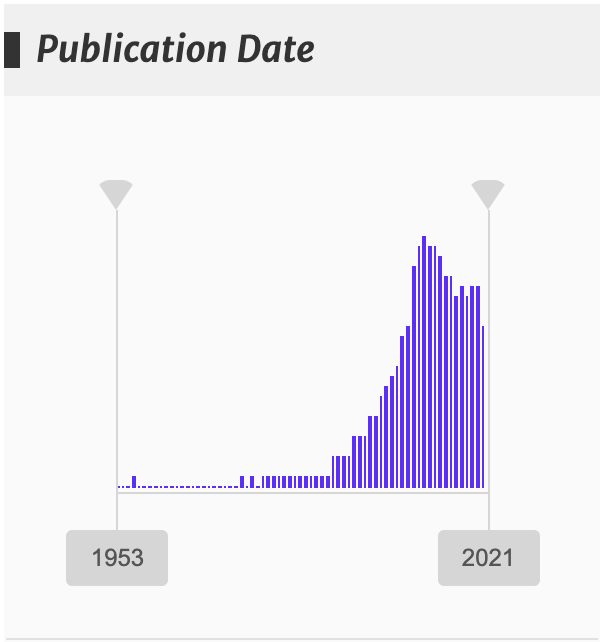
\includegraphics[width=0.3\linewidth]{images/03-marco-teorico/busquedaacm} 

}

\caption{Gráfico que acompaña resultados de búsqueda de un término en la biblioteca digital de la Association for Computing Machinery (https://dl.acm.org/)}\label{fig:busquedasacm}
\end{figure}

\hypertarget{MRI}{%
\subsection{Modelos de Recuperación de Información:}\label{MRI}}

\hypertarget{MRIbol}{%
\subsubsection{Recuperación boleana:}\label{MRIbol}}

Ante una búsqueda de información se recorre linealmente todo el documento para retornar un valor boleano indicando la presencia o no del término buscado. Es uno de los primeros modelos que se uso y está asociado a técnicas de \emph{grepping} \citep{manning2008}. El desarrollo de este modelo apareció entre 1960 y 1970.

El usuario final obtendrá como respuesta a su \emph{query} sólo aquellos textos que contengan el término. Es un modelo muy cercano a los típicos \emph{querys} de bases de datos con el uso de operadores ``AND'', ``OR'' y ``NOT''. En el procesamiento de los textos se genera una matriz de incidencia binaria término-documento, donde cada término que conforma el vocabulario, ocupa una fila \emph{i} de la matriz mientras que cada columna \emph{j} se asocia a un documento. La presencia de el término \emph{i} en el documento \emph{j} se denotará con un valor verdadero o un ``1''.

La recuperación boleana si bien representa una buena aproximación a la generación de \emph{querys} más rápidos, presenta una gran desventaja y es que al crecer la cantidad de documentos y el vocabulario (palabras únicas contenidas dentro del Corpus), se obtiene una matriz dispersa de una alta dimensionalidad que hace poco efectiva su implementación.

Los documentos y los \emph{querys} son vistos como conjuntos de términos indexados, que luego fueron llamados ``bolsa de términos'' \emph{(bag of terms)}. Las deficiencias de este modelo recaen en que los resultados, no tienen ningún ranking. Si por ejemplo el término sobre el cual se realiza el \emph{query} aparece 100 veces en un documento y en otro aparece sólo una vez, en la presentación de los resultados ambos documentos aparecerán al mismo nivel, no pudiendo mostrar preferencia del uno sobre el otro.

Otra de las desventajas es que no se registra el contexto semántico de las palabras e incluso se pierde el orden en que aparecen las palabras en cada texto.

Este modelo se presume que es el cual se basa la implementación de Saber UCV y por eso es que en general, se termina presentando el problema de que al usar el operador OR en las búsquedas exactas, se obtiene un gran \textbf{\emph{recall}} \footnote{Precision: la fracción, o porcentaje, de los documentos recuperados que son relevantes en la búsqueda efectuada. Recall, también denominado es español como ``exhaustividad'' mide la fracción de documentos relevantes que fueron recuperados con respecto a la totalidad de los documentos relevantes presentes en la base de datos.} en los resultados.

Con la propuesta del \ref{desarrollociclos3} Prototipo de Buscador del \textbf{SCSU} se obtiene una versión de recuperación de información que aplica métodos de mayor eficiencia y genera una mayor \emph{``precision''} con un menor ``\emph{recall''} , mejorando la relevancia de los resultados. En \ref{evaluacion} \textbf{Evaluación} se indicarán qué son estas métricas y algunos métodos para medirlas.

\hypertarget{invind}{%
\subsubsection{Índices Invertidos:}\label{invind}}

Se denominan índices invertidos porque en vez de guardar los documentos con las palabras que en ellos aparecen, en estos se procede a guardar cada palabra y se indica los documentos en los cuales se encuentra y adicionalmente se puede registrar la posición en que aparece cada palabra con distintas granularidades, pudiendo ser estas: dentro del documento, del capítulo, del párrafo o de la oración. También pueden contener la frecuencia con que se presenta determinada cada palabra. Toda esta información nos permite mejorar los tiempos de búsqueda pero con ciertos costos.

El primero es el espacio en disco que implica guardar estos datos adicionales, que puede oscilar del 5\% al 100\% del valor inicial de almacenamiento, mientras que el segundo costo lo representa el esfuerzo computacional de actualizarlos una vez que se incorporan nuevos documentos \citep{Mahapatra2011}.

Existen diversos tipos de \textbf{Índices Invertidos} y constantemente se están realizando investigaciones que permitan mejorar su desempeño motivado en que sobre ellos recae gran parte de la efectividad que podamos obtener ejecutando los \emph{querys}. Algunos ejemplos de estos índices son el \emph{Generalized Inverted Index} (GIN), también está el RUM \footnote{En el vínculo \url{https://github.com/postgrespro/rum} se tiene acceso a la explicación e implementación de este índice para PostgreSQL.} o el VODKA \footnote{este índice fue presentado en la Postgres Conference en el año 2014 \url{https://www.pgcon.org/2014/schedule/attachments/318_pgcon-2014-vodka.pdf}}que es otra implementación con menos literatura sobre posibles usos pero con métodos disponibles para su uso en manejadores de base de datos como PostgreSQL que es el que soporta al \textbf{SCSU}.

El espacio que ocupa la implementación de estos índices se puede ver reducido, por un lado mediante el preprocesamiento que hagamos a las palabras buscando su raíz con el \emph{stemming} \ref{steaming} o removiendo las \emph{stop words} (las palabras que no generan mayor valor semántico como: la, el, tu, son, etc.).

Por otra parte el peso total se puede incrementar a medida que decidamos tener una granularidad más fina en el registro de las palabras y su ubicación dentro de los documentos. En el transcurso del desarrollo de nuestra investigación se indicará en cuánto se incremento el espacio de almacenamiento en disco con la aplicación de este índice y la granularidad que se adoptó.

Continuando con los índices inversos, existen estrategias que significan la adopción de generar dos índices inversos para un sistema, conteniendo uno de estos la lista de documentos y la frecuencia de la palabra, mientras que el otro registra la lista con las posiciones de la palabra.

El uso de los índices invertidos permite la denominada ``búsqueda de texto completa'' (\emph{full text search}) que es uno de los pilares que sustenta a los motores de búsqueda y se entiende por este tipo de búsqueda aquella que permite encontrar documentos que contienen las palabras clave o frases determinadas en el texto del \emph{query}. Adicionalmente se puede introducir el criterio de búsqueda de texto aproximado \emph{(approximate text searching)}, donde se flexibiliza la coincidencia entre el texto requerido y el resultado.

En la Solución que se propone, la optimización en la generación de este índice quedará bajo la administración del propio manejador de base de datos que es \emph{postgreSQL}.

Cuando la base de datos que registra el índice invertido crece y no es viable almacenarla en un único computador, es necesario acudir al uso de técnicas que permitan distribuir la base de datos con el uso de tecnologías como \emph{Spark, Hadoop, Apache Storm} entre otras. En el trabajo de \citep{Mahapatra2011} se encuentran detalles adicionales sobre este tipo de índices.

En \ref{sota} se muestra el \textbf{Estado del Arte} en los Sistemas de Recuperación de Información al incorporar representaciones de \textbf{Embeddings} \citep{reimers2019} para los textos y su uso como un Modelo de Recuperación de Información.

\hypertarget{relevancia}{%
\subsection{Relevancia:}\label{relevancia}}

Refiere la medida en que un documento o recurso recuperado satisface las necesidades de información del usuario. En otras palabras, un documento es relevante si contiene información que es útil y está relacionada con el \emph{query} realizado por el usuario \citep{büttcher2010a}. La relevancia no es una propiedad intrínseca del documento, sino que depende del contexto y de las necesidades de información del usuario en un momento específico.

\hypertarget{ranking}{%
\subsection{Re Ordenamiento (re-ranking):}\label{ranking}}

Es una técnica utilizada para mejorar la precisión y lograr extraer los documentos que tengan mayor relevancia \ref{relevancia} en los resultados de una búsqueda. Cuando los usuarios realizan el \emph{query} a menudo se encuentran con una gran cantidad de documentos que coinciden con sus consultas. Sin embargo, no todos estos documentos son igualmente relevantes para el usuario. Por lo tanto, el re-ranking implica reorganizar los resultados de búsqueda originales para que los documentos más relevantes aparezcan en las primeras posiciones, mejorando así la experiencia del usuario.

\hypertarget{learning-to-rank-ltr}{%
\subsubsection{Learning to Rank (LTR):}\label{learning-to-rank-ltr}}

Los algoritmos de aprendizaje para la clasificación (LTR, por sus siglas en inglés) son comúnmente utilizados para el re-ranking. En ellos se utilizan técnicas de aprendizaje automático para modelar la relevancia de los documentos basándose en características específicas \citep{büttcher2010}. Los atributos pueden incluir la frecuencia de palabras clave, la proximidad de términos en el documento y otros factores que indican la relevancia. Los modelos LTR pueden ser entrenados con conjuntos de datos que contienen consultas y documentos etiquetados con su relevancia, y luego aplicados para re-ordenar los resultados de búsqueda en función de las características aprendidas.

\hypertarget{bm25}{%
\subsubsection{BM25:}\label{bm25}}

Es un algoritmo que apareció a mediados de la década de 1990 el cual contiene una función de puntuación basada en un modelo probabilístico que es utilizada para calcular la relevancia de un documento con respecto a una consulta \citep{robertson2009} y ha demostrado ser efectivo en la práctica para clasificar documentos según su relevancia con las consultas de los usuarios, llegando en su momento a compararse a que obtenía un rendimiento similar al humano, al hacer los procesos de ranking sobre las colecciones \citep{trotman2014} de documentos TREC \citep{trec:ex2005}. Se basa en la frecuencia de los términos de búsqueda y la longitud del documento. A diferencia de los modelos clásicos como TF-IDF, BM25 ajusta la importancia de la frecuencia del término y la longitud del documento mediante una fórmula matemática compleja \citep{zhai2016}, lo que lo hace más eficaz para lidiar con variaciones en la longitud del documento y mejorar la precisión en los resultados de búsqueda.

\hypertarget{evaluacion}{%
\subsection{Medidas y Métodos de Evaluación:}\label{evaluacion}}

Las siguientes métricas son usadas en el campo de la recuperación de información:

\begin{enumerate}
\def\labelenumi{\arabic{enumi}.}
\item
  \textbf{\emph{Precision}} \textbf{(Precisión) :} Es la proporción de documentos relevantes recuperados por el sistema con respecto a todos los documentos recuperados. Cuanto mayor es la precisión, menos documentos irrelevantes se recuperan.
\item
  \textbf{\emph{Recall}} \textbf{(Recuperación):} Es la proporción de documentos relevantes recuperados por el sistema con respecto a todos los documentos relevantes presentes en la base de datos. Un alto ``recall'' indica que el sistema encuentra la mayoría de los documentos relevantes.
\item
  \textbf{\emph{F1 Score}:} Es la media armónica de precisión y recall. Proporciona un equilibrio entre precisión y recall. Un F1 Score alto indica un buen equilibrio entre la precisión y la capacidad para encontrar todos los documentos relevantes.
\end{enumerate}

Una vez enunciado el concepto de estas tres medidas es necesario determinar el proceso con que se puede determinar la ``relevancia'' de los documentos recuperados. Para explicar esto se expone el origen de este método.

Posterior a la segunda guerra mundial se incrementó considerablemente la publicación de investigaciones en el ámbito científico y se hizo necesario contar con sistemas analógicos que fuesen eficientes para la indexación de los documentos. En el estudio denominado ``Cranfield Tests''\citep{harman2011}, que fue conducido por Cyril Cleverdon, a partir de 1958 se empezaron a definir los estándares para evaluar la efectividad de los índices disponibles para aquel momento.

Desde ese entonces quedó definido el concepto de ``relevancia'' ante los resultados obtenidos en un proceso de búsqueda documental, siendo bastante similar al que actualmente se denomina ``precisión'' .

Una de las estrategias que se llevó a cabo en el proyecto fue usar el \emph{``known-item searching''} (búsqueda del elemento conocido), que consistía en encontrar un documento que garantizara ser relevante ante una determinada pregunta. Para obtener la dupla ``pregunta-nombre documento'' más relevante, acudieron a los autores de 1500 documentos y les pidieron que formulasen una pregunta que satisfactoriamente iba a ser respondida en el documento de su autoría \citep{harman2011}.

Hoy en día se han construido distintos conjuntos de datos constituidos por la dupla ``pregunta - identificación de documento con respuesta correcta'', para evaluar mediante las métricas ``precisión'' y ``recall'', la efectividad que tiene un sistema de recuperación de información. Este tipo de conjuntos de datos se denominan las ``Standard Test Collections'', que es un conjunto de juicios de relevancia por parte de expertos, dados como una expression binaria: ``relevante'' o ``no relevante'' para la dupla ``query- documento''.

Con esto se puede conformar una aproximación a una ``gold standard'' o ``ground truth judgment of relevance'' (juicio de pertinencia basado en la verdad).

Desde inicios de la década de los 90, con las reuniones periódicas de la denominada ``Text REtrieval Evaluation Conference-TREC'' se crean distintos conjuntos de datos con diversos documentos agrupados por temas, donde expertos anotan juicios de relevancia para indicar cuáles son los documentos más relevantes para cada uno de los temas.

Así se introdujo una de las metodologías que es usada para evaluar la ``relevancia'' obtenida, al comparar la que ejecuta el sistema de recuperación de información con la que fue realizada por expertos.

El problema que presenta este enfoque es que ante métodos de recuperación de documentos más avanzados, como la búsqueda semántica, que será presentada más adelante, y ante el incremento de documentos digitales y también de temas de investigación más específicos, este tipo de mediciones se queda un tanto rezagada y no muestra la real efectividad de los sistemas.

También hay que indicar es que las medidas ``\emph{precisión}''y ``\emph{recall''} pueden no necesariamente reflejar la satisfacción del usuario, ya que esta en muchos casos se ve afectada es por el grado de satisfacción con la interface de usuario que presente el Sistema de Recuperación de Información \citep{manning2008}.

\hypertarget{PT}{%
\section{Procesamientos a los textos:}\label{PT}}

En esta sección mostramos métodos de manipulación y tratamiento de los textos. Lo primero que se indica es que hasta el año 2016 eran escasas las herramientas computacionales para el procesamiento de los textos \ref{nlproc} en el idioma español. Sabiendo que son justamente los textos, el insumo que recibe el Sistema propuesto en este Investigación, la calidad en los procesamientos que sobre ellos se hagan, marcarán en gran medida la propia calidad del Sistema que se obtenga.

\emph{Frameworks} para tareas de procesamientos de texto se basan en los proyectos de \emph{``Universal Dependencies''} \citep{demarneffe2021}, como es el caso del ``coreNLP'' de la Universidad de Stanford \citep{manning-etal-2014-stanford} que fue uno de los primeros sistemas en incluir procesamientos para el idioma español, sin disponer todas las utilidades que sí era viable realizar con textos en el idioma inglés, como la identificación de parte del discurso \emph{(Part of Speech Tagging)} \ref{pos}\emph{,} ni el análisis morfológico (\emph{Morphological Analysis)} \citep{straka2017} o el reconocimiento de entidades nombradas (\emph{Named Entity Recognigtion)}, sino algunas pocas como el tokenizador \ref{token} y el separador de oraciones (\emph{Sentences Splitting}).

Casos similares se presentaban con otras herramientas, siendo un caso aparte el esfuerzo del ``CLiC- Centre de Llenguatge i Computación'' quienes hicieron la anotación del Corpus AnCora \footnote{\textbf{AnCora} es un corpus del \textbf{catalán (AnCora-CA)} y del \textbf{español (AnCora-ES)} con diferentes niveles de anotación como lema y categoría morfológica, constituyentes y funciones sintácticas, estructura argumental y papeles temáticos, clase semántica verbal, tipo denotativo de los nombres deverbales, sentidos de WordNet nominales, entidades nombradas (NER), relaciones de correferencia (\url{http://clic.ub.edu/corpus/es/ancora})} . También la Universidad Politécnica de Cataluña creó la herramienta FreeLing \footnote{\url{https://nlp.lsi.upc.edu/freeling/node/1}} que implementó para el español, y catalán, algunas de las funcionalidades con que sí disponía para el idioma inglés el ``coreNLP''. No obstante, su integración en cadenas de trabajo y la actualización de sus modelos de entrenamiento, presentaron rezagos en comparación a otros modelos que actualmente se están usando, basados en el uso del aprendizaje mediante redes neuronales \citep{chen2014fast} y que serán indicados con mayor detalle en la sección \textbf{Estado del Arte} \ref{sota} .

\hypertarget{nlproc}{%
\subsection{Procesamiento del Lenguaje Natural (Natural Language Processing- NLP):}\label{nlproc}}

El Procesamiento del Lenguaje Natural (PNL), son el conjunto de técnicas computacionales desarrolladas para permitir al computador representar e interactuar de una forma más efectiva con el ``significado'' de los textos . Al aplicar la \emph{tokenización} \ref{token} , el Etiquetado de Partes del Discurso \ref{pos}, el \emph{stemming} \ref{steaming}, la \emph{lematización} \ref{lemma} , entre otros métodos, se desea obtener un Corpus Anotado \citep{desagulier2017}. Los métodos que se detallan a continuación fueron aplicados sobre el Corpus del \textbf{SCSU}.

\hypertarget{token}{%
\subsubsection{Tokenizador:}\label{token}}

Básicamente es separar el documento en palabras, o unidades semánticas que tengan algún signficado a las cuales se le llaman \emph{tokens} \citep{straka2017}. Para el idioma español no representa un mayor reto, ya que se puede usar el espacio como delimitador de palabras, no así en otros idiomas como el chino donde el problema se aborda de manera distinta.

Al obtener las palabras como entidades separadas de un texto nos permite, por ejemplo, calcular la frecuencia de uso de las mismas.

Es común que las librerías de procesamiento de lenguaje natural contengan tokenizadores que presentan un 100\% como métrica de precisión en el idioma español.

Hay que destacar que los tokenizadores para generar ``embeddings'', ver \ref{embed}, se comportan en algunos casos de forma distinta al hacer la separación de las unidades que conforman el texto.

\hypertarget{pos}{%
\subsubsection{\texorpdfstring{Etiquetado de Partes del Discurso \emph{(Part of speech tagging-POS)}:}{Etiquetado de Partes del Discurso (Part of speech tagging-POS):}}\label{pos}}

Consiste en asignar un rol sintáctico a cada palabra dentro de una frase \citep{eisenstein2019} siendo necesario para ello evaluar cómo cada palabra se relaciona con las otras que están contenidas en una oración y así se revela la estructura sintáctica.

Los roles sintácticos principales de interés en la elaboración de esta Investigación son los sustantivos, adjetivos y verbos.

\begin{itemize}
\item
  Los sustantivos tienden a describir entidades y conceptos.
\item
  Los verbos generalmente señalan eventos y acciones.
\item
  Los adjetivos describen propiedades de las entidades
\end{itemize}

Igualmente dentro del POS se identifican otros roles sintácticos como los adverbios, nombres propios, interjecciones entre otros.

El POS es un procesamiento que sirve de insumo para determinar la coocurrencia de palabras, que es una de las formas en que se representan los resultados de los \emph{querys} en el \textbf{SCSU}.

En el estado del arte este etiquetado alcanza un 98\% de precisión.

\hypertarget{steaming}{%
\subsubsection{Stemming:}\label{steaming}}

Stemming es un algoritmo que persigue encontrar la raíz de una palabra, teniendo como el de mayor uso el Algoritmo de Porter \citep{willett2006}. Al ser usado se puede reducir considerablemente el número de palabras que conforman el vocabulario del \emph{corpus} y así se mejoran los tiempos en que se ejecuta la búsqueda de un texto, ya que se disminuye el espacio de búsqueda. La aplicación de este tipo de algoritmos no toma en consideración el contexto en el que aparece la palabra a la que se le extrae la raíz. Como ejemplo se muestra que ``yo canto, tú cantas, ella canta, nosotros cantamos, ellos cantan'' donde todas las palabras tendrán como raíz ``cant\textbf{``}.

Es necesario considerar que al crear el \textbf{índice invertido} \ref{invind} son las raíces las que se guardarán y no propiamente la palabra que aparece en el texto.

\hypertarget{lemma}{%
\subsubsection{Lematización:}\label{lemma}}

Es el proceso en que se consigue el \emph{lema} de una palabra, entendiendo que el \emph{lema} es la forma que por convenio se acepta como representante de todas las formas flexionadas de una misma palabra \citep{demarneffe2021}. Los lemas, o lexemas, constituyen la parte principal de la palabra, la que transmite el significado. Los morfemas son el elemento variable de la palabra y son los que se busca desechar en el proceso de lematización.

Al buscar el \emph{lema} se tiene presente la función sintáctica que tiene la palabra, es decir que se evalúa el contexto en el que ocurre. Una de las ventajas de aplicar esta técnica es que se reduce el vocabulario del Corpus y eso conlleva a que también se reduzca el espacio de búsqueda.

Un ejemplo de lematización se puede representar con estas tres palabras: ``bailaré, bailamos, bailando'' que tienen el mismo \emph{lema} que es ``bailar''.

En el estado del arte este etiquetado alcanza un 96\% de precisión en varios de los modelos de aprendizaje automático preentrenados, no obstante no se disponen datos puntuales de esta métrica para el idioma español.

\hypertarget{textmin}{%
\subsection{Minería de Texto:}\label{textmin}}

La extracción de ideas útiles derivadas de textos mediante la aplicación de algoritmos estadísticos y computacionales, se conoce con el nombre de minería de texto, analítica de texto o aprendizaje automático para textos (\emph{text mining, text analytics, machine learning from text}). Se quiere con ella representar el conocimiento en una forma más abstracta y así poder detectar relaciones en los textos \citep{aggarwal2018a}.

La minería de texto surge para dar respuesta a la necesidad de tener métodos y algoritmos que permitan procesar estos datos no estructurados \citep{miningt2012} y ha ganado atención en recientes años motivado a las grandes cantidades de textos digitales que están disponibles. Los procesamientos inherentes al NLP mencionados anteriormente son insumo para la minería de texto.

Algunos de los métodos que pertenecen a la Minería de Texto son:

\hypertarget{tdm}{%
\subsubsection{Term-Document Matrix:}\label{tdm}}

Una vez que se tiene conformado un Corpus, se procede a conformar una matriz dispersa de una alta dimensionalidad que se denominará \emph{``Sparce Term-Document Matrix)''} de tamaño \emph{n X d,} donde \emph{n} es el número total de documentos y \emph{d} es la cantidad de términos o vocabulario (palabras distintas) presentes entre todos los documentos. Formalmente se sabe que la entrada \emph{(i,j)} de nuestra matriz es la frecuencia (cantidad de veces que aparece) de la palabra \emph{j} en el documento \emph{i} . Este procedimiento es similar al que fue revisado en \ref{MRIbol}.

Uno de los problemas que presenta la matriz obtenida es la alta dimensionalidad y lo dispersa que es, llegando a estar conformada en un 98\% por ceros, que indican la ausencia de la aparición de una palabra en un determinado documento.

Para mejorar un tanto este tipo de representación del Corpus, se aplican otras técnicas, que en principio puedan colaborar a reducir la dimensionalidad, por medio de simplificar los atributos, es decir, disminuyendo el vocabulario aplicando el stemming \ref{steaming}.

\hypertarget{coocurrencia}{%
\subsubsection{Coocurrencia de Palabras:}\label{coocurrencia}}

En esta investigación se usará un método denominado ``Coocurrencia de Palabras'' para la detección de patrones en los textos y se hará la representación de aparición de las coocurrencias mediante grafos.

El método se explica en que se evaluan las palabras que coocurren, es decir, aquellas que forman parte del conjunto de palabras obtenidas de la intersección de los documentos que conforman el \emph{corpus,} o del subconjunto de documentos recuperados mediante un determinado \emph{query}.

También se puede establecer el nivel al que se quiere determinar la coocurrencia, por ejemplo, las palabras que coocurren una seguida de otra en los textos, o las que coocurren dentro de la misma oración, o dentro de un párrafo o dentro de todo el texto de cada documento.

Para la representación visual se usan los grafos, donde cada palabra representa un nodo y la coocurrencia de una palabra con otra implica que se extienda un arco entre ellas. Las palabras dispuestas para representarse en el grafo serán exclusivamente las que tengan la función dentro del discurso (POS) \ref{pos} de adjetivos y sustantivos, es decir que cada coocurrencia será un sustantivo con el adjetivo que la acompaña, donde es posible tener una relación de un sustantivo con \{0,1,\ldots,n\} adjetivos.

La selección de las funciones gramaticales propuestas se hace para disminuir el espacio de representación y se considera que los sustantivos, al contar con el adjetivo que las acompaña, logran hacer una representación que muestra proximidad semántica y se representan los temas (\emph{tópicos}) más relevantes \citep{segev2021}.

En la figura \ref{fig:coocejem} se visualiza lo expuesto de una manera gráfica al ver la representación en un grafo de la coocurrencia de palabras sobre los textos de los resúmenes de las Tesis y TEG de la Escuela de Física de la U.C.V.

\begin{figure}

{\centering 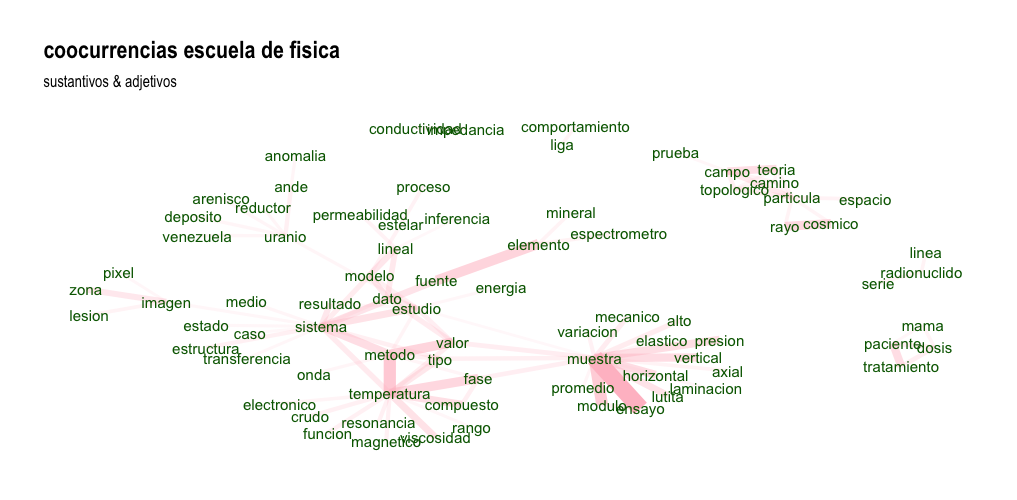
\includegraphics[width=0.9\linewidth]{images/03-marco-teorico/cooc} 

}

\caption{Coocurrencia de Palabras}\label{fig:coocejem}
\end{figure}

\hypertarget{mapacon}{%
\paragraph{Mapas de Conocimiento:}\label{mapacon}}

La representación gráfica y el método de extracción de sustantivos y adjetivos, resulta similar a la propuesta metodológica realizada por \citep{dueñas2011} para crear ``Mapas de Conocimiento'' con ``las palabras claves obtenidas a través de búsquedas recurrentes y relacionadas''. En esta Investigación se simplificará la obtención y representación de estos Mapas, asumiendo que las palabras claves son los sustantivos adjetivizados, equivalente a visualizar las personas, cosas o ideas que se mencionan y que son modificados por los adjetivos, al cambiar sus propiedades o atributos; seleccionando aquellas palabras que muestran una mayor aparición en el \emph{query} realizado y que se interconectan mediante arcos.

\hypertarget{similitud}{%
\subsection{Similitud de documentos:}\label{similitud}}

Para poder realizar la recomendación de documentos, una de las técnicas que se usa es medir la similitud que presenta un documento con los otros contenidos en el corpus \citep{aggarwal2018a} . Un ejemplo de esta técnica es el uso de la similitud coseno que se explica con esta fórmula.

\begin{equation}
\cos ({\bf t},{\bf e})= {{\bf t} {\bf e} \over \|{\bf t}\| \|{\bf e}\|} = \frac{ \sum_{i=1}^{n}{{\bf t}_i{\bf e}_i} }{ \sqrt{\sum_{i=1}^{n}{({\bf t}_i)^2}} \sqrt{\sum_{i=1}^{n}{({\bf e}_i)^2}} }
\end{equation}

En la fórmula \emph{t} representa un documento y \emph{e} representa otro documento. Ambos documentos se asumen que están en un espacio con \emph{i} atributos, o dimensiones, y la intención es calcular un índice de similitud entre ambos documentos.

Este es uno de los métodos más usados para detectar similitudes en los textos, aunque existen otras fórmulas para el cálculo de la similitud como los es el índice de Jaccard.

Al hacer la comparación de un documento i del Corpus que contiene n documentos, en un proceso iterativo con otra cantidad de (\emph{n-1)} documentos, se obtendrán (\emph{n-}1) índices de similitud. Aquel que obtenga un mayor valor se puede inferir que presenta una mayor similitud con el documento \emph{i.}

El otro elemento de gran importancia en el resultado que se obtenga de esta medición, es la representación computacional que se haga del documento. Son distintas las técnicas que existen estando entre ellas la representación mediante ``bolsas de palabras'' o \emph{bag of words,} similar a lo que se explicó en \ref{tdm} donde un documento i es el vector correspondiente a una fila de la matriz y la cantidad de dimensiones que presenta es equivalente al tamaño del vocabulario.

La aplicación de realizar este tipo de comparaciones mediante la estimación de la similitud, es que ante un proceso de \emph{query} también pueden ser recuperados, o sugerir al investigador, en la entrega de los documentos recuperados, aquellos documentos que también presenten alguna similitud, a manera de que el propio sistema tenga la capacidad de realizar recomendaciones.

Recientemente se han creado formas más complejas para la representación de los documentos, como lo son los \emph{word embeddings} que son obtenidos mediante el entrenamiento de redes neuronales de aprendizaje profundo, lo que será expuesto en \ref{embed}.

\hypertarget{SD}{%
\section{Sistemas Distribuidos:}\label{SD}}

Los distintos procesos y componentes de la Solución propuesta han sido diseñados e implementados como un sistema distribuido y por eso se hace la mención a este tema.

Una definición formal que se le puede dar a los sistemas distribuidos es ``cuando los componentes de hardware y/o sofware se encuentran localizados en una red de computadores y estos coordinan sus acciones sólo mediante el pase de mensajes'' \citep{distribu2012}.

Algunas de las principales características que tienen los sistemas distribuidos es la tolerancia a fallos, compartir recursos, concurrencia, ser escalables \citep{czaja2018} entre otras. Mencionamos estas, en particular, al ser propiedades que están presentes en la propuesta acá descrita:

\begin{enumerate}
\def\labelenumi{\arabic{enumi}.}
\item
  Fiabilidad o la llamada tolerancia a fallos: en caso de fallar un componente del sistema los otros se deben mantener en funcionamiento.
\item
  Compartir recursos: un conjunto de usuarios pueden compartir recursos como archivos o base de datos.
\item
  Concurrencia: poder ejecutar varios trabajos en simultáneo.
\item
  Escalable: al ser incrementada la escala del sistema se debe mantener en funcionamiento el sistema sin mayores contratiempos.
\end{enumerate}

\hypertarget{contenedores}{%
\subsection{Contenedores:}\label{contenedores}}

Un contenedor es una abstracción de una aplicación que se crea en un ambiente virtual, en el cual se encuentran ``empaquetados'' todos los componentes (sistema operativo, librerías, dependencias, etc.), que una aplicación necesita para poder ejecutarse. En su diseño se tiene presente que sean ligeros y que con otros contenedores pueden compartir el \emph{kernel}, usando un sistema de múltiples capas, que también pueden ser compartidas entre diversos contenedores, ahorrando espacio en disco del \emph{host} donde se alojan los contenedores \citep{nüst2020}.

El uso de los contenedores permite crear, distribuir y colocar en producción aplicaciones de software de una forma sencilla, segura y reproducible. También a cada contenedor se le puede realizar una asignación de recursos (memoria, cpu, almacenamiento) que garantice un óptimo funcionamiento de la aplicación que contienen.

Es importante señalar que el uso de esta tecnología añade un entorno de seguridad al estar cada contenedor en una ambiente isolado.

Para cada contenedor es necesario usar una imagen donde previamente se definen las dependencias (sistema operativo, librerías, lenguajes) necesarias para su funcionamiento.

\hypertarget{orquestador}{%
\subsection{Orquestador:}\label{orquestador}}

Al tener diversos contenedores, donde cada uno aloja una aplicación distinta, puede resultar necesario que todos se integren en un sistema. Para que esta integración sea viable es necesario contar con un orquestador \citep{cook2017}. Su uso permitirá lograr altos grados de portabilidad y reproducibilidad, pudiendo colocarlos en la nube o en centros de datos, garantizando que se pueda hacer el \emph{deploy} de forma sencilla y fiel a lo que se implementó en el ambiente de desarrollo.

En el caso de la Solución propuesta se adoptará el uso de \emph{Docker Compose} como orquestador y en el Capítulo que contiene los Ciclos de Desarrollo \ref{desarrollociclos4} serán expuestas las funcionalidades de cada contenedor y se apreciará la integración que proporciona contar con un orquestador.

\hypertarget{sota}{%
\section{Estado del Arte:}\label{sota}}

Si bien anteriormente las búsquedas de información dentro de un corpus se procesaban determinando la aparición de palabras dentro de un texto, este método ha ido evolucionando para llegar hoy en día a un elevado nivel de abstracción, donde a partir de la necesidad de obtener una información, es decir, de aquello que necesitamos buscar, que antes consistía en hacer \emph{match} con un objeto de información, se ha pasado de los motores de búsqueda (\emph{search engines} ) a los motores de respuestas ( \emph{answering engines} ) \citep{balog2018}, donde el sistema ante una determinada consulta del usuario, va a retornar una serie de resultados enriquecidos, mostrando la identificación de entidades, hechos y cualquier otro dato estructurado que esté de forma explícita, e incluso implícita, mencionado dentro de los textos que conforman el corpus.

Para hablar sobre el Estado del Arte tanto en los Sistemas de Recuperación de Información \ref{infret} así como en el Procesamiento del Lenguaje Natural \ref{nlproc} y en la medición de similitud entre documentos \ref{similitud} es necesario referir la representación de los textos mediante \emph{embeddings}.

\hypertarget{embed}{%
\subsection{Embeddings}\label{embed}}

Para comprender qué son los \emph{embeddings} se debe partir de estudiar la Hipótesis~ Distribucional, la cual se enmarca en al área de la lingüística y enuncia que la similaridad en significados, resulta en que también se presente una similaridad en la distribución lingüística. Dos palabras que sean próximas en significado, entendido como que sean intercambiables en un texto, es un fenómeno que también se detectará en la distribución que presentan dichas palabras dentro de un corpus. Más adelante se mostrará un ejemplo de esto.

De esta Hipótesis surge la propuesta de crear la ``Distribución Semántica'', donde se representa el significado de una palabra, mediante el proceso en que se toma como entrada grandes cantidades de texto y se construye un modelo de distribución, también llamado ``espacio semántico'', que logra extraer la representación semántica del vocabulario en un espacio \emph{n}-dimensional, haciendo que una palabra se muestre como un vector en dicho espacio.

``Semántica'' se entiende como el significado específico que puede tener una palabra en una oración. Al evaluar las siguientes dos frases:

1. ``El modelo de banco de tres asientos está en oferta''

2. ``Voy a depositar dinero al banco''

el significado de la palabra ``banco'' en los ejemplos tiene dos acepciones. Claramente el lingüista Firth J.R. enfrentó este problema en su famosa frase: ``entenderás una palabra por aquellas que la acompañan'', donde hace entrever que para comprender el significado de una palabra hay que revisar el contexto en el que ocurre.

Al recordar \ref{tdm} el modelo Term Document Frecuency (TDF), para representar en un documento la aparición de una determinada palabra, se colocaba en la matríz el valor ``1'' en la posición \emph{i,j} , o se colocaba un ``0'' en su ausencia, correspondiendo la \emph{i} al índice del documento y la \emph{j} al índice de la palabra dentro del vocabulario; no obstante, en este método de representación no se puede lograr inferir la semántica de la palabra, sino simplemente la aparición, o no, dentro del texto, independientemente de la acepción que tenga la palabra ``banco'', que siempre se representaría con un valor ``1'', tanto en un documento que contenga ``El modelo de banco de tres asientos está en oferta'', como en el otro ``Voy a depositar dinero al banco''.

\hfill\break
Lo anterior constituye un problema clave para los procesos de Recuperación de Información ya que si estuviésemos usando el modelo \ref{invind} de Índices Invertidos, que comparte algunos fundamentos del modelo \ref{tdm} \emph{Term Document Frecuency (TDF)}, retomando el ejemplo en que usamos la palabra ``banco'', al intentar encontrar aquellos documentos que mencionen a los ``bancos'' en su acepción de ``Asiento, con respaldo o sin él\ldots{}'', también se recuperaría el documento que habla de la ``empresa que se dedica a realizar transacciones financieras''.

Este ejemplo, bastante trivial, plantea la necesidad de contar con modelos de representaciones con una estructura más compleja y que puedan facilitar mediante los métodos de \emph{Information Retrieval}, la recuperación de los documentos que tengan la mayor relevancia \ref{relevancia} ante un \emph{query} y que también se correspondan con lo que ciertamente se está buscando, como pudiera ser ``fabrica de bancos para parques'' y mejor aún sería si ante una búsqueda con el texto ``fabrica de sillas'', también se recuperará el documento que indica ``El modelo de banco de tres asientos está en oferta'', ya que asiento y silla pueden ocurrir en contextos semánticos similares.

Son los ``\textbf{\emph{embeddings}}'' la representación que hoy constituye el Estado del Arte en el los procesos de Recuperación de Información ya que hacen posible aplicar distintos métodos algebraicos y computacionales para inspeccionar el vocabulario de un determinado corpus y tener nociones más precisas sobre la cercanía de una palabra con otra y hacer mediciones \ref{similitud} de similitud entre un documento, que se ha transformado en partes o en su totalidad en un \emph{embedding}, con otro que tenga el mismo tipo de representación vectorial.~

En el siguiente ejemplo \ref{tab:tblembedding} que se obtiene del trabajo \emph{Distributional Semantics and Linguistic Theory} \citep{boleda2020}, se muestra una versión simplificada de un espacio semántico de dos dimensiones donde están los vectores que se corresponden con tres palabras que son ``\emph{postdoc'', ''estudent''} y''\emph{wealth''}:

\begin{table}

\caption{\label{tab:tblembedding}Embedding bidimensional para representar palabras}
\centering
\begin{tabular}[t]{lrr}
\toprule
Palabra & Dimensión.1 & Dimensión.2\\
\midrule
postdoc & 0.71038 & 1.76058\\
estudent & 0.43679 & 1.93841\\
wealth & 1.77337 & 0.00012\\
\bottomrule
\end{tabular}
\end{table}

Al tener cada palabra un vector de dos componentes, se puede hacer una representación gráfica en un plano, ver figura \ref{fig:embeddingimg}, donde al aplicar la medición de similitud coseno, revisada en \ref{similitud}, se determina que las palabras \emph{postdoc} y \emph{student} se encuentran más próximas y tienen una mayor similitud, que por ejemplo, \emph{postdoc} y \emph{wealth}.

\begin{figure}

{\centering 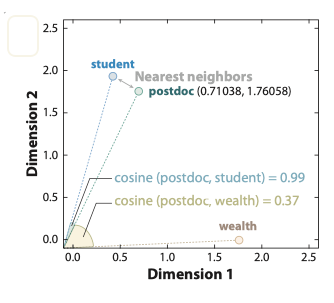
\includegraphics[width=0.55\linewidth]{images/03-marco-teorico/word_vec} 

}

\caption{Representación de palabras en un plano}\label{fig:embeddingimg}
\end{figure}

Al generar la representación completa de un espacio semántico, haciendo la búsqueda de una palabra, podemos encontrar también aquellas que son cercanas y no limitar la búsqueda al \emph{match} que los modelos anteriormente estudiados sí imponían. Más adelante también veremos que el modelo semántico puede ser expandido y representar mediante un \emph{embedding} oraciones (\emph{sentences}), siendo esto el sustento de que al hacer una pregunta, o \emph{query}, a un sistema de Recuperación de Información, este sea capaz de encontrar la respuesta dentro del corpus, ya que la pregunta o \emph{query} se transforma en un \emph{embedding} y luego se determina en el espacio semántico cuál es la oración que más se aproxima, o guarda algún tipo de proximidad o relación de distancia vectorial con la pregunta formulada.~

Los \emph{embeddings} son representaciones numéricas densas de las palabras contenidas en un vocabulario. A diferencia de los modelos de tipo ``one hot encodding (OHE)'' de representación binaria, donde en un vector se usa un ``1'' para representar la aparición de una palabra dentro de un vocabulario y ``0'' para representar su ausencia, teniendo que la dimensionalidad del vector será la cantidad de \emph{n} palabras que tenga el vocabulario. Es común que un corpus se puedan disponer de unas 20 mil o más palabras distintas, es decir un vocabulario con \emph{n} igual a 20 mil, así sea para representar una sola palabra se requerirá en el OHE de unos 20 mil componentes con 19.999 ceros y un solo ``1'', lo cual es una representación bastante dispersa que dificulta cálculos computacionales. Retornando al \emph{embedding}, lo que ellos captan es una representación vectorial de las palabras pero con un número menor de componentes.

En algunas de la primeras representaciones realizadas, por ejemplo con el modelo ``GloVe: Global Vectors for Word Representation'' \citep{pennington2014}, se tenían 100 componentes, cifra considerablemente menor a las 20 mil que del modelo de ``one hot encodding'', evitando así la alta esparcidad. Otro cambio sustancial que se introdujo con este tipo de representación es que los los componentes no son valores binarios de unos o ceros, sino se hace con números reales que pueden tener más de ocho decimales (floating point numbers). Bajo este modelo, la representación específica de la palabra ``king'' es el siguiente vector:

``0.50451, 0.68607, -0.59517, -0.022801, 0.60046, -0.13498, -0.08813, 0.47377, -0.61798, -0.31012, -0.076666, 1.493, -0.034189, -0.98173, 0.68229, 0.81722, -0.51874, -0.31503, -0.55809, 0.66421, 0.1961, -0.13495, -0.11476, -0.30344, 0.41177, -2.223, -1.0756, -1.0783, -0.34354, 0.33505, 1.9927, -0.04234, -0.64319, 0.71125, 0.49159, 0.16754, 0.34344, -0.25663, -0.8523, 0.1661, 0.40102, 1.1685, -1.0137, -0.21585, -0.15155, 0.78321, -0.91241, -1.6106, -0.64426, -0.51042''

el cual se puede representar graficamente como se observa el la figura \ref{fig:embking} donde se mapean los números a una paleta de colores.

\begin{figure}

{\centering 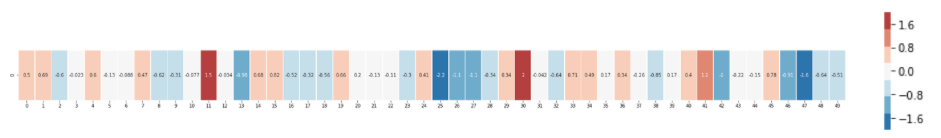
\includegraphics[width=0.95\linewidth]{images/03-marco-teorico/embking} 

}

\caption{Representación de palabra "king" mediante el modelo GloVe}\label{fig:embking}
\end{figure}

Usando el mismo modelo GloVe, una representación gráfica de las palabras ``King'', ``Man'' y ``Woman'' en 50 dimensiones es la que se observa en la imagen \ref{fig:GloVeEmbedd}.

\begin{figure}

{\centering 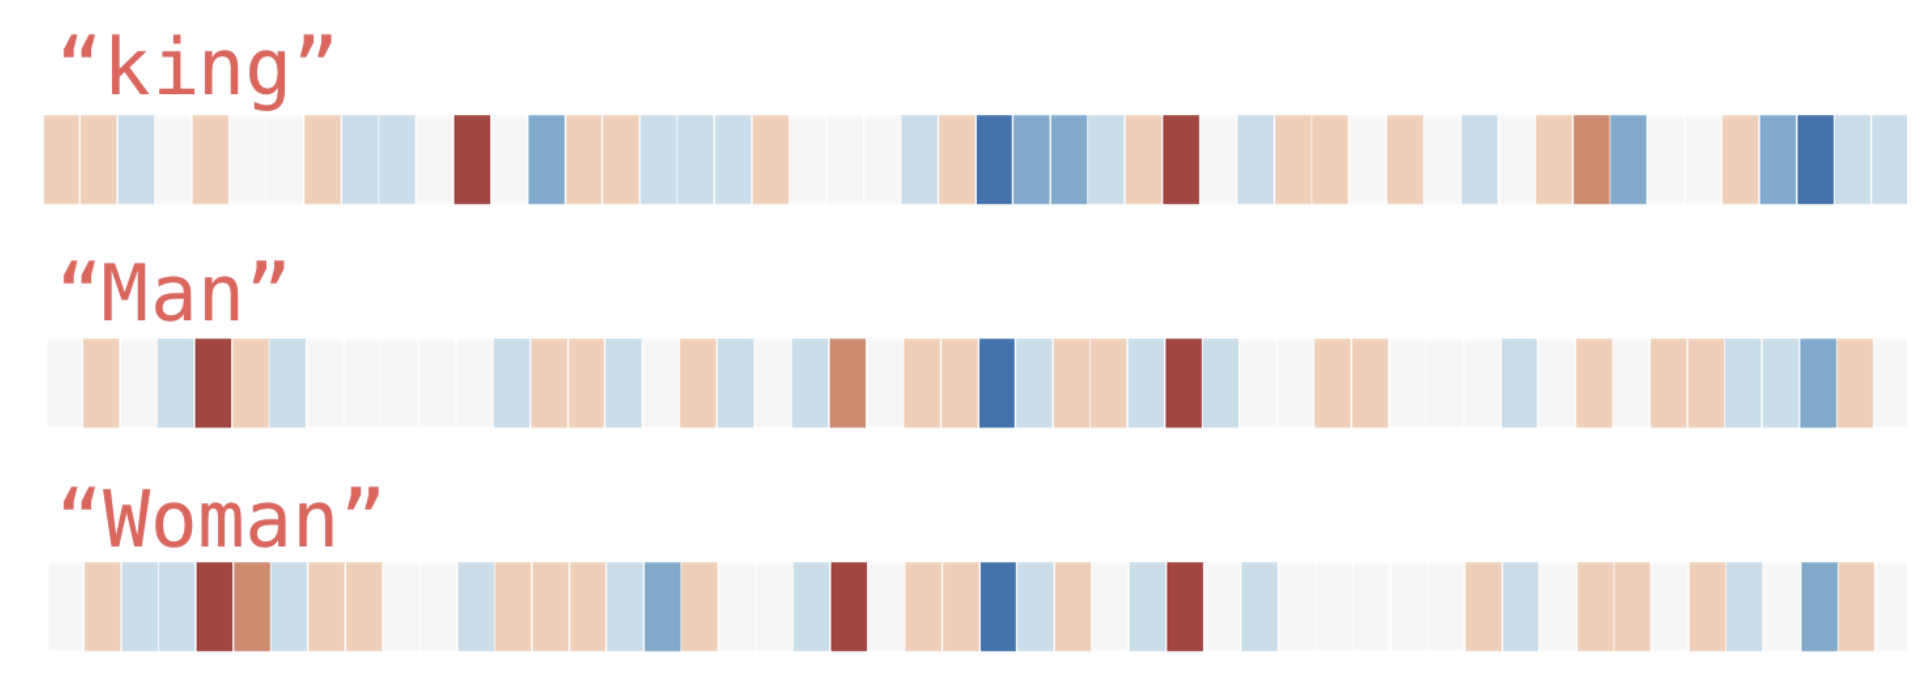
\includegraphics[width=0.95\linewidth]{images/03-marco-teorico/embedding} 

}

\caption{Representación de palabras mediante el modelo GloVe}\label{fig:GloVeEmbedd}
\end{figure}

El crédito a la visualización \ref{fig:GloVeEmbedd} \citep{wordtovec} corresponde al divulgador Jay Alammar. (2019). ~La representación muestra gráficamente que las palabras ``man'' y ``woman'' son más ``parecidas'' visualmente que ``king'' y ``man'' y esto es lo que se puede generalizar para entender como las distintas palabras que se representan en un espacio semántico pueden presentar proximidades, similitudes o diferencias entre si, obteniendo de esta forma un significado semántico según la posición relativa que cada una tenga con respecto a la otra en el espacio indicado.

No obstante, en los puntos expuestos aún no ha explicado cómo se generan los \emph{embeddings}, lo cual es indispensable para entender sus capacidades. En el año 2003 mediante el entrenamiento de redes neuronales logran modelar la probabilidad de las secuencias de palabras demostrando la capacidad de las redes neuronales para capturar patrones complejos en datos textuales \citep{Bengio:2003:NPL:944919.944966} . Otro hito fue la investigación ``Semantic Hashing'' \citep{salakhutdinov2009} donde usaron redes neuronales para transformar datos de alta dimensionalidad en representaciones binarias de baja dimensionalidad. Esa investigación añadió como aporte que se empezarán a usar técnicas de aprendizaje no supervisado para entrenar las redes neuronales, deshaciéndose de los cuellos de botella que previamente introducían los procesos de etiquetado, necesarios en métodos supervisados.

Ante la ampliación de capacidades de computo en sistemas distribuidos compuestos por tarjetas gráficas (Graphics Processing Unit - GPU), empieza a incrementarse el uso de redes neuronales de aprendizaje profundo y es cuando se presenta la investigación ``Word2Vec: Efficient Estimation of Word Representations in Vector Space'' \citep{mikolov2013} que implementa la técnica \emph{Skip-gram} y \emph{Continuous Bag of Words (CBOW)} que permitieron a las redes neuronales el aprendizaje de representaciones semánticas de palabras a partir de grandes volúmenes de texto. Word2Vec no solo era eficiente computacionalmente, sino que también producía \emph{embeddings} que capturaban relaciones semánticas y sintácticas, transformando cómo se abordaban las tareas de NLP y las aplicaciones de recuperación de información.

Una vez que se empezó a tener un método para capturar la semántica de las palabras debió seguir el paso de lograr representar el sentido semántico de frases (sentences) y expresiones más complejas. Esto se introdujo en la investigación ``Distributed Representations of Words and Phrases and their Compositionality'' (2013) \citep{mikolov2013a} donde se hicieron representaciones vectoriales distribuidas para frases, mejorando la capacidad de capturar significados contextuales y relaciones sintácticas en un nivel más alto, lo cual resultó crucial para mejorar los sistemas de recuperación de información y también para la traducción automática.

La investigación GloVe \citep{pennington2014} también implicó grandes avances ya que superó limitaciones que presentaban investigaciones anteriores, al permitir generar analogías del tipo: (vector de embedding para la palabra Rey) menos (vector de embedding para la palabra hombre) más (embedding para la palabra mujer) es igual, o muy aproximado en el espacio semántico, al (vector de embedding de la palabra reina) o simplificado como ``rey-hombre+mujer=reina''.

Igualmente con esta investigación se intensificó el uso de este modelo en tareas de clasificación de texto como las revisadas en \ref{nlproc}, ya que las redes neuronales empezaron a entrenarse con representaciones de vectores de gran densidad que contenían las palabras, el POS y el etiquetado de las dependencias conteniendo cada vector 200 componentes, alcanzando mejores indicadores de desempeño en el etiquetado \citep{chen2014}. Este trabajo fue el que dio soporte a la librería revisada anteriormente de nombre ``coreNLP'' de la Universidad de Stanford.

\hypertarget{trans}{%
\subsection{\texorpdfstring{Arquitectura de Redes Neuronales \emph{Transformers}:}{Arquitectura de Redes Neuronales Transformers:}}\label{trans}}

En el año 2017 se publica ``Attention Is All You Need'' \citep{vaswani2017} el cual fue una investigación donde se introdujo una nueva arquitectura de redes neuronales que eliminó ciertas limitaciones que venían presentando los modelos de redes neuronales recurrentes y las convolucionales en poder trabajar con largas cadenas de texto. La solución introdujo los llamados ``mecanismos de atención'' \footnote{Los mecanismos de atención permiten al modelo asignar ponderaciones dinámicas a diferentes partes de la entrada, lo que resulta en una comprensión más profunda y contextualizada del texto.} que abrieron el camino para la creación de nuevos modelos de lenguaje como BERT \citep{devlin2018} que capturaban la riqueza de significados y las relaciones complejas del lenguaje mejorando la comprensión de textos, traducción automática y la generación de texto.

``RoBERTa: A Robustly Optimized BERT Pretraining Approach'' \citep{liu2019} optimizó el entrenamiento preexistente de BERT al desvincular la tarea de pre-entrenamiento del tamaño de la cantidad de ejemplos de entrenamiento (\emph{batch size}) y la duración del entrenamiento. Al escalar el tamaño del lote y la cantidad de datos, RoBERTa mejoró la comprensión del modelo sobre el lenguaje, logrando una capacidad de generalización excepcional. Estos métodos que venían innovando e incrementando las capacidades, por otra parte también hacían que el tamaño de los conjuntos de datos usados para el entrenamiento fuese creciendo exponencialmente, como se analizará en \ref{LLM} la sección referida a los Largos Modelos del Lenguaje.

Otro modelo basado en la arquitectura de Transformers, que es necesario referir, ya que a un componente del SCSU le da soporte, es el que se publicó bajo el título ``Sentence-BERT: Sentence Embeddings'' \citep{reimers2019a} que a diferencia de los modelos anteriormente expuestos, que trabajaban con la codificación de palabras, en él se logra la codificación de oraciones usando una variante de BERT \citep{devlin2018}. Al entrenar el modelo para entender la similitud semántica entre pares de oraciones, Sentence-BERT aprende representaciones de oraciones que capturan mejor las relaciones semánticas.

Un punto que fue necesario resolver, era lograr contar con representaciones de embeddings para distintos idiomas, ya que inicialmente estaban entrenados con textos en idioma ingles y uno de las investigaciones que permitió avanzar hacia modelos multilingües fue ``Making Monolingual Sentence Embeddings Multilingual'' \citep{reimers2020}, usando la técnica ``Knowledge Distillation'', en lugar de entrenar modelos para cada idioma, este método utiliza un único modelo de referencia monolingüe para guiar el entrenamiento de modelos en múltiples idiomas, basándose en la idea de que ``una frase traducida debe situarse en el mismo lugar del espacio vectorial que la frase original''.

Este recorrido por el desarrollo de los embeddings lleva finalmente al modelo ``BETO: Spanish BERT'' \citep{CaneteCFP2020}, que bajo la arquitectura BERT fue entrenado por el Departamento de Ciencias de la Computación Universidad de Chile, disponible en el enlace \url{https://github.com/dccuchile/beto} . Este modelo para la fecha está considerado como el estado del arte para el idioma español, alcanzando una precisión del 98,97\% en tareas como el POS \ref{pos}.

Las investigaciones citadas se hicieron de dominio público y en muchos casos también se colocó a disposición de la comunidad científica los propios modelos preentrenados, lo que hizo que fuesen reproducibles tantos los modelos, como la evaluación de ellos.

Para obtener información sobre los modelos de \emph{embeddings} que presentan una elevada precision y son de alta demanda por la comunidad open source, siendo parte del estado del arte, se tienen herramientas como el ``MTEB: Massive Text Embedding Benchmark'' \citep{muennighoff2022} al que se puede acceder en el enlace \url{https://huggingface.co/spaces/mteb/leaderboard} donde muestra métricas de 140 modelos preentrenados en el área del lenguaje disponibles para el uso público.

\hypertarget{LLM}{%
\subsection{Largos Modelos de Lenguaje:}\label{LLM}}

Con la aparición de la arquitectura Tranformers se abrió el camino para la aparición de los Largos Modelos de Lenguaje \emph{(Large Language Modes -LLM´s)}. En principio pudiese parecer estar fuera del alcance de este Trabajo de Grado exponer estos Modelos, pero el Estado del Arte de los Sistemas de Recuperación de Información se intersecta con ellos y no resultan ajenos a trabajos futuros que puedan suceder a esta investigación.

Según lo revisado en la sección de \emph{embeddings} \ref{embed}, la tendencia ha sido ir incrementando la cantidad de datos con que se entrenan estos modelos, igual que la cantidad de parámetros que conforman al propio modelo. En la figura \ref{fig:llm} vemos las variaciones increméntales que se han dado desde la publicación del modelo basado en los Transformers en el 2017.

\begin{figure}

{\centering 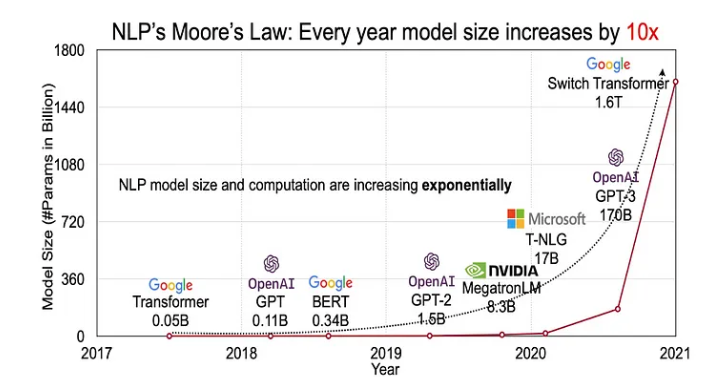
\includegraphics[width=0.85\linewidth]{images/03-marco-teorico/llms} 

}

\caption{Evolución en la Cantidad de parámetros en los LLM}\label{fig:llm}
\end{figure}

El crédito a la visualización \ref{fig:llm} corresponde a Harishdatala (2023). Unveiling the Power of Large Language Models (LLMs). \url{https://medium.com/@harishdatalab/unveiling-the-power-of-large-language-models-llms-e235c4eba8a9} (acceso 23 el octubre, 2023).

Sin entrar en mayores consideraciones sobre este crecimiento y los costos asociados, que imposibilitan a instituciones educativas, empresas de mediano tamaño, investigadores independientes, poder acceder a los sistemas de computadores necesarios para entrenar modelos de estas características, a finales del año 2022 a uno de los modelos llamado ``Generative Pre-trained Transformer 3'' de la empresa OpenAI, del cual no se dispone mayor documentación sobre su arquitectura ni precisión sobre el método de entrenamiento, le es realizado un proceso de ``fine tunning'', que es un ajuste a los parámetros mediante un reentrenamiento, y se creó lo que hoy se conoce comercialmente como ChatGPT 3.5, introduciendo mediante una interface de usuario, la capacidad de que un usuario pueda interactuar con el modelo simulando una conversación. Abstrayendo los procesos de entrenamiento, la magnitud de los parámetros y la innovación que representó crear el modelo de chat, lo que se tiene es un usuario interactuando con un modelo semántico de una magnitud gigante.

En general los Largos Modelos de Lenguaje son entrenados con enormes corpus de textos recopilados de foros de internet, de páginas web, de libros digitalizados y de un basto cúmulo de textos. Si hacemos otra abstracción de un nivel más alto, lo que se tiene es un usuario haciendo un \emph{query} ante un enorme Corpus que excede y se organiza de una forma distinta a lo que habíamos revisado en los Sistemas de Recuperación de Información \ref{SRI} clásicos donde se tenía una base de dato con documentos indexados. Ahora son distintos tanto el proceso de interacción usuario-computador y más importante aún es que también cambia la representación de la información, ya que cada vez que se coloca un \emph{query}, este es transformado en un \emph{embedding}, y mediante un proceso estocástico, el LLM va prediciendo la siguiente palabra, de una en una, y se van construyendo respuestas, que pueden llegar a ser fidedignas, o no tanto, dependiendo de la calidad del modelo y de las previsiones que se hayan tomado para mitigar sesgos o entradas de datos incorrectas en la fase de entrenamiento del modelo.

Como queda fuera del alcance de este trabajo explicar como funcionan los modelos del lenguaje, lo que sí se quiere indicar es que en el año 2023 algunas compañías e institutos de investigación privada, empezaron a liberar ciertos modelos, con distintos pesos y versiones, para la comunidad open source, como lo es el modelo Falcon \citep{penedo2023} o el modelo OpenLlama2 \citep{touvron2023} \footnote{la compañía que entrenó el modelo y lo liberó que es Meta indicó que es OpenSource, pero revisiones técnicas hechas a la licencia cuestionan que se pueda considerar que realmente cumpla las especificaciones para que sea considerado plenamente ``open source''. En el enlace \href{https://opensourceconnections.com/blog/2023/07/19/is-llama-2-open-source-no-and-perhaps-we-need-a-new-definition-of-open/}{Is Llama 2 open source?} se encuentra un análisis sobre el tema.}. Con las facilidades para el desarrollo que aportan plataformas como \url{huggingface.com} para la implementación de aplicaciones de inteligencia artificial, mediante el almacenamiento de modelos preentrenados, conjuntos de datos para entrenamiento o sobre entrenamiento, así como librerías con \emph{pipelines} de fácil integración mediante API´s unificadas \citep{wolf2019}, estos LLM´s dejaron de tener un uso limitado sólo para grandes empresas o consorcios tecnológicos y para la fecha es viable que corran en computadoras con capacidades limitadas mediante métodos como la aplicación del quantized que se presenta en la investigación \citep{dettmers2023} que permite que un LLM que por ejemplo necesite unos 16 gb de memoria ram en GPU para ser desplegado, pueda disminuir una cuarta parte hasta los 4 gb.

La diversidad de modelos preentrenados, con distintas versiones de fine tunning o cuantizaciones, se puede ver en el enlace \citep{openllm} \url{https://huggingface.co/spaces/HuggingFaceH4/open_llm_leaderboard} donde se encuentra un tablero que muestra los modelos que presentan mayor popularidad, descargas y métricas de evaluación de su comportamiento.

\hypertarget{int}{%
\subsection{Integración:}\label{int}}

Las versiones \emph{Open Source} de estos modelos es posible integrarla en procesos de \emph{Information Retrieval} principalmente mediante tres técnicas.

\begin{enumerate}
\def\labelenumi{\arabic{enumi}.}
\item
  \textbf{Retrieval Augmented Generation RAG} \citep{lewis2020}: esta técnica permite que un LLM que fue entrenado con un determinado corpus, pueda activar la extracción de información desde fuentes externas, como páginas de internet, complementando la información que dispone el modelo. A nivel de interacción del usuario todo ocurre en el mismo entorno o API que dispone el modelo originalmente.
\item
  \textbf{Fine Tunning} \citep{lv2023}: con un conjunto de datos etiquetado, de un volumen de datos mucho menor al que inicialmente fue entrenado un determinado LLM, se puede lograr que un modelo de lenguaje aprenda, sea sobreentrenado con métodos como el propuesto en ``Universal Language Model Fine-tuning for Text Classification'' \citep{howard2018}, con información de un dominio específico, mejorando su desempeño en esa particular área.
\item
  \textbf{Vector DataBase:} mediante una representación de datos en \emph{embeddings} se crea una base de datos con los documentos que están contenidos en corpus. El manejador de base de datos ofrece un almacenamiento optimizado y capacidades de consulta para estructuras únicas de \emph{embeddings} vectoriales, permitiendo hacer búsquedas semánticas, alto rendimiento, escalabilidad y recuperación de datos al comparar valores y encontrar similitudes.
\end{enumerate}

Principalmente estas tres técnicas, por separado, o en paralelo, pueden implementarse para crear sistemas de recuperación de información que se adapten y sean expertos en áreas de estudio de la Universidad Central de Venezuela, modificando la forma en que anteriormente un investigador hacía la búsqueda de información.

\hypertarget{busquedasemantica}{%
\subsection{Búsqueda Semántica:}\label{busquedasemantica}}

Es una evolución en la forma en que los motores de búsqueda comprenden y responden a las consultas. A diferencia de la búsqueda tradicional basada en palabras clave, que se centra en encontrar coincidencias literales entre la consulta y el contenido web, la búsqueda semántica tiene como objetivo comprender el significado contextual de las consultas y ofrecer resultados más relevantes y precisos.

En lugar de simplemente emparejar palabras clave, la búsqueda semántica utiliza \emph{embeddings} para representar el texto y de una mejor forma comprender la intención detrás de una consulta. Esto implica analizar la relación semántica entre las palabras, interpretar el contexto y comprender el significado subyacente. Así, la búsqueda semántica busca proporcionar resultados que no solo coincidan con las palabras clave, sino que también aborden la verdadera intención del usuario.

Se apoya en representar cadenas de texto de un documento como vectores \emph{embeddings} que son almacenados en una base de dato y dado un \emph{query} se transforma el texto en otro \emph{embedding} y se determina cuáles son los embeddings de la base de dato que presentan mayor similitud \citep{muennighoff2022a}.

Finalmente se mencionan algunos puntos de lo que hoy constituye el estado del arte en temas que hemos ido revisando a lo largo de este capítulo:

\begin{enumerate}
\def\labelenumi{\arabic{enumi}.}
\item
  Con modelos como BERT se ha hecho implementaciones modificadas para hacer el re ordenamiento \ref{ranking} de los resultados obtenidos en un proceso de búsqueda, bien sea mediante las técnicas tradicionales o mediante técnicas de búsqueda semántica\citep{nogueira2019} . Igualmente con redes neuronales se ha buscado simular el comportamiento humano para jerarquizar los resultados obtenidos en procesos de búsqueda \citep{pang2017}.
\item
  Se están proponiendo nuevos métodos para evaluar la eficacia en los sistemas de ``preguntas-respuestas'' basados en similaridad semántica dadas las limitaciones que presentan las métricas tradicionales que no reflejan el desempeño de estos nuevos modelos \citep{risch2021}.
\item
  Mediante técnicas de aprendizaje profundo se están creando conjuntos de datos sintéticos de dominio público que permitan evaluar el desempeño de los sistemas de recuperación de información, usando como entrada las publicaciones de Wikipedia y creando con estos modelos los \emph{querys}, que permitan medir el grado de precisión que alcanza un determinado sistema \citep{frej-etal-2020-wikir}.
\end{enumerate}

Así culmina el recorrido por lo que es el Marco Teórico-Referencial \ref{teorico} que soporta la investigación ``Recuperación, Extracción y Clasificación de Información de SABER UCV''.

\hypertarget{mm}{%
\chapter{Capítulo Marco Metodológico:}\label{mm}}

En este capítulo, se presenta el enfoque metodológico adoptado para este estudio. La metodología Kanban \ref{mmmetodologia} se empleó para gestionar el proceso general, mientras que la metodología de Desarrollo Adaptable de Software \ref{mmasd} guió la creación del software, permitiendo una implementación eficiente y adaptable a las necesidades cambiantes del proyecto \textbf{Recuperación, Extracción y Clasificación de Información de SABER UCV}.

\hypertarget{mmmetodologia}{%
\section{Metodología de Trabajo Kanban:}\label{mmmetodologia}}

En esta metodología se fomenta la cultura de mejora continua, incremental, al identificar cuellos de botella y la limitación del trabajo en curso para aumentar la eficiencia y la productividad. Gracias a su enfoque basado en la colaboración, flexibilidad y respuesta rápida a los cambios, puede considerarse que está dentro de las metodologías ``Ágiles''.

Mediante la visualización del flujo de trabajo en un tablero, que se aprecia en la figura \ref{fig:metkanban}, se puede facilitar la gestión del proyecto, desde la concepción de una idea, hasta su implementación y entrega. En el caso del desarrollo de software, facilita la toma de decisiones informadas y promueve la transparencia al proporcionar una visualización clara de las tareas y actividades involucradas \citep{stephens2015}.

\begin{figure}

{\centering 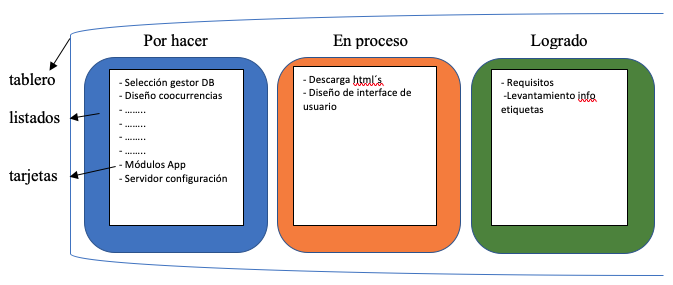
\includegraphics[width=0.7\linewidth]{images/04-metodologia/01_kanban} 

}

\caption{Representación de un tablero según la metodología Kanban}\label{fig:metkanban}
\end{figure}

Durante el desarrollo de este Sistema se necesitaba contar con la flexibilidad que ofrece esta metodología, ya que en ella no se tienen que definir roles específicos en el equipo desarrollador, ni tampoco es necesario establecer períodos fijos para alguna fase en particular.

\hypertarget{mmasd}{%
\section{Desarrollo Adaptable de Software:}\label{mmasd}}

El \textbf{Adaptive Software Development (ASD)} \citep{highsmith2000} es una metodología ágil de desarrollo de software que se centra en la adaptabilidad y capacidad para adaptarse a los cambios, proporcionando una retroalimentación temprana y frecuente, dando flexibilidad para abordar los desafíos cambiantes del desarrollo de software. A diferencia de los enfoques tradicionales, el ASD reconoce la naturaleza impredecible del desarrollo de software y se adapta continuamente para satisfacer las necesidades del cliente en un entorno dinámico y complejo, haciendo énfasis en el principio ``Entregar el proyecto que se necesita al final, no el proyecto que se pidió al principio''.

\hypertarget{caracteruxedsticas}{%
\subsection{Características:}\label{caracteruxedsticas}}

\textbf{Colaboración y Comunicación Constante:} fomenta la colaboración cercana entre los equipos de desarrollo y los \emph{stakeholders}. La comunicación constante permite una comprensión profunda de los requisitos del cliente y facilita ajustes rápidos según las necesidades cambiantes.

\textbf{Iteraciones Incrementales:} divide el proyecto en iteraciones cortas y manejables. Cada iteración produce un incremento funcional del software, lo que permite obtener retroalimentación temprana que permite corregir errores y ajustar el rumbo del proyecto antes de que los problemas se vuelvan críticos.

\textbf{Flexibilidad y Adaptabilidad:} reconoce que los requisitos del proyecto pueden cambiar con el tiempo. Por lo tanto, se adapta fácilmente a los cambios, permitiendo una rápida reevaluación y ajuste de las estrategias y metas del proyecto asegurando que el producto final esté alineado de manera óptima con las necesidades y expectativas del cliente, incluso en un entorno de desarrollo volátil.

\hypertarget{ciclos}{%
\subsection{Ciclos:}\label{ciclos}}

El desarrollo adaptable de software se basa en un proceso dinámico e iterativo donde cada ciclo contiene las siguientes fases: Especular-Colaborar-Aprender. El proceso se enfoca en el aprendizaje continuo y la colaboración intensiva entre desarrolladores y clientes, fundamental para enfrentar las cambiantes dinámicas empresariales. Es relevante destacar que, en algunas circunstancias, los ciclos pueden avanzar simultáneamente en ciertas iteraciones, permitiendo así una optimización del tiempo y recursos.

En cada ciclo, se pueden realizar múltiples iteraciones con el objetivo de desarrollar exhaustivamente todos los requisitos contemplados.

Estos ciclos representan un enfoque metodológico que asegura la coherencia y calidad del desarrollo del sistema. A través de la especulación, la colaboración y el aprendizaje continuo, se logra un refinamiento progresivo de las funcionalidades del sistema, garantizando así su robustez y adaptabilidad a las demandas del entorno. Este enfoque iterativo y colaborativo constituye una práctica fundamental en el proceso de desarrollo, facilitando la identificación temprana de posibles desafíos y fomentando la innovación constante en cada etapa del ciclo.

\begin{figure}

{\centering 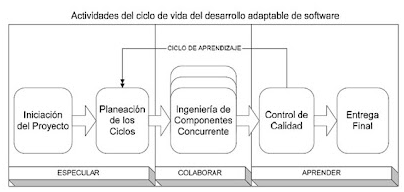
\includegraphics[width=0.6\linewidth]{images/04-metodologia/02_ciclo} 

}

\caption{Ciclo ASD}\label{fig:metdas}
\end{figure}

\hypertarget{especulaciuxf3n}{%
\subsubsection{\texorpdfstring{\textbf{Especulación:}}{Especulación:}}\label{especulaciuxf3n}}

Este componente ofrece un espacio para la exploración y la comprensión de la incertidumbre. Permite desviarse del plan inicial sin temor, transformando los errores en oportunidades de aprendizaje. Aceptar que no se sabe todo impulsa la disposición para aprender y experimentar.

\hypertarget{colaboraciuxf3n}{%
\subsubsection{\texorpdfstring{\textbf{Colaboración:}}{Colaboración:}}\label{colaboraciuxf3n}}

Las aplicaciones complejas requieren la recopilación y el análisis de grandes volúmenes de información y ejecución de tareas. Este proceso es inmanejable para un individuo. En entornos dinámicos, donde fluyen grandes cantidades de datos, es esencial la colaboración. Un solo individuo o un pequeño grupo no puede abarcar todo el conocimiento necesario.

\hypertarget{aprendizaje}{%
\subsubsection{\texorpdfstring{\textbf{Aprendizaje:}}{Aprendizaje:}}\label{aprendizaje}}

La evaluación continua del conocimiento a través de retroalimentaciones y reuniones grupales al final de cada ciclo iterativo es esencial. Este enfoque difiere de la evaluación al final del proyecto. Evaluar constantemente permite enfrentar y resolver de manera efectiva los cambios constantes del proyecto y su adaptación.

\hypertarget{desarrollo}{%
\chapter{Desarrollo de la Solución:}\label{desarrollo}}

En este Capítulo en \ref{desarollodescripcion} se presenta la \textbf{Descripción General de la Solución}. Posteriormente se muestra la \ref{desarrolloarquitectura} \textbf{Arquitectura de la Solución} con el ``Modelo-Vista-Controlador''. En \ref{desarrollociclos} se exponen los cuatro \textbf{Ciclos de Desarrollo} que se efectuaron, mientras que en \ref{pruebas} \textbf{Pruebas} se encuentran las distintas pruebas que fueron ejecutadas para medir el comportamiento y redindimiento del software desarrollado.

\hypertarget{desarollodescripcion}{%
\section{Descripción General de la Solución:}\label{desarollodescripcion}}

Se implementa un Sistema de Recuperación de Información sobre un corpus de documentos de tesis de grado y trabajos de grado que originalmente se encuentran alojados en el repositorio digital Saber UCV . Utilizando técnicas de extracción de datos de archivos HTML, desde la ficha de cada investigación, se obtiene: el título, el nombre del autor, palabras clave, fecha de publicación, el resumen y el url de descarga del documento que sustenta la investigación.

Posteriormente el Sistema descarga el documento referenciado en cada ficha, el cual contiene el texto completo de la investigación, da lectura y clasifica información sobre el nombre de la facultad, la escuela o postgrado donde fue realizado el trabajo e igualmente extrae el nombre del tutor.

Todos los datos obtenidos son sometidos a técnicas del estado del arte en el Procesamiento del Lenguaje Natural y la Minería de Texto para conformar un corpus anotado, un índice invertido y una tabla con los vectores de \emph{embeddings} (vector database), esenciales para un eficiente manejo de la base de datos.

El Sistema incluye una aplicación web que permite a los usuarios desde un navegador explorar extensivamente el corpus anotado, realizando consultas de texto y aplicando varios filtros como la selección de la jerarquía, el área académica y el rango de fechas.

La relevancia de los resultados recuperados se determina mediante una función de ponderación y los documentos se presentan de manera priorizada para mejorar la experiencia del usuario.

Adicionalmente, el Sistema ofrece recomendaciones de documentos que presentan similitud con aquellos que fueron recuperados en el proceso anterior y muestra ``Mapas de Conocimiento'' mediante una herramienta gráfica interactiva de visualización.

La solución implementada cuenta con procesos automatizados de actualización para incorporar las nuevas investigaciones que sean añadidas al repositorio Saber UCV.

El Sistema se soporta en un sistema distribuido conformado por contenedores que son gestionados por un orquestador con la arquitectura ``modelo-vista-controlador''.

\hypertarget{desarrolloarquitectura}{%
\section{Arquitectura de la Solución:}\label{desarrolloarquitectura}}

La arquitectura ``Modelo-Vista-Controlador'' se muestra en la figura \ref{fig:arquitecturamvc} y posteriormente se describe el comportamiento y las interacciones de los componentes.

\begin{figure}

{\centering 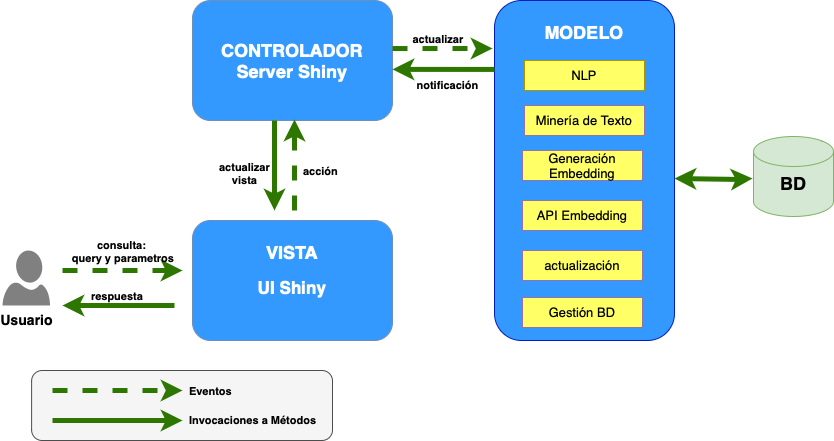
\includegraphics[width=0.9\linewidth]{images/05-desarrollo/MVC9} 

}

\caption{Modelo de Arquitectura MVC}\label{fig:arquitecturamvc}
\end{figure}

\hypertarget{modelo}{%
\subsection{\texorpdfstring{\textbf{Modelo:}}{Modelo:}}\label{modelo}}

El \emph{Modelo,} en el contexto de esta propuesta, es la parte del Sistema que se ocupa de la obtención, manipulación y gestión de los datos. Esto incluye la descarga de la información, la clasificación, el Procesamiento del Lenguaje Natural, la Minería de Texto y la creación del índice invertido. Esta parte del Sistema también incluye la lógica para generar los \emph{embeddings} y manejar el corpus anotado. En la implementación el manejador de base de datos que usa es PostgreSQL.

Igualmente le corresponde realizar las tareas de actualizar el corpus periódicamente y las recomendaciones de documentos a medida que se agreguen nuevos textos en Saber UCV. En \ref{desarrollociclos4} el tercer ciclo de desarrollo se expondrán con detalle los componentes del \emph{Modelo} y a continuación se enumeran los principales procesos que él sustenta:

\begin{enumerate}
\def\labelenumi{\arabic{enumi}.}
\item
  \textbf{Creación del Índice Invertido:}

  \begin{itemize}
  \item
    Organizar los términos y sus ubicaciones en los documentos para permitir búsquedas eficientes.
  \item
    Asociar cada término con la lista de documentos en los que aparece.
  \end{itemize}
\item
  \textbf{Procesamiento de Texto:}

  \begin{itemize}
  \item
    Tokenización: Dividir el texto en palabras o frases significativas.
  \item
    Lematización: Reducir las palabras a su forma base para un análisis más preciso.
  \item
    POS: etiquetado de partes del discurso.
  \end{itemize}
\item
  \textbf{Minería de Texto:}

  \begin{itemize}
  \tightlist
  \item
    Análisis de Frecuencia: Determinar la frecuencia de ocurrencia de palabras o frases.
  \end{itemize}
\item
  \textbf{Generación de Embeddings:}

  \begin{itemize}
  \item
    Utilización de un modelo preentrenado para convertir palabras o frases en vectores numéricos.
  \item
    Convertir en vectores las palabras que componen el \emph{query} para realizar comparaciones semánticas y determinar similitudes entre palabras o documentos.
  \end{itemize}
\item
  \textbf{Gestión de la Base de Datos:}

  \begin{itemize}
  \item
    Almacenar y recuperar datos estructurados para su posterior consulta.
  \item
    Actualizar el corpus con nuevos datos.
  \end{itemize}
\item
  \textbf{Cálculo de Relevancia:}

  \begin{itemize}
  \item
    Aplicar algoritmos para calcular la relevancia de los documentos en función de las consultas del usuario.
  \item
    Ordenar los resultados en función de su relevancia para presentar los documentos más relevantes primero.
  \end{itemize}
\item
  \textbf{Actualización de datos:}

  \begin{itemize}
  \item
    Los procesos mencionados previamente son ejecutados y/o actualizados periódicamente.
  \item
    Se realiza la validación de la integridad de datos para asegurar que los nuevos datos se integren correctamente sin errores o inconsistencias, eliminando posibles duplicados o valores incorrectos.
  \end{itemize}
\end{enumerate}

\hypertarget{vista}{%
\subsection{\texorpdfstring{\textbf{Vista:}}{Vista:}}\label{vista}}

La \emph{Vista} se implementa mediante el \emph{framework} ``Shiny'' \citep{shiny} \footnote{El framework Shiny incluye dos componentes principales. El primero es la UI (interfaz de Usuario), que corresponde a la ``Vista''. El otro componente es el ``Server'' que en la representación actual es el Controlador.} que permite crear aplicaciones web interactivas y tiene un componente de ``User Inferface (UI)'' donde el usuario interactúa al introducir el texto con el que se hará la búsqueda y aplica filtros como jerarquía, área académica y rango de fechas. Posterior a la definición de los atributos del \emph{query}, se desencadenan acciones que son enviadas al \emph{Controlador} y al recibir la respuesta la \emph{Vista} se actualiza y muestra las tablas con los resultados de las búsqueda, las representaciones visuales como el ``Mapa del Conocimiento'' y las recomendaciones de documentos similares.

\hypertarget{controlador}{%
\subsection{\texorpdfstring{\textbf{Controlador:}}{Controlador:}}\label{controlador}}

El \emph{Controlador} se implementa mediante el el \emph{framework} ``Shiny'' que tiene un componente denominado ``Server'' que es el responsable de manejar las interacciones del usuario, gestionar las consultas de texto y aplicar los filtros seleccionados. También se encarga de orquestar las operaciones entre el \emph{Modelo} y la \emph{Vista}, asegurando que los datos se presenten correctamente y que las consultas se procesen de manera eficiente. Desde el \emph{Controlador} se hace el llamado al componente del \emph{Modelo} donde se encuentra la API para generar el \emph{embedding} del \emph{query} y determinar la relevancia de los documentos recuperados. El \emph{Controlador} aplica el re ordenamiento para mostrar en orden los resultados más relevantes. En él se conforma la estructura para representar el ``Mapa del Conocimiento'' con datos obtenidos del \emph{Modelo}.

\hypertarget{desarrollociclos}{%
\section{Ciclos de Desarrollo:}\label{desarrollociclos}}

Los Ciclos de Desarrollo \ref{mm} constituyen fases críticas del proceso, donde se conciben, diseñan y perfeccionan las funcionalidades del Sistema. Cada uno de estos ciclos está estructurado en tres etapas fundamentales: la etapa de especulación, donde se plantean las ideas y se exploran posibles soluciones; la etapa de colaboración, donde se trabaja en equipo para implementar estas ideas y se evalúan los resultados; y la etapa de aprendizaje, donde se analizan las experiencias pasadas y se ajustan las estrategias para futuras iteraciones.

Para el desarrollo del SCSU se hizo un proceso iterativo donde en cada ciclo se abordó cada una de las fases descritas y así incrementalmente se fueron añadiendo funcionalidades al Sistema.

La literatura en este tema siempre especifica a un cliente del que hay que obtener retroalimentación temprana, para así adaptar el producto a medida que evoluciona. Esto fue lo que se hizo en reuniones continuas en la materia \emph{Tópicos Especiales en Sistemas de Información y Gerencia} que representó a la unidad requirente (cliente) y así se fueron evaluando los requisitos y se formularon las correspondientes hipótesis, se observó y se midió el desempeño, por ejemplo, en los modelos de aprendizaje automático preentrenados usados para los procesamiento de los textos.

Los Ciclos que se van a exponer son los siguientes: en \ref{desarrollociclos1} se muestran las tres iteraciones realizadas para la \textbf{Conformación del Conjunto de Datos}. En \ref{desarrollociclos3} se revisan las iteraciones para el desarrollo del \textbf{Prototipo del SCSU}, mientras que en \ref{desarrollociclos4} se hace la \textbf{Integración de los Componentes del Software}. En \ref{desarrollociclos6} se hace la ``\textbf{Incorporación de Otras Investigaciones''} al incluir Revistas de investigación dentro del Sistema. Finalmente en \ref{desasarrollociclos5} se hace una versión del Sistema donde se incluye un \textbf{Buscador Semántico}.

\newpage

\hypertarget{desarrollociclos1}{%
\subsection{Ciclo - Conformación del Conjunto de Datos:}\label{desarrollociclos1}}

En este ciclo es donde se ejecutaron las tareas que permitieron conformar el conjunto de datos acorde a lo planteado en el \ref{objeespe} \textbf{Objetivo Específico} \textbf{1,} siendo el insumo con el que se desarrollará el \textbf{Sistema Complementario Saber UCV}.

Se realizaron tres iteraciones para lograr el objetivo. La primera \ref{scrapeo} fue la \textbf{Extracción de Datos web}, también conocidas como ``web scraping'', la segunda iteración \ref{labels} correspondió al \textbf{Levantamiento de las Categoría}s, que son los nombres de las carreras de pregrado y de los postgrados que se imparten en la Universidad Central de Venezuela, mientras que en la tercera \ref{asignacion} iteración se hizo la \textbf{Clasificación de los Trabajos} asociando a cada investigación el nombre de la carrera o del postgrado e igualmente se hizo la extracción del nombre del tutor, acorde a lo planteado en el \ref{objeespe} \textbf{Objetivo Específico 2}.

\hypertarget{scrapeo}{%
\subsubsection{Iteración- ``Extracción de Datos web Saber UCV'':}\label{scrapeo}}

\hypertarget{especulaciuxf3n-1}{%
\paragraph{Especulación:}\label{especulaciuxf3n-1}}

El repositorio Saber UCV en la sección ``Comunidades/Tesis'' aloja las cantidades de trabajos por nivel académico que se muestran en el cuadro \ref{tab:cantidadesteg} :

\global\setlength{\Oldarrayrulewidth}{\arrayrulewidth}

\global\setlength{\Oldtabcolsep}{\tabcolsep}

\setlength{\tabcolsep}{0pt}

\renewcommand*{\arraystretch}{1.5}



\providecommand{\ascline}[3]{\noalign{\global\arrayrulewidth #1}\arrayrulecolor[HTML]{#2}\cline{#3}}

\begin{longtable}[c]{|p{1.06in}|p{0.78in}|p{1.01in}|p{1.15in}}

\caption{Cantidades\ de\ Trabajos\ por\ Categoría}\label{tab:cantidadesteg}\\

\ascline{1.5pt}{666666}{1-4}

\multicolumn{1}{>{\raggedleft}m{\dimexpr 1.06in+0\tabcolsep}}{\textcolor[HTML]{000000}{\fontsize{11}{11}\selectfont{\global\setmainfont{Helvetica}{\textbf{Pregrado}}}}} & \multicolumn{1}{>{\raggedleft}m{\dimexpr 0.78in+0\tabcolsep}}{\textcolor[HTML]{000000}{\fontsize{11}{11}\selectfont{\global\setmainfont{Helvetica}{\textbf{Otras}}}}} & \multicolumn{1}{>{\raggedleft}m{\dimexpr 1.01in+0\tabcolsep}}{\textcolor[HTML]{000000}{\fontsize{11}{11}\selectfont{\global\setmainfont{Helvetica}{\textbf{Maestría}}}}} & \multicolumn{1}{>{\raggedleft}m{\dimexpr 1.15in+0\tabcolsep}}{\textcolor[HTML]{000000}{\fontsize{11}{11}\selectfont{\global\setmainfont{Helvetica}{\textbf{Doctorado}}}}} \\

\ascline{1.5pt}{666666}{1-4}\endfirsthead \caption[]{Cantidades\ de\ Trabajos\ por\ Categoría}\label{tab:cantidadesteg}\\

\ascline{1.5pt}{666666}{1-4}

\multicolumn{1}{>{\raggedleft}m{\dimexpr 1.06in+0\tabcolsep}}{\textcolor[HTML]{000000}{\fontsize{11}{11}\selectfont{\global\setmainfont{Helvetica}{\textbf{Pregrado}}}}} & \multicolumn{1}{>{\raggedleft}m{\dimexpr 0.78in+0\tabcolsep}}{\textcolor[HTML]{000000}{\fontsize{11}{11}\selectfont{\global\setmainfont{Helvetica}{\textbf{Otras}}}}} & \multicolumn{1}{>{\raggedleft}m{\dimexpr 1.01in+0\tabcolsep}}{\textcolor[HTML]{000000}{\fontsize{11}{11}\selectfont{\global\setmainfont{Helvetica}{\textbf{Maestría}}}}} & \multicolumn{1}{>{\raggedleft}m{\dimexpr 1.15in+0\tabcolsep}}{\textcolor[HTML]{000000}{\fontsize{11}{11}\selectfont{\global\setmainfont{Helvetica}{\textbf{Doctorado}}}}} \\

\ascline{1.5pt}{666666}{1-4}\endhead



\multicolumn{4}{>{\raggedleft}m{\dimexpr 3.99in+6\tabcolsep}}{\textcolor[HTML]{000000}{\fontsize{11}{11}\selectfont{\global\setmainfont{Helvetica}{cifras\ de\ Saber.UCV\ a\ la\ fecha\ 15/10/2023}}}} \\

\ascline{0.75pt}{666666}{1-4}\endfoot



\multicolumn{1}{>{\raggedleft}m{\dimexpr 1.06in+0\tabcolsep}}{\textcolor[HTML]{000000}{\fontsize{11}{11}\selectfont{\global\setmainfont{Helvetica}{8.305}}}} & \multicolumn{1}{>{\raggedleft}m{\dimexpr 0.78in+0\tabcolsep}}{\textcolor[HTML]{000000}{\fontsize{11}{11}\selectfont{\global\setmainfont{Helvetica}{1.477}}}} & \multicolumn{1}{>{\raggedleft}m{\dimexpr 1.01in+0\tabcolsep}}{\textcolor[HTML]{000000}{\fontsize{11}{11}\selectfont{\global\setmainfont{Helvetica}{743}}}} & \multicolumn{1}{>{\raggedleft}m{\dimexpr 1.15in+0\tabcolsep}}{\textcolor[HTML]{000000}{\fontsize{11}{11}\selectfont{\global\setmainfont{Helvetica}{318}}}} \\

\ascline{1.5pt}{666666}{1-4}



\end{longtable}



\arrayrulecolor[HTML]{000000}

\global\setlength{\arrayrulewidth}{\Oldarrayrulewidth}

\global\setlength{\tabcolsep}{\Oldtabcolsep}

\renewcommand*{\arraystretch}{1}

En la minería de datos con la extracción de datos web es posible ``recolectar, procesar, analizar y extraer útiles conocimientos a partir de los datos disponibles'' \citep{aggarwal2018}. Por esto se planteó replicar en un conjunto de datos alojado localmente, la información contenida en el repositorio Saber UCV que asciende a una cantidad de 10.843 investigaciones, incluyendo: categoría (pregrado, otros, maestría, doctorado), el título, autor, fecha de publicación, palabras clave, \emph{url} de descarga \footnote{este \emph{url} correponde a el documento escrito del trabajo de grado o tesis que se encuentra alojado en word o pdf.} y el texto del resumen. Al obtener esta información se puede dar inicio a la conformación del corpus.

\hypertarget{colaboraciuxf3n-1}{%
\paragraph{Colaboración:}\label{colaboraciuxf3n-1}}

En esta etapa se realizaron dos procesos de extracción de datos web usando el lenguaje de programación R version 4.3.2 (2023-10-31) \citep{R}.

\begin{enumerate}
\def\labelenumi{\arabic{enumi}.}
\item
  El primero fue encontrar los \emph{url}´s de cada trabajo alojado en el repositorio Saber UCV. Usando usando la extensión \emph{SelectorGadget} (\url{https://selectorgadget.com/}) del navegador \emph{Google Chrome} se puede obtener mediante un clic en un elemento de la página la etiqueta \emph{css} asociada al nodo que se desea extraer. En este caso al visitar la página ``\protect\hyperlink{0}{http://saber.ucv.ve/handle/10872/1957/browse?type=dateissued\&sort\_by=2\&order=DESC\&rpp=1000}'', se identificó la etiqueta ´\emph{evenRowOddCol´}, ver figura \ref{fig:nodosurl}, que identifica a los nodos dentro de la página que tienen los enlaces \emph{href} a las fichas de cada investigación.

  Posteriormente con el paquete \emph{rvest} \citep{rvest} que permite la descarga de páginas web y la manipulación de nodos XML se pudieron extraer los 10.843 \emph{urls} a visitar.
\end{enumerate}

\begin{figure}

{\centering 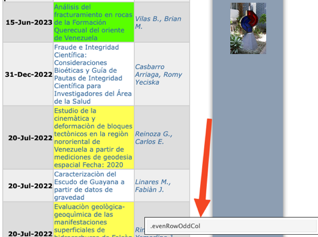
\includegraphics[width=0.5\linewidth]{images/05-desarrollo/1_ciclo/Picture3} 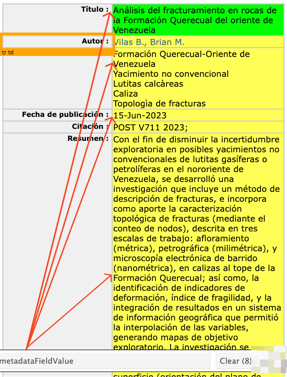
\includegraphics[width=0.5\linewidth]{images/05-desarrollo/1_ciclo/Picture2} 

}

\caption{Etiquetas nodos url´s}\label{fig:nodosurl}
\end{figure}

\begin{enumerate}
\def\labelenumi{\arabic{enumi}.}
\setcounter{enumi}{1}
\tightlist
\item
  En una segunda fase, mediante la misma técnica indicada en el punto anterior, se localizó en la ficha de un trabajo la etiqueta \emph{css}, en este caso la \emph{`.metadataFieldValue' ,} que está asociada al nodo que contiene los valores del: título, autor, fecha de publicación, palabras clave, url de descarga del documento y el texto del resumen. En la figura \ref{fig:nodosurl}-b se aprecia una imagen de una ficha. Al contar con el listado de url´s y la identificación de los datos a extraer, se hizo un bucle para visitar cada enlace, se descargó el archivo html, se accedió al nodo, se extrajeron los valores y se fueron almacenando en una estructura de datos.
\end{enumerate}

\hypertarget{aprender}{%
\paragraph{Aprender:}\label{aprender}}

Se enfrentaron las siguientes dificultades y se adoptaron en algunos casos las correspondientes soluciones:

\begin{enumerate}
\def\labelenumi{\arabic{enumi}.}
\item
  Se realizaron varios intentos para la descarga y extracción de los valores. Para la obtención de cada campo, en principio se tomó de referencia la posición fija en que aparecía dentro de la ficha, porque se había asumido que estas tenían la misma estructura para todos los trabajos, sin embargo en algunas aparecían otros valores, p.~ej. el de ``colección'', alterando la posición en que se encuentra el dato a extraer. La solución adoptada fue que primero se localizarán, dentro de cada ficha, los títulos de los campos, con esto se generó el listado de los valores posicionales y relativo a estos se extrajeron los valores propuestos.
\item
  Algunos valores de las fechas contenían información parcial faltando el mes y/o el día. Se adoptó un método de imputar el valor ``1'' tanto al mes como día faltante.
\item
  Adoptar previsiones para caídas del servidor de Saber UCV y resguardar en cada vuelta del bucle la información extraída, para no perder el trabajo de extracción acumulado en caso de una falla remota o local en el acceso.
\item
  La revisión del conjunto de datos obtenido mostró que existen 861 valores duplicados en el ``título'' de los trabajos. Esta situación también se presenta con un subconjunto distinto al anterior, donde existen ``resúmenes'' que están repetidos. Esto ocurre por la introducción de algún carácter adicional o mínimas alteraciones en el texto. Para descartar estos registros, se aplicó una función de limpieza al texto (convertir a minúscula, remover signos puntuación, etc.). Posteriormente se obtuvieron sendos valores \emph{hash} sobre el título y el resumen y luego se descartaron los \emph{hashes} duplicados. Adicionalmente se decidió usar el \emph{hash} obtenido del ``título procesado'' como el identificador único de cada documento. La remoción de investigaciones que puedan estar duplicadas es importante efectuarla, ya que al ejecutar los procesos de recuperación de información o la representación de los resultados en Mapas de Conocimiento, al incluir textos repetidos, creará representaciones distorsionadas. En el cuadro \ref{tab:cantidadesduplicados} se muestra la cantidad de los valores detectados por Jerarquía.
\end{enumerate}

\global\setlength{\Oldarrayrulewidth}{\arrayrulewidth}

\global\setlength{\Oldtabcolsep}{\tabcolsep}

\setlength{\tabcolsep}{0pt}

\renewcommand*{\arraystretch}{1.5}



\providecommand{\ascline}[3]{\noalign{\global\arrayrulewidth #1}\arrayrulecolor[HTML]{#2}\cline{#3}}

\begin{longtable}[c]{|p{1.07in}|p{1.25in}|p{0.89in}|p{1.21in}}

\caption{Cantidades\ de\ Trabajos\ Duplicados}\label{tab:cantidadesduplicados}\\

\ascline{1.5pt}{666666}{1-4}

\multicolumn{1}{>{\raggedright}m{\dimexpr 1.07in+0\tabcolsep}}{\textcolor[HTML]{000000}{\fontsize{11}{11}\selectfont{\global\setmainfont{Helvetica}{\textbf{Jerarquía}}}}} & \multicolumn{1}{>{\raggedleft}m{\dimexpr 1.25in+0\tabcolsep}}{\textcolor[HTML]{000000}{\fontsize{11}{11}\selectfont{\global\setmainfont{Helvetica}{\textbf{Disponibles}}}}} & \multicolumn{1}{>{\raggedleft}m{\dimexpr 0.89in+0\tabcolsep}}{\textcolor[HTML]{000000}{\fontsize{11}{11}\selectfont{\global\setmainfont{Helvetica}{\textbf{Únicos}}}}} & \multicolumn{1}{>{\raggedleft}m{\dimexpr 1.21in+0\tabcolsep}}{\textcolor[HTML]{000000}{\fontsize{11}{11}\selectfont{\global\setmainfont{Helvetica}{\textbf{Duplicados}}}}} \\

\ascline{1.5pt}{666666}{1-4}\endfirsthead \caption[]{Cantidades\ de\ Trabajos\ Duplicados}\label{tab:cantidadesduplicados}\\

\ascline{1.5pt}{666666}{1-4}

\multicolumn{1}{>{\raggedright}m{\dimexpr 1.07in+0\tabcolsep}}{\textcolor[HTML]{000000}{\fontsize{11}{11}\selectfont{\global\setmainfont{Helvetica}{\textbf{Jerarquía}}}}} & \multicolumn{1}{>{\raggedleft}m{\dimexpr 1.25in+0\tabcolsep}}{\textcolor[HTML]{000000}{\fontsize{11}{11}\selectfont{\global\setmainfont{Helvetica}{\textbf{Disponibles}}}}} & \multicolumn{1}{>{\raggedleft}m{\dimexpr 0.89in+0\tabcolsep}}{\textcolor[HTML]{000000}{\fontsize{11}{11}\selectfont{\global\setmainfont{Helvetica}{\textbf{Únicos}}}}} & \multicolumn{1}{>{\raggedleft}m{\dimexpr 1.21in+0\tabcolsep}}{\textcolor[HTML]{000000}{\fontsize{11}{11}\selectfont{\global\setmainfont{Helvetica}{\textbf{Duplicados}}}}} \\

\ascline{1.5pt}{666666}{1-4}\endhead



\multicolumn{4}{>{\raggedright}m{\dimexpr 4.43in+6\tabcolsep}}{\textcolor[HTML]{000000}{\fontsize{11}{11}\selectfont{\global\setmainfont{Helvetica}{cifras\ de\ Saber.UCV\ a\ la\ fecha\ 15/10/2023}}}} \\

\ascline{0.75pt}{666666}{1-4}\endfoot



\multicolumn{1}{>{\raggedright}m{\dimexpr 1.07in+0\tabcolsep}}{\textcolor[HTML]{000000}{\fontsize{11}{11}\selectfont{\global\setmainfont{Helvetica}{pregrado}}}} & \multicolumn{1}{>{\raggedleft}m{\dimexpr 1.25in+0\tabcolsep}}{\textcolor[HTML]{000000}{\fontsize{11}{11}\selectfont{\global\setmainfont{Helvetica}{8.305}}}} & \multicolumn{1}{>{\raggedleft}m{\dimexpr 0.89in+0\tabcolsep}}{\textcolor[HTML]{000000}{\fontsize{11}{11}\selectfont{\global\setmainfont{Helvetica}{7.634}}}} & \multicolumn{1}{>{\raggedleft}m{\dimexpr 1.21in+0\tabcolsep}}{\textcolor[HTML]{FF0000}{\fontsize{11}{11}\selectfont{\global\setmainfont{Helvetica}{671}}}} \\

\ascline{0.75pt}{666666}{1-4}



\multicolumn{1}{>{\raggedright}m{\dimexpr 1.07in+0\tabcolsep}}{\textcolor[HTML]{000000}{\fontsize{11}{11}\selectfont{\global\setmainfont{Helvetica}{otras}}}} & \multicolumn{1}{>{\raggedleft}m{\dimexpr 1.25in+0\tabcolsep}}{\textcolor[HTML]{000000}{\fontsize{11}{11}\selectfont{\global\setmainfont{Helvetica}{1.477}}}} & \multicolumn{1}{>{\raggedleft}m{\dimexpr 0.89in+0\tabcolsep}}{\textcolor[HTML]{000000}{\fontsize{11}{11}\selectfont{\global\setmainfont{Helvetica}{1.343}}}} & \multicolumn{1}{>{\raggedleft}m{\dimexpr 1.21in+0\tabcolsep}}{\textcolor[HTML]{FF0000}{\fontsize{11}{11}\selectfont{\global\setmainfont{Helvetica}{134}}}} \\

\ascline{0.75pt}{666666}{1-4}



\multicolumn{1}{>{\raggedright}m{\dimexpr 1.07in+0\tabcolsep}}{\textcolor[HTML]{000000}{\fontsize{11}{11}\selectfont{\global\setmainfont{Helvetica}{maestría}}}} & \multicolumn{1}{>{\raggedleft}m{\dimexpr 1.25in+0\tabcolsep}}{\textcolor[HTML]{000000}{\fontsize{11}{11}\selectfont{\global\setmainfont{Helvetica}{743}}}} & \multicolumn{1}{>{\raggedleft}m{\dimexpr 0.89in+0\tabcolsep}}{\textcolor[HTML]{000000}{\fontsize{11}{11}\selectfont{\global\setmainfont{Helvetica}{695}}}} & \multicolumn{1}{>{\raggedleft}m{\dimexpr 1.21in+0\tabcolsep}}{\textcolor[HTML]{FF0000}{\fontsize{11}{11}\selectfont{\global\setmainfont{Helvetica}{48}}}} \\

\ascline{0.75pt}{666666}{1-4}



\multicolumn{1}{>{\raggedright}m{\dimexpr 1.07in+0\tabcolsep}}{\textcolor[HTML]{000000}{\fontsize{11}{11}\selectfont{\global\setmainfont{Helvetica}{doctorado}}}} & \multicolumn{1}{>{\raggedleft}m{\dimexpr 1.25in+0\tabcolsep}}{\textcolor[HTML]{000000}{\fontsize{11}{11}\selectfont{\global\setmainfont{Helvetica}{318}}}} & \multicolumn{1}{>{\raggedleft}m{\dimexpr 0.89in+0\tabcolsep}}{\textcolor[HTML]{000000}{\fontsize{11}{11}\selectfont{\global\setmainfont{Helvetica}{310}}}} & \multicolumn{1}{>{\raggedleft}m{\dimexpr 1.21in+0\tabcolsep}}{\textcolor[HTML]{FF0000}{\fontsize{11}{11}\selectfont{\global\setmainfont{Helvetica}{8}}}} \\

\ascline{1.5pt}{666666}{1-4}



\end{longtable}



\arrayrulecolor[HTML]{000000}

\global\setlength{\arrayrulewidth}{\Oldarrayrulewidth}

\global\setlength{\tabcolsep}{\Oldtabcolsep}

\renewcommand*{\arraystretch}{1}

\hypertarget{labels}{%
\subsubsection{Iteración- Levantamiento de Categorías:}\label{labels}}

\hypertarget{especulaciuxf3n-2}{%
\paragraph{Especulación:}\label{especulaciuxf3n-2}}

Para poder clasificar cada investigación es necesario contar con las categorías que serán asignadas. Se entiende por ``categoría'' el nombre de la carrera de pregrado o el postgrado, junto con la facultad, que constituyen la oferta de la Universidad Central de Venezuela en educación universitaria.

Al no encontrarse el listado de categorías disponible en el propio repositorio Saber UCV fue necesario realizar una búsqueda web de esta información, extraerla y estructurarla, para así contar con el conjunto de datos de categorías que permita ejecutar la siguiente iteración, que es la de \textbf{Extracción y Clasificación de las Investigaciones} \ref{asignacion}.

\hypertarget{colaboraciuxf3n-2}{%
\paragraph{Colaboración:}\label{colaboraciuxf3n-2}}

Se visitó al sitio oficial de la Universidad Central de Venezuela para revisar la oferta de pregrados y postgrados. Para los postgrados se encontró para cada categoría (especialización, maestría y doctorado) una página con el listado, p.~ej. \href{http://www.ucv.ve/organizacion/vrac/gerencia-de-investigacion-cientifica-y-humanistica/gerencia-de-estudios-de-postgrado/programas-de-postgrado-ucv/maestria.html}{http://www.ucv.ve/organizacion/maestria.html} \footnote{previendo posibles modificacions en las páginas que contienen los listado de postgrados, se procedió a respaldarlas y forman parte del contenido del repositorio asociado a esta Investigación para garantizar la reproducibilidad de los resultados obtenidos. Para la fecha de redacción de este documento el contenido de los \emph{urls} indicados fue modificado}. En la figura \ref{fig:maestrias} se aprecian las potenciales etiquetas para las maestrías.

\begin{figure}

{\centering 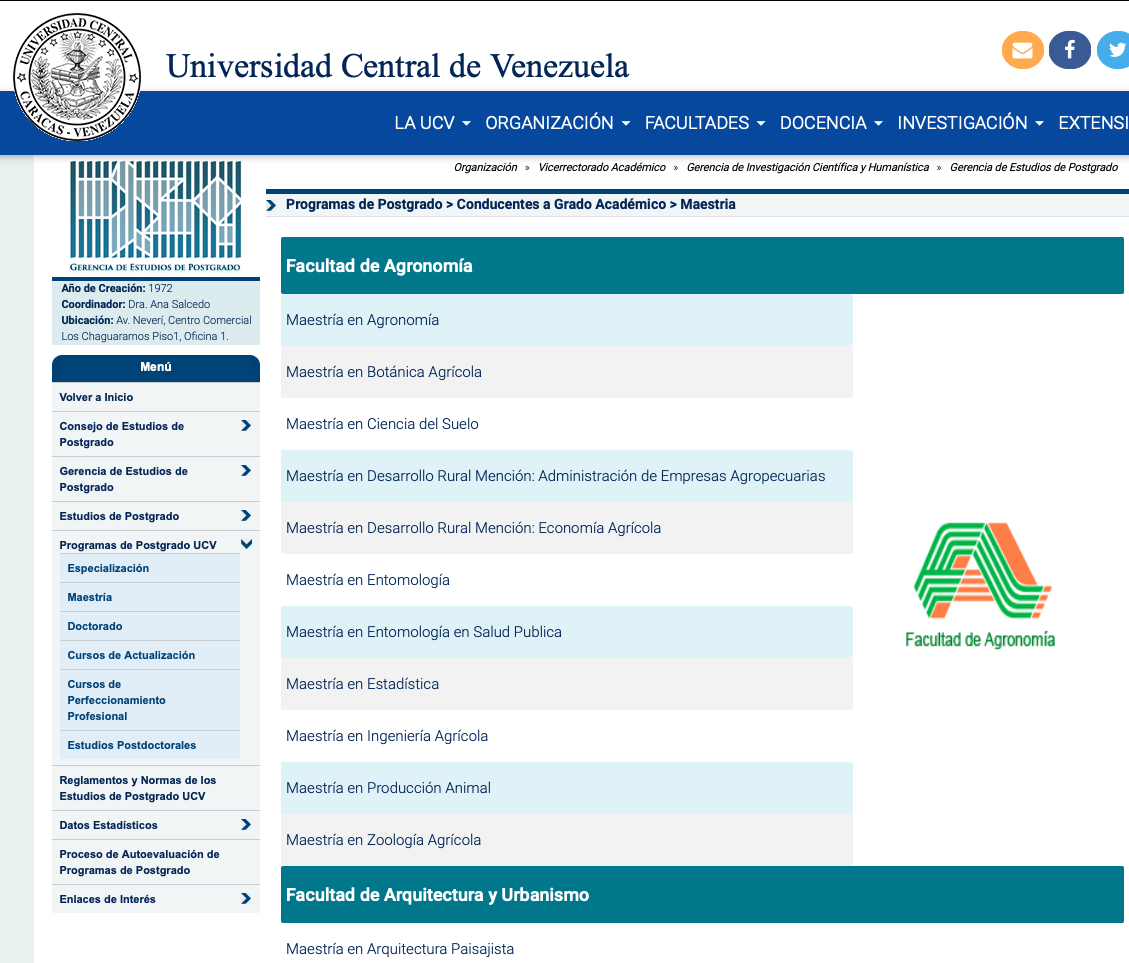
\includegraphics[width=0.4\linewidth]{images/05-desarrollo/1_ciclo/maestrias} 

}

\caption{Listado de Maestrías}\label{fig:maestrias}
\end{figure}

Mediante la técnica de recuperación de datos web la información descrita en \ref{scrapeo} se procedió a extraer el nombre de cada postgrado, añadir el nivel académico y asociar la facultad a la cual está adscrito. La cantidad de postgrados por nivel académico: Doctorado, Maetría y Especializaciones se muestran en el cuadro \ref{tab:resultpostgrado}.

\global\setlength{\Oldarrayrulewidth}{\arrayrulewidth}

\global\setlength{\Oldtabcolsep}{\tabcolsep}

\setlength{\tabcolsep}{0pt}

\renewcommand*{\arraystretch}{1.5}



\providecommand{\ascline}[3]{\noalign{\global\arrayrulewidth #1}\arrayrulecolor[HTML]{#2}\cline{#3}}

\begin{longtable}[c]{|p{1.15in}|p{1.01in}|p{1.52in}}

\caption{Cantidades\ de\ Postgrados\ por\ Categoría}\label{tab:resultpostgrado}\\

\ascline{1.5pt}{666666}{1-3}

\multicolumn{1}{>{\raggedleft}m{\dimexpr 1.15in+0\tabcolsep}}{\textcolor[HTML]{000000}{\fontsize{11}{11}\selectfont{\global\setmainfont{Helvetica}{\textbf{Doctorado}}}}} & \multicolumn{1}{>{\raggedleft}m{\dimexpr 1.01in+0\tabcolsep}}{\textcolor[HTML]{000000}{\fontsize{11}{11}\selectfont{\global\setmainfont{Helvetica}{\textbf{Maestría}}}}} & \multicolumn{1}{>{\raggedleft}m{\dimexpr 1.52in+0\tabcolsep}}{\textcolor[HTML]{000000}{\fontsize{11}{11}\selectfont{\global\setmainfont{Helvetica}{\textbf{Especialización}}}}} \\

\ascline{1.5pt}{666666}{1-3}\endfirsthead \caption[]{Cantidades\ de\ Postgrados\ por\ Categoría}\label{tab:resultpostgrado}\\

\ascline{1.5pt}{666666}{1-3}

\multicolumn{1}{>{\raggedleft}m{\dimexpr 1.15in+0\tabcolsep}}{\textcolor[HTML]{000000}{\fontsize{11}{11}\selectfont{\global\setmainfont{Helvetica}{\textbf{Doctorado}}}}} & \multicolumn{1}{>{\raggedleft}m{\dimexpr 1.01in+0\tabcolsep}}{\textcolor[HTML]{000000}{\fontsize{11}{11}\selectfont{\global\setmainfont{Helvetica}{\textbf{Maestría}}}}} & \multicolumn{1}{>{\raggedleft}m{\dimexpr 1.52in+0\tabcolsep}}{\textcolor[HTML]{000000}{\fontsize{11}{11}\selectfont{\global\setmainfont{Helvetica}{\textbf{Especialización}}}}} \\

\ascline{1.5pt}{666666}{1-3}\endhead



\multicolumn{1}{>{\raggedleft}m{\dimexpr 1.15in+0\tabcolsep}}{\textcolor[HTML]{000000}{\fontsize{11}{11}\selectfont{\global\setmainfont{Helvetica}{46}}}} & \multicolumn{1}{>{\raggedleft}m{\dimexpr 1.01in+0\tabcolsep}}{\textcolor[HTML]{000000}{\fontsize{11}{11}\selectfont{\global\setmainfont{Helvetica}{101}}}} & \multicolumn{1}{>{\raggedleft}m{\dimexpr 1.52in+0\tabcolsep}}{\textcolor[HTML]{000000}{\fontsize{11}{11}\selectfont{\global\setmainfont{Helvetica}{228}}}} \\

\ascline{1.5pt}{666666}{1-3}



\end{longtable}



\arrayrulecolor[HTML]{000000}

\global\setlength{\arrayrulewidth}{\Oldarrayrulewidth}

\global\setlength{\tabcolsep}{\Oldtabcolsep}

\renewcommand*{\arraystretch}{1}

En cuanto a los pregrados no se encontró en el sitio de la Universidad en una página centralizada la información y se procedió a obtenerla de la página \href{https://es.wikipedia.org/wiki/Anexo:Facultades_de_la_Universidad_Central_de_Venezuela}{wikipedia} asociada a la U.C.V. recuperando un total del 50 nombres de escuelas de pregrado junto con la facultad de dependencia.

En la figura \ref{fig:jerarquias} se muestran los totales apilados de pregrados y postgrados que se encontraron por Facultad-Centro de Investigación durante el levantamiento de información, cifra que al totalizar los postgrados y pregrados alcanza la cantidad de 425 áreas de conocimiento.

\begin{figure}
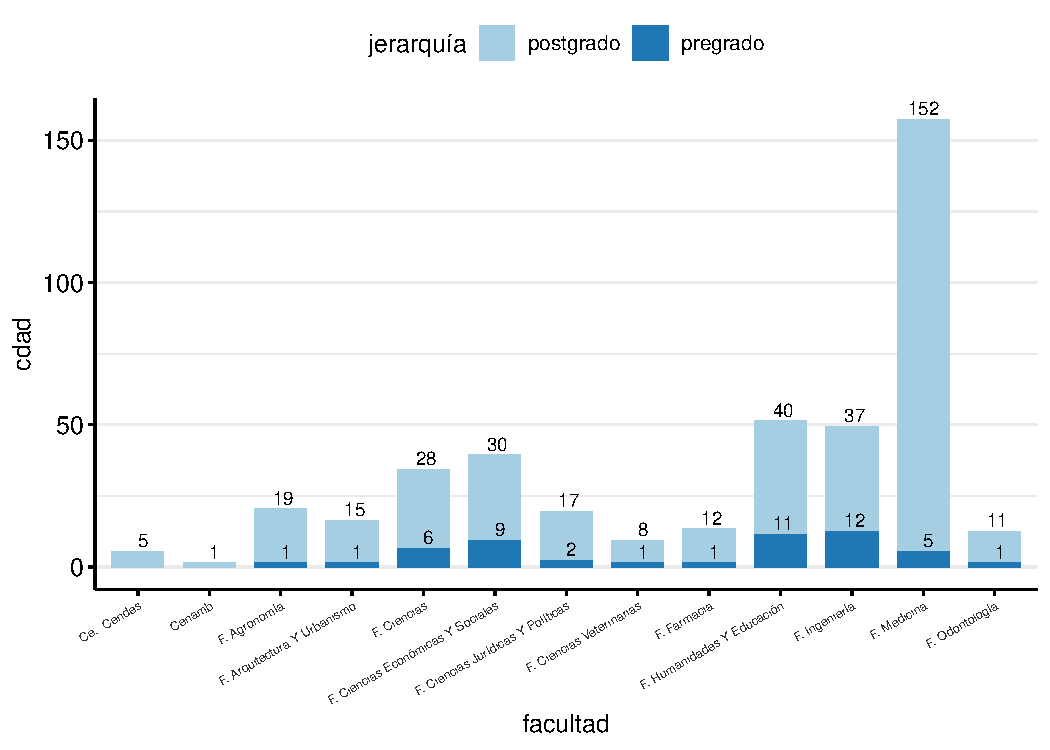
\includegraphics[width=0.7\linewidth]{_main_files/figure-latex/jerarquias-1} \caption{Total pregrados y postgrados por Facultad-Centro}\label{fig:jerarquias}
\end{figure}

\hypertarget{aprender-1}{%
\paragraph{Aprender:}\label{aprender-1}}

\begin{enumerate}
\def\labelenumi{\arabic{enumi}.}
\item
  En el caso de los postgrados, inicialmente se esperaba que sólo estuvieran asociados a Facultades pero también se encontró que el Centro de Estudios del Desarrollo y el Centro de Estudios Integrales del Ambiente imparten este tipo de estudios.
\item
  Se evaluó que existen nombres postgrados duplicados con la misma categoría, lo que puede generar problemas en la clasificación de las investigaciones teniendo como ejemplo la ``Maestría en Estadística'' que se dicta en la Facultad de Agronomía y en la Facultad de Ciencias Económicas y Sociales.
\item
  Se detectó que en pregrado existen escuelas que otorgan distintos títulos, p.~ej. de la ``Escuela de Administración y Contaduría'' se pueden obtener los títulos de ``contador'' o de ``licenciado en administración''. Esto es algo a tener presente al momento de hacer la categorización, ya que el nombre de la escuela no sirve en estos casos para realizarla, siendo necesario agregar al conjunto de datos el atributo del nombre de los títulos emitidos.
\item
  Sobre los textos se tuvieron que realizar modificaciones, ya que en los listados se encontró que algunos nombres les faltaban palabras. La revisión final de nombres, dada la cantidad total de 425 dependencias, se hizo manualmente para evitar posteriores categorizaciones erróneas .
\end{enumerate}

\hypertarget{asignacion}{%
\subsubsection{Iteración- Extracción y Clasificación de las Investigaciones:}\label{asignacion}}

En esta iteración se mencionan los principales obstáculos y las estrategias implementadas para alcanzar el objetivo de realizar la clasificación de cada trabajo alojado en Saber UCV, no obstante se omite especificar algunos de los problemas que se encontraron, ya que extenderse en esto abultaría considerablemente el contenido expuesto.

\hypertarget{especulaciuxf3n-3}{%
\paragraph{Especulación:}\label{especulaciuxf3n-3}}

Para las investigaciones que reposan en Saber UCV que cuentan con un archivo anexo, correspondiente al documento de la misma, es posible realizar la descarga, extraer una porción de texto y adoptando métodos basados en reglas de coincidencia de patrones, con las etiquetas obtenidas en la iteración \ref{labels} \textbf{Levantamiento de Categorías}, hacer la categorización por área de estudio, asignando el nombre del pre o postgrado, la escuela-postgrado y la facultad-centro de adscripción. Igualmente de esta porción de texto se estima viable extraer el nombre del tutor.

\hypertarget{colaboraciuxf3n-3}{%
\paragraph{Colaboración:}\label{colaboraciuxf3n-3}}

Motivado a que en la primera iteración \ref{scrapeo} para conformar el conjunto de datos se había obtenido el \emph{url} asociado al documento soporte de la investigación, se procedió mediante un bucle a realizar la descarga de cada documento y extraer una cantidad de dos mil caracteres, partiendo del principio de que los trabajos de grado o tesis en sus primeras páginas tienen el nombre de la carrera o el postgrado, el nombre de la facultad-centro donde se cursó el estudio, el nombre del título al que optan y el nombre del tutor.

En esta iteración fue necesario realizar distintas adaptaciones para lograr la coincidencia de patrones. Teniendo en cuenta que son 425 etiquetas las que se usarán para realizar la clasificación, llegando a tener 14 palabras algunas categorías, es elevada la probabilidad de que no se pueda hacer el ``\emph{pattern matching}'' entre el texto y la etiqueta.

Lo anterior motivo a realizar un proceso de limpieza, modificación y disminución de la cantidad de palabras, tanto en las etiquetas como en el texto extraído. Se evaluó en cada adaptación cuáles razones impedían clasificar los documentos aún pendientes, se tomaron los correctivos y así se fue incrementando, de forma iterativa, la precisión en este proceso.

También se tuvo que tomar en cuenta el orden en que se iba a ejecutar la secuencia de encontrar las coincidencias. Ejemplo es que varias facultades contienen las mismas tres palabras en la parte inicial de su nombre: \emph{Facultad de Ciencias}, \emph{Facultad de Ciencias} Jurídicas y Políticas, \emph{Facultad de Ciencias} Económicas y Sociales y la \emph{Facultad de Ciencias} Veterinarias. La secuencia para hacer la detección de la coincidencia fue buscar en orden decreciente por el total de caracteres que tenga el nombre de la facultad, para evitar clasificaciones erróneas.

Adicionalmente en el proceso de hacer coincidir las frases, se encontraron 17 postgrados que no estaban en el listado previamente conformado, los cuales se tuvieron que agregar al conjunto de datos de las categorías.

Para aquellos casos donde no se podía hacer \emph{match} se aplicó el algorimo ``Smith Waterman'' \citep{smith1981}, expuesto en el Capítulo del Marco Teórico \ref{alghist}, el cual permite alinear dos cadenas de texto cuando una de ellas no tiene coincidencia absoluta con la otra, como puede pasar en este caso por la introducción de caracteres adicionales.

Un elemento que introdujo ruido en el texto leído de los documentos, fue la aparición de diversos \emph{encodings} que no resultó viable codificarlos a ``UTF-08'', haciendo que aparecieran caracteres no reconocidos dentro del texto, dificultando la tarea de lograr realizar el proceso de ``pattern matching''. El algorimo SW resultó eficaz para solucionar este problema, aunque igualmente se hicieron pruebas con otros métodos como el algoritmo de ``Distancia de Levenshtein'' o similares.

Sobre un total de 9.982 potenciales documentos se lograron clasificar 9.585 investigaciones, mientras que 244 no disponían información en el texto del documento y resultaba inviable hacer la categorización. En algunos casos esta falta de información estuvo motivada en que el archivo contenía imágenes por estar escaneado el contenido o los documentos anexos no eran trabajos de grado o tesis sino informes de algún otro estilo.

La cantidad de categorías distintas, con al menos una investigación asignada a una facultad o centro, ascendió a 284 que se distribuyen por Facultad según lo que se observa en la figura \ref{fig:categorias}

\begin{figure}
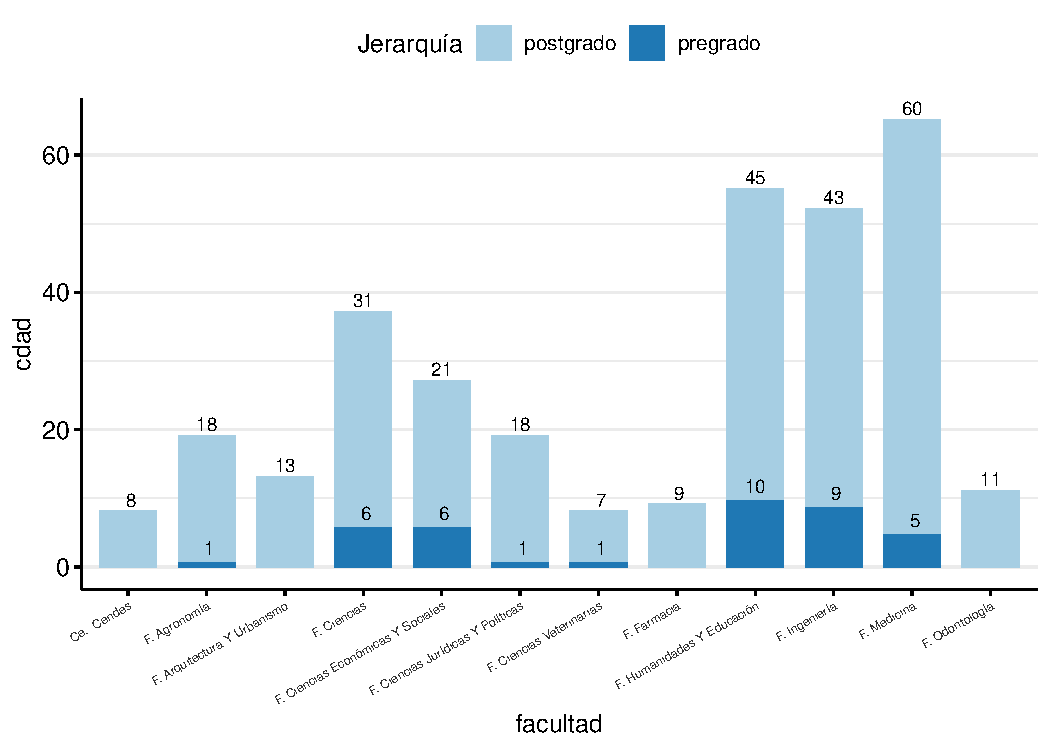
\includegraphics[width=0.7\linewidth]{_main_files/figure-latex/categorias-1} \caption{Cantidades de categorías por facultad y nivel académico}\label{fig:categorias}
\end{figure}

En en la figura \ref{fig:totalesporfacultad} se pueden ver primero la cantidad total de investigaciones que pudieron ser clasificadas por cada Facultad - Centro de estudios y en la segunda posición, la cantidad de documentos disponibles por fecha de publicación que abarcan el período 01/01/1977 al 06/15/2023.

\begin{figure}
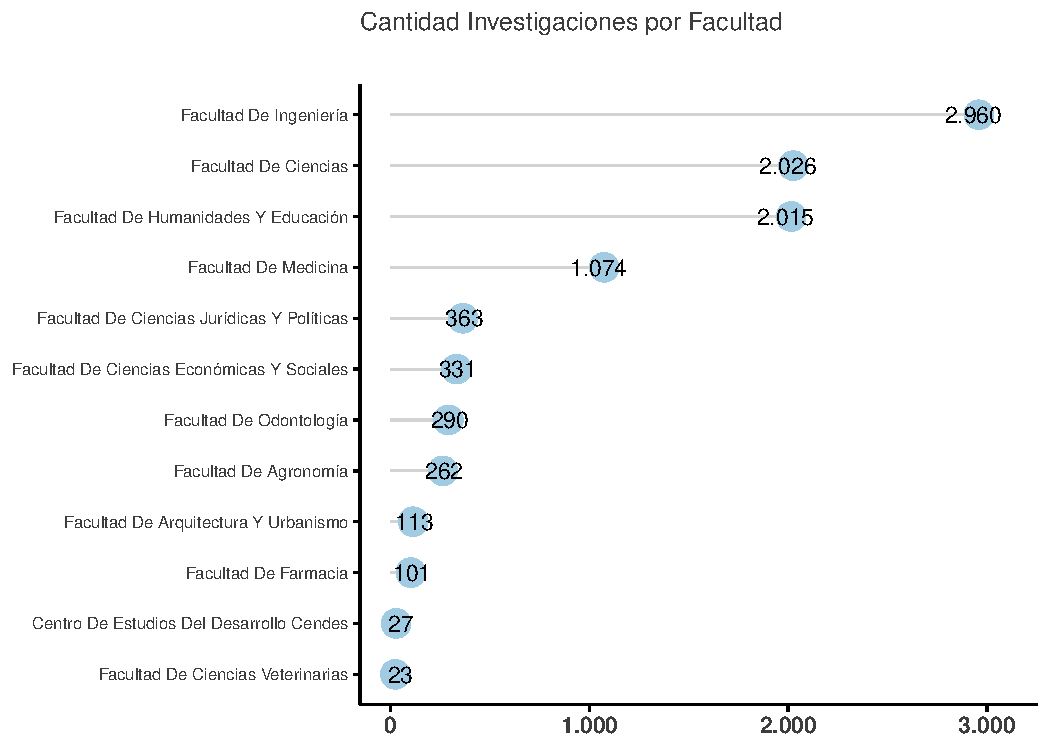
\includegraphics[width=0.45\linewidth]{_main_files/figure-latex/totalesporfacultad-1} 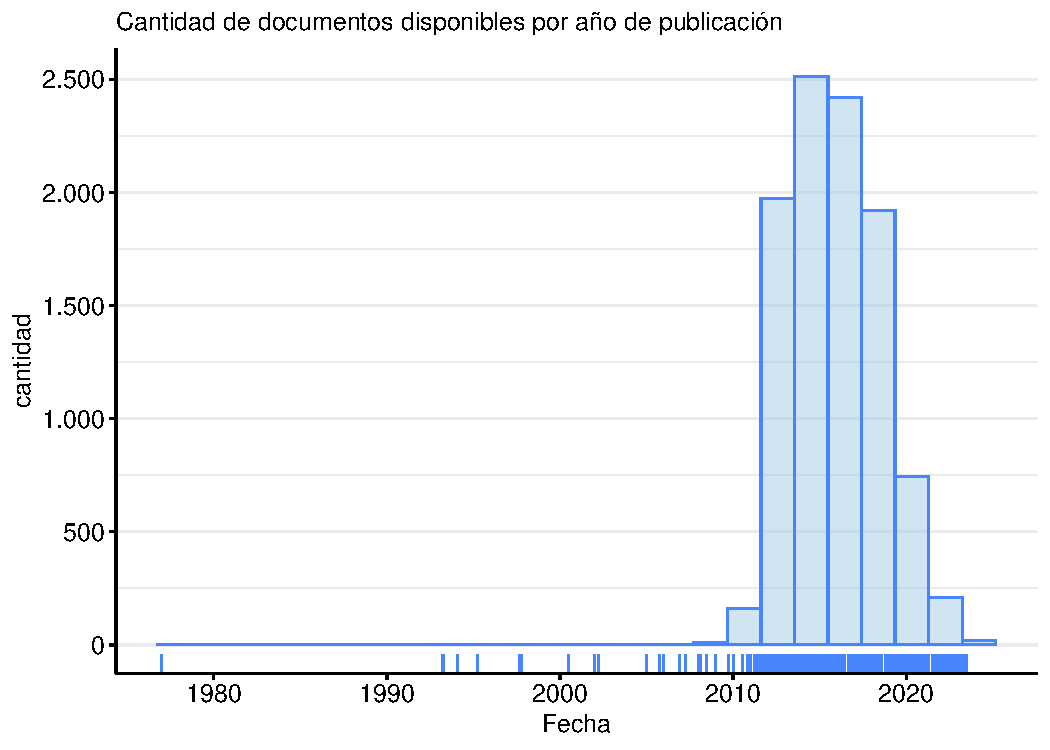
\includegraphics[width=0.45\linewidth]{_main_files/figure-latex/totalesporfacultad-2} \caption{Cantidades de investigaciones clasificadas por Facultad y por año de publicación}\label{fig:totalesporfacultad}
\end{figure}

En cuanto a la obtención de los nombres de los tutores, el procedimiento adoptado fue nuevamente realizar algunas limpiezas sobre el texto como remover digitos, abreviaturas de títulos académicos ( PhD, MgS, etc), y luego extraer el texto que se encontraba delimitado entre la propia palabra ``tutor'' y el brinco de línea ``\textbackslash n'' más próximo a la aparición de dicha palabra. Con el procedimiento descrito se pudo extraer un total de 7.969 nombres, equivalente al 79,8\% de las investigaciones, así como 3.718 nombres únicos. En la figura \ref{fig:tutores} se aprecia la frecuencia para la cantidad de investigaciones que corresponden a un mismo tutor.

\begin{figure}
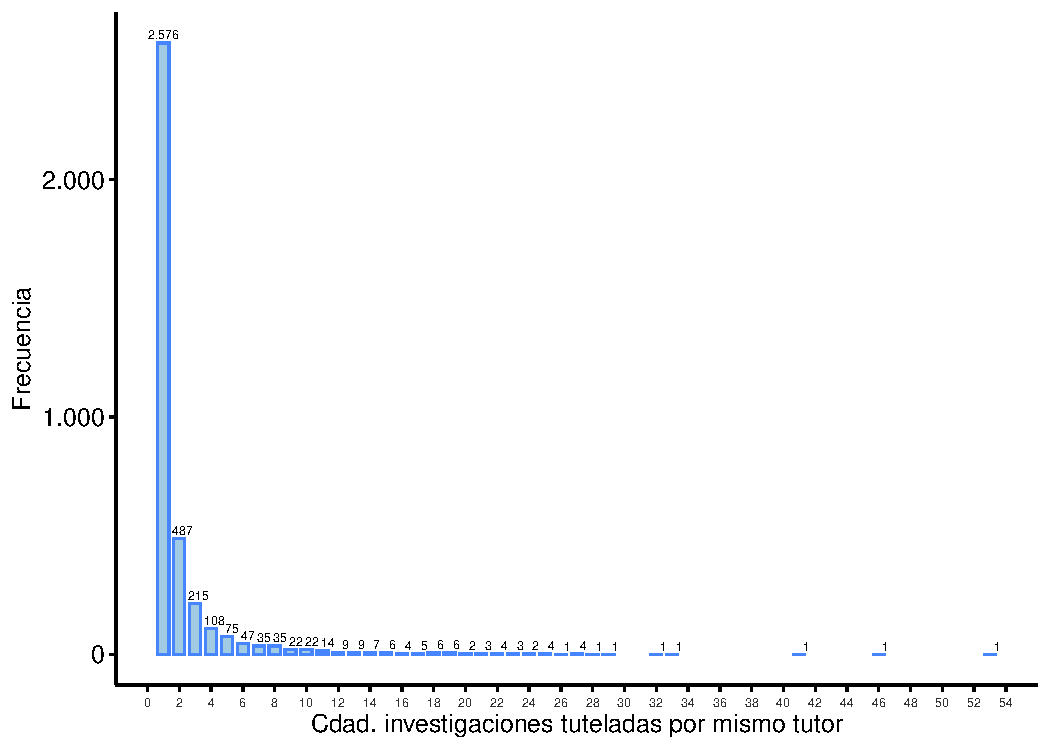
\includegraphics[width=0.65\linewidth]{_main_files/figure-latex/tutores-1} \caption{Histógrama Nombres Tutores Extraídos }\label{fig:tutores}
\end{figure}

La cantidad de trabajos donde fue detectado que un tutor tuvo dos o más trabajos tutelados es 5.393, equivalente a un 54\%. La cifra anterior tiene la significancia de mostrar que para más de la mitad de los trabajos existe la certeza de que se encontró un nombre idéntico, en al menos dos casos, brindando mayor confianza sobre el proceso ejecutado.

En los otros 2.576 casos, en que sólo se encontró un tutor por investigación, al realizar un análisis exploratorio, se pudo apreciar que en una variedad de casos el nombre no fue escrito en forma idéntica entre un trabajo y otro, p.~ej. dejando unicamente la inicial del segundo apellido u omitiendo el segundo nombre. Escapa al alcance de este trabajo realizar la depuración que permita consolidar más trabajos de grado al correspondiente tutor.

\hypertarget{aprender-2}{%
\paragraph{Aprender:}\label{aprender-2}}

A continuación se agrupan y enuncian los principales inconvenientes que se encontraron y se indica el aprendizaje obtenido para fases sucesivas de desarrollo:

\begin{enumerate}
\def\labelenumi{\arabic{enumi}.}
\item
  Aparición de errores en la redacción y ortográfia por parte de los autores, como por ejemplo, escribir incorrectamente el nombre del título al que optan o la facultad donde realizaron los estudios. Esto implicó crear reglas para realizar reemplazos de palabras en los textos y limpiezas para disminuir el ruido y facilitar el proceso de obtener la coincidencia. Un problema que se presentaría al intentar extender el SCSU a otros repositorios, cuando los trabajos de grado no estén categorizados, es que el procedimiento anterior no es completamente generalizable si los nombres de los postgrados-escuelas y el de las facultades son distintos, ya que las reglas de modificación de texto son específicas para el corpus de la Universidad Central de Venezuela.
\item
  Cambios en el estilo y formalidades con que se deben presentar los documentos de grado en las distintas facultades o niveles académicos, cuestión que dificultó la detección de las reglas para hacer la comparación. Ante esto se buscó encontrar las formas más genéricas en el procesamiento, así como la adopción de un procedimiento que progresivamente intentaba obtener la coindicidencia: primero con el nombre del título, en caso de fallo se sigue con el nombre del pregrado o postgrado, si nuevamente fallaba se procedía a hacer la búsqueda del nombre de la facultad y finalmente si ninguna de las estrategias anteriores tenía éxito, se aplicaba el algoritmo ``Smith Waterman'', con el cual se pudieron clasificar 1.658 trabajos, que equivalen a un 16,6\% del total. Es importante señalar que al aplicar este último recurso se pueden generar ``falsos positivos'' y por esto en la Sección \ref{pruebas} se hace una estimación estadística del error que puede representar acudir a este método.
\item
  Dentro de los archivos descargados se encontraron algunos en formato de presentaciones \emph{power point} los cuales fueron desechados sólo siendo procesados los que estuviesen en formato \emph{word} o \emph{pdf} . Esto llevo a condicionar posteriormente que para ejecutar la descarga y hacer el procesamiento de extracción de datos, la extensión debía alguna de las mencionadas como válidas\emph{.}
\item
  También se encontraron trabajos que contaban con más de un archivo disponible para descargar. En la fase inicial se descargaron 12.765 de documentos aunque la cantidad de trabajos disponibles en el repositorio (incluyendo duplicados) era 10.843. Al evaluar las razones que motivaban que existiera una cantidad superior de archivos vs.~documentos, se encontraron casos en que por investigación existía un archivo por capítulo y no se encontraba algún elemento que indicará la secuencia en que se debía cargar cada archivo para armar el documento unificado. Para estos casos sólo se tomó el primer archivo en la lista de \emph{url}´s disponibles para tratar de hacer el proceso de clasificación.
\item
  Se hicieron algunas simplificaciones sobre postgrados que dependen de dos facultades imputándolo sólo a una que fuese la primera en aparecer en el texto. Como queda fuera del alcance de esta Investigación determinar los casos en que existen este tipo de adscripciones compartidas se hizo esta simplificación \footnote{Un ejemplo de esto es la Maestría en Física Médica que es impartida de manera conjunta por la Facultad de Ciencias y por la Facultad de Medicina. Al no disponer de información oficial sobre otros casos de postrgrados que presenten esta característica, se adoptó el método mencionado de imputar sólo a una dependencia que sea la primera en aparecer en el texto.}.
\item
  Algunos trabajos en su primera página incluyen el nombre de dos facultades o escuelas creando errores en la clasificación. P. ej., investigaciones que indican en la portada el siguiente texto ``Facultad de Ciencias, Escuela de Computación, título: se realiza la propuesta de un sistema de gestión académica para la Escuela de Economía de la Facultad de Ciencias Económicas\ldots.'', lo cual genera mútilples clasificaciones. En estos casos se optó por realizar la imputación con base en la primera coincidencia detectada.
\item
  En la obtención del nombre del tutor es importante destacar que en varios casos el texto extraído no se corresponde propiamente al nombre del mismo, motivado a que la escritura de la portada puede responder a la representación visual. Se encontraron trabajos que tienen tutor académico, tutor industrial, cotutor y otras variantes, donde se hace una disposición en la escritura de colocar el tipo de cada tutor alíneado cada uno en los extremos de una línea y los nombres también se disponen en los extremos de la línea superior, quebrando la regla de extracción que se había diseñando. Esto pareciera un problema a enfrentar con técnicas de segmentación de archivos que tienen en consideración la disposición visual. En el caso de esta investigación no se adoptaron métodos para abordar este problema. En las Sección \ref{pruebas} se hace una evaluación estadística de la precisión alcanzada en esta extracción.
\item
  Se simplificaron algunos nombres de especializaciones por la cantidad de palabras que tienen estableciendo un límite, o \emph{prunning}, de 5 palabras para el nombre del postgrado, lo que implica que algunos trabajos habrán quedado agrupados en la misma categoría. Estos casos mayormente están asociados a las especializaciones en el área de medicina, teniendo de ejemplo la figura \ref{fig:especial}.

  \begin{figure}

  {\centering 
\includegraphics[width=0.5\linewidth]{images/05-desarrollo/1_ciclo/especializaciones2} 

  }

  \caption{Ejemplo de nombres simplificados}\label{fig:especial}
  \end{figure}
\item
  En este proceso de clasificación no resultaba conveniente usar técnicas de aprendizaje automático dada la cantidad de categorías y el gran desbalanceo de clases.
\item
  Se detectó que en Saber UCV en la categoría que se denomina ``otros'' en Saber UCV se encuentran documentos que corresponden a especializaciones y también 60 trabajos de ascenso de profesores.
\end{enumerate}

\hypertarget{objetivos-alcanzados}{%
\subsubsection{Objetivos alcanzados:}\label{objetivos-alcanzados}}

\begin{enumerate}
\def\labelenumi{\arabic{enumi}.}
\item
  Obtener las fichas de 9.982 investigaciones, equivalente al 100\% de los trabajos de pre y postgrado alojados en Saber UCV (descartando los duplicados) , conforme a lo propuesto en el Objetivo Específico 1.
\item
  Obtener 375 nombres de postgrado y 50 de carreras de pregrado, insumo necesario para alcanzar lo propuesto en el Objetivo Específico 2.
\item
  Categorizar 9.585 investigaciones por área académica, equivalente al 96\% de toda la información a clasificar, de acuerdo al Objetivo Específico 2.
\item
  Extraer 7.969 nombres de tutores, equivalente al 79,8\% del total de investigaciones, que también se estableció como parte del Objetivo Específico 2.
\end{enumerate}

\newpage

\hypertarget{desarrollociclos3}{%
\subsection{Ciclo-Prototipo del SCSU:}\label{desarrollociclos3}}

En este ciclo se desarrolló el \textbf{Prototipo del Sistema Complementario Saber UCV} con tres iteraciones. En la primera iteración de este ciclo \ref{iternlp} se realizó la \textbf{Preparación del Corpus}. En la segunda iteración se hicieron las pruebas para realizar las \textbf{Recomendaciones} de cada documento, basado en la similitud que presente con el resto de las investigaciones. En la tercera \ref{imrecomendacion} \ref{iterbol} se creó una aplicación web interactiva en la que se implementó el \textbf{Prototipo} donde ante un \emph{query} se presentan los resultados y la visualización de los \textbf{``Mapa de Conocimiento''} (ver \ref{mapacon}) .

Todo las rutinas y codificaciones que se mencionan a continuación fueron realizadas en el lenguaje R version 4.3.2 (2023-10-31) \citep{R}.

\hypertarget{iternlp}{%
\subsubsection{Iteración- Preparación del Corpus:}\label{iternlp}}

En esta iteración el Corpus que se conformó en \ref{desarrollociclos1}, fue sometido a distintos procesamientos conocidos como ``Preparación del Corpus'' mediante la aplicación de técnicas de PLN, ver \ref{nlproc}. .

\hypertarget{especulaciuxf3n-4}{%
\paragraph{Especulación:}\label{especulaciuxf3n-4}}

Creando un corpus anotado con métodos del Procesamiento del Lenguaje Natural se facilita el acceso a información de relevancia para los investigadores mediante el análisis lingüístico de los documentos recolectados \citep{article}.

\hypertarget{colaboraciuxf3n-4}{%
\paragraph{Colaboración:}\label{colaboraciuxf3n-4}}

Para realizar el etiquetado de la ``Parte del Discurso (POS)'' \ref{pos}, se hizo una revisión exhaustiva de distintos \emph{frameworks} para realizar el anotado del Corpus, como \emph{Freeling} \citep{padro12}, CoreNLP \citep{manning-etal-2014-stanford}, UDPIPE \citep{udpipe-2} y se decidió acudir a la librería ``spacyr'' \citep{spacyr} que es un \emph{wrapper} de la librería Spacy \citep{spacy2020}, que se ejecuta en el lenguaje python. Esta librería, en lo relativo al etiquetado de las palabras por su función gramátical, lo hace acorde al marco de trabajo propuesto en la investigación ``Universal Dependencies'' \citep{demarneffe2021}. La implementación de \emph{Spacy} dispone de un encadenamiento en el flujo de trabajo, resultando conveniente aplicarlo dentro del desarrollo del SCSU. Otra de las características que dispone es contar con varios modelos preentrenados para realizar el etiquetado, así como disponer de métricas de desempeño que se encuentran dentro del estado del arte en el campo del Procesamiento del Lenguaje Natural.

La librería carga el modelo preentrenado de aprendizaje automático para el idioma español denominado ``es\_core\_news\_lg''. Mediante un \emph{pipeline} que se observa en la figura \ref{fig:spacypi} se ejecutan procesos que permiten conformar el Corpus Anotado.

\begin{figure}

{\centering 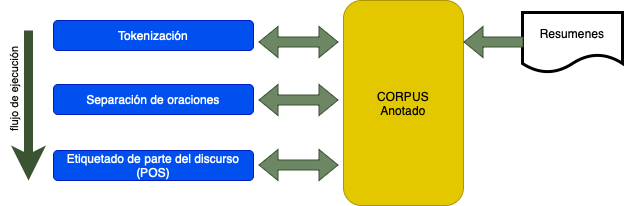
\includegraphics[width=0.8\linewidth]{images/05-desarrollo/2_ciclo/nlp/spacy_pipeline1} 

}

\caption{Arquitectura General pipeline Spacy}\label{fig:spacypi}
\end{figure}

Ilustrativamente se muestra el texto ``\emph{\ldots{} y algunos no-metales. Contrariamente a lo\ldots{}}'', que al aplicar los métodos que dispone ``spacyr'', permite generar el Corpus Anotado que se puede ver en la figura \ref{fig:corpusano}, donde se aprecia:

\begin{itemize}
\item
  id del documento
\item
  id de la oración dentro del documento
\item
  id del token dentro del documento
\item
  token
\item
  lema
\item
  etiquetado de parte del discurso (POS) para cada token.
\end{itemize}

\begin{figure}

{\centering 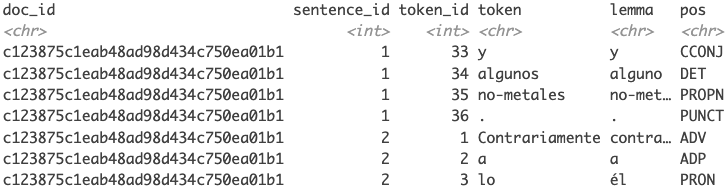
\includegraphics[width=0.9\linewidth]{images/05-desarrollo/2_ciclo/nlp/corpusanotado2} 

}

\caption{Detalle anotación del Corpus}\label{fig:corpusano}
\end{figure}

El Corpus Anotado cuenta con 9.982 documentos que generan 3.147.740 tokens, un vocabulario de 101.066 palabras distintas y 83.402 lemas únicos. Los tokens, agrupados por función gramatical se presentan \footnote{El proyecto Universal Dependencies disponible en el enlace \url{https://universaldependencies.org} contiene la documentación sobre las distintas funciones gramaticales que fueron etiquetadas.} en el gráfico \ref{fig:posgr} :

\begin{figure}

{\centering 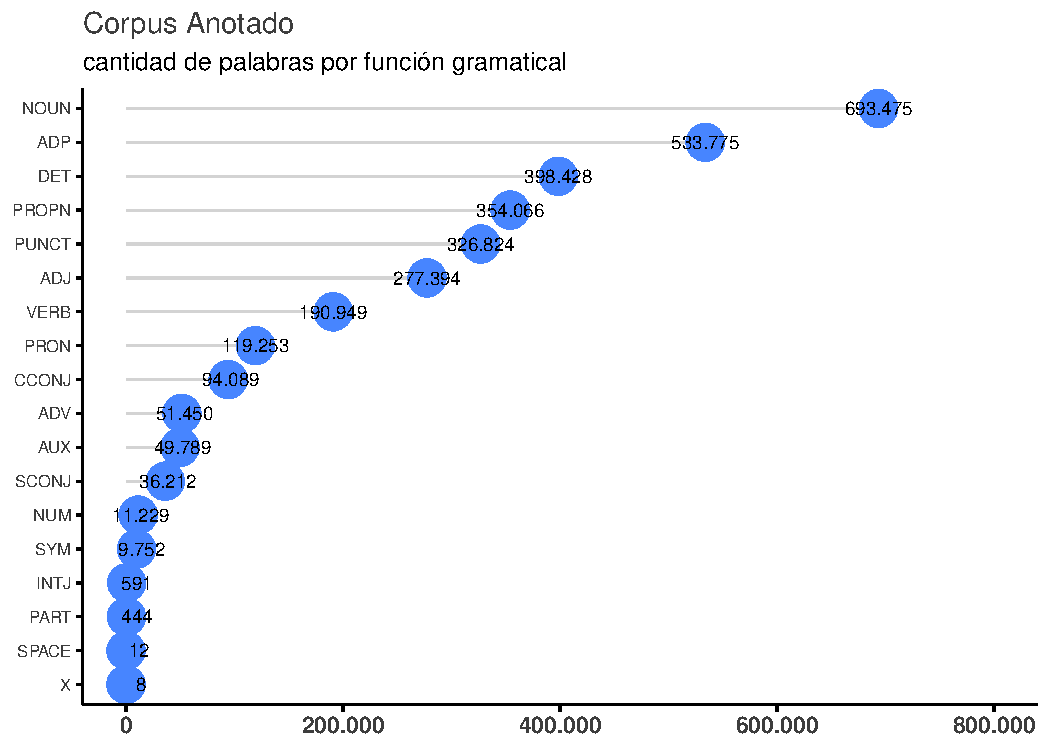
\includegraphics[width=0.7\linewidth]{_main_files/figure-latex/posgr-1} 

}

\caption{Cantidad de palabras por función gramatical}\label{fig:posgr}
\end{figure}

Realizando el análisis exploratorio del Corpus, es interesante ver la cantidad de palabras únicas por función gramatical y el ratio que presentan con respecto al total de palabras por ``POS'' que se vio en la figura \ref{fig:posgr}. En la tabla \ref{tab:lemmasg} se observa que las categorías del ``etiquetado de la parte del discurso'' que contienen mayor cantidad de información son los nombres propios (PROPN), los adjetivos (ADJ), números (NUM) y los sustantivos (NOUN), pero los nombres propios al ser únicos en cada trabajo y los números represetar cantidades, realmente la mayor cantidad de información del Corpus se encuentra en los adjetivos y sustantivos, lo que refuerza la construcción y representación de los Mapas de Conocimiento mediante la selección de las palabras que tienen las funciones gramatical de sustantivos y adjetivos, al presentar la mejor relación señal/ruido.

\global\setlength{\Oldarrayrulewidth}{\arrayrulewidth}

\global\setlength{\Oldtabcolsep}{\tabcolsep}

\setlength{\tabcolsep}{0pt}

\renewcommand*{\arraystretch}{1.5}



\providecommand{\ascline}[3]{\noalign{\global\arrayrulewidth #1}\arrayrulecolor[HTML]{#2}\cline{#3}}

\begin{longtable}[c]{|p{0.93in}|p{1.04in}|p{1.34in}|p{0.77in}}

\caption{Ratio\ de\ Cantidad\ Única\ de\ lemas\ Vs.\ Cantidad\ total\ de\ lemas}\label{tab:lemmasg}\\

\ascline{1.5pt}{666666}{1-4}

\multicolumn{1}{>{\raggedright}m{\dimexpr 0.93in+0\tabcolsep}}{\textcolor[HTML]{000000}{\fontsize{11}{11}\selectfont{\global\setmainfont{Helvetica}{\textbf{POS}}}}} & \multicolumn{1}{>{\raggedleft}m{\dimexpr 1.04in+0\tabcolsep}}{\textcolor[HTML]{000000}{\fontsize{11}{11}\selectfont{\global\setmainfont{Helvetica}{\textbf{Cantidad}}}}} & \multicolumn{1}{>{\raggedleft}m{\dimexpr 1.34in+0\tabcolsep}}{\textcolor[HTML]{000000}{\fontsize{11}{11}\selectfont{\global\setmainfont{Helvetica}{\textbf{Cdad.\ únicas}}}}} & \multicolumn{1}{>{\raggedleft}m{\dimexpr 0.77in+0\tabcolsep}}{\textcolor[HTML]{000000}{\fontsize{11}{11}\selectfont{\global\setmainfont{Helvetica}{\textbf{ratio}}}}} \\

\ascline{1.5pt}{666666}{1-4}\endfirsthead \caption[]{Ratio\ de\ Cantidad\ Única\ de\ lemas\ Vs.\ Cantidad\ total\ de\ lemas}\label{tab:lemmasg}\\

\ascline{1.5pt}{666666}{1-4}

\multicolumn{1}{>{\raggedright}m{\dimexpr 0.93in+0\tabcolsep}}{\textcolor[HTML]{000000}{\fontsize{11}{11}\selectfont{\global\setmainfont{Helvetica}{\textbf{POS}}}}} & \multicolumn{1}{>{\raggedleft}m{\dimexpr 1.04in+0\tabcolsep}}{\textcolor[HTML]{000000}{\fontsize{11}{11}\selectfont{\global\setmainfont{Helvetica}{\textbf{Cantidad}}}}} & \multicolumn{1}{>{\raggedleft}m{\dimexpr 1.34in+0\tabcolsep}}{\textcolor[HTML]{000000}{\fontsize{11}{11}\selectfont{\global\setmainfont{Helvetica}{\textbf{Cdad.\ únicas}}}}} & \multicolumn{1}{>{\raggedleft}m{\dimexpr 0.77in+0\tabcolsep}}{\textcolor[HTML]{000000}{\fontsize{11}{11}\selectfont{\global\setmainfont{Helvetica}{\textbf{ratio}}}}} \\

\ascline{1.5pt}{666666}{1-4}\endhead



\multicolumn{1}{>{\raggedright}m{\dimexpr 0.93in+0\tabcolsep}}{\textcolor[HTML]{000000}{\fontsize{11}{11}\selectfont{\global\setmainfont{Helvetica}{PROPN}}}} & \multicolumn{1}{>{\raggedleft}m{\dimexpr 1.04in+0\tabcolsep}}{\textcolor[HTML]{000000}{\fontsize{11}{11}\selectfont{\global\setmainfont{Helvetica}{354.066}}}} & \multicolumn{1}{>{\raggedleft}m{\dimexpr 1.34in+0\tabcolsep}}{\textcolor[HTML]{000000}{\fontsize{11}{11}\selectfont{\global\setmainfont{Helvetica}{47.501}}}} & \multicolumn{1}{>{\raggedleft}m{\dimexpr 0.77in+0\tabcolsep}}{\textcolor[HTML]{4785FF}{\fontsize{11}{11}\selectfont{\global\setmainfont{Helvetica}{13,42}}}} \\

\ascline{0.75pt}{666666}{1-4}



\multicolumn{1}{>{\raggedright}m{\dimexpr 0.93in+0\tabcolsep}}{\textcolor[HTML]{000000}{\fontsize{11}{11}\selectfont{\global\setmainfont{Helvetica}{ADJ}}}} & \multicolumn{1}{>{\raggedleft}m{\dimexpr 1.04in+0\tabcolsep}}{\textcolor[HTML]{000000}{\fontsize{11}{11}\selectfont{\global\setmainfont{Helvetica}{277.394}}}} & \multicolumn{1}{>{\raggedleft}m{\dimexpr 1.34in+0\tabcolsep}}{\textcolor[HTML]{000000}{\fontsize{11}{11}\selectfont{\global\setmainfont{Helvetica}{16.584}}}} & \multicolumn{1}{>{\raggedleft}m{\dimexpr 0.77in+0\tabcolsep}}{\textcolor[HTML]{4785FF}{\fontsize{11}{11}\selectfont{\global\setmainfont{Helvetica}{5,98}}}} \\

\ascline{0.75pt}{666666}{1-4}



\multicolumn{1}{>{\raggedright}m{\dimexpr 0.93in+0\tabcolsep}}{\textcolor[HTML]{000000}{\fontsize{11}{11}\selectfont{\global\setmainfont{Helvetica}{NUM}}}} & \multicolumn{1}{>{\raggedleft}m{\dimexpr 1.04in+0\tabcolsep}}{\textcolor[HTML]{000000}{\fontsize{11}{11}\selectfont{\global\setmainfont{Helvetica}{11.229}}}} & \multicolumn{1}{>{\raggedleft}m{\dimexpr 1.34in+0\tabcolsep}}{\textcolor[HTML]{000000}{\fontsize{11}{11}\selectfont{\global\setmainfont{Helvetica}{542}}}} & \multicolumn{1}{>{\raggedleft}m{\dimexpr 0.77in+0\tabcolsep}}{\textcolor[HTML]{4785FF}{\fontsize{11}{11}\selectfont{\global\setmainfont{Helvetica}{4,83}}}} \\

\ascline{0.75pt}{666666}{1-4}



\multicolumn{1}{>{\raggedright}m{\dimexpr 0.93in+0\tabcolsep}}{\textcolor[HTML]{000000}{\fontsize{11}{11}\selectfont{\global\setmainfont{Helvetica}{NOUN}}}} & \multicolumn{1}{>{\raggedleft}m{\dimexpr 1.04in+0\tabcolsep}}{\textcolor[HTML]{000000}{\fontsize{11}{11}\selectfont{\global\setmainfont{Helvetica}{693.475}}}} & \multicolumn{1}{>{\raggedleft}m{\dimexpr 1.34in+0\tabcolsep}}{\textcolor[HTML]{000000}{\fontsize{11}{11}\selectfont{\global\setmainfont{Helvetica}{21.968}}}} & \multicolumn{1}{>{\raggedleft}m{\dimexpr 0.77in+0\tabcolsep}}{\textcolor[HTML]{4785FF}{\fontsize{11}{11}\selectfont{\global\setmainfont{Helvetica}{3,17}}}} \\

\ascline{0.75pt}{666666}{1-4}



\multicolumn{1}{>{\raggedright}m{\dimexpr 0.93in+0\tabcolsep}}{\textcolor[HTML]{000000}{\fontsize{11}{11}\selectfont{\global\setmainfont{Helvetica}{VERB}}}} & \multicolumn{1}{>{\raggedleft}m{\dimexpr 1.04in+0\tabcolsep}}{\textcolor[HTML]{000000}{\fontsize{11}{11}\selectfont{\global\setmainfont{Helvetica}{190.949}}}} & \multicolumn{1}{>{\raggedleft}m{\dimexpr 1.34in+0\tabcolsep}}{\textcolor[HTML]{000000}{\fontsize{11}{11}\selectfont{\global\setmainfont{Helvetica}{5.630}}}} & \multicolumn{1}{>{\raggedleft}m{\dimexpr 0.77in+0\tabcolsep}}{\textcolor[HTML]{4785FF}{\fontsize{11}{11}\selectfont{\global\setmainfont{Helvetica}{2,95}}}} \\

\ascline{0.75pt}{666666}{1-4}



\multicolumn{1}{>{\raggedright}m{\dimexpr 0.93in+0\tabcolsep}}{\textcolor[HTML]{000000}{\fontsize{11}{11}\selectfont{\global\setmainfont{Helvetica}{ADV}}}} & \multicolumn{1}{>{\raggedleft}m{\dimexpr 1.04in+0\tabcolsep}}{\textcolor[HTML]{000000}{\fontsize{11}{11}\selectfont{\global\setmainfont{Helvetica}{51.450}}}} & \multicolumn{1}{>{\raggedleft}m{\dimexpr 1.34in+0\tabcolsep}}{\textcolor[HTML]{000000}{\fontsize{11}{11}\selectfont{\global\setmainfont{Helvetica}{1.364}}}} & \multicolumn{1}{>{\raggedleft}m{\dimexpr 0.77in+0\tabcolsep}}{\textcolor[HTML]{4785FF}{\fontsize{11}{11}\selectfont{\global\setmainfont{Helvetica}{2,65}}}} \\

\ascline{0.75pt}{666666}{1-4}



\multicolumn{1}{>{\raggedright}m{\dimexpr 0.93in+0\tabcolsep}}{\textcolor[HTML]{000000}{\fontsize{11}{11}\selectfont{\global\setmainfont{Helvetica}{SYM}}}} & \multicolumn{1}{>{\raggedleft}m{\dimexpr 1.04in+0\tabcolsep}}{\textcolor[HTML]{000000}{\fontsize{11}{11}\selectfont{\global\setmainfont{Helvetica}{9.752}}}} & \multicolumn{1}{>{\raggedleft}m{\dimexpr 1.34in+0\tabcolsep}}{\textcolor[HTML]{000000}{\fontsize{11}{11}\selectfont{\global\setmainfont{Helvetica}{93}}}} & \multicolumn{1}{>{\raggedleft}m{\dimexpr 0.77in+0\tabcolsep}}{\textcolor[HTML]{4785FF}{\fontsize{11}{11}\selectfont{\global\setmainfont{Helvetica}{0,95}}}} \\

\ascline{0.75pt}{666666}{1-4}



\multicolumn{1}{>{\raggedright}m{\dimexpr 0.93in+0\tabcolsep}}{\textcolor[HTML]{000000}{\fontsize{11}{11}\selectfont{\global\setmainfont{Helvetica}{AUX}}}} & \multicolumn{1}{>{\raggedleft}m{\dimexpr 1.04in+0\tabcolsep}}{\textcolor[HTML]{000000}{\fontsize{11}{11}\selectfont{\global\setmainfont{Helvetica}{49.789}}}} & \multicolumn{1}{>{\raggedleft}m{\dimexpr 1.34in+0\tabcolsep}}{\textcolor[HTML]{000000}{\fontsize{11}{11}\selectfont{\global\setmainfont{Helvetica}{166}}}} & \multicolumn{1}{>{\raggedleft}m{\dimexpr 0.77in+0\tabcolsep}}{\textcolor[HTML]{4785FF}{\fontsize{11}{11}\selectfont{\global\setmainfont{Helvetica}{0,33}}}} \\

\ascline{0.75pt}{666666}{1-4}



\multicolumn{1}{>{\raggedright}m{\dimexpr 0.93in+0\tabcolsep}}{\textcolor[HTML]{000000}{\fontsize{11}{11}\selectfont{\global\setmainfont{Helvetica}{PRON}}}} & \multicolumn{1}{>{\raggedleft}m{\dimexpr 1.04in+0\tabcolsep}}{\textcolor[HTML]{000000}{\fontsize{11}{11}\selectfont{\global\setmainfont{Helvetica}{119.253}}}} & \multicolumn{1}{>{\raggedleft}m{\dimexpr 1.34in+0\tabcolsep}}{\textcolor[HTML]{000000}{\fontsize{11}{11}\selectfont{\global\setmainfont{Helvetica}{287}}}} & \multicolumn{1}{>{\raggedleft}m{\dimexpr 0.77in+0\tabcolsep}}{\textcolor[HTML]{4785FF}{\fontsize{11}{11}\selectfont{\global\setmainfont{Helvetica}{0,24}}}} \\

\ascline{0.75pt}{666666}{1-4}



\multicolumn{1}{>{\raggedright}m{\dimexpr 0.93in+0\tabcolsep}}{\textcolor[HTML]{000000}{\fontsize{11}{11}\selectfont{\global\setmainfont{Helvetica}{CCONJ}}}} & \multicolumn{1}{>{\raggedleft}m{\dimexpr 1.04in+0\tabcolsep}}{\textcolor[HTML]{000000}{\fontsize{11}{11}\selectfont{\global\setmainfont{Helvetica}{94.089}}}} & \multicolumn{1}{>{\raggedleft}m{\dimexpr 1.34in+0\tabcolsep}}{\textcolor[HTML]{000000}{\fontsize{11}{11}\selectfont{\global\setmainfont{Helvetica}{138}}}} & \multicolumn{1}{>{\raggedleft}m{\dimexpr 0.77in+0\tabcolsep}}{\textcolor[HTML]{4785FF}{\fontsize{11}{11}\selectfont{\global\setmainfont{Helvetica}{0,15}}}} \\

\ascline{0.75pt}{666666}{1-4}



\multicolumn{1}{>{\raggedright}m{\dimexpr 0.93in+0\tabcolsep}}{\textcolor[HTML]{000000}{\fontsize{11}{11}\selectfont{\global\setmainfont{Helvetica}{SCONJ}}}} & \multicolumn{1}{>{\raggedleft}m{\dimexpr 1.04in+0\tabcolsep}}{\textcolor[HTML]{000000}{\fontsize{11}{11}\selectfont{\global\setmainfont{Helvetica}{36.212}}}} & \multicolumn{1}{>{\raggedleft}m{\dimexpr 1.34in+0\tabcolsep}}{\textcolor[HTML]{000000}{\fontsize{11}{11}\selectfont{\global\setmainfont{Helvetica}{45}}}} & \multicolumn{1}{>{\raggedleft}m{\dimexpr 0.77in+0\tabcolsep}}{\textcolor[HTML]{4785FF}{\fontsize{11}{11}\selectfont{\global\setmainfont{Helvetica}{0,12}}}} \\

\ascline{0.75pt}{666666}{1-4}



\multicolumn{1}{>{\raggedright}m{\dimexpr 0.93in+0\tabcolsep}}{\textcolor[HTML]{000000}{\fontsize{11}{11}\selectfont{\global\setmainfont{Helvetica}{PUNCT}}}} & \multicolumn{1}{>{\raggedleft}m{\dimexpr 1.04in+0\tabcolsep}}{\textcolor[HTML]{000000}{\fontsize{11}{11}\selectfont{\global\setmainfont{Helvetica}{326.824}}}} & \multicolumn{1}{>{\raggedleft}m{\dimexpr 1.34in+0\tabcolsep}}{\textcolor[HTML]{000000}{\fontsize{11}{11}\selectfont{\global\setmainfont{Helvetica}{236}}}} & \multicolumn{1}{>{\raggedleft}m{\dimexpr 0.77in+0\tabcolsep}}{\textcolor[HTML]{4785FF}{\fontsize{11}{11}\selectfont{\global\setmainfont{Helvetica}{0,07}}}} \\

\ascline{0.75pt}{666666}{1-4}



\multicolumn{1}{>{\raggedright}m{\dimexpr 0.93in+0\tabcolsep}}{\textcolor[HTML]{000000}{\fontsize{11}{11}\selectfont{\global\setmainfont{Helvetica}{DET}}}} & \multicolumn{1}{>{\raggedleft}m{\dimexpr 1.04in+0\tabcolsep}}{\textcolor[HTML]{000000}{\fontsize{11}{11}\selectfont{\global\setmainfont{Helvetica}{398.428}}}} & \multicolumn{1}{>{\raggedleft}m{\dimexpr 1.34in+0\tabcolsep}}{\textcolor[HTML]{000000}{\fontsize{11}{11}\selectfont{\global\setmainfont{Helvetica}{246}}}} & \multicolumn{1}{>{\raggedleft}m{\dimexpr 0.77in+0\tabcolsep}}{\textcolor[HTML]{4785FF}{\fontsize{11}{11}\selectfont{\global\setmainfont{Helvetica}{0,06}}}} \\

\ascline{0.75pt}{666666}{1-4}



\multicolumn{1}{>{\raggedright}m{\dimexpr 0.93in+0\tabcolsep}}{\textcolor[HTML]{000000}{\fontsize{11}{11}\selectfont{\global\setmainfont{Helvetica}{ADP}}}} & \multicolumn{1}{>{\raggedleft}m{\dimexpr 1.04in+0\tabcolsep}}{\textcolor[HTML]{000000}{\fontsize{11}{11}\selectfont{\global\setmainfont{Helvetica}{533.775}}}} & \multicolumn{1}{>{\raggedleft}m{\dimexpr 1.34in+0\tabcolsep}}{\textcolor[HTML]{000000}{\fontsize{11}{11}\selectfont{\global\setmainfont{Helvetica}{262}}}} & \multicolumn{1}{>{\raggedleft}m{\dimexpr 0.77in+0\tabcolsep}}{\textcolor[HTML]{4785FF}{\fontsize{11}{11}\selectfont{\global\setmainfont{Helvetica}{0,05}}}} \\

\ascline{1.5pt}{666666}{1-4}



\end{longtable}



\arrayrulecolor[HTML]{000000}

\global\setlength{\arrayrulewidth}{\Oldarrayrulewidth}

\global\setlength{\tabcolsep}{\Oldtabcolsep}

\renewcommand*{\arraystretch}{1}

Contar con un Corpus Anotado permite ir inspeccionando los patrones que se presentan en él. Un ejemplo se tiene en la figura \ref{fig:compususadj} donde mediante el método \emph{Rake}, que basado en la determinación de la frecuencia de palabras y patrones co-ocurrentes, logra extraer términos clave. En la figura se muestran las palabras claves asociadas al subconjunto de trabajos que fueron realizados en la Escuela de Computación.

\begin{figure}

{\centering 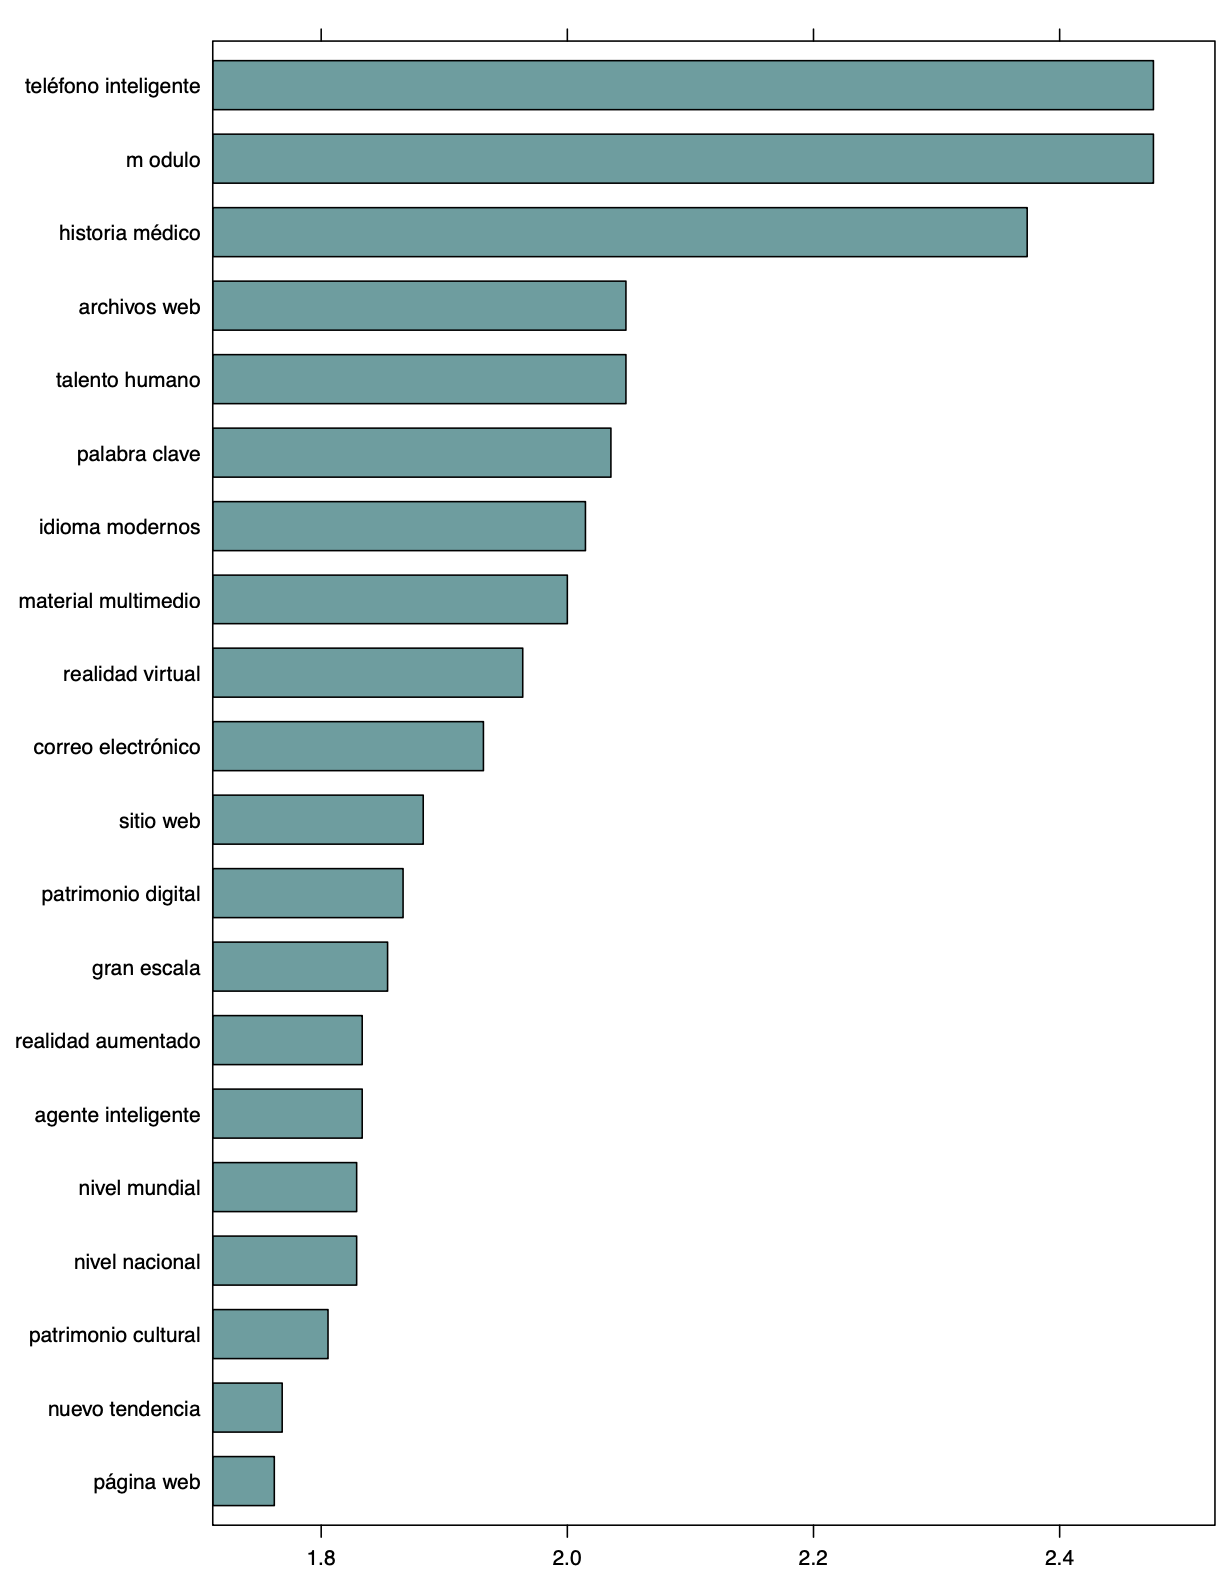
\includegraphics[width=0.6\linewidth]{images/05-desarrollo/2_ciclo/nlp/computacion_noun_adj} 

}

\caption{Palabras Claves en investigaciones de la Escuela de Computación}\label{fig:compususadj}
\end{figure}

La tabla que conforma el Corpus Anotado para esta fase de la Investigación se alojó en memoria RAM en una estructura de datos tabular denominada \emph{dataframe} del lenguaje R, sin ser registrada en un gestor de base de datos.

\hypertarget{aprender-3}{%
\paragraph{Aprender:}\label{aprender-3}}

Al analizar el Corpus anotado se detectaron algunos puntos a considerar para análisis posteriores.

\begin{itemize}
\item
  El proceso de separación por tokens y de lematización, como ya se mencionó, se hizo con la librería ``spacyr'', que hace estos procesos mediante el uso de un modelo preentrenado de aprendizaje automático. Hubo ciertas palabras, o términos que son muy específicos de un área de conocimiento, como en la química, donde los \emph{compuestos, moléculas, nomenclaturas} u otros, contienen denominaciones conformadas por cadenas de letras mayúsculas seguidas de puntos, que no presentan estructuras gramaticales propias del lenguaje natural, sino de un dominio específico, ver figura \ref{fig:quimica}. Al tener un modelo intentando hacer la separación de los tokens o el etiquetado, bajo unos textos con los cuales no fue entrenado, el proceso falla en la clasificación. Este problema, para ese tipo de términos, no fue resuelto al no disponer con un modelo entrenado para este dominio. En investigaciones posteriores pudiera realizarse un sobreentrenamiento que incluyera el etiquetado de estos \emph{tokens} de dominios muy especializados, como generalmente se presenta en carreras científicas y así poder mejorar la fase del etiquetado de las funciones gramaticales (POS).

  \begin{figure}

  {\centering 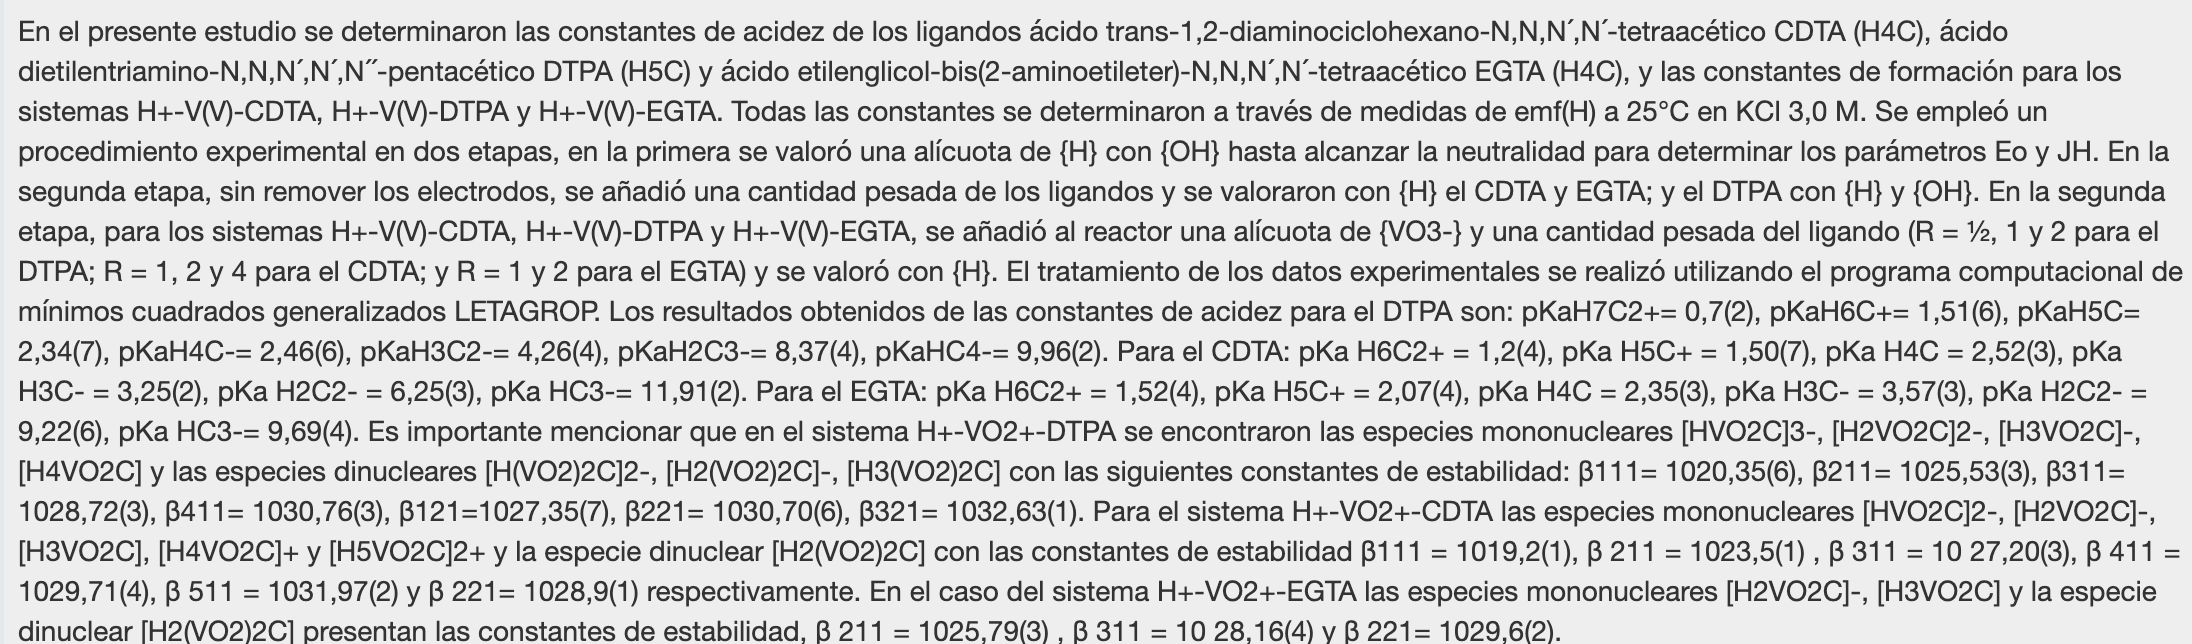
\includegraphics[width=0.85\linewidth]{images/05-desarrollo/2_ciclo/quimica} 

  }

  \caption{Texto "Resumen" de Trabajo de Grado de Maestría en Química. Autora: Margarita González}\label{fig:quimica}
  \end{figure}
\item
  La lematización permitió reducir en un 17,5 \% el vocabulario al pasar de 101.066 palabras a 83.402 lemas. Específicamente los lemas que se van a usar en fases posteriores del análisis, son los que están categorizados en el etiquetado del discurso como ``ADJ'' (adjetivos) que totalizan 277.394 289.283, equivalentes a un 8,8\% del total de palabras y los ``NOUMS'' (sustantivos) son 693.475 equivalentes al 22\% de las palabras presentes en el corpus. En el registro en base de datos se conservará completo el corpus anotado independientemente de la función gramatical con se etiquetasen.
\item
  Los textos del ``Resumen'' que se encuentran en la ficha de cada trabajo alojado en Saber UCV, en 396 casos, equivalentes al 4.3\% del total, contienen una porción de texto en idioma inglés referente al ``Abstract'', siendo óptimo aislar únicamente las partes que se encuentran en idioma español para que funcione correctamente el ``etiquetado de la parte del discurso''.
\end{itemize}

\hypertarget{imrecomendacion}{%
\subsubsection{Iteración - Recomendación Documentos:}\label{imrecomendacion}}

En esta iteración se revisó la creación de recomendaciones de investigaciones, basándose en la similitud que presente un documento con el resto de los documentos presentes en el Corpus.

\hypertarget{especulaciuxf3n-5}{%
\paragraph{Especulación:}\label{especulaciuxf3n-5}}

Se ha determinado que los investigadores no necesariamente realizan la búsqueda de documentos que le puedan ser de interés mediante un \emph{query} que contenga términos claves sino a partir de un documento que les resulta de interés quieren localizar otros que puedan compartir ciertos aspectos \citep{zhou2018}.

La similitud de un documento con otro se puede entender, en esta implementación, como aquellos que tienden a compartir palabras y dentro de una ``term document matrix'' generan vectores similares \citep{jurafsky2009}. Es por esto que se considera que los documentos que presenten mayor similitud, pueden resultar de interés para los investigadores, expandiendo así las posibilidades de inspección del Corpus.

\hypertarget{colaboraciuxf3n-5}{%
\paragraph{Colaboración:}\label{colaboraciuxf3n-5}}

Mediante la creación de una ``term document matrix'', vista en \ref{tdm}, usando el framework para análisis cuantitativo de textos ``quanteda'' \citep{quanteda}, la matriz obtenida refleja características esenciales de los documentos, en lo relativo a las palabras que lo conforman y su frecuencia.

En cada fila de la matriz se representa un documento, también equivalente a un vector. Midiendo la similitud \emph{coseno}, revisada en \ref{similitud}, con la función \texttt{textstat\_simil}, entre un determinado documento y el resto de los que conforman el corpus, es viable determinar cuáles son los más ``parecidos''.

Se realizó un proceso iterativo para calcular la similitud coseno entre documentos y se pudo apreciar que los resultados de similitud pueden resultar de interés en diversos casos, como el que se muestra en la figura \ref{fig:similitudreco}.

\begin{figure}

{\centering 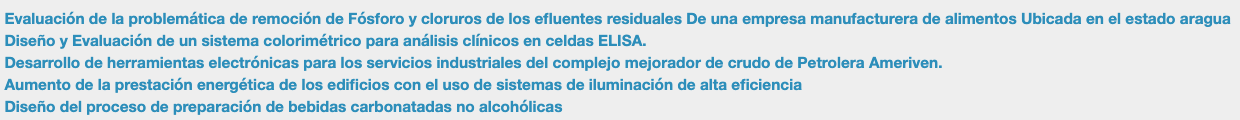
\includegraphics[width=0.9\linewidth]{images/05-desarrollo/2_ciclo/similitud_reco2} 

}

\caption{Resultado de recomendaciones al documento: "Diseño de un sistema para la desinfección de aguas de consumo humano y de uso industrial empleando un material inorgánico antibacterial"}\label{fig:similitudreco}
\end{figure}

\hypertarget{aprendizaje-1}{%
\paragraph{Aprendizaje:}\label{aprendizaje-1}}

Es necesario señalar que el método adaptado no es se considera que esté dentro del ``Estado del Arte'' para realizar recomendaciones, no obstante, se hace la evaluación de este recurso dentro del SCSU, al ser de sencilla implementación, cálculos rápidos, robustos que no consumen mayores recursos computacionales, los cuales quedan disponibles para otras tareas que ejecuta el SCSU.

\hypertarget{iterbol}{%
\subsubsection{Iteración- Implementación Prototipo:}\label{iterbol}}

En esta iteración se hace el desarrollo del Prototipo de un ``Sistema de Recuperación de Información'' que servirá de base para probar distintas funcionalidades con las cuales contará el Sistema Complementario Saber UCV. En particular se hace el Prototipo de la aplicación web, mediante el uso del framework Shiny \citep{shiny-2} y se establecen los casos de uso, para que el usuario pueda realizar procesos de búsqueda, sobre el corpus anotado que se conformó en la iteración anterior \ref{iternlp}.

En este Prototipo solo se va a trabajar con el subconjunto de las investigaciones que han sido realizadas en la Facultad de Ciencias y ante un \emph{query}, son extraídos los documentos que contengan tales palabras y con ellos se representan los ``Mapas de Conocimiento''.

Esta implementación se apoya en el uso del sistema gestor de base de datos PostgreSQL, ya que este software nativamente cuenta con la funcionalidad de construir un índice invertido, sobre un conjunto de documentos, y así se da sustento a las ``búsquedas de texto completo''.

\hypertarget{especulaciuxf3n-6}{%
\paragraph{Especulación:}\label{especulaciuxf3n-6}}

Contar con un prototipo permitirá evaluar las posibles interacciones entre el usuario y la versión que entre a producción del Sistema Complementario Saber UCV, así como analizar los tiempos de respuesta y los resultados de las visualizaciones.

Para el desarrollo de este prototipo se seleccionan los textos resúmenes que fueron categorizados como pertenecientes a la Facultad de Ciencias.

Durante la fase de especulación de este ciclo se realizaron los Diagramas de Caso de Uso que se ven en las figuras \ref{fig:protoUC1} y \ref{fig:protoUC11}:

\newpage

\begin{figure}

{\centering 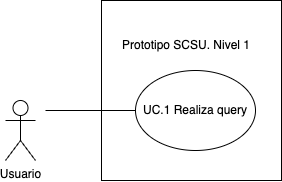
\includegraphics[width=0.45\linewidth]{images/05-desarrollo/2_ciclo/UC/prototipo_nivel1} 

}

\caption{Caso de Uso 1 - Prototipo SCSU - Nivel 1}\label{fig:protoUC1}
\end{figure}

\begin{figure}

{\centering 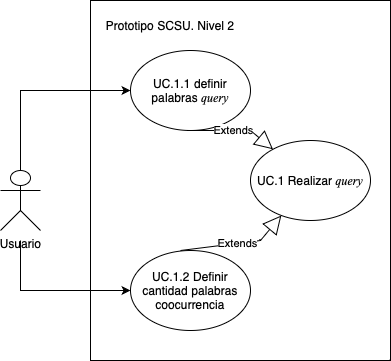
\includegraphics[width=0.45\linewidth]{images/05-desarrollo/2_ciclo/UC/prototipo_nivel2} 

}

\caption{Caso de Uso 1.1 - Prototipo SCSU - Nivel 2}\label{fig:protoUC11}
\end{figure}

En el cuadro \ref{tab:prototipoUC1} se muestra el caso de uso UC.1 del Prototipo del SCSU.

\newpage

\global\setlength{\Oldarrayrulewidth}{\arrayrulewidth}

\global\setlength{\Oldtabcolsep}{\tabcolsep}

\setlength{\tabcolsep}{0pt}

\renewcommand*{\arraystretch}{1.5}



\providecommand{\ascline}[3]{\noalign{\global\arrayrulewidth #1}\arrayrulecolor[HTML]{#2}\cline{#3}}

\begin{longtable}[c]{|p{1.00in}|p{6.00in}}

\caption{Prototipo\ SCSU\ UC.1}\label{tab:prototipoUC1}\\

\hhline{>{\arrayrulecolor[HTML]{666666}\global\arrayrulewidth=0.75pt}->{\arrayrulecolor[HTML]{666666}\global\arrayrulewidth=0.75pt}-}

\multicolumn{1}{!{\color[HTML]{666666}\vrule width 0.75pt}>{\cellcolor[HTML]{C2C2C2}\raggedright}m{\dimexpr 1in+0\tabcolsep}}{\textcolor[HTML]{000000}{\fontsize{10}{10}\selectfont{\global\setmainfont{Helvetica}{Nombre}}}} & \multicolumn{1}{!{\color[HTML]{666666}\vrule width 0.75pt}>{\raggedright}m{\dimexpr 6in+0\tabcolsep}!{\color[HTML]{666666}\vrule width 0.75pt}}{\textcolor[HTML]{000000}{\fontsize{10}{10}\selectfont{\global\setmainfont{Helvetica}{UC.1:\ Realizar\ proceso\ de\ recuperación\ de\ información\ (query)}}}} \\

\noalign{\global\arrayrulewidth 0.75pt}\arrayrulecolor[HTML]{666666}

\hhline{|>{\arrayrulecolor[HTML]{666666}\global\arrayrulewidth=0.75pt}-|>{\arrayrulecolor[HTML]{666666}\global\arrayrulewidth=0.75pt}-}



\multicolumn{1}{!{\color[HTML]{666666}\vrule width 0.75pt}>{\cellcolor[HTML]{C2C2C2}\raggedright}m{\dimexpr 1in+0\tabcolsep}}{\textcolor[HTML]{000000}{\fontsize{10}{10}\selectfont{\global\setmainfont{Helvetica}{Descripción}}}} & \multicolumn{1}{!{\color[HTML]{666666}\vrule width 0.75pt}>{\raggedright}m{\dimexpr 6in+0\tabcolsep}!{\color[HTML]{666666}\vrule width 0.75pt}}{\textcolor[HTML]{000000}{\fontsize{10}{10}\selectfont{\global\setmainfont{Helvetica}{El\ usuario\ realiza\ búsquedas\ sobre\ los\ textos\ que\ conforman\ el\ Corpus\ del\ Prototipo}}}} \\

\noalign{\global\arrayrulewidth 0.75pt}\arrayrulecolor[HTML]{666666}

\hhline{|>{\arrayrulecolor[HTML]{666666}\global\arrayrulewidth=0.75pt}-|>{\arrayrulecolor[HTML]{666666}\global\arrayrulewidth=0.75pt}-}



\multicolumn{1}{!{\color[HTML]{666666}\vrule width 0.75pt}>{\cellcolor[HTML]{C2C2C2}\raggedright}m{\dimexpr 1in+0\tabcolsep}}{\textcolor[HTML]{000000}{\fontsize{10}{10}\selectfont{\global\setmainfont{Helvetica}{Actor}}}} & \multicolumn{1}{!{\color[HTML]{666666}\vrule width 0.75pt}>{\raggedright}m{\dimexpr 6in+0\tabcolsep}!{\color[HTML]{666666}\vrule width 0.75pt}}{\textcolor[HTML]{000000}{\fontsize{10}{10}\selectfont{\global\setmainfont{Helvetica}{usuario}}}} \\

\noalign{\global\arrayrulewidth 0.75pt}\arrayrulecolor[HTML]{666666}

\hhline{|>{\arrayrulecolor[HTML]{666666}\global\arrayrulewidth=0.75pt}-|>{\arrayrulecolor[HTML]{666666}\global\arrayrulewidth=0.75pt}-}



\multicolumn{2}{!{\color[HTML]{666666}\vrule width 0.75pt}>{\cellcolor[HTML]{8F8F8F}\centering}m{\dimexpr 7in+2\tabcolsep+0.75pt}!{\color[HTML]{666666}\vrule width 0.75pt}}{\textcolor[HTML]{000000}{\fontsize{10}{10}\selectfont{\global\setmainfont{Helvetica}{Flujo\ de\ Eventos}}}} \\

\noalign{\global\arrayrulewidth 0.75pt}\arrayrulecolor[HTML]{666666}

\hhline{|>{\arrayrulecolor[HTML]{666666}\global\arrayrulewidth=0.75pt}-|>{\arrayrulecolor[HTML]{666666}\global\arrayrulewidth=0.75pt}-}



\multicolumn{2}{!{\color[HTML]{666666}\vrule width 0.75pt}>{\cellcolor[HTML]{A3A3A3}\raggedright}m{\dimexpr 7in+2\tabcolsep+0.75pt}!{\color[HTML]{666666}\vrule width 0.75pt}}{\textcolor[HTML]{000000}{\fontsize{10}{10}\selectfont{\global\setmainfont{Helvetica}{Flujo\ Básico}}}} \\

\noalign{\global\arrayrulewidth 0.75pt}\arrayrulecolor[HTML]{666666}

\hhline{|>{\arrayrulecolor[HTML]{666666}\global\arrayrulewidth=0.75pt}-|>{\arrayrulecolor[HTML]{666666}\global\arrayrulewidth=0.75pt}-}



\multicolumn{2}{!{\color[HTML]{666666}\vrule width 0.75pt}>{\raggedright}m{\dimexpr 7in+2\tabcolsep+0.75pt}!{\color[HTML]{666666}\vrule width 0.75pt}}{\textcolor[HTML]{000000}{\fontsize{10}{10}\selectfont{\global\setmainfont{Helvetica}{El\ caso\ de\ uso\ inicia\ cuando\ el\ usuario\ ingresa\ a\ la\ aplicación\ y\ el\ prototipo\ muesta\ dos\ campos:\ }}}\textcolor[HTML]{000000}{\fontsize{10}{10}\selectfont{\global\setmainfont{Helvetica}{\linebreak }}}\textcolor[HTML]{000000}{\fontsize{10}{10}\selectfont{\global\setmainfont{Helvetica}{\ 1)\ En\ el\ primero\ debe\ introducir\ el\ texto\ a\ buscar.\ }}}\textcolor[HTML]{000000}{\fontsize{10}{10}\selectfont{\global\setmainfont{Helvetica}{\linebreak }}}\textcolor[HTML]{000000}{\fontsize{10}{10}\selectfont{\global\setmainfont{Helvetica}{\ 2)\ En\ el\ segundo,\ en\ el\ que\ aparece\ por\ defecto\ el\ valor\ 60,\ se\ corresponde\ con\ las\ cantidades\ de\ coocurrencias\ que\ serán\ presentadas\ en\ los\ "Mapas\ del\ Conocimiento".\ }}}\textcolor[HTML]{000000}{\fontsize{10}{10}\selectfont{\global\setmainfont{Helvetica}{\linebreak }}}\textcolor[HTML]{000000}{\fontsize{10}{10}\selectfont{\global\setmainfont{Helvetica}{\ 3)\ El\ usuario\ hace\ "clic"\ en\ el\ "buscar\ palabras"\ }}}\textcolor[HTML]{000000}{\fontsize{10}{10}\selectfont{\global\setmainfont{Helvetica}{\linebreak }}}\textcolor[HTML]{000000}{\fontsize{10}{10}\selectfont{\global\setmainfont{Helvetica}{\ 4)\ El\ Prototipo\ presenta\ los\ resultados\ obtenidos\ }}}\textcolor[HTML]{000000}{\fontsize{10}{10}\selectfont{\global\setmainfont{Helvetica}{\linebreak }}}\textcolor[HTML]{000000}{\fontsize{10}{10}\selectfont{\global\setmainfont{Helvetica}{\ 5)\ El\ caso\ de\ uso\ termina}}}} \\

\noalign{\global\arrayrulewidth 0.75pt}\arrayrulecolor[HTML]{666666}

\hhline{|>{\arrayrulecolor[HTML]{666666}\global\arrayrulewidth=0.75pt}-|>{\arrayrulecolor[HTML]{666666}\global\arrayrulewidth=0.75pt}-}



\multicolumn{2}{!{\color[HTML]{666666}\vrule width 0.75pt}>{\cellcolor[HTML]{A3A3A3}\raggedright}m{\dimexpr 7in+2\tabcolsep+0.75pt}!{\color[HTML]{666666}\vrule width 0.75pt}}{\textcolor[HTML]{000000}{\fontsize{10}{10}\selectfont{\global\setmainfont{Helvetica}{Flujo\ Alternativo}}}} \\

\noalign{\global\arrayrulewidth 0.75pt}\arrayrulecolor[HTML]{666666}

\hhline{|>{\arrayrulecolor[HTML]{666666}\global\arrayrulewidth=0.75pt}-|>{\arrayrulecolor[HTML]{666666}\global\arrayrulewidth=0.75pt}-}



\multicolumn{1}{!{\color[HTML]{666666}\vrule width 0.75pt}>{\cellcolor[HTML]{C2C2C2}\raggedright}m{\dimexpr 1in+0\tabcolsep}}{\textcolor[HTML]{000000}{\fontsize{10}{10}\selectfont{\global\setmainfont{Helvetica}{Título}}}} & \multicolumn{1}{!{\color[HTML]{666666}\vrule width 0.75pt}>{\cellcolor[HTML]{C2C2C2}\raggedright}m{\dimexpr 6in+0\tabcolsep}!{\color[HTML]{666666}\vrule width 0.75pt}}{\textcolor[HTML]{000000}{\fontsize{10}{10}\selectfont{\global\setmainfont{Helvetica}{Descripción}}}} \\

\noalign{\global\arrayrulewidth 0.75pt}\arrayrulecolor[HTML]{666666}

\hhline{|>{\arrayrulecolor[HTML]{666666}\global\arrayrulewidth=0.75pt}-|>{\arrayrulecolor[HTML]{666666}\global\arrayrulewidth=0.75pt}-}



\multicolumn{1}{!{\color[HTML]{666666}\vrule width 0.75pt}>{\raggedright}m{\dimexpr 1in+0\tabcolsep}}{\textcolor[HTML]{000000}{\fontsize{10}{10}\selectfont{\global\setmainfont{Helvetica}{N/A}}}} & \multicolumn{1}{!{\color[HTML]{666666}\vrule width 0.75pt}>{\raggedright}m{\dimexpr 6in+0\tabcolsep}!{\color[HTML]{666666}\vrule width 0.75pt}}{\textcolor[HTML]{000000}{\fontsize{10}{10}\selectfont{\global\setmainfont{Helvetica}{N/A}}}} \\

\noalign{\global\arrayrulewidth 0.75pt}\arrayrulecolor[HTML]{666666}

\hhline{|>{\arrayrulecolor[HTML]{666666}\global\arrayrulewidth=0.75pt}-|>{\arrayrulecolor[HTML]{666666}\global\arrayrulewidth=0.75pt}-}



\multicolumn{2}{!{\color[HTML]{666666}\vrule width 0.75pt}>{\cellcolor[HTML]{A3A3A3}\centering}m{\dimexpr 7in+2\tabcolsep+0.75pt}!{\color[HTML]{666666}\vrule width 0.75pt}}{\textcolor[HTML]{000000}{\fontsize{10}{10}\selectfont{\global\setmainfont{Helvetica}{Precondiciones}}}} \\

\noalign{\global\arrayrulewidth 0.75pt}\arrayrulecolor[HTML]{666666}

\hhline{|>{\arrayrulecolor[HTML]{666666}\global\arrayrulewidth=0.75pt}-|>{\arrayrulecolor[HTML]{666666}\global\arrayrulewidth=0.75pt}-}



\multicolumn{1}{!{\color[HTML]{666666}\vrule width 0.75pt}>{\cellcolor[HTML]{C2C2C2}\raggedright}m{\dimexpr 1in+0\tabcolsep}}{\textcolor[HTML]{000000}{\fontsize{10}{10}\selectfont{\global\setmainfont{Helvetica}{Título}}}} & \multicolumn{1}{!{\color[HTML]{666666}\vrule width 0.75pt}>{\cellcolor[HTML]{C2C2C2}\raggedright}m{\dimexpr 6in+0\tabcolsep}!{\color[HTML]{666666}\vrule width 0.75pt}}{\textcolor[HTML]{000000}{\fontsize{10}{10}\selectfont{\global\setmainfont{Helvetica}{Descripción}}}} \\

\noalign{\global\arrayrulewidth 0.75pt}\arrayrulecolor[HTML]{666666}

\hhline{|>{\arrayrulecolor[HTML]{666666}\global\arrayrulewidth=0.75pt}-|>{\arrayrulecolor[HTML]{666666}\global\arrayrulewidth=0.75pt}-}



\multicolumn{1}{!{\color[HTML]{666666}\vrule width 0.75pt}>{\raggedright}m{\dimexpr 1in+0\tabcolsep}}{\textcolor[HTML]{000000}{\fontsize{10}{10}\selectfont{\global\setmainfont{Helvetica}{N/A}}}} & \multicolumn{1}{!{\color[HTML]{666666}\vrule width 0.75pt}>{\raggedright}m{\dimexpr 6in+0\tabcolsep}!{\color[HTML]{666666}\vrule width 0.75pt}}{\textcolor[HTML]{000000}{\fontsize{10}{10}\selectfont{\global\setmainfont{Helvetica}{N/A}}}} \\

\noalign{\global\arrayrulewidth 0.75pt}\arrayrulecolor[HTML]{666666}

\hhline{|>{\arrayrulecolor[HTML]{666666}\global\arrayrulewidth=0.75pt}-|>{\arrayrulecolor[HTML]{666666}\global\arrayrulewidth=0.75pt}-}



\multicolumn{2}{!{\color[HTML]{666666}\vrule width 0.75pt}>{\cellcolor[HTML]{A3A3A3}\centering}m{\dimexpr 7in+2\tabcolsep+0.75pt}!{\color[HTML]{666666}\vrule width 0.75pt}}{\textcolor[HTML]{000000}{\fontsize{10}{10}\selectfont{\global\setmainfont{Helvetica}{Postcondiciones}}}} \\

\noalign{\global\arrayrulewidth 0.75pt}\arrayrulecolor[HTML]{666666}

\hhline{|>{\arrayrulecolor[HTML]{666666}\global\arrayrulewidth=0.75pt}-|>{\arrayrulecolor[HTML]{666666}\global\arrayrulewidth=0.75pt}-}



\multicolumn{1}{!{\color[HTML]{666666}\vrule width 0.75pt}>{\cellcolor[HTML]{C2C2C2}\raggedright}m{\dimexpr 1in+0\tabcolsep}}{\textcolor[HTML]{000000}{\fontsize{10}{10}\selectfont{\global\setmainfont{Helvetica}{Título}}}} & \multicolumn{1}{!{\color[HTML]{666666}\vrule width 0.75pt}>{\cellcolor[HTML]{C2C2C2}\raggedright}m{\dimexpr 6in+0\tabcolsep}!{\color[HTML]{666666}\vrule width 0.75pt}}{\textcolor[HTML]{000000}{\fontsize{10}{10}\selectfont{\global\setmainfont{Helvetica}{Descripción}}}} \\

\noalign{\global\arrayrulewidth 0.75pt}\arrayrulecolor[HTML]{666666}

\hhline{|>{\arrayrulecolor[HTML]{666666}\global\arrayrulewidth=0.75pt}-|>{\arrayrulecolor[HTML]{666666}\global\arrayrulewidth=0.75pt}-}



\multicolumn{1}{!{\color[HTML]{666666}\vrule width 0.75pt}>{\raggedright}m{\dimexpr 1in+0\tabcolsep}}{\textcolor[HTML]{000000}{\fontsize{10}{10}\selectfont{\global\setmainfont{Helvetica}{Éxito}}}} & \multicolumn{1}{!{\color[HTML]{666666}\vrule width 0.75pt}>{\raggedright}m{\dimexpr 6in+0\tabcolsep}!{\color[HTML]{666666}\vrule width 0.75pt}}{\textcolor[HTML]{000000}{\fontsize{10}{10}\selectfont{\global\setmainfont{Helvetica}{El\ prototipo\ presenta:\ }}}\textcolor[HTML]{000000}{\fontsize{10}{10}\selectfont{\global\setmainfont{Helvetica}{\linebreak }}}\textcolor[HTML]{000000}{\fontsize{10}{10}\selectfont{\global\setmainfont{Helvetica}{\ 1)\ Total\ de\ investigaciones\ por\ jeraraquías\ de\ las\ investigaciones\ que\ fueron\ recuperadas\ }}}\textcolor[HTML]{000000}{\fontsize{10}{10}\selectfont{\global\setmainfont{Helvetica}{\linebreak }}}\textcolor[HTML]{000000}{\fontsize{10}{10}\selectfont{\global\setmainfont{Helvetica}{\ 2)\ Gráfico\ con\ "Mapas\ de\ Conocimiento".\ }}}\textcolor[HTML]{000000}{\fontsize{10}{10}\selectfont{\global\setmainfont{Helvetica}{\linebreak }}}\textcolor[HTML]{000000}{\fontsize{10}{10}\selectfont{\global\setmainfont{Helvetica}{\ 3)\ Tabla\ con\ datos\ de\ los\ texto\ Resumen\ recuperados\ de\ acuerdo\ al\ query}}}} \\

\noalign{\global\arrayrulewidth 0.75pt}\arrayrulecolor[HTML]{666666}

\hhline{|>{\arrayrulecolor[HTML]{666666}\global\arrayrulewidth=0.75pt}-|>{\arrayrulecolor[HTML]{666666}\global\arrayrulewidth=0.75pt}-}



\multicolumn{1}{!{\color[HTML]{666666}\vrule width 0.75pt}>{\raggedright}m{\dimexpr 1in+0\tabcolsep}}{\textcolor[HTML]{000000}{\fontsize{10}{10}\selectfont{\global\setmainfont{Helvetica}{Fracaso}}}} & \multicolumn{1}{!{\color[HTML]{666666}\vrule width 0.75pt}>{\raggedright}m{\dimexpr 6in+0\tabcolsep}!{\color[HTML]{666666}\vrule width 0.75pt}}{\textcolor[HTML]{000000}{\fontsize{10}{10}\selectfont{\global\setmainfont{Helvetica}{N/A}}}} \\

\noalign{\global\arrayrulewidth 0.75pt}\arrayrulecolor[HTML]{666666}

\hhline{|>{\arrayrulecolor[HTML]{666666}\global\arrayrulewidth=0.75pt}-|>{\arrayrulecolor[HTML]{666666}\global\arrayrulewidth=0.75pt}-}



\end{longtable}



\arrayrulecolor[HTML]{000000}

\global\setlength{\arrayrulewidth}{\Oldarrayrulewidth}

\global\setlength{\tabcolsep}{\Oldtabcolsep}

\renewcommand*{\arraystretch}{1}

En la figura \ref{fig:sidebar} se muestra el mock-up de la Interfaz para el prototipo del SCSU.

\begin{figure}

{\centering 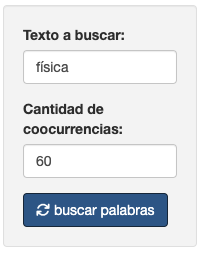
\includegraphics[width=0.25\linewidth]{images/05-desarrollo/2_ciclo/UI/prototipo_sidebar} 

}

\caption{Mock-Up de campos de entrada en la Interfaz del Prototipo}\label{fig:sidebar}
\end{figure}

En cuanto a los ``Mapas de Conocimiento (MC)'', motivado a que visualizar gráficamente los resultados es una forma conveniente de ayudar a los usuarios a descubrir relaciones y patrones presentes en los textos que pueden estar ocultos \citep{li2018}, en la figura \ref{fig:mapacon} se muestra la propuesta de representación de los ``MC'' en el Prototipo.

\begin{figure}

{\centering 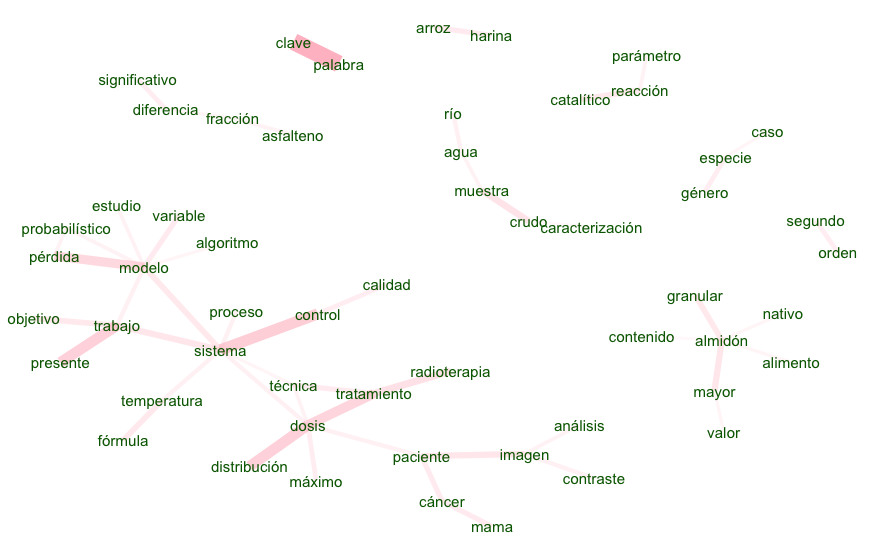
\includegraphics[width=0.7\linewidth]{images/05-desarrollo/2_ciclo/UI/mapcon} 

}

\caption{Representación Mapas de Conocimiento}\label{fig:mapacon}
\end{figure}

Para poder implementar la búsqueda de texto se usará \emph{postgreSQL V16}, por lo cual en la fase de ``especulación'' se realizó el diseño del modelo ``entidad-relación'' que se ve en detalle en la figura \ref{fig:entrel}.

\begin{figure}

{\centering 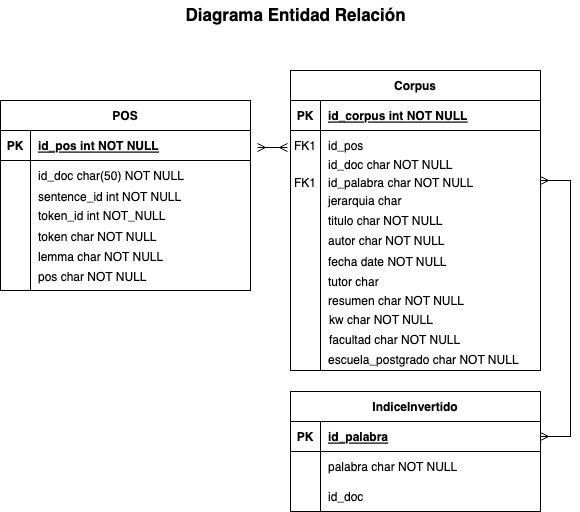
\includegraphics[width=0.6\linewidth]{images/05-desarrollo/2_ciclo/esquemas/diagrama_entidadrel} 

}

\caption{Modelo Entidad-Relación}\label{fig:entrel}
\end{figure}

En el modelo, la entidad ``Corpus'' se apoya en la tabla ``POS'' que contiene el detalle del etiquetado de la parte del discurso para cada palabra (token) presente en cada documento, mientras que la tabla ``Indice Invertido'' se destinará a almacenar la estructura que permite general la búsqueda de texto y básicamente almacena cada palabra que compone el vocabulario y el \emph{id} de los documentos donde aparece cada palabra.

Un factor determinante para la selección de PostgreSQL es el soporte que tiene para ejecutar procesos de ``Busqueda de Texto Completo (\emph{Full Text Search})'' en el idioma español.

El esquema de la arquitectura general de la aplicación, el cuál se implementará en el \emph{framework} shiny, se representa en la figura \ref{fig:esqshinyproto}.

\begin{figure}

{\centering 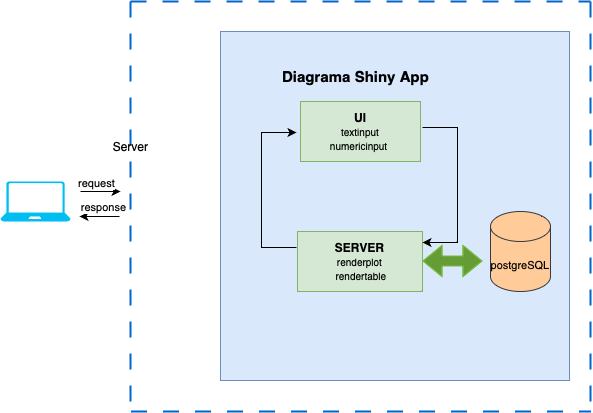
\includegraphics[width=0.5\linewidth]{images/05-desarrollo/2_ciclo/esquemas/shinyappproto} 

}

\caption{Esquema General del Prototipo de la Aplicación}\label{fig:esqshinyproto}
\end{figure}

\hypertarget{colaboraciuxf3n-6}{%
\paragraph{Colaboración:}\label{colaboraciuxf3n-6}}

La aplicación web que formará parte del Prototipo, una vez que se tiene conformado el corpus anotado, como se vio en \ref{iternlp}, se debe iniciar el ``Poblado de la Base de Dato'' con las tres tablas que se mostraron en el diagrama de entidad relación propuesto en \ref{fig:entrel} . A continuación se van a describir los procesos con los que se realizó el ``Poblado\textbf{``} que sirve al Prototipo.

\begin{enumerate}
\def\labelenumi{\arabic{enumi}.}
\item
  \textbf{Tabla Corpus}: con los datos del Corpus Anotado, se conforma la tabla con los siguientes datos: jerarquía, título, nombre autor, fecha publicación, nombre de tutor, texto resumen, palabras claves, nombre de la facultad y nombre de la escuela-postgrado y el código único identificador de cada documento.
\item
  \textbf{Tabla ``indiceinvertido'':} mediante una extensión de \emph{PostrgreSQL V16.1} denominada \texttt{"TS\_Vector}``, se crea una columna de nombre \texttt{"document\_tokens"}, donde se almacena una estructura de datos de tipo''\texttt{tsvector}``, que facilita al gestor de BD la búsqueda de texto completo. El script siguiente hace el trabajo de crear el índice invertido mediante la función \texttt{"to\_tsvector"}, para los datos del''título'', ``palabras claves'', ``autor'' y del ``resumen''. En el mismo proceso se añaden pesos distintos (importancia para el criterio de reordenamiento de los resultados, según lo revisado en \ref{ranking} ) a cada atributo mediante la función \texttt{"setweight"}.

  \newpage

\begin{Shaded}
\begin{Highlighting}[]
\KeywordTok{ALTER} \KeywordTok{TABLE}\NormalTok{ Corpus }\KeywordTok{ADD} \KeywordTok{COLUMN}\NormalTok{ document\_tokens tsvector}
\KeywordTok{GENERATED}\NormalTok{ ALWAYS }\KeywordTok{AS}\NormalTok{ ((setweight(to\_tsvector(}\StringTok{\textquotesingle{}spanish\textquotesingle{}}\NormalTok{,}
                        \FunctionTok{coalesce}\NormalTok{(autor,}\StringTok{\textquotesingle{}\textquotesingle{}}\NormalTok{)),}\StringTok{\textquotesingle{}A\textquotesingle{}}\NormalTok{) }\OperatorTok{||}  
\NormalTok{                      setweight(to\_tsvector(}\StringTok{\textquotesingle{}spanish\textquotesingle{}}\NormalTok{,}
                        \FunctionTok{coalesce}\NormalTok{(titulo,}\StringTok{\textquotesingle{}\textquotesingle{}}\NormalTok{)),}\StringTok{\textquotesingle{}B\textquotesingle{}}\NormalTok{)}\OperatorTok{||}  
\NormalTok{                      setweight(to\_tsvector(}\StringTok{\textquotesingle{}spanish\textquotesingle{}}\NormalTok{,}
                        \FunctionTok{coalesce}\NormalTok{(kw,}\StringTok{\textquotesingle{}\textquotesingle{}}\NormalTok{)),}\StringTok{\textquotesingle{}C\textquotesingle{}}\NormalTok{)    }\OperatorTok{||}  
\NormalTok{                        setweight(to\_tsvector(}\StringTok{\textquotesingle{}spanish\textquotesingle{}}\NormalTok{,}
                        \FunctionTok{coalesce}\NormalTok{(resumen,}\StringTok{\textquotesingle{}\textquotesingle{}}\NormalTok{)),}\StringTok{\textquotesingle{}D\textquotesingle{}}\NormalTok{))) STORED;}
\end{Highlighting}
\end{Shaded}

  En la figura \ref{fig:doctok} se puede ver parcialmente la estructura de datos de tipo ``\texttt{tsvector}'' que se genera para el texto ``Las planicies de inundación son sistemas asociados al margen de un río que están sujetas a pulsos estacionales de inundación y sequía. La desembocadura del Río Mapire constituye un sistema complejo de planicie de inundación, como resultado del aumento del nivel de agua en el río por un efecto de represamiento por el Río Orinoco durante la época lluviosa. El gradiente de inundación que se forma genera un estrés ambiental en el sistema suelo que depende de la duración y profundidad\ldots.'' .

  \begin{figure}

  {\centering 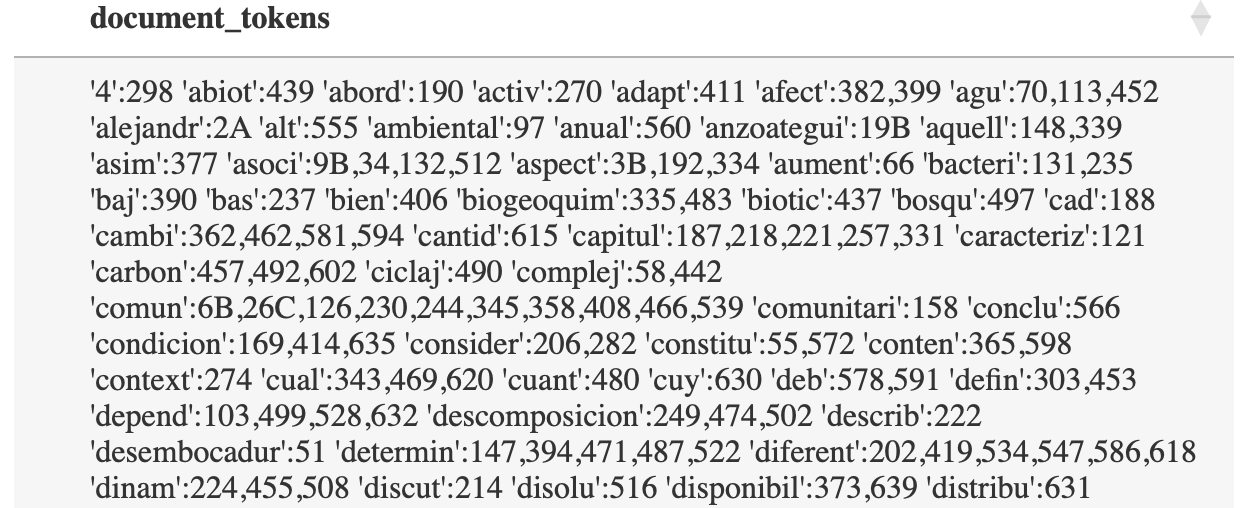
\includegraphics[width=0.7\linewidth]{images/05-desarrollo/2_ciclo/esquemas/doc_tokens} 

  }

  \caption{Estructura de datos Índice Invertido}\label{fig:doctok}
  \end{figure}

  La función \texttt{"to\_tsvector"} hace el parseo de un documento a tokens y estos son modificados realizando el \emph{stemming} para extraer la raíz de la palabra, proceso que se revisó en \ref{steaming}, lo cual ayuda a disminuir el espacio de búsqueda y a realizar las recuperación de textos de manera más eficiente. Para lograr ejecutar este proceso, es necesario dar el parámetro ``spanish'' a la función, para que sea sobre la base del idioma español, que sea extraída la raíz.

  La posición de la palabra dentro del texto, también queda registrada para así poder determinar en un \emph{query} de varias palabras, la cercanía que tienen dentro del texto las palabras que son buscadas, dando una mayor relevancia a las que estén más cercanas.

  Otro aspecto a destacar es que ciertas palabras de uso común y frecuente, denominadas \emph{stopwords}, como: ``el'', ``la'', ``y'', ``a'', ``en'', ``con'', ``para''; no son registradas, es decir que son omitidas así como los signos de puntuación, con lo cual un query que contenga una stopword o un signo de puntuación, no será buscada la coincidencia al no formar parte de la estructura de datos ``\texttt{tsvector}''.

  Para culminar el proceso de creación del ``Índice Invertido'' se debe ejecutar el comando \texttt{"CREATE\ INDEX\ document\_weights\_idx\ ON\ Corpus\ USING\ GIN\ (document\_tokens);"} que cierra el ciclo de la generación del índice y es lo que permite realizar los procesos de búsqueda en una forma más eficiente, disminuyendo los tiempos de respuesta, pero debiendo tener presente que la creación del índice puede incrementar entre un cincuenta y doscientos por ciento el espacio de almacenamiento al generarlo. Una de las bondades que adicionalmente brinda la función \texttt{"TS\_VECTOR"},es que al añadir nuevos documentos a la base de datos, el índice será actualizado automáticamente.
\item
  \textbf{Tabla ``POS'':} con los procesos que fueron revisados en el etiquetado de la parte del discurso en \ref{iternlp}, se obtuvieron los datos que formarán parte de esta tabla, donde cada palabra que conforma el corpus, pasa a ser una fila identificando el documento de origen, la oración dentro del documento donde se encuentra la palabra, el número de orden de aparición de la palabra, la palabra, su lema y la función gramatical asignada, idéntico a lo que se observó en la figura \ref{fig:spacypi}.
\end{enumerate}

En cuanto a la aplicación web, mediante el \emph{framework} Shiny se implementó el Prototipo, con la codificación de dos componentes principales que son: la interfaz de usuario (UI) y el Servidor (Server).

Shiny se basa en la ``programación reactiva'', lo que significa que ante cambios en los ``campos de entrada'' en la interfaz de usario (UI), los elementos asociados se actualizan dinámicamente desde el componente ``Server'' sin necesidad de recargar la página, permitiendo crear una experiencia al usuario fluida. Shiny utiliza conceptos como ``observadores'' y ``reactividad'' para mantener sincronizados los elementos de la UI con los datos subyacentes, que en el caso del Prototipo son el texto del \emph{query}, el valor para establecer la cantidad de coocurrencias a representar en el Mapa del Conocimiento y el botón para ejecutar el \emph{query}.

\hfill\break
A nivel de la aplicación web, en la interfaz de usuario están estos tres componentes:

\begin{enumerate}
\def\labelenumi{\arabic{enumi}.}
\item
  \textbf{textInput}: que corresponde a la casilla del \emph{query}.
\item
  \textbf{numericInput}: la cantidad de palabras que se van a mostrar en la representación de los Mapas de Conocimiento.
\item
  \textbf{actionBttn}: botón de acción para ejecutar el query.
\end{enumerate}

En el servidor de la aplicación, a nivel de generación de estructuras a ser representadas como resultados, dispone de estos componentes:

\begin{enumerate}
\def\labelenumi{\arabic{enumi}.}
\item
  \textbf{dataTableOutput}: mediante la librería ``datatable'' \citep{DT} se genera una tabla con los resultados obtenidos donde se incluyen los atributos: ``Fecha'',``Títutlo'', ``Autor'', ``Resumen'', ``Facultad'', ``Escuela'', ``Nombre Tutor''.
\item
  \textbf{renderPlot}: con el uso de la librería ``ggraph'' \citep{ggraph} se crea un grafo que reproduce los ``Mapas de Conocimiento'', representando las palabras mediante nodos y la coocurrencia implica la unión mediante arcos, y a mayor grosor en el arco, quiere decir que la cantidad de veces que se presenta la coocurrencia es mayor.
\end{enumerate}

En la figura \ref{fig:prototipoapp} se muestra la versión implementada del prototipo donde ante la búsqueda de la palabra ``física'', se recuperan los documentos que incluyen tal palabra y se generan los ``Mapas de Conocimiento''.

\begin{figure}

{\centering 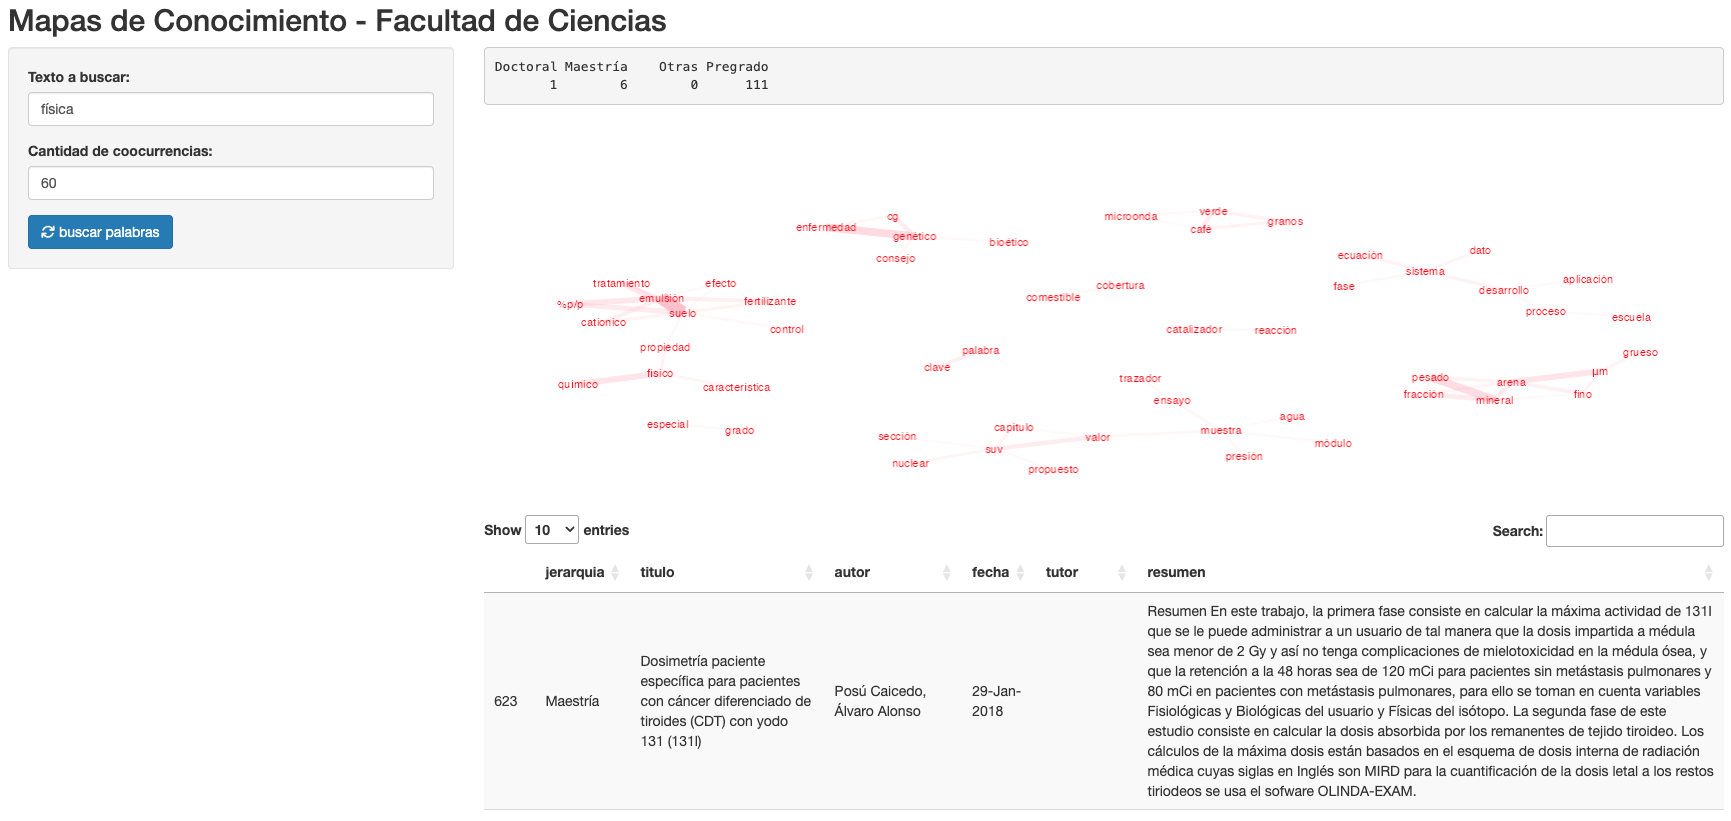
\includegraphics[width=0.8\linewidth]{images/05-desarrollo/2_ciclo/UI/prototipo_app} 

}

\caption{Estructura de datos Índice Invertido}\label{fig:prototipoapp}
\end{figure}

Explicación de los servicios ofrecidos por la aplicación: el usuario introduce un texto con el cual se va a generar el query y la cantidad de palabras que quiere visualizar en los Mapas de Conocimiento. Posteriormente hace clic en ``buscar palabras''.

\textbf{Lógica de la aplicación:}

En el detalle que se expone en las siguientes líneas es necesario mencionar que Shiny, funciona a nivel de computo como monohilo (``single-threaded''), por lo cual es estrictamente necesario que los pasos sean ejecutados secuencialmente según lo descrito.

\begin{enumerate}
\def\labelenumi{\arabic{enumi}.}
\item
  \textbf{Definición ``texto búsqueda'':} el usuario define el texto del query y la cantidad de coocurrencias.
\item
  \textbf{Procesamiento Query texto:} Cuando el servidor recibe el texto para generar el \emph{query}, este es procesado con la sintaxis del siguiente código:

\begin{Shaded}
\begin{Highlighting}[]
\OtherTok{"select titulo, id\_doc, facultad, jerarquia ,fecha,}
\NormalTok{  autor, kw, resumen, nombre, tutor }\KeywordTok{from}\NormalTok{ Corpus }\KeywordTok{where}
\NormalTok{  document\_tokens @@ websearch\_to\_tsquery(}\StringTok{\textquotesingle{}spanish\textquotesingle{}}\NormalTok{,}
    \StringTok{\textquotesingle{}texto a buscar\textquotesingle{}}\NormalTok{) }
  \KeywordTok{order} \KeywordTok{by}\NormalTok{ ts\_rank\_cd (document\_tokens,}
\NormalTok{    websearch\_to\_tsquery(}\StringTok{\textquotesingle{}spanish\textquotesingle{}}\NormalTok{,}\StringTok{\textquotesingle{}texto a buscar\textquotesingle{}}\NormalTok{)) }\KeywordTok{desc}
\end{Highlighting}
\end{Shaded}

  Lo relevante, es apreciar que el texto del \emph{query}, mediante la función \texttt{"websearch\_to\_tsquery"}, es sometido a un parseo que lo convierte a la estructura de datos ``\texttt{tsvector"} que fue revisada anteriormente y así la hace compatible con el contenido de la columna''\texttt{document\_tokens"} . El operador de coincidencia ``\texttt{@@}'' es el que determina si el texto del \texttt{tsquery} coincide con los distintos textos registrados en el ``\texttt{tsvector"} . Si la frase del query, por ejemplo''física química'', que incluye dos palabras, el operador lógico que se intercala entre cada palabra es el ``y (and)'', no obstante, la propia función \texttt{websearch\_to\_tsquery} permite que se defina que pueda ser el operador ``o (or)'', por ejemplo si se escribe ``física OR química''. \footnote{Otros operadores que se pueden usar en esta función son: ``!'' para excluir un término, ``\textless-\textgreater{}'' para indicar que las palabras deben aparecer una seguida de otra. En la documentación oficial de PostgreSQL disponible en el enlace \url{https://www.postgresql.org/docs/current/textsearch-controls.html} se encuentra más información sobre los operadores que se pueden aplicar en los procesos de búsqueda.}

  También incluye la función \texttt{order\ by\ ts\_rank\_cd} la cual es una implementación del método ``\emph{cover density}~\emph{ranking}''~que fue introducido en la investigación de \citep{clarke2000} , donde la relevancia se determina mediante la proximidad y coocurrencia de las palabras que conforman el query dentro de cada documento del Corpus ejecutando el reordenamiento, según lo visto en \ref{ranking}, teniendo como base los criterios de peso que habían sido definidos al crear el \texttt{"tsvector"} y también toma en cuenta la proximidad que puedan tener las distintas palabras que componen el query. Es conveniente citar la documentación de PostgreSQL relativa a esta función ``\ldots{}\emph{es decir, consideran la frecuencia con la que los términos de la consulta aparecen en el documento, la proximidad de los términos en el documento y la importancia de la parte del documento en la que aparecen. Sin embargo, el concepto de relevancia es vago y muy específico de cada aplicación. Diferentes aplicaciones pueden requerir información adicional para la clasificación, por ejemplo, la hora de modificación del documento}''.\\
\item
  \textbf{Query datos MC:} Con la lista de ``id\_docs'', que fue obtenida en el paso anterior, se ejecuta un segundo \emph{query} sobre la tabla ``POS'' y se seleccionan las palabras que cumplan con la condición de ser sustantivos y adjetivos, obteniendo la tabla filtrada con ``doc\_id'', ``token\_id'', ``sentence\_id'', ``pos'', ``lemma''.

  Contar en esta tabla con el ``doc\_id'', ``token\_id'' y el ``sentence\_id'', sirve para determinar el nivel de representación de las coocurrencias, a modo de granularidad, permitiendo que posteriormente el resultado pueda ser representado con palabras que coocurren: a) una seguida de otra, b) dentro de la misma oración, o, c) dentro del mismo texto resumen.
\item
  \textbf{Generación de estructura Mapas de Conocimiento-coocurrencia:} a los datos obtenidos en el paso (3) se les aplica la función \texttt{coocurrence} de la librería \citep{udpipe} que convierte los datos en una tabla de coocurrencias, donde se puede ajustar la granularidad revisada en (3).
\item
  \textbf{Render resultados:} El servidor hace el render del \textbf{dataTableOutput} y del \textbf{renderPlot} mencionados como los componentes del server.
\end{enumerate}

\hypertarget{aprender-4}{%
\paragraph{Aprender:}\label{aprender-4}}

En la fase de aprendizaje se pudo detectar que es conveniente hacer distintas representaciones de los ``Mapas de Conocimiento'' con distintas granularidades y que incorporar interactividad a la representación puede constituir una herramienta de filtrado adicional para inspeccionar el Corpus. En el Ciclo de Integración de Componentes del Software \ref{desarrollociclos4} será abordado en detalle la propuesta final que se implementó en este particular.

Igualmente se constató la necesidad de mejorar los niveles de reproducibilidad para realizar la implementación del Sistema, mediante configuraciones que puedan ser independientes del sistema operativo y demás dependencias que estén preinstaladas en el Host, lo que llevó a realizar el diseño de la aplicación y sus componentes, mediante el uso de contenedores orquestados, lo cual se expondrá en \ref{desarrollociclos4}.

Al crear el GIN (General Inverted Index) se pudo apreciar que el peso de la tabla con los datos del Corpus se incrementó en aproximadamente un 40\%, no obstante, por ser un conjunto de datos relativamente pequeño, esto no representa un mayor problema, pero sí se debe tener en cuenta en caso de que el Sistema diese soporte a un Corpus mucho mayor.

Otro proceso de aprendizaje de este ciclo fue hacer los ajustes a la función de reordenamiento, según la relevancia, donde se estableció la siguiente jerarquía:

\begin{enumerate}
\def\labelenumi{\arabic{enumi}.}
\item
  Autor
\item
  Título
\item
  Palabras Claves
\item
  Texto Resumen
\end{enumerate}

Lo que quiere decir que si ante un texto de una búsqueda, en los documentos que conforman el Corpus, las palabras de query presentan coincidencia en el título, la función de relevancia le otorgará mayor peso ese documento por sobre otro que pueda tener la misma coincicidencia de aparición, pero el en texto resumen. Este ejemplo aplica para el resto de las combinaciones posibles.

Realizar el etiquetado de las partes del discurso, previamente a realizar la selección de los textos que serán representados mediante Mapas de Conocimiento, representa una mejora en los tiempos que tarda el Prototipo en realizar el render, lo cual refuerza la necesidad de contar con un sistema gestor de base de datos que pueda tener indexadas las distintas tablas que conforman el SCSU.

\hypertarget{objetivos-alcanzados-1}{%
\subsubsection{Objetivos Alcanzados:}\label{objetivos-alcanzados-1}}

\begin{enumerate}
\def\labelenumi{\arabic{enumi}.}
\item
  Implementar un buscador de texto sobre un subconjunto del Corpus.
\item
  Hacer las pruebas de integración entre la base de datos con la aplicación web.
\item
  Contar con almacenamiento persistente para los datos.
\item
  Con los textos del Corpus generar recomendaciones de documentos que sean similares a una determinada investigación.
\end{enumerate}

\newpage

\hypertarget{desarrollociclos4}{%
\subsection{Ciclo Integración de Componentes del Software:}\label{desarrollociclos4}}

En este Ciclo se realiza la integración de los elementos constituidos y evaluados en procesos anteriores, tomando en cuenta los ``aprendizajes'' para realizar las modificaciones que permitan implementar la primera versión del \textbf{Sistema Complementario Saber UCV (SCSU)}. En la sección \ref{implemenesp} se presenta el proceso de Especulación, en \ref{implemencolab} se expone la Colaboración y finalmente en \ref{implemenapre} el Aprendizaje alcanzado a lo largo del Ciclo.

\hypertarget{implemenesp}{%
\paragraph{Especulación:}\label{implemenesp}}

Usando las técnicas y métodos aplicados en ciclos anteriores e integrando los aprendizajes obtenidos, se puede implementar el SCSU. Concretamente se replicarán en este ciclo:

\begin{enumerate}
\def\labelenumi{\arabic{enumi}.}
\item
  Usar la arquitectura ``Modelo-Vista-Contralador'' revisada en \ref{desarrolloarquitectura}.
\item
  ``Conformación del Corpus'' revisado en \ref{desarrollociclos1}, \ref{scrapeo} y \ref{iternlp}.
\item
  ``Clasificación de Documentos'' revisado en \ref{asignacion}.
\item
  ``Búsqueda de textos'' revisado en \ref{desarrollociclos3} y \ref{iterbol}.
\item
  Representación de ``Mapas de Conocimiento (MC)'' revisado en \ref{fig:mapacon}.
\item
  Generación de ``Recomendaciones'' revisada en \ref{imrecomendacion}.
\end{enumerate}

En el proceso de especulación de este ciclo se aplicaron los métodos de la ``Ingeniería de Software'' necesarios para implementar el SCSU estableciendo formalmente los requerimientos funcionales y no funcionales, los diagramas y tablas de casos de uso, el modelo entidad-relación y demás aspectos necesarios, para posteriormente en la fase de Colaboración, realizar la implementación del Sistema.

\hypertarget{requerimientos-funcionales-del-scsu}{%
\subparagraph{\texorpdfstring{\textbf{Requerimientos Funcionales del SCSU:}}{Requerimientos Funcionales del SCSU:}}\label{requerimientos-funcionales-del-scsu}}

\begin{enumerate}
\def\labelenumi{\arabic{enumi}.}
\tightlist
\item
  \textbf{Interactividad:}
\end{enumerate}

\begin{itemize}
\item
  \textbf{Descripción:}

  La aplicación web debe ser altamente interactiva permitiendo al usuario de una manera fluida y receptiva interactuar con la interfaz para realizar búsquedas, explorar resultados y utilizar funcionalidades como filtros e inspección de ``mapas del conocimiento''.
\item
  \textbf{Criterios de Aceptación:}

  \begin{itemize}
  \tightlist
  \item
    La interfaz de usuario debe responder de manera rápida y efeciciente a las interacciones del usuario.
  \end{itemize}
\end{itemize}

\begin{enumerate}
\def\labelenumi{\arabic{enumi}.}
\setcounter{enumi}{1}
\tightlist
\item
  \textbf{Búsqueda de Contenido}
\end{enumerate}

\begin{itemize}
\item
  \textbf{Descripción:}

  El sistema debe permitir a los usuarios realizar búsquedas de contenido utilizando palabras clave o frases. La búsqueda debe ser insensible a mayúsculas y minúsculas, y devolver resultados en función a las palabras clave ingresadas.

  \textbf{Criterios de Aceptación:}

  \begin{itemize}
  \tightlist
  \item
    El sistema debe proporcionar una interfaz de usuario intuitiva para la entrada de términos de búsqueda.
  \item
    Los resultados de la búsqueda deben mostrar: títulos, autores, fecha elaboración, palabras clave, facultad, nombre tutor, resúmenes.
  \item
    La búsqueda debe ser eficiente, respondiendo en un tiempo razonable.
  \item
    Se debe permitir a los usuarios hacer clic en un resultado para obtener más detalles sobre una investigación.
  \end{itemize}
\end{itemize}

\begin{enumerate}
\def\labelenumi{\arabic{enumi}.}
\setcounter{enumi}{2}
\tightlist
\item
  \textbf{Filtrado de Búsquedas}
\end{enumerate}

\begin{itemize}
\item
  \textbf{Descripción:}

  El sistema debe permitir a los usuarios aplicar filtros avanzados a los resultados de búsqueda para refinar y limitar la información recuperada. Los filtros pueden incluir fechas, jerarquía (nivel académico), facultad, escuela-postgrado.
\item
  \textbf{Criterios de Aceptación:}

  \begin{itemize}
  \item
    Los filtros deben ser fácilmente accesibles y configurables.
  \item
    Las opciones de criterios de búsqueda deben actualizarse dinámicamente al aplicar los filtros.
  \item
    Debe ser posible combinar múltiples filtros para refinar aún más la búsqueda.
  \end{itemize}
\end{itemize}

\begin{enumerate}
\def\labelenumi{\arabic{enumi}.}
\setcounter{enumi}{3}
\tightlist
\item
  \textbf{Generar Mapas del Conocimiento}
\end{enumerate}

\begin{itemize}
\item
  \textbf{Descripción:}

  El sistema debe tener la capacidad de generar ``mapas del conocimiento'' con la información recuperada. Estos mapas deben representar de manera clara las relaciones y conexiones entre los conceptos dentro de la información mediante una estructura de grafos.
\item
  \textbf{Criterios de Aceptación:}

  \begin{itemize}
  \item
    La generación de mapas del conocimiento debe ser automática y basarse en la estructura y contenido de los documentos recuperados.
  \item
    Los mapas deben ser interactivos, permitiendo a los usuarios explorar y comprender las relaciones entre los conceptos.
  \item
    Deben existir opciones para ajustar la complejidad y el nivel de detalle de los mapas.
  \end{itemize}
\end{itemize}

\begin{enumerate}
\def\labelenumi{\arabic{enumi}.}
\setcounter{enumi}{4}
\tightlist
\item
  \textbf{``Rankiar'' los Documentos Recuperados}
\end{enumerate}

\begin{itemize}
\item
  \textbf{Descripción:}

  El sistema debe asignar un \emph{ranking} a los documentos recuperados en función de su relevancia con respecto a la consulta realizada. La clasificación debe ser transparente y basada en algoritmos que consideren diversos factores como la frecuencia y proximidad de términos clave.
\item
  \textbf{Criterios de Aceptación:}

  \begin{itemize}
  \item
    Aplicar algoritmo para reordamiento y evaluar las métricas de desempeño.
  \item
    Se debe proporcionar una opción para ordenar los resultados de búsqueda según diferentes criterios, como relevancia o fecha.
  \end{itemize}
\end{itemize}

\begin{enumerate}
\def\labelenumi{\arabic{enumi}.}
\setcounter{enumi}{5}
\tightlist
\item
  \textbf{Generar Recomendaciones}
\end{enumerate}

\begin{itemize}
\item
  \textbf{Descripción:}

  El sistema debe ofrecer recomendaciones de contenido relevante basadas en similitud que tenga un documento con los otros que conforman el Corpus.
\item
  \textbf{Criterios de Aceptación:}

  \begin{itemize}
  \tightlist
  \item
    Las recomendaciones deben ser presentadas de manera clara indicando el título de la investigación recomendada con un vínculo al trabajo presentado.
  \end{itemize}
\end{itemize}

\begin{enumerate}
\def\labelenumi{\arabic{enumi}.}
\setcounter{enumi}{6}
\tightlist
\item
  \textbf{Actualizar Periódicamente las Investigaciones}
\end{enumerate}

\begin{itemize}
\item
  \textbf{Descripción:}

  El sistema debe realizar actualizaciones periódicas de la información almacenada, garantizando que los resultados de búsqueda sean siempre actuales y reflejen los documentos incorporados a Saber U.C.V. y que estos sean clasificados por área de conocimiento.
\item
  \textbf{Criterios de Aceptación:}

  \begin{itemize}
  \item
    Deben establecerse intervalos regulares de actualización de la base de datos.
  \item
    Las actualizaciones no deben afectar negativamente el rendimiento del sistema durante las operaciones normales.
  \end{itemize}
\end{itemize}

\begin{enumerate}
\def\labelenumi{\arabic{enumi}.}
\setcounter{enumi}{7}
\tightlist
\item
  \textbf{Cuadros de Ayuda (Tooltips)}
\end{enumerate}

\begin{itemize}
\item
  \textbf{Descripción:}

  El sistema debe proporcionar cuadros de ayuda (tooltips) contextuales para guiar a los usuarios durante la interacción con la interfaz. Estos cuadros deben explicar términos técnicos, funciones específicas y proporcionar orientación sobre el uso eficaz del sistema.
\item
  \textbf{Criterios de Aceptación:}

  \begin{itemize}
  \item
    Deben existir cuadros de ayuda accesibles en puntos clave de la interfaz de usuario.
  \item
    Los tooltips deben ser informativos y fácilmente comprensibles.
  \end{itemize}
\end{itemize}

\begin{enumerate}
\def\labelenumi{\arabic{enumi}.}
\setcounter{enumi}{8}
\tightlist
\item
  \textbf{Accesibilidad Web}
\end{enumerate}

\begin{itemize}
\item
  \textbf{Descripción:}

  El acceso a la aplicación se debe realizar mediante desde cualquier sitio mediante el uso de navegadores web.
\item
  \textbf{Criterios de Aceptación:}

  \begin{itemize}
  \tightlist
  \item
    Se debe garantizar la compatibilidad con los navegadores web más utilizados, como Chrome, Firefox, Safari y Edge.
  \end{itemize}
\end{itemize}

\hypertarget{requerimientos-no-funcionales-del-scsu}{%
\subparagraph{\texorpdfstring{\textbf{Requerimientos No Funcionales del SCSU:}}{Requerimientos No Funcionales del SCSU:}}\label{requerimientos-no-funcionales-del-scsu}}

\begin{enumerate}
\def\labelenumi{\arabic{enumi}.}
\tightlist
\item
  \textbf{Rendimiento del Sistema}
\end{enumerate}

\begin{itemize}
\item
  \textbf{Descripción:}

  El sistema debe ser capaz de manejar eficientemente los volúmenes de datos proporcionando tiempos de respuesta rápidos. El rendimiento del sistema debe optimizarse para garantizar una experiencia de usuario fluida y satisfactoria, independientemente de la complejidad de las consultas o la cantidad de usuarios concurrentes.
\item
  \textbf{Criterios de Aceptación:}

  \begin{itemize}
  \tightlist
  \item
    El tiempo de respuesta promedio para una consulta estándar no debe superar un segundo.
  \end{itemize}
\end{itemize}

\begin{enumerate}
\def\labelenumi{\arabic{enumi}.}
\setcounter{enumi}{1}
\tightlist
\item
  \textbf{Utilización de Componentes Open Source}
\end{enumerate}

\begin{itemize}
\item
  \textbf{Descripción:}

  El SCSU debe utilizar componentes de software (bibliotecas, frameworks y herramientas) que estén bajo licencias \emph{open source}.
\item
  \textbf{Criterios de aceptación:}

  \begin{itemize}
  \tightlist
  \item
    Se debe realizar una evaluación de la licencia de los componentes utilizados para garantizar su compatibilidad con el modelo de desarrollo y distribución del proyecto.
  \end{itemize}
\end{itemize}

\begin{enumerate}
\def\labelenumi{\arabic{enumi}.}
\setcounter{enumi}{2}
\tightlist
\item
  \textbf{Reproducibilidad del SCSU}
\end{enumerate}

\begin{itemize}
\item
  \textbf{Descripción:}

  El sistema debe ser reproducible, lo que significa que la construcción, implementación y ejecución del software deben proporcionar resultados consistentes en diferentes entornos y momentos, siguiendo prácticas y estándares que faciliten la reproducibilidad del proceso de desarrollo.
\item
  \textbf{Criterios de aceptación:}

  \begin{itemize}
  \item
    Todas las dependencias externas, incluyendo bibliotecas y componentes \emph{open source}, deben estar claramente especificadas y gestionadas.
  \item
    Se debe proporcionar documentación detallada sobre cómo configurar el entorno de desarrollo y construir el Sistema.
  \item
    La aplicación debe ser capaz de ejecutarse correctamente en diferentes sistemas operativos y configuraciones de infraestructura.
  \end{itemize}
\end{itemize}

\begin{enumerate}
\def\labelenumi{\arabic{enumi}.}
\setcounter{enumi}{3}
\tightlist
\item
  \textbf{Preprocesamientos:}
\end{enumerate}

\begin{itemize}
\item
  \textbf{Descripción:}

  El Sistema, bien sea al momento de conformar la base de datos o al realizar actualizaciones, en la mayor medida posible debe ejecutar el preprocesamiento de los textos (PLN-POS, remoción stop words, índice invertido, etc.) para minimizar los cómputos al momento de la demanda de recursos cuando el usuario realiza las búsquedas.
\item
  \textbf{Criterios de aceptación:}

  \begin{itemize}
  \tightlist
  \item
    El sistema debe realizar el preprocesamiento de textos de manera eficiente durante la construcción inicial de la base de datos y las actualizaciones periódicas.
  \end{itemize}
\end{itemize}

\begin{enumerate}
\def\labelenumi{\arabic{enumi}.}
\setcounter{enumi}{4}
\tightlist
\item
  \textbf{Modularidad del Sistema}
\end{enumerate}

\begin{itemize}
\item
  \textbf{Descripción:}

  El sistema debe ser modular, dividiendo sus componentes en piezas simples que utilizan contenedores . Estos componentes deben estar orquestados de manera eficiente, permitiendo el intercambio, la asignación de recursos y la modificación de módulos individuales con un impacto mínimo en el resto del sistema.
\item
  \textbf{Criterios de aceptación:}

  \begin{itemize}
  \item
    Los componentes del sistema deben estar encapsulados en contenedores, facilitando su independencia y despliegue consistente.
  \item
    Los componentes del sistema deben estar orquestados de manera eficiente, permitiendo una coordinación efectiva entre ellos y permitiendo la definición de asignación de recursos.
  \item
    Los componentes deben ser intercambiables y modificables de manera independiente, fomentando la flexibilidad y la evolución del sistema a lo largo del tiempo.
  \end{itemize}
\end{itemize}

\begin{enumerate}
\def\labelenumi{\arabic{enumi}.}
\setcounter{enumi}{5}
\tightlist
\item
  \textbf{Mantenibilidad del Sistema}
\end{enumerate}

\begin{itemize}
\item
  \textbf{Descripción:}

  El sistema debe ser diseñado de manera que permita la realización periódica de mantenimiento sin degradar el rendimiento ni la operatividad del Sistema.
\item
  \textbf{Criterios de aceptación:}

  \begin{itemize}
  \item
    La realización de mantenimiento no debe causar una degradación significativa en el rendimiento del sistema garantizando la continuidad operativa.
  \item
    La realización del mantenimiento debe definirse con carácter periódico en la configuración.
  \end{itemize}
\end{itemize}

\hypertarget{diagramas-de-caso-de-uso}{%
\subparagraph{Diagramas de Caso de Uso:}\label{diagramas-de-caso-de-uso}}

El SCSU cuenta con los casos de uso que se observan en las figuras \ref{fig:uc1}, \ref{fig:uc12}, \ref{fig:uc2}, \ref{fig:uc3}, \ref{fig:uc31}, \ref{fig:uc4} ; seguido de las tablas \ref{tab:tablauc1} ,\ref{tab:tablauc11} , \ref{tab:tablauc2}, \ref{tab:tablauc3}, \ref{tab:tablauc321}, \ref{tab:tablauc322}, \ref{tab:tablauc4} que contienen la descripción de cada caso.

\begin{figure}

{\centering 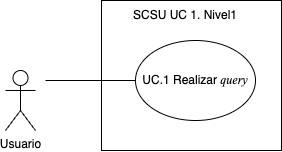
\includegraphics[width=0.4\linewidth]{images/05-desarrollo/4_ciclo/UC/SCSU_UC1_nivel1} 

}

\caption{SCSU: Diagrama de Casos de Uso 1, Nivel 1.}\label{fig:uc1}
\end{figure}

\begin{figure}

{\centering 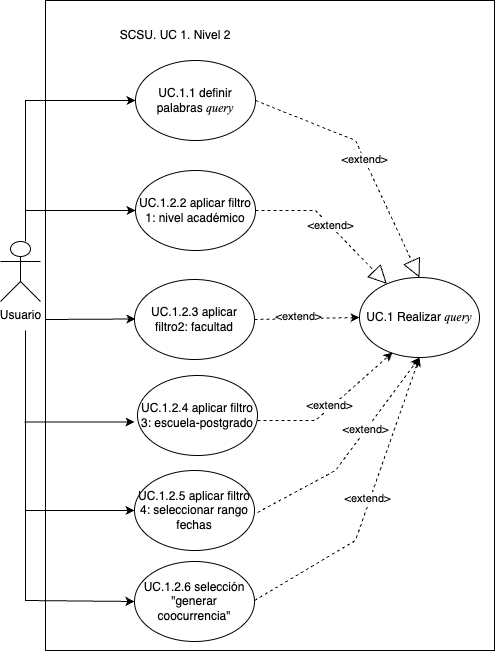
\includegraphics[width=0.5\linewidth]{images/05-desarrollo/4_ciclo/UC/SCSU_UC1_nivel2} 

}

\caption{SCSU: Diagrama de Casos de Uso 1, Nivel 1.}\label{fig:uc12}
\end{figure}

\begin{figure}

{\centering 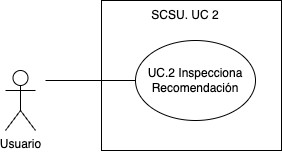
\includegraphics[width=0.4\linewidth]{images/05-desarrollo/4_ciclo/UC/SCSU_UC2_nivel1} 

}

\caption{SCSU: Diagrama de Casos de Uso 2.}\label{fig:uc2}
\end{figure}

\begin{figure}

{\centering 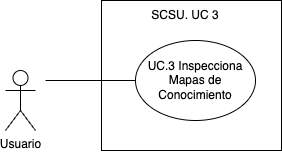
\includegraphics[width=0.4\linewidth]{images/05-desarrollo/4_ciclo/UC/SCSU_UC3_nivel1} 

}

\caption{SCSU: Diagrama de Casos de Uso 3, Nivel 1}\label{fig:uc3}
\end{figure}

\begin{figure}

{\centering 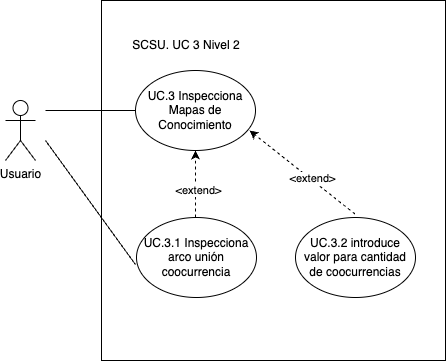
\includegraphics[width=0.5\linewidth]{images/05-desarrollo/4_ciclo/UC/SCSU_UC3_nivel2} 

}

\caption{SCSU: Diagrama de Casos de Uso 3, Nivel 2.}\label{fig:uc31}
\end{figure}

\begin{figure}

{\centering 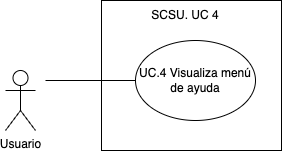
\includegraphics[width=0.4\linewidth]{images/05-desarrollo/4_ciclo/UC/SCSU_UC4} 

}

\caption{SCSU: Diagrama de Casos de Uso 4.}\label{fig:uc4}
\end{figure}

\newpage

\newpage

\global\setlength{\Oldarrayrulewidth}{\arrayrulewidth}

\global\setlength{\Oldtabcolsep}{\tabcolsep}

\setlength{\tabcolsep}{0pt}

\renewcommand*{\arraystretch}{1.5}



\providecommand{\ascline}[3]{\noalign{\global\arrayrulewidth #1}\arrayrulecolor[HTML]{#2}\cline{#3}}

\begin{longtable}[c]{|p{1.00in}|p{6.00in}}

\caption{SCSU\ UC.1.}\label{tab:tablauc1}\\

\hhline{>{\arrayrulecolor[HTML]{666666}\global\arrayrulewidth=0.75pt}->{\arrayrulecolor[HTML]{666666}\global\arrayrulewidth=0.75pt}-}

\multicolumn{1}{!{\color[HTML]{666666}\vrule width 0.75pt}>{\cellcolor[HTML]{C2C2C2}\raggedright}m{\dimexpr 1in+0\tabcolsep}}{\textcolor[HTML]{000000}{\fontsize{10}{10}\selectfont{\global\setmainfont{Helvetica}{Nombre}}}} & \multicolumn{1}{!{\color[HTML]{666666}\vrule width 0.75pt}>{\raggedright}m{\dimexpr 6in+0\tabcolsep}!{\color[HTML]{666666}\vrule width 0.75pt}}{\textcolor[HTML]{000000}{\fontsize{10}{10}\selectfont{\global\setmainfont{Helvetica}{UC.1:\ Realizar\ proceso\ de\ recuperación\ de\ información\ (query)}}}} \\

\noalign{\global\arrayrulewidth 0.75pt}\arrayrulecolor[HTML]{666666}

\hhline{|>{\arrayrulecolor[HTML]{666666}\global\arrayrulewidth=0.75pt}-|>{\arrayrulecolor[HTML]{666666}\global\arrayrulewidth=0.75pt}-}



\multicolumn{1}{!{\color[HTML]{666666}\vrule width 0.75pt}>{\cellcolor[HTML]{C2C2C2}\raggedright}m{\dimexpr 1in+0\tabcolsep}}{\textcolor[HTML]{000000}{\fontsize{10}{10}\selectfont{\global\setmainfont{Helvetica}{Descripción}}}} & \multicolumn{1}{!{\color[HTML]{666666}\vrule width 0.75pt}>{\raggedright}m{\dimexpr 6in+0\tabcolsep}!{\color[HTML]{666666}\vrule width 0.75pt}}{\textcolor[HTML]{000000}{\fontsize{10}{10}\selectfont{\global\setmainfont{Helvetica}{El\ usuario\ realiza\ búsquedas\ sobre\ los\ textos\ que\ conforman\ el\ Corpus}}}} \\

\noalign{\global\arrayrulewidth 0.75pt}\arrayrulecolor[HTML]{666666}

\hhline{|>{\arrayrulecolor[HTML]{666666}\global\arrayrulewidth=0.75pt}-|>{\arrayrulecolor[HTML]{666666}\global\arrayrulewidth=0.75pt}-}



\multicolumn{1}{!{\color[HTML]{666666}\vrule width 0.75pt}>{\cellcolor[HTML]{C2C2C2}\raggedright}m{\dimexpr 1in+0\tabcolsep}}{\textcolor[HTML]{000000}{\fontsize{10}{10}\selectfont{\global\setmainfont{Helvetica}{Actor}}}} & \multicolumn{1}{!{\color[HTML]{666666}\vrule width 0.75pt}>{\raggedright}m{\dimexpr 6in+0\tabcolsep}!{\color[HTML]{666666}\vrule width 0.75pt}}{\textcolor[HTML]{000000}{\fontsize{10}{10}\selectfont{\global\setmainfont{Helvetica}{usuario}}}} \\

\noalign{\global\arrayrulewidth 0.75pt}\arrayrulecolor[HTML]{666666}

\hhline{|>{\arrayrulecolor[HTML]{666666}\global\arrayrulewidth=0.75pt}-|>{\arrayrulecolor[HTML]{666666}\global\arrayrulewidth=0.75pt}-}



\multicolumn{2}{!{\color[HTML]{666666}\vrule width 0.75pt}>{\cellcolor[HTML]{8F8F8F}\centering}m{\dimexpr 7in+2\tabcolsep+0.75pt}!{\color[HTML]{666666}\vrule width 0.75pt}}{\textcolor[HTML]{000000}{\fontsize{10}{10}\selectfont{\global\setmainfont{Helvetica}{Flujo\ de\ Eventos}}}} \\

\noalign{\global\arrayrulewidth 0.75pt}\arrayrulecolor[HTML]{666666}

\hhline{|>{\arrayrulecolor[HTML]{666666}\global\arrayrulewidth=0.75pt}-|>{\arrayrulecolor[HTML]{666666}\global\arrayrulewidth=0.75pt}-}



\multicolumn{2}{!{\color[HTML]{666666}\vrule width 0.75pt}>{\cellcolor[HTML]{A3A3A3}\raggedright}m{\dimexpr 7in+2\tabcolsep+0.75pt}!{\color[HTML]{666666}\vrule width 0.75pt}}{\textcolor[HTML]{000000}{\fontsize{10}{10}\selectfont{\global\setmainfont{Helvetica}{Flujo\ Básico}}}} \\

\noalign{\global\arrayrulewidth 0.75pt}\arrayrulecolor[HTML]{666666}

\hhline{|>{\arrayrulecolor[HTML]{666666}\global\arrayrulewidth=0.75pt}-|>{\arrayrulecolor[HTML]{666666}\global\arrayrulewidth=0.75pt}-}



\multicolumn{2}{!{\color[HTML]{666666}\vrule width 0.75pt}>{\raggedright}m{\dimexpr 7in+2\tabcolsep+0.75pt}!{\color[HTML]{666666}\vrule width 0.75pt}}{\textcolor[HTML]{000000}{\fontsize{10}{10}\selectfont{\global\setmainfont{Helvetica}{El\ caso\ de\ uso\ inicia\ cuando\ el\ usuario\ ingresa\ a\ la\ aplicación:\ }}}\textcolor[HTML]{000000}{\fontsize{10}{10}\selectfont{\global\setmainfont{Helvetica}{\linebreak }}}\textcolor[HTML]{000000}{\fontsize{10}{10}\selectfont{\global\setmainfont{Helvetica}{\ 1)\ Introduce\ el\ texto\ a\ buscar.\ }}}\textcolor[HTML]{000000}{\fontsize{10}{10}\selectfont{\global\setmainfont{Helvetica}{\linebreak }}}\textcolor[HTML]{000000}{\fontsize{10}{10}\selectfont{\global\setmainfont{Helvetica}{\ 2)\ El\ usuario\ hace\ "clic"\ en\ "búsqueda"\ }}}\textcolor[HTML]{000000}{\fontsize{10}{10}\selectfont{\global\setmainfont{Helvetica}{\linebreak }}}\textcolor[HTML]{000000}{\fontsize{10}{10}\selectfont{\global\setmainfont{Helvetica}{\ 4)\ El\ SCSU\ presenta\ los\ resultados\ obtenidos\ }}}\textcolor[HTML]{000000}{\fontsize{10}{10}\selectfont{\global\setmainfont{Helvetica}{\linebreak }}}\textcolor[HTML]{000000}{\fontsize{10}{10}\selectfont{\global\setmainfont{Helvetica}{\ 4)\ El\ caso\ de\ uso\ termina}}}} \\

\noalign{\global\arrayrulewidth 0.75pt}\arrayrulecolor[HTML]{666666}

\hhline{|>{\arrayrulecolor[HTML]{666666}\global\arrayrulewidth=0.75pt}-|>{\arrayrulecolor[HTML]{666666}\global\arrayrulewidth=0.75pt}-}



\multicolumn{2}{!{\color[HTML]{666666}\vrule width 0.75pt}>{\cellcolor[HTML]{A3A3A3}\raggedright}m{\dimexpr 7in+2\tabcolsep+0.75pt}!{\color[HTML]{666666}\vrule width 0.75pt}}{\textcolor[HTML]{000000}{\fontsize{10}{10}\selectfont{\global\setmainfont{Helvetica}{Flujo\ Alternativo}}}} \\

\noalign{\global\arrayrulewidth 0.75pt}\arrayrulecolor[HTML]{666666}

\hhline{|>{\arrayrulecolor[HTML]{666666}\global\arrayrulewidth=0.75pt}-|>{\arrayrulecolor[HTML]{666666}\global\arrayrulewidth=0.75pt}-}



\multicolumn{1}{!{\color[HTML]{666666}\vrule width 0.75pt}>{\cellcolor[HTML]{C2C2C2}\raggedright}m{\dimexpr 1in+0\tabcolsep}}{\textcolor[HTML]{000000}{\fontsize{10}{10}\selectfont{\global\setmainfont{Helvetica}{Título}}}} & \multicolumn{1}{!{\color[HTML]{666666}\vrule width 0.75pt}>{\cellcolor[HTML]{C2C2C2}\raggedright}m{\dimexpr 6in+0\tabcolsep}!{\color[HTML]{666666}\vrule width 0.75pt}}{\textcolor[HTML]{000000}{\fontsize{10}{10}\selectfont{\global\setmainfont{Helvetica}{Descripción}}}} \\

\noalign{\global\arrayrulewidth 0.75pt}\arrayrulecolor[HTML]{666666}

\hhline{|>{\arrayrulecolor[HTML]{666666}\global\arrayrulewidth=0.75pt}-|>{\arrayrulecolor[HTML]{666666}\global\arrayrulewidth=0.75pt}-}



\multicolumn{1}{!{\color[HTML]{666666}\vrule width 0.75pt}>{\raggedright}m{\dimexpr 1in+0\tabcolsep}}{\textcolor[HTML]{000000}{\fontsize{10}{10}\selectfont{\global\setmainfont{Helvetica}{Aplica\ filtros}}}} & \multicolumn{1}{!{\color[HTML]{666666}\vrule width 0.75pt}>{\raggedright}m{\dimexpr 6in+0\tabcolsep}!{\color[HTML]{666666}\vrule width 0.75pt}}{\textcolor[HTML]{000000}{\fontsize{10}{10}\selectfont{\global\setmainfont{Helvetica}{El\ usuario\ aplica\ filtros\ para\ restringir\ la\ búsqueda}}}} \\

\noalign{\global\arrayrulewidth 0.75pt}\arrayrulecolor[HTML]{666666}

\hhline{|>{\arrayrulecolor[HTML]{666666}\global\arrayrulewidth=0.75pt}-|>{\arrayrulecolor[HTML]{666666}\global\arrayrulewidth=0.75pt}-}



\multicolumn{2}{!{\color[HTML]{666666}\vrule width 0.75pt}>{\cellcolor[HTML]{A3A3A3}\centering}m{\dimexpr 7in+2\tabcolsep+0.75pt}!{\color[HTML]{666666}\vrule width 0.75pt}}{\textcolor[HTML]{000000}{\fontsize{10}{10}\selectfont{\global\setmainfont{Helvetica}{Precondiciones}}}} \\

\noalign{\global\arrayrulewidth 0.75pt}\arrayrulecolor[HTML]{666666}

\hhline{|>{\arrayrulecolor[HTML]{666666}\global\arrayrulewidth=0.75pt}-|>{\arrayrulecolor[HTML]{666666}\global\arrayrulewidth=0.75pt}-}



\multicolumn{1}{!{\color[HTML]{666666}\vrule width 0.75pt}>{\cellcolor[HTML]{C2C2C2}\raggedright}m{\dimexpr 1in+0\tabcolsep}}{\textcolor[HTML]{000000}{\fontsize{10}{10}\selectfont{\global\setmainfont{Helvetica}{Título}}}} & \multicolumn{1}{!{\color[HTML]{666666}\vrule width 0.75pt}>{\cellcolor[HTML]{C2C2C2}\raggedright}m{\dimexpr 6in+0\tabcolsep}!{\color[HTML]{666666}\vrule width 0.75pt}}{\textcolor[HTML]{000000}{\fontsize{10}{10}\selectfont{\global\setmainfont{Helvetica}{Descripción}}}} \\

\noalign{\global\arrayrulewidth 0.75pt}\arrayrulecolor[HTML]{666666}

\hhline{|>{\arrayrulecolor[HTML]{666666}\global\arrayrulewidth=0.75pt}-|>{\arrayrulecolor[HTML]{666666}\global\arrayrulewidth=0.75pt}-}



\multicolumn{1}{!{\color[HTML]{666666}\vrule width 0.75pt}>{\raggedright}m{\dimexpr 1in+0\tabcolsep}}{\textcolor[HTML]{000000}{\fontsize{10}{10}\selectfont{\global\setmainfont{Helvetica}{N/A}}}} & \multicolumn{1}{!{\color[HTML]{666666}\vrule width 0.75pt}>{\raggedright}m{\dimexpr 6in+0\tabcolsep}!{\color[HTML]{666666}\vrule width 0.75pt}}{\textcolor[HTML]{000000}{\fontsize{10}{10}\selectfont{\global\setmainfont{Helvetica}{N/A}}}} \\

\noalign{\global\arrayrulewidth 0.75pt}\arrayrulecolor[HTML]{666666}

\hhline{|>{\arrayrulecolor[HTML]{666666}\global\arrayrulewidth=0.75pt}-|>{\arrayrulecolor[HTML]{666666}\global\arrayrulewidth=0.75pt}-}



\multicolumn{2}{!{\color[HTML]{666666}\vrule width 0.75pt}>{\cellcolor[HTML]{A3A3A3}\centering}m{\dimexpr 7in+2\tabcolsep+0.75pt}!{\color[HTML]{666666}\vrule width 0.75pt}}{\textcolor[HTML]{000000}{\fontsize{10}{10}\selectfont{\global\setmainfont{Helvetica}{Postcondiciones}}}} \\

\noalign{\global\arrayrulewidth 0.75pt}\arrayrulecolor[HTML]{666666}

\hhline{|>{\arrayrulecolor[HTML]{666666}\global\arrayrulewidth=0.75pt}-|>{\arrayrulecolor[HTML]{666666}\global\arrayrulewidth=0.75pt}-}



\multicolumn{1}{!{\color[HTML]{666666}\vrule width 0.75pt}>{\cellcolor[HTML]{C2C2C2}\raggedright}m{\dimexpr 1in+0\tabcolsep}}{\textcolor[HTML]{000000}{\fontsize{10}{10}\selectfont{\global\setmainfont{Helvetica}{Título}}}} & \multicolumn{1}{!{\color[HTML]{666666}\vrule width 0.75pt}>{\cellcolor[HTML]{C2C2C2}\raggedright}m{\dimexpr 6in+0\tabcolsep}!{\color[HTML]{666666}\vrule width 0.75pt}}{\textcolor[HTML]{000000}{\fontsize{10}{10}\selectfont{\global\setmainfont{Helvetica}{Descripción}}}} \\

\noalign{\global\arrayrulewidth 0.75pt}\arrayrulecolor[HTML]{666666}

\hhline{|>{\arrayrulecolor[HTML]{666666}\global\arrayrulewidth=0.75pt}-|>{\arrayrulecolor[HTML]{666666}\global\arrayrulewidth=0.75pt}-}



\multicolumn{1}{!{\color[HTML]{666666}\vrule width 0.75pt}>{\raggedright}m{\dimexpr 1in+0\tabcolsep}}{\textcolor[HTML]{000000}{\fontsize{10}{10}\selectfont{\global\setmainfont{Helvetica}{Éxito}}}} & \multicolumn{1}{!{\color[HTML]{666666}\vrule width 0.75pt}>{\raggedright}m{\dimexpr 6in+0\tabcolsep}!{\color[HTML]{666666}\vrule width 0.75pt}}{\textcolor[HTML]{000000}{\fontsize{10}{10}\selectfont{\global\setmainfont{Helvetica}{El\ prototipo\ presenta:\ }}}\textcolor[HTML]{000000}{\fontsize{10}{10}\selectfont{\global\setmainfont{Helvetica}{\linebreak }}}\textcolor[HTML]{000000}{\fontsize{10}{10}\selectfont{\global\setmainfont{Helvetica}{\ 1)Tabla\ con\ los\ resultados\ que\ incluye\ los\ campos\ "fecha",\ "título",\ "palabras\ claves",\ "autor",\ "facultad",\ "dependencia"\ y\ "tutor"\ \ }}}\textcolor[HTML]{000000}{\fontsize{10}{10}\selectfont{\global\setmainfont{Helvetica}{\linebreak }}}\textcolor[HTML]{000000}{\fontsize{10}{10}\selectfont{\global\setmainfont{Helvetica}{\ 2)\ Gráfico\ con\ frecuencia\ de\ aparición\ del\ texto\ del\ query\ por\ año}}}} \\

\noalign{\global\arrayrulewidth 0.75pt}\arrayrulecolor[HTML]{666666}

\hhline{|>{\arrayrulecolor[HTML]{666666}\global\arrayrulewidth=0.75pt}-|>{\arrayrulecolor[HTML]{666666}\global\arrayrulewidth=0.75pt}-}



\multicolumn{1}{!{\color[HTML]{666666}\vrule width 0.75pt}>{\raggedright}m{\dimexpr 1in+0\tabcolsep}}{\textcolor[HTML]{000000}{\fontsize{10}{10}\selectfont{\global\setmainfont{Helvetica}{Fracaso}}}} & \multicolumn{1}{!{\color[HTML]{666666}\vrule width 0.75pt}>{\raggedright}m{\dimexpr 6in+0\tabcolsep}!{\color[HTML]{666666}\vrule width 0.75pt}}{\textcolor[HTML]{000000}{\fontsize{10}{10}\selectfont{\global\setmainfont{Helvetica}{No\ presenta\ ningún\ resultado}}}} \\

\noalign{\global\arrayrulewidth 0.75pt}\arrayrulecolor[HTML]{666666}

\hhline{|>{\arrayrulecolor[HTML]{666666}\global\arrayrulewidth=0.75pt}-|>{\arrayrulecolor[HTML]{666666}\global\arrayrulewidth=0.75pt}-}



\end{longtable}



\arrayrulecolor[HTML]{000000}

\global\setlength{\arrayrulewidth}{\Oldarrayrulewidth}

\global\setlength{\tabcolsep}{\Oldtabcolsep}

\renewcommand*{\arraystretch}{1}

\newpage

\global\setlength{\Oldarrayrulewidth}{\arrayrulewidth}

\global\setlength{\Oldtabcolsep}{\tabcolsep}

\setlength{\tabcolsep}{0pt}

\renewcommand*{\arraystretch}{1.5}



\providecommand{\ascline}[3]{\noalign{\global\arrayrulewidth #1}\arrayrulecolor[HTML]{#2}\cline{#3}}

\begin{longtable}[c]{|p{1.00in}|p{6.00in}}

\caption{SCSU\ UC.1,\ Nivel\ 2.}\label{tab:tablauc11}\\

\hhline{>{\arrayrulecolor[HTML]{666666}\global\arrayrulewidth=0.75pt}->{\arrayrulecolor[HTML]{666666}\global\arrayrulewidth=0.75pt}-}

\multicolumn{1}{!{\color[HTML]{666666}\vrule width 0.75pt}>{\cellcolor[HTML]{C2C2C2}\raggedright}m{\dimexpr 1in+0\tabcolsep}}{\textcolor[HTML]{000000}{\fontsize{10}{10}\selectfont{\global\setmainfont{Helvetica}{Nombre}}}} & \multicolumn{1}{!{\color[HTML]{666666}\vrule width 0.75pt}>{\raggedright}m{\dimexpr 6in+0\tabcolsep}!{\color[HTML]{666666}\vrule width 0.75pt}}{\textcolor[HTML]{000000}{\fontsize{10}{10}\selectfont{\global\setmainfont{Helvetica}{UC.1.\ Nivel\ 2:\ Realizar\ proceso\ de\ recuperación\ de\ información\ (query)\ aplicando\ filtros.}}}} \\

\noalign{\global\arrayrulewidth 0.75pt}\arrayrulecolor[HTML]{666666}

\hhline{|>{\arrayrulecolor[HTML]{666666}\global\arrayrulewidth=0.75pt}-|>{\arrayrulecolor[HTML]{666666}\global\arrayrulewidth=0.75pt}-}



\multicolumn{1}{!{\color[HTML]{666666}\vrule width 0.75pt}>{\cellcolor[HTML]{C2C2C2}\raggedright}m{\dimexpr 1in+0\tabcolsep}}{\textcolor[HTML]{000000}{\fontsize{10}{10}\selectfont{\global\setmainfont{Helvetica}{Descripción}}}} & \multicolumn{1}{!{\color[HTML]{666666}\vrule width 0.75pt}>{\raggedright}m{\dimexpr 6in+0\tabcolsep}!{\color[HTML]{666666}\vrule width 0.75pt}}{\textcolor[HTML]{000000}{\fontsize{10}{10}\selectfont{\global\setmainfont{Helvetica}{El\ usuario\ realiza\ búsquedas\ sobre\ los\ textos\ que\ conforman\ el\ Corpus\ aplicando\ filtros}}}} \\

\noalign{\global\arrayrulewidth 0.75pt}\arrayrulecolor[HTML]{666666}

\hhline{|>{\arrayrulecolor[HTML]{666666}\global\arrayrulewidth=0.75pt}-|>{\arrayrulecolor[HTML]{666666}\global\arrayrulewidth=0.75pt}-}



\multicolumn{1}{!{\color[HTML]{666666}\vrule width 0.75pt}>{\cellcolor[HTML]{C2C2C2}\raggedright}m{\dimexpr 1in+0\tabcolsep}}{\textcolor[HTML]{000000}{\fontsize{10}{10}\selectfont{\global\setmainfont{Helvetica}{Actor}}}} & \multicolumn{1}{!{\color[HTML]{666666}\vrule width 0.75pt}>{\raggedright}m{\dimexpr 6in+0\tabcolsep}!{\color[HTML]{666666}\vrule width 0.75pt}}{\textcolor[HTML]{000000}{\fontsize{10}{10}\selectfont{\global\setmainfont{Helvetica}{usuario}}}} \\

\noalign{\global\arrayrulewidth 0.75pt}\arrayrulecolor[HTML]{666666}

\hhline{|>{\arrayrulecolor[HTML]{666666}\global\arrayrulewidth=0.75pt}-|>{\arrayrulecolor[HTML]{666666}\global\arrayrulewidth=0.75pt}-}



\multicolumn{2}{!{\color[HTML]{666666}\vrule width 0.75pt}>{\cellcolor[HTML]{8F8F8F}\centering}m{\dimexpr 7in+2\tabcolsep+0.75pt}!{\color[HTML]{666666}\vrule width 0.75pt}}{\textcolor[HTML]{000000}{\fontsize{10}{10}\selectfont{\global\setmainfont{Helvetica}{Flujo\ de\ Eventos}}}} \\

\noalign{\global\arrayrulewidth 0.75pt}\arrayrulecolor[HTML]{666666}

\hhline{|>{\arrayrulecolor[HTML]{666666}\global\arrayrulewidth=0.75pt}-|>{\arrayrulecolor[HTML]{666666}\global\arrayrulewidth=0.75pt}-}



\multicolumn{2}{!{\color[HTML]{666666}\vrule width 0.75pt}>{\cellcolor[HTML]{A3A3A3}\raggedright}m{\dimexpr 7in+2\tabcolsep+0.75pt}!{\color[HTML]{666666}\vrule width 0.75pt}}{\textcolor[HTML]{000000}{\fontsize{10}{10}\selectfont{\global\setmainfont{Helvetica}{Flujo\ Básico}}}} \\

\noalign{\global\arrayrulewidth 0.75pt}\arrayrulecolor[HTML]{666666}

\hhline{|>{\arrayrulecolor[HTML]{666666}\global\arrayrulewidth=0.75pt}-|>{\arrayrulecolor[HTML]{666666}\global\arrayrulewidth=0.75pt}-}



\multicolumn{2}{!{\color[HTML]{666666}\vrule width 0.75pt}>{\raggedright}m{\dimexpr 7in+2\tabcolsep+0.75pt}!{\color[HTML]{666666}\vrule width 0.75pt}}{\textcolor[HTML]{000000}{\fontsize{10}{10}\selectfont{\global\setmainfont{Helvetica}{El\ caso\ de\ uso\ inicia\ cuando\ el\ usuario\ ingresa\ a\ la\ aplicación\ y\ decide\ aplicar\ filtros\ al\ realizar\ la\ búsqueda.\ Los\ campos\ que\ se\ muestran\ son:\ }}}\textcolor[HTML]{000000}{\fontsize{10}{10}\selectfont{\global\setmainfont{Helvetica}{\linebreak }}}\textcolor[HTML]{000000}{\fontsize{10}{10}\selectfont{\global\setmainfont{Helvetica}{\ 1)\ Introducir\ el\ texto\ a\ buscar.\ 2)\ Filtrar\ el\ nivel\ académico.\ 3)\ Filtrar\ la\ Facultad\ \ 4)\ Filtrar\ la\ escuela\ o\ postgrado\ \ 5)\ Definir\ rango\ de\ fechas\ 6)\ Seleccionar\ "generación\ de\ coocurrencias\ (mapas\ de\ conocimiento)"\ \ 7)\ El\ usuario\ hace\ "clic"\ en\ el\ "búsqueda"\ \ 8)\ El\ SCSU\ presenta\ los\ resultados\ obtenidos\ 9)\ El\ caso\ de\ uso\ termina}}}} \\

\noalign{\global\arrayrulewidth 0.75pt}\arrayrulecolor[HTML]{666666}

\hhline{|>{\arrayrulecolor[HTML]{666666}\global\arrayrulewidth=0.75pt}-|>{\arrayrulecolor[HTML]{666666}\global\arrayrulewidth=0.75pt}-}



\multicolumn{2}{!{\color[HTML]{666666}\vrule width 0.75pt}>{\cellcolor[HTML]{A3A3A3}\raggedright}m{\dimexpr 7in+2\tabcolsep+0.75pt}!{\color[HTML]{666666}\vrule width 0.75pt}}{\textcolor[HTML]{000000}{\fontsize{10}{10}\selectfont{\global\setmainfont{Helvetica}{Flujo\ Alternativo}}}} \\

\noalign{\global\arrayrulewidth 0.75pt}\arrayrulecolor[HTML]{666666}

\hhline{|>{\arrayrulecolor[HTML]{666666}\global\arrayrulewidth=0.75pt}-|>{\arrayrulecolor[HTML]{666666}\global\arrayrulewidth=0.75pt}-}



\multicolumn{1}{!{\color[HTML]{666666}\vrule width 0.75pt}>{\cellcolor[HTML]{C2C2C2}\raggedright}m{\dimexpr 1in+0\tabcolsep}}{\textcolor[HTML]{000000}{\fontsize{10}{10}\selectfont{\global\setmainfont{Helvetica}{Título}}}} & \multicolumn{1}{!{\color[HTML]{666666}\vrule width 0.75pt}>{\cellcolor[HTML]{C2C2C2}\raggedright}m{\dimexpr 6in+0\tabcolsep}!{\color[HTML]{666666}\vrule width 0.75pt}}{\textcolor[HTML]{000000}{\fontsize{10}{10}\selectfont{\global\setmainfont{Helvetica}{Descripción}}}} \\

\noalign{\global\arrayrulewidth 0.75pt}\arrayrulecolor[HTML]{666666}

\hhline{|>{\arrayrulecolor[HTML]{666666}\global\arrayrulewidth=0.75pt}-|>{\arrayrulecolor[HTML]{666666}\global\arrayrulewidth=0.75pt}-}



\multicolumn{1}{!{\color[HTML]{666666}\vrule width 0.75pt}>{\raggedright}m{\dimexpr 1in+0\tabcolsep}}{\textcolor[HTML]{000000}{\fontsize{10}{10}\selectfont{\global\setmainfont{Helvetica}{Sin\ filtros}}}} & \multicolumn{1}{!{\color[HTML]{666666}\vrule width 0.75pt}>{\raggedright}m{\dimexpr 6in+0\tabcolsep}!{\color[HTML]{666666}\vrule width 0.75pt}}{\textcolor[HTML]{000000}{\fontsize{10}{10}\selectfont{\global\setmainfont{Helvetica}{El\ usuario\ no\ aplica\ ningún\ filtro\ y\ aparecen\ todos\ los\ resultados\ que\ contienen\ el\ texto\ de\ query}}}} \\

\noalign{\global\arrayrulewidth 0.75pt}\arrayrulecolor[HTML]{666666}

\hhline{|>{\arrayrulecolor[HTML]{666666}\global\arrayrulewidth=0.75pt}-|>{\arrayrulecolor[HTML]{666666}\global\arrayrulewidth=0.75pt}-}



\multicolumn{2}{!{\color[HTML]{666666}\vrule width 0.75pt}>{\cellcolor[HTML]{A3A3A3}\centering}m{\dimexpr 7in+2\tabcolsep+0.75pt}!{\color[HTML]{666666}\vrule width 0.75pt}}{\textcolor[HTML]{000000}{\fontsize{10}{10}\selectfont{\global\setmainfont{Helvetica}{Precondiciones}}}} \\

\noalign{\global\arrayrulewidth 0.75pt}\arrayrulecolor[HTML]{666666}

\hhline{|>{\arrayrulecolor[HTML]{666666}\global\arrayrulewidth=0.75pt}-|>{\arrayrulecolor[HTML]{666666}\global\arrayrulewidth=0.75pt}-}



\multicolumn{1}{!{\color[HTML]{666666}\vrule width 0.75pt}>{\cellcolor[HTML]{C2C2C2}\raggedright}m{\dimexpr 1in+0\tabcolsep}}{\textcolor[HTML]{000000}{\fontsize{10}{10}\selectfont{\global\setmainfont{Helvetica}{Título}}}} & \multicolumn{1}{!{\color[HTML]{666666}\vrule width 0.75pt}>{\cellcolor[HTML]{C2C2C2}\raggedright}m{\dimexpr 6in+0\tabcolsep}!{\color[HTML]{666666}\vrule width 0.75pt}}{\textcolor[HTML]{000000}{\fontsize{10}{10}\selectfont{\global\setmainfont{Helvetica}{Descripción}}}} \\

\noalign{\global\arrayrulewidth 0.75pt}\arrayrulecolor[HTML]{666666}

\hhline{|>{\arrayrulecolor[HTML]{666666}\global\arrayrulewidth=0.75pt}-|>{\arrayrulecolor[HTML]{666666}\global\arrayrulewidth=0.75pt}-}



\multicolumn{1}{!{\color[HTML]{666666}\vrule width 0.75pt}>{\raggedright}m{\dimexpr 1in+0\tabcolsep}}{\textcolor[HTML]{000000}{\fontsize{10}{10}\selectfont{\global\setmainfont{Helvetica}{N/A}}}} & \multicolumn{1}{!{\color[HTML]{666666}\vrule width 0.75pt}>{\raggedright}m{\dimexpr 6in+0\tabcolsep}!{\color[HTML]{666666}\vrule width 0.75pt}}{\textcolor[HTML]{000000}{\fontsize{10}{10}\selectfont{\global\setmainfont{Helvetica}{N/A}}}} \\

\noalign{\global\arrayrulewidth 0.75pt}\arrayrulecolor[HTML]{666666}

\hhline{|>{\arrayrulecolor[HTML]{666666}\global\arrayrulewidth=0.75pt}-|>{\arrayrulecolor[HTML]{666666}\global\arrayrulewidth=0.75pt}-}



\multicolumn{2}{!{\color[HTML]{666666}\vrule width 0.75pt}>{\cellcolor[HTML]{A3A3A3}\centering}m{\dimexpr 7in+2\tabcolsep+0.75pt}!{\color[HTML]{666666}\vrule width 0.75pt}}{\textcolor[HTML]{000000}{\fontsize{10}{10}\selectfont{\global\setmainfont{Helvetica}{Postcondiciones}}}} \\

\noalign{\global\arrayrulewidth 0.75pt}\arrayrulecolor[HTML]{666666}

\hhline{|>{\arrayrulecolor[HTML]{666666}\global\arrayrulewidth=0.75pt}-|>{\arrayrulecolor[HTML]{666666}\global\arrayrulewidth=0.75pt}-}



\multicolumn{1}{!{\color[HTML]{666666}\vrule width 0.75pt}>{\cellcolor[HTML]{C2C2C2}\raggedright}m{\dimexpr 1in+0\tabcolsep}}{\textcolor[HTML]{000000}{\fontsize{10}{10}\selectfont{\global\setmainfont{Helvetica}{Título}}}} & \multicolumn{1}{!{\color[HTML]{666666}\vrule width 0.75pt}>{\cellcolor[HTML]{C2C2C2}\raggedright}m{\dimexpr 6in+0\tabcolsep}!{\color[HTML]{666666}\vrule width 0.75pt}}{\textcolor[HTML]{000000}{\fontsize{10}{10}\selectfont{\global\setmainfont{Helvetica}{Descripción}}}} \\

\noalign{\global\arrayrulewidth 0.75pt}\arrayrulecolor[HTML]{666666}

\hhline{|>{\arrayrulecolor[HTML]{666666}\global\arrayrulewidth=0.75pt}-|>{\arrayrulecolor[HTML]{666666}\global\arrayrulewidth=0.75pt}-}



\multicolumn{1}{!{\color[HTML]{666666}\vrule width 0.75pt}>{\raggedright}m{\dimexpr 1in+0\tabcolsep}}{\textcolor[HTML]{000000}{\fontsize{10}{10}\selectfont{\global\setmainfont{Helvetica}{Éxito}}}} & \multicolumn{1}{!{\color[HTML]{666666}\vrule width 0.75pt}>{\raggedright}m{\dimexpr 6in+0\tabcolsep}!{\color[HTML]{666666}\vrule width 0.75pt}}{\textcolor[HTML]{000000}{\fontsize{10}{10}\selectfont{\global\setmainfont{Helvetica}{El\ SCSU\ presenta:\ }}}\textcolor[HTML]{000000}{\fontsize{10}{10}\selectfont{\global\setmainfont{Helvetica}{\linebreak }}}\textcolor[HTML]{000000}{\fontsize{10}{10}\selectfont{\global\setmainfont{Helvetica}{\ 1)Tabla\ con\ los\ resultados\ que\ incluye\ los\ campos\ "fecha",\ "título",\ "palabras\ claves",\ "autor",\ "facultad",\ "dependencia"\ y\ "tutor"\ \ }}}\textcolor[HTML]{000000}{\fontsize{10}{10}\selectfont{\global\setmainfont{Helvetica}{\linebreak }}}\textcolor[HTML]{000000}{\fontsize{10}{10}\selectfont{\global\setmainfont{Helvetica}{\ 3)\ Gráfico\ con\ frecuencia\ de\ aparición\ del\ texto\ del\ query\ por\ año\ }}}\textcolor[HTML]{000000}{\fontsize{10}{10}\selectfont{\global\setmainfont{Helvetica}{\linebreak }}}\textcolor[HTML]{000000}{\fontsize{10}{10}\selectfont{\global\setmainfont{Helvetica}{\ 4)\ Gráfico\ con\ "Mapas\ de\ Conocimiento"}}}} \\

\noalign{\global\arrayrulewidth 0.75pt}\arrayrulecolor[HTML]{666666}

\hhline{|>{\arrayrulecolor[HTML]{666666}\global\arrayrulewidth=0.75pt}-|>{\arrayrulecolor[HTML]{666666}\global\arrayrulewidth=0.75pt}-}



\multicolumn{1}{!{\color[HTML]{666666}\vrule width 0.75pt}>{\raggedright}m{\dimexpr 1in+0\tabcolsep}}{\textcolor[HTML]{000000}{\fontsize{10}{10}\selectfont{\global\setmainfont{Helvetica}{Fracaso}}}} & \multicolumn{1}{!{\color[HTML]{666666}\vrule width 0.75pt}>{\raggedright}m{\dimexpr 6in+0\tabcolsep}!{\color[HTML]{666666}\vrule width 0.75pt}}{\textcolor[HTML]{000000}{\fontsize{10}{10}\selectfont{\global\setmainfont{Helvetica}{No\ presenta\ ningún\ resultado}}}} \\

\noalign{\global\arrayrulewidth 0.75pt}\arrayrulecolor[HTML]{666666}

\hhline{|>{\arrayrulecolor[HTML]{666666}\global\arrayrulewidth=0.75pt}-|>{\arrayrulecolor[HTML]{666666}\global\arrayrulewidth=0.75pt}-}



\end{longtable}



\arrayrulecolor[HTML]{000000}

\global\setlength{\arrayrulewidth}{\Oldarrayrulewidth}

\global\setlength{\tabcolsep}{\Oldtabcolsep}

\renewcommand*{\arraystretch}{1}

\newpage

\global\setlength{\Oldarrayrulewidth}{\arrayrulewidth}

\global\setlength{\Oldtabcolsep}{\tabcolsep}

\setlength{\tabcolsep}{0pt}

\renewcommand*{\arraystretch}{1.5}



\providecommand{\ascline}[3]{\noalign{\global\arrayrulewidth #1}\arrayrulecolor[HTML]{#2}\cline{#3}}

\begin{longtable}[c]{|p{1.00in}|p{6.00in}}

\caption{SCSU\ UC.\ 2.}\label{tab:tablauc2}\\

\hhline{>{\arrayrulecolor[HTML]{666666}\global\arrayrulewidth=0.75pt}->{\arrayrulecolor[HTML]{666666}\global\arrayrulewidth=0.75pt}-}

\multicolumn{1}{!{\color[HTML]{666666}\vrule width 0.75pt}>{\cellcolor[HTML]{C2C2C2}\raggedright}m{\dimexpr 1in+0\tabcolsep}}{\textcolor[HTML]{000000}{\fontsize{10}{10}\selectfont{\global\setmainfont{Helvetica}{Nombre}}}} & \multicolumn{1}{!{\color[HTML]{666666}\vrule width 0.75pt}>{\raggedright}m{\dimexpr 6in+0\tabcolsep}!{\color[HTML]{666666}\vrule width 0.75pt}}{\textcolor[HTML]{000000}{\fontsize{10}{10}\selectfont{\global\setmainfont{Helvetica}{UC.2:\ Realizar\ Inspección\ de\ Recomendaciones}}}} \\

\noalign{\global\arrayrulewidth 0.75pt}\arrayrulecolor[HTML]{666666}

\hhline{|>{\arrayrulecolor[HTML]{666666}\global\arrayrulewidth=0.75pt}-|>{\arrayrulecolor[HTML]{666666}\global\arrayrulewidth=0.75pt}-}



\multicolumn{1}{!{\color[HTML]{666666}\vrule width 0.75pt}>{\cellcolor[HTML]{C2C2C2}\raggedright}m{\dimexpr 1in+0\tabcolsep}}{\textcolor[HTML]{000000}{\fontsize{10}{10}\selectfont{\global\setmainfont{Helvetica}{Descripción}}}} & \multicolumn{1}{!{\color[HTML]{666666}\vrule width 0.75pt}>{\raggedright}m{\dimexpr 6in+0\tabcolsep}!{\color[HTML]{666666}\vrule width 0.75pt}}{\textcolor[HTML]{000000}{\fontsize{10}{10}\selectfont{\global\setmainfont{Helvetica}{El\ usuario\ inspecciona\ un\ documento\ de\ interés\ haciendo\ "clic"\ y\ se\ muestran\ las\ títulos\ y\ vínculos\ a\ investigaciones\ recomendadas}}}} \\

\noalign{\global\arrayrulewidth 0.75pt}\arrayrulecolor[HTML]{666666}

\hhline{|>{\arrayrulecolor[HTML]{666666}\global\arrayrulewidth=0.75pt}-|>{\arrayrulecolor[HTML]{666666}\global\arrayrulewidth=0.75pt}-}



\multicolumn{1}{!{\color[HTML]{666666}\vrule width 0.75pt}>{\cellcolor[HTML]{C2C2C2}\raggedright}m{\dimexpr 1in+0\tabcolsep}}{\textcolor[HTML]{000000}{\fontsize{10}{10}\selectfont{\global\setmainfont{Helvetica}{Actor}}}} & \multicolumn{1}{!{\color[HTML]{666666}\vrule width 0.75pt}>{\raggedright}m{\dimexpr 6in+0\tabcolsep}!{\color[HTML]{666666}\vrule width 0.75pt}}{\textcolor[HTML]{000000}{\fontsize{10}{10}\selectfont{\global\setmainfont{Helvetica}{usuario}}}} \\

\noalign{\global\arrayrulewidth 0.75pt}\arrayrulecolor[HTML]{666666}

\hhline{|>{\arrayrulecolor[HTML]{666666}\global\arrayrulewidth=0.75pt}-|>{\arrayrulecolor[HTML]{666666}\global\arrayrulewidth=0.75pt}-}



\multicolumn{2}{!{\color[HTML]{666666}\vrule width 0.75pt}>{\cellcolor[HTML]{8F8F8F}\centering}m{\dimexpr 7in+2\tabcolsep+0.75pt}!{\color[HTML]{666666}\vrule width 0.75pt}}{\textcolor[HTML]{000000}{\fontsize{10}{10}\selectfont{\global\setmainfont{Helvetica}{Flujo\ de\ Eventos}}}} \\

\noalign{\global\arrayrulewidth 0.75pt}\arrayrulecolor[HTML]{666666}

\hhline{|>{\arrayrulecolor[HTML]{666666}\global\arrayrulewidth=0.75pt}-|>{\arrayrulecolor[HTML]{666666}\global\arrayrulewidth=0.75pt}-}



\multicolumn{2}{!{\color[HTML]{666666}\vrule width 0.75pt}>{\cellcolor[HTML]{A3A3A3}\raggedright}m{\dimexpr 7in+2\tabcolsep+0.75pt}!{\color[HTML]{666666}\vrule width 0.75pt}}{\textcolor[HTML]{000000}{\fontsize{10}{10}\selectfont{\global\setmainfont{Helvetica}{Flujo\ Básico}}}} \\

\noalign{\global\arrayrulewidth 0.75pt}\arrayrulecolor[HTML]{666666}

\hhline{|>{\arrayrulecolor[HTML]{666666}\global\arrayrulewidth=0.75pt}-|>{\arrayrulecolor[HTML]{666666}\global\arrayrulewidth=0.75pt}-}



\multicolumn{2}{!{\color[HTML]{666666}\vrule width 0.75pt}>{\raggedright}m{\dimexpr 7in+2\tabcolsep+0.75pt}!{\color[HTML]{666666}\vrule width 0.75pt}}{\textcolor[HTML]{000000}{\fontsize{10}{10}\selectfont{\global\setmainfont{Helvetica}{El\ caso\ de\ uso\ inicia\ cuando\ }}}\textcolor[HTML]{000000}{\fontsize{10}{10}\selectfont{\global\setmainfont{Helvetica}{\linebreak }}}\textcolor[HTML]{000000}{\fontsize{10}{10}\selectfont{\global\setmainfont{Helvetica}{\ 1)\ el\ usuario\ inspecciona\ la\ tabla\ con\ los\ resultados\ de\ la\ búsqueda\ y\ hace\ "clic"\ sobre\ una\ fila\ y\ se\ expande\ la\ fila\ asociada\ a\ una\ investigación.\ }}}\textcolor[HTML]{000000}{\fontsize{10}{10}\selectfont{\global\setmainfont{Helvetica}{\linebreak }}}\textcolor[HTML]{000000}{\fontsize{10}{10}\selectfont{\global\setmainfont{Helvetica}{\ 2)\ el\ caso\ de\ uso\ termina}}}} \\

\noalign{\global\arrayrulewidth 0.75pt}\arrayrulecolor[HTML]{666666}

\hhline{|>{\arrayrulecolor[HTML]{666666}\global\arrayrulewidth=0.75pt}-|>{\arrayrulecolor[HTML]{666666}\global\arrayrulewidth=0.75pt}-}



\multicolumn{2}{!{\color[HTML]{666666}\vrule width 0.75pt}>{\cellcolor[HTML]{A3A3A3}\raggedright}m{\dimexpr 7in+2\tabcolsep+0.75pt}!{\color[HTML]{666666}\vrule width 0.75pt}}{\textcolor[HTML]{000000}{\fontsize{10}{10}\selectfont{\global\setmainfont{Helvetica}{Flujo\ Alternativo}}}} \\

\noalign{\global\arrayrulewidth 0.75pt}\arrayrulecolor[HTML]{666666}

\hhline{|>{\arrayrulecolor[HTML]{666666}\global\arrayrulewidth=0.75pt}-|>{\arrayrulecolor[HTML]{666666}\global\arrayrulewidth=0.75pt}-}



\multicolumn{1}{!{\color[HTML]{666666}\vrule width 0.75pt}>{\cellcolor[HTML]{C2C2C2}\raggedright}m{\dimexpr 1in+0\tabcolsep}}{\textcolor[HTML]{000000}{\fontsize{10}{10}\selectfont{\global\setmainfont{Helvetica}{Título}}}} & \multicolumn{1}{!{\color[HTML]{666666}\vrule width 0.75pt}>{\cellcolor[HTML]{C2C2C2}\raggedright}m{\dimexpr 6in+0\tabcolsep}!{\color[HTML]{666666}\vrule width 0.75pt}}{\textcolor[HTML]{000000}{\fontsize{10}{10}\selectfont{\global\setmainfont{Helvetica}{Descripción}}}} \\

\noalign{\global\arrayrulewidth 0.75pt}\arrayrulecolor[HTML]{666666}

\hhline{|>{\arrayrulecolor[HTML]{666666}\global\arrayrulewidth=0.75pt}-|>{\arrayrulecolor[HTML]{666666}\global\arrayrulewidth=0.75pt}-}



\multicolumn{1}{!{\color[HTML]{666666}\vrule width 0.75pt}>{\raggedright}m{\dimexpr 1in+0\tabcolsep}}{\textcolor[HTML]{000000}{\fontsize{10}{10}\selectfont{\global\setmainfont{Helvetica}{no\ inspecciona}}}} & \multicolumn{1}{!{\color[HTML]{666666}\vrule width 0.75pt}>{\raggedright}m{\dimexpr 6in+0\tabcolsep}!{\color[HTML]{666666}\vrule width 0.75pt}}{\textcolor[HTML]{000000}{\fontsize{10}{10}\selectfont{\global\setmainfont{Helvetica}{No\ se\ despliega\ el\ área\ que\ muestra\ las\ recomendaciones}}}} \\

\noalign{\global\arrayrulewidth 0.75pt}\arrayrulecolor[HTML]{666666}

\hhline{|>{\arrayrulecolor[HTML]{666666}\global\arrayrulewidth=0.75pt}-|>{\arrayrulecolor[HTML]{666666}\global\arrayrulewidth=0.75pt}-}



\multicolumn{2}{!{\color[HTML]{666666}\vrule width 0.75pt}>{\cellcolor[HTML]{A3A3A3}\centering}m{\dimexpr 7in+2\tabcolsep+0.75pt}!{\color[HTML]{666666}\vrule width 0.75pt}}{\textcolor[HTML]{000000}{\fontsize{10}{10}\selectfont{\global\setmainfont{Helvetica}{Precondiciones}}}} \\

\noalign{\global\arrayrulewidth 0.75pt}\arrayrulecolor[HTML]{666666}

\hhline{|>{\arrayrulecolor[HTML]{666666}\global\arrayrulewidth=0.75pt}-|>{\arrayrulecolor[HTML]{666666}\global\arrayrulewidth=0.75pt}-}



\multicolumn{1}{!{\color[HTML]{666666}\vrule width 0.75pt}>{\cellcolor[HTML]{C2C2C2}\raggedright}m{\dimexpr 1in+0\tabcolsep}}{\textcolor[HTML]{000000}{\fontsize{10}{10}\selectfont{\global\setmainfont{Helvetica}{Título}}}} & \multicolumn{1}{!{\color[HTML]{666666}\vrule width 0.75pt}>{\cellcolor[HTML]{C2C2C2}\raggedright}m{\dimexpr 6in+0\tabcolsep}!{\color[HTML]{666666}\vrule width 0.75pt}}{\textcolor[HTML]{000000}{\fontsize{10}{10}\selectfont{\global\setmainfont{Helvetica}{Descripción}}}} \\

\noalign{\global\arrayrulewidth 0.75pt}\arrayrulecolor[HTML]{666666}

\hhline{|>{\arrayrulecolor[HTML]{666666}\global\arrayrulewidth=0.75pt}-|>{\arrayrulecolor[HTML]{666666}\global\arrayrulewidth=0.75pt}-}



\multicolumn{1}{!{\color[HTML]{666666}\vrule width 0.75pt}>{\raggedright}m{\dimexpr 1in+0\tabcolsep}}{\textcolor[HTML]{000000}{\fontsize{10}{10}\selectfont{\global\setmainfont{Helvetica}{Realizar\ query}}}} & \multicolumn{1}{!{\color[HTML]{666666}\vrule width 0.75pt}>{\raggedright}m{\dimexpr 6in+0\tabcolsep}!{\color[HTML]{666666}\vrule width 0.75pt}}{\textcolor[HTML]{000000}{\fontsize{10}{10}\selectfont{\global\setmainfont{Helvetica}{Haber\ realizado\ el\ UC.\ 1.}}}} \\

\noalign{\global\arrayrulewidth 0.75pt}\arrayrulecolor[HTML]{666666}

\hhline{|>{\arrayrulecolor[HTML]{666666}\global\arrayrulewidth=0.75pt}-|>{\arrayrulecolor[HTML]{666666}\global\arrayrulewidth=0.75pt}-}



\multicolumn{2}{!{\color[HTML]{666666}\vrule width 0.75pt}>{\cellcolor[HTML]{A3A3A3}\centering}m{\dimexpr 7in+2\tabcolsep+0.75pt}!{\color[HTML]{666666}\vrule width 0.75pt}}{\textcolor[HTML]{000000}{\fontsize{10}{10}\selectfont{\global\setmainfont{Helvetica}{Postcondiciones}}}} \\

\noalign{\global\arrayrulewidth 0.75pt}\arrayrulecolor[HTML]{666666}

\hhline{|>{\arrayrulecolor[HTML]{666666}\global\arrayrulewidth=0.75pt}-|>{\arrayrulecolor[HTML]{666666}\global\arrayrulewidth=0.75pt}-}



\multicolumn{1}{!{\color[HTML]{666666}\vrule width 0.75pt}>{\cellcolor[HTML]{C2C2C2}\raggedright}m{\dimexpr 1in+0\tabcolsep}}{\textcolor[HTML]{000000}{\fontsize{10}{10}\selectfont{\global\setmainfont{Helvetica}{Título}}}} & \multicolumn{1}{!{\color[HTML]{666666}\vrule width 0.75pt}>{\cellcolor[HTML]{C2C2C2}\raggedright}m{\dimexpr 6in+0\tabcolsep}!{\color[HTML]{666666}\vrule width 0.75pt}}{\textcolor[HTML]{000000}{\fontsize{10}{10}\selectfont{\global\setmainfont{Helvetica}{Descripción}}}} \\

\noalign{\global\arrayrulewidth 0.75pt}\arrayrulecolor[HTML]{666666}

\hhline{|>{\arrayrulecolor[HTML]{666666}\global\arrayrulewidth=0.75pt}-|>{\arrayrulecolor[HTML]{666666}\global\arrayrulewidth=0.75pt}-}



\multicolumn{1}{!{\color[HTML]{666666}\vrule width 0.75pt}>{\raggedright}m{\dimexpr 1in+0\tabcolsep}}{\textcolor[HTML]{000000}{\fontsize{10}{10}\selectfont{\global\setmainfont{Helvetica}{Éxito}}}} & \multicolumn{1}{!{\color[HTML]{666666}\vrule width 0.75pt}>{\raggedright}m{\dimexpr 6in+0\tabcolsep}!{\color[HTML]{666666}\vrule width 0.75pt}}{\textcolor[HTML]{000000}{\fontsize{10}{10}\selectfont{\global\setmainfont{Helvetica}{El\ SCSU\ presenta:\ }}}\textcolor[HTML]{000000}{\fontsize{10}{10}\selectfont{\global\setmainfont{Helvetica}{\linebreak }}}\textcolor[HTML]{000000}{\fontsize{10}{10}\selectfont{\global\setmainfont{Helvetica}{\ 1)\ listado\ con\ hasta\ cinco\ títulos\ de\ documentos\ recomendados\ que\ contienen\ el\ hipervínculo\ a\ la\ investigación\ alojada\ en\ Saber\ UCV\ }}}} \\

\noalign{\global\arrayrulewidth 0.75pt}\arrayrulecolor[HTML]{666666}

\hhline{|>{\arrayrulecolor[HTML]{666666}\global\arrayrulewidth=0.75pt}-|>{\arrayrulecolor[HTML]{666666}\global\arrayrulewidth=0.75pt}-}



\multicolumn{1}{!{\color[HTML]{666666}\vrule width 0.75pt}>{\raggedright}m{\dimexpr 1in+0\tabcolsep}}{\textcolor[HTML]{000000}{\fontsize{10}{10}\selectfont{\global\setmainfont{Helvetica}{Fracaso}}}} & \multicolumn{1}{!{\color[HTML]{666666}\vrule width 0.75pt}>{\raggedright}m{\dimexpr 6in+0\tabcolsep}!{\color[HTML]{666666}\vrule width 0.75pt}}{\textcolor[HTML]{000000}{\fontsize{10}{10}\selectfont{\global\setmainfont{Helvetica}{No\ se\ muestran\ recomendaciones\ por\ no\ disponer\ de\ documentos\ similares\ en\ el\ Corpus}}}} \\

\noalign{\global\arrayrulewidth 0.75pt}\arrayrulecolor[HTML]{666666}

\hhline{|>{\arrayrulecolor[HTML]{666666}\global\arrayrulewidth=0.75pt}-|>{\arrayrulecolor[HTML]{666666}\global\arrayrulewidth=0.75pt}-}



\end{longtable}



\arrayrulecolor[HTML]{000000}

\global\setlength{\arrayrulewidth}{\Oldarrayrulewidth}

\global\setlength{\tabcolsep}{\Oldtabcolsep}

\renewcommand*{\arraystretch}{1}

\newpage

\global\setlength{\Oldarrayrulewidth}{\arrayrulewidth}

\global\setlength{\Oldtabcolsep}{\tabcolsep}

\setlength{\tabcolsep}{0pt}

\renewcommand*{\arraystretch}{1.5}



\providecommand{\ascline}[3]{\noalign{\global\arrayrulewidth #1}\arrayrulecolor[HTML]{#2}\cline{#3}}

\begin{longtable}[c]{|p{1.00in}|p{6.00in}}

\caption{SCSU\ UC.\ 3.}\label{tab:tablauc3}\\

\hhline{>{\arrayrulecolor[HTML]{666666}\global\arrayrulewidth=0.75pt}->{\arrayrulecolor[HTML]{666666}\global\arrayrulewidth=0.75pt}-}

\multicolumn{1}{!{\color[HTML]{666666}\vrule width 0.75pt}>{\cellcolor[HTML]{C2C2C2}\raggedright}m{\dimexpr 1in+0\tabcolsep}}{\textcolor[HTML]{000000}{\fontsize{10}{10}\selectfont{\global\setmainfont{Helvetica}{Nombre}}}} & \multicolumn{1}{!{\color[HTML]{666666}\vrule width 0.75pt}>{\raggedright}m{\dimexpr 6in+0\tabcolsep}!{\color[HTML]{666666}\vrule width 0.75pt}}{\textcolor[HTML]{000000}{\fontsize{10}{10}\selectfont{\global\setmainfont{Helvetica}{UC.3:\ Realizar\ inspección\ de\ "Mapas\ de\ Conocimiento"}}}} \\

\noalign{\global\arrayrulewidth 0.75pt}\arrayrulecolor[HTML]{666666}

\hhline{|>{\arrayrulecolor[HTML]{666666}\global\arrayrulewidth=0.75pt}-|>{\arrayrulecolor[HTML]{666666}\global\arrayrulewidth=0.75pt}-}



\multicolumn{1}{!{\color[HTML]{666666}\vrule width 0.75pt}>{\cellcolor[HTML]{C2C2C2}\raggedright}m{\dimexpr 1in+0\tabcolsep}}{\textcolor[HTML]{000000}{\fontsize{10}{10}\selectfont{\global\setmainfont{Helvetica}{Descripción}}}} & \multicolumn{1}{!{\color[HTML]{666666}\vrule width 0.75pt}>{\raggedright}m{\dimexpr 6in+0\tabcolsep}!{\color[HTML]{666666}\vrule width 0.75pt}}{\textcolor[HTML]{000000}{\fontsize{10}{10}\selectfont{\global\setmainfont{Helvetica}{El\ usuario\ revisa\ los\ "Mapas\ de\ Conocimiento"\ generados\ con\ los\ documentos\ que\ fueron\ recuperados\ en\ el\ query}}}} \\

\noalign{\global\arrayrulewidth 0.75pt}\arrayrulecolor[HTML]{666666}

\hhline{|>{\arrayrulecolor[HTML]{666666}\global\arrayrulewidth=0.75pt}-|>{\arrayrulecolor[HTML]{666666}\global\arrayrulewidth=0.75pt}-}



\multicolumn{1}{!{\color[HTML]{666666}\vrule width 0.75pt}>{\cellcolor[HTML]{C2C2C2}\raggedright}m{\dimexpr 1in+0\tabcolsep}}{\textcolor[HTML]{000000}{\fontsize{10}{10}\selectfont{\global\setmainfont{Helvetica}{Actor}}}} & \multicolumn{1}{!{\color[HTML]{666666}\vrule width 0.75pt}>{\raggedright}m{\dimexpr 6in+0\tabcolsep}!{\color[HTML]{666666}\vrule width 0.75pt}}{\textcolor[HTML]{000000}{\fontsize{10}{10}\selectfont{\global\setmainfont{Helvetica}{usuario}}}} \\

\noalign{\global\arrayrulewidth 0.75pt}\arrayrulecolor[HTML]{666666}

\hhline{|>{\arrayrulecolor[HTML]{666666}\global\arrayrulewidth=0.75pt}-|>{\arrayrulecolor[HTML]{666666}\global\arrayrulewidth=0.75pt}-}



\multicolumn{2}{!{\color[HTML]{666666}\vrule width 0.75pt}>{\cellcolor[HTML]{8F8F8F}\centering}m{\dimexpr 7in+2\tabcolsep+0.75pt}!{\color[HTML]{666666}\vrule width 0.75pt}}{\textcolor[HTML]{000000}{\fontsize{10}{10}\selectfont{\global\setmainfont{Helvetica}{Flujo\ de\ Eventos}}}} \\

\noalign{\global\arrayrulewidth 0.75pt}\arrayrulecolor[HTML]{666666}

\hhline{|>{\arrayrulecolor[HTML]{666666}\global\arrayrulewidth=0.75pt}-|>{\arrayrulecolor[HTML]{666666}\global\arrayrulewidth=0.75pt}-}



\multicolumn{2}{!{\color[HTML]{666666}\vrule width 0.75pt}>{\cellcolor[HTML]{A3A3A3}\raggedright}m{\dimexpr 7in+2\tabcolsep+0.75pt}!{\color[HTML]{666666}\vrule width 0.75pt}}{\textcolor[HTML]{000000}{\fontsize{10}{10}\selectfont{\global\setmainfont{Helvetica}{Flujo\ Básico}}}} \\

\noalign{\global\arrayrulewidth 0.75pt}\arrayrulecolor[HTML]{666666}

\hhline{|>{\arrayrulecolor[HTML]{666666}\global\arrayrulewidth=0.75pt}-|>{\arrayrulecolor[HTML]{666666}\global\arrayrulewidth=0.75pt}-}



\multicolumn{2}{!{\color[HTML]{666666}\vrule width 0.75pt}>{\raggedright}m{\dimexpr 7in+2\tabcolsep+0.75pt}!{\color[HTML]{666666}\vrule width 0.75pt}}{\textcolor[HTML]{000000}{\fontsize{10}{10}\selectfont{\global\setmainfont{Helvetica}{El\ caso\ de\ uso\ inicia\ cuando\ el\ usuario:\ }}}\textcolor[HTML]{000000}{\fontsize{10}{10}\selectfont{\global\setmainfont{Helvetica}{\linebreak }}}\textcolor[HTML]{000000}{\fontsize{10}{10}\selectfont{\global\setmainfont{Helvetica}{\ 1)\ Hace\ "clic"\ en\ la\ pestaña\ de\ nombre\ "Coocurrencias".\ }}}\textcolor[HTML]{000000}{\fontsize{10}{10}\selectfont{\global\setmainfont{Helvetica}{\linebreak }}}\textcolor[HTML]{000000}{\fontsize{10}{10}\selectfont{\global\setmainfont{Helvetica}{\ 2)\ Se\ muestra\ un\ gráfico\ interactivo\ con\ los\ "Mapas\ de\ Conocimiento"\ generados.\ }}}\textcolor[HTML]{000000}{\fontsize{10}{10}\selectfont{\global\setmainfont{Helvetica}{\linebreak }}}\textcolor[HTML]{000000}{\fontsize{10}{10}\selectfont{\global\setmainfont{Helvetica}{\ 3)\ El\ caso\ de\ uso\ termina}}}} \\

\noalign{\global\arrayrulewidth 0.75pt}\arrayrulecolor[HTML]{666666}

\hhline{|>{\arrayrulecolor[HTML]{666666}\global\arrayrulewidth=0.75pt}-|>{\arrayrulecolor[HTML]{666666}\global\arrayrulewidth=0.75pt}-}



\multicolumn{2}{!{\color[HTML]{666666}\vrule width 0.75pt}>{\cellcolor[HTML]{A3A3A3}\raggedright}m{\dimexpr 7in+2\tabcolsep+0.75pt}!{\color[HTML]{666666}\vrule width 0.75pt}}{\textcolor[HTML]{000000}{\fontsize{10}{10}\selectfont{\global\setmainfont{Helvetica}{Flujo\ Alternativo}}}} \\

\noalign{\global\arrayrulewidth 0.75pt}\arrayrulecolor[HTML]{666666}

\hhline{|>{\arrayrulecolor[HTML]{666666}\global\arrayrulewidth=0.75pt}-|>{\arrayrulecolor[HTML]{666666}\global\arrayrulewidth=0.75pt}-}



\multicolumn{1}{!{\color[HTML]{666666}\vrule width 0.75pt}>{\cellcolor[HTML]{C2C2C2}\raggedright}m{\dimexpr 1in+0\tabcolsep}}{\textcolor[HTML]{000000}{\fontsize{10}{10}\selectfont{\global\setmainfont{Helvetica}{Título}}}} & \multicolumn{1}{!{\color[HTML]{666666}\vrule width 0.75pt}>{\cellcolor[HTML]{C2C2C2}\raggedright}m{\dimexpr 6in+0\tabcolsep}!{\color[HTML]{666666}\vrule width 0.75pt}}{\textcolor[HTML]{000000}{\fontsize{10}{10}\selectfont{\global\setmainfont{Helvetica}{Descripción}}}} \\

\noalign{\global\arrayrulewidth 0.75pt}\arrayrulecolor[HTML]{666666}

\hhline{|>{\arrayrulecolor[HTML]{666666}\global\arrayrulewidth=0.75pt}-|>{\arrayrulecolor[HTML]{666666}\global\arrayrulewidth=0.75pt}-}



\multicolumn{1}{!{\color[HTML]{666666}\vrule width 0.75pt}>{\raggedright}m{\dimexpr 1in+0\tabcolsep}}{\textcolor[HTML]{000000}{\fontsize{10}{10}\selectfont{\global\setmainfont{Helvetica}{Sin\ Coocurrencia}}}} & \multicolumn{1}{!{\color[HTML]{666666}\vrule width 0.75pt}>{\raggedright}m{\dimexpr 6in+0\tabcolsep}!{\color[HTML]{666666}\vrule width 0.75pt}}{\textcolor[HTML]{000000}{\fontsize{10}{10}\selectfont{\global\setmainfont{Helvetica}{El\ usuario\ no\ selecciona\ la\ ventana\ "coocurrencia"\ y\ no\ se\ muestran\ los\ "Mapas\ de\ Conocimiento"}}}} \\

\noalign{\global\arrayrulewidth 0.75pt}\arrayrulecolor[HTML]{666666}

\hhline{|>{\arrayrulecolor[HTML]{666666}\global\arrayrulewidth=0.75pt}-|>{\arrayrulecolor[HTML]{666666}\global\arrayrulewidth=0.75pt}-}



\multicolumn{2}{!{\color[HTML]{666666}\vrule width 0.75pt}>{\cellcolor[HTML]{A3A3A3}\centering}m{\dimexpr 7in+2\tabcolsep+0.75pt}!{\color[HTML]{666666}\vrule width 0.75pt}}{\textcolor[HTML]{000000}{\fontsize{10}{10}\selectfont{\global\setmainfont{Helvetica}{Precondiciones}}}} \\

\noalign{\global\arrayrulewidth 0.75pt}\arrayrulecolor[HTML]{666666}

\hhline{|>{\arrayrulecolor[HTML]{666666}\global\arrayrulewidth=0.75pt}-|>{\arrayrulecolor[HTML]{666666}\global\arrayrulewidth=0.75pt}-}



\multicolumn{1}{!{\color[HTML]{666666}\vrule width 0.75pt}>{\cellcolor[HTML]{C2C2C2}\raggedright}m{\dimexpr 1in+0\tabcolsep}}{\textcolor[HTML]{000000}{\fontsize{10}{10}\selectfont{\global\setmainfont{Helvetica}{Título}}}} & \multicolumn{1}{!{\color[HTML]{666666}\vrule width 0.75pt}>{\cellcolor[HTML]{C2C2C2}\raggedright}m{\dimexpr 6in+0\tabcolsep}!{\color[HTML]{666666}\vrule width 0.75pt}}{\textcolor[HTML]{000000}{\fontsize{10}{10}\selectfont{\global\setmainfont{Helvetica}{Descripción}}}} \\

\noalign{\global\arrayrulewidth 0.75pt}\arrayrulecolor[HTML]{666666}

\hhline{|>{\arrayrulecolor[HTML]{666666}\global\arrayrulewidth=0.75pt}-|>{\arrayrulecolor[HTML]{666666}\global\arrayrulewidth=0.75pt}-}



\multicolumn{1}{!{\color[HTML]{666666}\vrule width 0.75pt}>{\raggedright}m{\dimexpr 1in+0\tabcolsep}}{\textcolor[HTML]{000000}{\fontsize{10}{10}\selectfont{\global\setmainfont{Helvetica}{Realizar\ query}}}} & \multicolumn{1}{!{\color[HTML]{666666}\vrule width 0.75pt}>{\raggedright}m{\dimexpr 6in+0\tabcolsep}!{\color[HTML]{666666}\vrule width 0.75pt}}{\textcolor[HTML]{000000}{\fontsize{10}{10}\selectfont{\global\setmainfont{Helvetica}{Haber\ realizado\ el\ UC.\ 1.}}}} \\

\noalign{\global\arrayrulewidth 0.75pt}\arrayrulecolor[HTML]{666666}

\hhline{|>{\arrayrulecolor[HTML]{666666}\global\arrayrulewidth=0.75pt}-|>{\arrayrulecolor[HTML]{666666}\global\arrayrulewidth=0.75pt}-}



\multicolumn{2}{!{\color[HTML]{666666}\vrule width 0.75pt}>{\cellcolor[HTML]{A3A3A3}\centering}m{\dimexpr 7in+2\tabcolsep+0.75pt}!{\color[HTML]{666666}\vrule width 0.75pt}}{\textcolor[HTML]{000000}{\fontsize{10}{10}\selectfont{\global\setmainfont{Helvetica}{Postcondiciones}}}} \\

\noalign{\global\arrayrulewidth 0.75pt}\arrayrulecolor[HTML]{666666}

\hhline{|>{\arrayrulecolor[HTML]{666666}\global\arrayrulewidth=0.75pt}-|>{\arrayrulecolor[HTML]{666666}\global\arrayrulewidth=0.75pt}-}



\multicolumn{1}{!{\color[HTML]{666666}\vrule width 0.75pt}>{\cellcolor[HTML]{C2C2C2}\raggedright}m{\dimexpr 1in+0\tabcolsep}}{\textcolor[HTML]{000000}{\fontsize{10}{10}\selectfont{\global\setmainfont{Helvetica}{Título}}}} & \multicolumn{1}{!{\color[HTML]{666666}\vrule width 0.75pt}>{\cellcolor[HTML]{C2C2C2}\raggedright}m{\dimexpr 6in+0\tabcolsep}!{\color[HTML]{666666}\vrule width 0.75pt}}{\textcolor[HTML]{000000}{\fontsize{10}{10}\selectfont{\global\setmainfont{Helvetica}{Descripción}}}} \\

\noalign{\global\arrayrulewidth 0.75pt}\arrayrulecolor[HTML]{666666}

\hhline{|>{\arrayrulecolor[HTML]{666666}\global\arrayrulewidth=0.75pt}-|>{\arrayrulecolor[HTML]{666666}\global\arrayrulewidth=0.75pt}-}



\multicolumn{1}{!{\color[HTML]{666666}\vrule width 0.75pt}>{\raggedright}m{\dimexpr 1in+0\tabcolsep}}{\textcolor[HTML]{000000}{\fontsize{10}{10}\selectfont{\global\setmainfont{Helvetica}{Éxito}}}} & \multicolumn{1}{!{\color[HTML]{666666}\vrule width 0.75pt}>{\raggedright}m{\dimexpr 6in+0\tabcolsep}!{\color[HTML]{666666}\vrule width 0.75pt}}{\textcolor[HTML]{000000}{\fontsize{10}{10}\selectfont{\global\setmainfont{Helvetica}{El\ usuario\ navega\ con\ las\ flechas\ del\ teclado\ o\ con\ la\ rueda\ de\ scroll\ del\ mouse\ haciendo\ zoom\ in\ o\ zoom\ out\ sobre\ el\ gráfico\ de\ "Mapas\ de\ Conocimiento"\ para\ ver\ el\ detalle\ de\ los\ datos\ representados}}}} \\

\noalign{\global\arrayrulewidth 0.75pt}\arrayrulecolor[HTML]{666666}

\hhline{|>{\arrayrulecolor[HTML]{666666}\global\arrayrulewidth=0.75pt}-|>{\arrayrulecolor[HTML]{666666}\global\arrayrulewidth=0.75pt}-}



\multicolumn{1}{!{\color[HTML]{666666}\vrule width 0.75pt}>{\raggedright}m{\dimexpr 1in+0\tabcolsep}}{\textcolor[HTML]{000000}{\fontsize{10}{10}\selectfont{\global\setmainfont{Helvetica}{Fracaso}}}} & \multicolumn{1}{!{\color[HTML]{666666}\vrule width 0.75pt}>{\raggedright}m{\dimexpr 6in+0\tabcolsep}!{\color[HTML]{666666}\vrule width 0.75pt}}{\textcolor[HTML]{000000}{\fontsize{10}{10}\selectfont{\global\setmainfont{Helvetica}{No\ se\ muestran\ "Mapas\ de\ Conocimiento"\ por\ no\ disponer\ de\ datos\ para\ que\ sea\ generado\ el\ gráfico}}}} \\

\noalign{\global\arrayrulewidth 0.75pt}\arrayrulecolor[HTML]{666666}

\hhline{|>{\arrayrulecolor[HTML]{666666}\global\arrayrulewidth=0.75pt}-|>{\arrayrulecolor[HTML]{666666}\global\arrayrulewidth=0.75pt}-}



\end{longtable}



\arrayrulecolor[HTML]{000000}

\global\setlength{\arrayrulewidth}{\Oldarrayrulewidth}

\global\setlength{\tabcolsep}{\Oldtabcolsep}

\renewcommand*{\arraystretch}{1}

\newpage

\global\setlength{\Oldarrayrulewidth}{\arrayrulewidth}

\global\setlength{\Oldtabcolsep}{\tabcolsep}

\setlength{\tabcolsep}{0pt}

\renewcommand*{\arraystretch}{1.5}



\providecommand{\ascline}[3]{\noalign{\global\arrayrulewidth #1}\arrayrulecolor[HTML]{#2}\cline{#3}}

\begin{longtable}[c]{|p{1.00in}|p{6.00in}}

\caption{SCSU\ UC.\ 3.\ Nivel\ 2.1.}\label{tab:tablauc321}\\

\hhline{>{\arrayrulecolor[HTML]{666666}\global\arrayrulewidth=0.75pt}->{\arrayrulecolor[HTML]{666666}\global\arrayrulewidth=0.75pt}-}

\multicolumn{1}{!{\color[HTML]{666666}\vrule width 0.75pt}>{\cellcolor[HTML]{C2C2C2}\raggedright}m{\dimexpr 1in+0\tabcolsep}}{\textcolor[HTML]{000000}{\fontsize{10}{10}\selectfont{\global\setmainfont{Helvetica}{Nombre}}}} & \multicolumn{1}{!{\color[HTML]{666666}\vrule width 0.75pt}>{\raggedright}m{\dimexpr 6in+0\tabcolsep}!{\color[HTML]{666666}\vrule width 0.75pt}}{\textcolor[HTML]{000000}{\fontsize{10}{10}\selectfont{\global\setmainfont{Helvetica}{UC.3.\ Nivel\ 2.1:\ Realizar\ inspección\ "Mapa\ de\ Conocimiento"}}}} \\

\noalign{\global\arrayrulewidth 0.75pt}\arrayrulecolor[HTML]{666666}

\hhline{|>{\arrayrulecolor[HTML]{666666}\global\arrayrulewidth=0.75pt}-|>{\arrayrulecolor[HTML]{666666}\global\arrayrulewidth=0.75pt}-}



\multicolumn{1}{!{\color[HTML]{666666}\vrule width 0.75pt}>{\cellcolor[HTML]{C2C2C2}\raggedright}m{\dimexpr 1in+0\tabcolsep}}{\textcolor[HTML]{000000}{\fontsize{10}{10}\selectfont{\global\setmainfont{Helvetica}{Descripción}}}} & \multicolumn{1}{!{\color[HTML]{666666}\vrule width 0.75pt}>{\raggedright}m{\dimexpr 6in+0\tabcolsep}!{\color[HTML]{666666}\vrule width 0.75pt}}{\textcolor[HTML]{000000}{\fontsize{10}{10}\selectfont{\global\setmainfont{Helvetica}{El\ usuario\ inspecciona\ un\ arco\ del\ "Mapa\ de\ Conocimiento"}}}} \\

\noalign{\global\arrayrulewidth 0.75pt}\arrayrulecolor[HTML]{666666}

\hhline{|>{\arrayrulecolor[HTML]{666666}\global\arrayrulewidth=0.75pt}-|>{\arrayrulecolor[HTML]{666666}\global\arrayrulewidth=0.75pt}-}



\multicolumn{1}{!{\color[HTML]{666666}\vrule width 0.75pt}>{\cellcolor[HTML]{C2C2C2}\raggedright}m{\dimexpr 1in+0\tabcolsep}}{\textcolor[HTML]{000000}{\fontsize{10}{10}\selectfont{\global\setmainfont{Helvetica}{Actor}}}} & \multicolumn{1}{!{\color[HTML]{666666}\vrule width 0.75pt}>{\raggedright}m{\dimexpr 6in+0\tabcolsep}!{\color[HTML]{666666}\vrule width 0.75pt}}{\textcolor[HTML]{000000}{\fontsize{10}{10}\selectfont{\global\setmainfont{Helvetica}{usuario}}}} \\

\noalign{\global\arrayrulewidth 0.75pt}\arrayrulecolor[HTML]{666666}

\hhline{|>{\arrayrulecolor[HTML]{666666}\global\arrayrulewidth=0.75pt}-|>{\arrayrulecolor[HTML]{666666}\global\arrayrulewidth=0.75pt}-}



\multicolumn{2}{!{\color[HTML]{666666}\vrule width 0.75pt}>{\cellcolor[HTML]{8F8F8F}\centering}m{\dimexpr 7in+2\tabcolsep+0.75pt}!{\color[HTML]{666666}\vrule width 0.75pt}}{\textcolor[HTML]{000000}{\fontsize{10}{10}\selectfont{\global\setmainfont{Helvetica}{Flujo\ de\ Eventos}}}} \\

\noalign{\global\arrayrulewidth 0.75pt}\arrayrulecolor[HTML]{666666}

\hhline{|>{\arrayrulecolor[HTML]{666666}\global\arrayrulewidth=0.75pt}-|>{\arrayrulecolor[HTML]{666666}\global\arrayrulewidth=0.75pt}-}



\multicolumn{2}{!{\color[HTML]{666666}\vrule width 0.75pt}>{\cellcolor[HTML]{A3A3A3}\raggedright}m{\dimexpr 7in+2\tabcolsep+0.75pt}!{\color[HTML]{666666}\vrule width 0.75pt}}{\textcolor[HTML]{000000}{\fontsize{10}{10}\selectfont{\global\setmainfont{Helvetica}{Flujo\ Básico}}}} \\

\noalign{\global\arrayrulewidth 0.75pt}\arrayrulecolor[HTML]{666666}

\hhline{|>{\arrayrulecolor[HTML]{666666}\global\arrayrulewidth=0.75pt}-|>{\arrayrulecolor[HTML]{666666}\global\arrayrulewidth=0.75pt}-}



\multicolumn{2}{!{\color[HTML]{666666}\vrule width 0.75pt}>{\raggedright}m{\dimexpr 7in+2\tabcolsep+0.75pt}!{\color[HTML]{666666}\vrule width 0.75pt}}{\textcolor[HTML]{000000}{\fontsize{10}{10}\selectfont{\global\setmainfont{Helvetica}{El\ caso\ de\ uso\ inicia\ cuando\ el\ usuario:\ }}}\textcolor[HTML]{000000}{\fontsize{10}{10}\selectfont{\global\setmainfont{Helvetica}{\linebreak }}}\textcolor[HTML]{000000}{\fontsize{10}{10}\selectfont{\global\setmainfont{Helvetica}{\ 1)\ Hace\ "clic"\ sobre\ un\ arco\ de\ los\ "Mapas\ de\ Conocimiento".\ }}}\textcolor[HTML]{000000}{\fontsize{10}{10}\selectfont{\global\setmainfont{Helvetica}{\linebreak }}}\textcolor[HTML]{000000}{\fontsize{10}{10}\selectfont{\global\setmainfont{Helvetica}{\ 2)\ Aparece\ un\ "popup"\ con\ resultados.\ }}}\textcolor[HTML]{000000}{\fontsize{10}{10}\selectfont{\global\setmainfont{Helvetica}{\linebreak }}}\textcolor[HTML]{000000}{\fontsize{10}{10}\selectfont{\global\setmainfont{Helvetica}{\ 3)\ El\ caso\ de\ uso\ termina}}}} \\

\noalign{\global\arrayrulewidth 0.75pt}\arrayrulecolor[HTML]{666666}

\hhline{|>{\arrayrulecolor[HTML]{666666}\global\arrayrulewidth=0.75pt}-|>{\arrayrulecolor[HTML]{666666}\global\arrayrulewidth=0.75pt}-}



\multicolumn{2}{!{\color[HTML]{666666}\vrule width 0.75pt}>{\cellcolor[HTML]{A3A3A3}\raggedright}m{\dimexpr 7in+2\tabcolsep+0.75pt}!{\color[HTML]{666666}\vrule width 0.75pt}}{\textcolor[HTML]{000000}{\fontsize{10}{10}\selectfont{\global\setmainfont{Helvetica}{Flujo\ Alternativo}}}} \\

\noalign{\global\arrayrulewidth 0.75pt}\arrayrulecolor[HTML]{666666}

\hhline{|>{\arrayrulecolor[HTML]{666666}\global\arrayrulewidth=0.75pt}-|>{\arrayrulecolor[HTML]{666666}\global\arrayrulewidth=0.75pt}-}



\multicolumn{1}{!{\color[HTML]{666666}\vrule width 0.75pt}>{\cellcolor[HTML]{C2C2C2}\raggedright}m{\dimexpr 1in+0\tabcolsep}}{\textcolor[HTML]{000000}{\fontsize{10}{10}\selectfont{\global\setmainfont{Helvetica}{Título}}}} & \multicolumn{1}{!{\color[HTML]{666666}\vrule width 0.75pt}>{\cellcolor[HTML]{C2C2C2}\raggedright}m{\dimexpr 6in+0\tabcolsep}!{\color[HTML]{666666}\vrule width 0.75pt}}{\textcolor[HTML]{000000}{\fontsize{10}{10}\selectfont{\global\setmainfont{Helvetica}{Descripción}}}} \\

\noalign{\global\arrayrulewidth 0.75pt}\arrayrulecolor[HTML]{666666}

\hhline{|>{\arrayrulecolor[HTML]{666666}\global\arrayrulewidth=0.75pt}-|>{\arrayrulecolor[HTML]{666666}\global\arrayrulewidth=0.75pt}-}



\multicolumn{1}{!{\color[HTML]{666666}\vrule width 0.75pt}>{\raggedright}m{\dimexpr 1in+0\tabcolsep}}{\textcolor[HTML]{000000}{\fontsize{10}{10}\selectfont{\global\setmainfont{Helvetica}{Sin\ clic\ arco}}}} & \multicolumn{1}{!{\color[HTML]{666666}\vrule width 0.75pt}>{\raggedright}m{\dimexpr 6in+0\tabcolsep}!{\color[HTML]{666666}\vrule width 0.75pt}}{\textcolor[HTML]{000000}{\fontsize{10}{10}\selectfont{\global\setmainfont{Helvetica}{El\ usuario\ no\ selecciona\ ningún\ arco\ en\ "Mapas\ de\ Conocimiento"}}}} \\

\noalign{\global\arrayrulewidth 0.75pt}\arrayrulecolor[HTML]{666666}

\hhline{|>{\arrayrulecolor[HTML]{666666}\global\arrayrulewidth=0.75pt}-|>{\arrayrulecolor[HTML]{666666}\global\arrayrulewidth=0.75pt}-}



\multicolumn{2}{!{\color[HTML]{666666}\vrule width 0.75pt}>{\cellcolor[HTML]{A3A3A3}\centering}m{\dimexpr 7in+2\tabcolsep+0.75pt}!{\color[HTML]{666666}\vrule width 0.75pt}}{\textcolor[HTML]{000000}{\fontsize{10}{10}\selectfont{\global\setmainfont{Helvetica}{Precondiciones}}}} \\

\noalign{\global\arrayrulewidth 0.75pt}\arrayrulecolor[HTML]{666666}

\hhline{|>{\arrayrulecolor[HTML]{666666}\global\arrayrulewidth=0.75pt}-|>{\arrayrulecolor[HTML]{666666}\global\arrayrulewidth=0.75pt}-}



\multicolumn{1}{!{\color[HTML]{666666}\vrule width 0.75pt}>{\cellcolor[HTML]{C2C2C2}\raggedright}m{\dimexpr 1in+0\tabcolsep}}{\textcolor[HTML]{000000}{\fontsize{10}{10}\selectfont{\global\setmainfont{Helvetica}{Título}}}} & \multicolumn{1}{!{\color[HTML]{666666}\vrule width 0.75pt}>{\cellcolor[HTML]{C2C2C2}\raggedright}m{\dimexpr 6in+0\tabcolsep}!{\color[HTML]{666666}\vrule width 0.75pt}}{\textcolor[HTML]{000000}{\fontsize{10}{10}\selectfont{\global\setmainfont{Helvetica}{Descripción}}}} \\

\noalign{\global\arrayrulewidth 0.75pt}\arrayrulecolor[HTML]{666666}

\hhline{|>{\arrayrulecolor[HTML]{666666}\global\arrayrulewidth=0.75pt}-|>{\arrayrulecolor[HTML]{666666}\global\arrayrulewidth=0.75pt}-}



\multicolumn{1}{!{\color[HTML]{666666}\vrule width 0.75pt}>{\raggedright}m{\dimexpr 1in+0\tabcolsep}}{\textcolor[HTML]{000000}{\fontsize{10}{10}\selectfont{\global\setmainfont{Helvetica}{1)\ Realizar\ "query"}}}} & \multicolumn{1}{!{\color[HTML]{666666}\vrule width 0.75pt}>{\raggedright}m{\dimexpr 6in+0\tabcolsep}!{\color[HTML]{666666}\vrule width 0.75pt}}{\textcolor[HTML]{000000}{\fontsize{10}{10}\selectfont{\global\setmainfont{Helvetica}{2)\ Haber\ realizado\ el\ UC.\ 1.}}}} \\

\noalign{\global\arrayrulewidth 0.75pt}\arrayrulecolor[HTML]{666666}

\hhline{|>{\arrayrulecolor[HTML]{666666}\global\arrayrulewidth=0.75pt}-|>{\arrayrulecolor[HTML]{666666}\global\arrayrulewidth=0.75pt}-}



\multicolumn{1}{!{\color[HTML]{666666}\vrule width 0.75pt}>{\raggedright}m{\dimexpr 1in+0\tabcolsep}}{\textcolor[HTML]{000000}{\fontsize{10}{10}\selectfont{\global\setmainfont{Helvetica}{Selecc\ ventana\ "Coocurrencia"}}}} & \multicolumn{1}{!{\color[HTML]{666666}\vrule width 0.75pt}>{\raggedright}m{\dimexpr 6in+0\tabcolsep}!{\color[HTML]{666666}\vrule width 0.75pt}}{\textcolor[HTML]{000000}{\fontsize{10}{10}\selectfont{\global\setmainfont{Helvetica}{Haber\ realizado\ el\ UC.\ 3.}}}} \\

\noalign{\global\arrayrulewidth 0.75pt}\arrayrulecolor[HTML]{666666}

\hhline{|>{\arrayrulecolor[HTML]{666666}\global\arrayrulewidth=0.75pt}-|>{\arrayrulecolor[HTML]{666666}\global\arrayrulewidth=0.75pt}-}



\multicolumn{2}{!{\color[HTML]{666666}\vrule width 0.75pt}>{\cellcolor[HTML]{A3A3A3}\centering}m{\dimexpr 7in+2\tabcolsep+0.75pt}!{\color[HTML]{666666}\vrule width 0.75pt}}{\textcolor[HTML]{000000}{\fontsize{10}{10}\selectfont{\global\setmainfont{Helvetica}{Postcondiciones}}}} \\

\noalign{\global\arrayrulewidth 0.75pt}\arrayrulecolor[HTML]{666666}

\hhline{|>{\arrayrulecolor[HTML]{666666}\global\arrayrulewidth=0.75pt}-|>{\arrayrulecolor[HTML]{666666}\global\arrayrulewidth=0.75pt}-}



\multicolumn{1}{!{\color[HTML]{666666}\vrule width 0.75pt}>{\cellcolor[HTML]{C2C2C2}\raggedright}m{\dimexpr 1in+0\tabcolsep}}{\textcolor[HTML]{000000}{\fontsize{10}{10}\selectfont{\global\setmainfont{Helvetica}{Título}}}} & \multicolumn{1}{!{\color[HTML]{666666}\vrule width 0.75pt}>{\cellcolor[HTML]{C2C2C2}\raggedright}m{\dimexpr 6in+0\tabcolsep}!{\color[HTML]{666666}\vrule width 0.75pt}}{\textcolor[HTML]{000000}{\fontsize{10}{10}\selectfont{\global\setmainfont{Helvetica}{Descripción}}}} \\

\noalign{\global\arrayrulewidth 0.75pt}\arrayrulecolor[HTML]{666666}

\hhline{|>{\arrayrulecolor[HTML]{666666}\global\arrayrulewidth=0.75pt}-|>{\arrayrulecolor[HTML]{666666}\global\arrayrulewidth=0.75pt}-}



\multicolumn{1}{!{\color[HTML]{666666}\vrule width 0.75pt}>{\raggedright}m{\dimexpr 1in+0\tabcolsep}}{\textcolor[HTML]{000000}{\fontsize{10}{10}\selectfont{\global\setmainfont{Helvetica}{Éxito}}}} & \multicolumn{1}{!{\color[HTML]{666666}\vrule width 0.75pt}>{\raggedright}m{\dimexpr 6in+0\tabcolsep}!{\color[HTML]{666666}\vrule width 0.75pt}}{\textcolor[HTML]{000000}{\fontsize{10}{10}\selectfont{\global\setmainfont{Helvetica}{Ventana\ popup\ con\ el\ listado\ de\ documentos\ que\ contienen\ las\ palabras\ que\ las\ une\ el\ arco\ sobre\ el\ cual\ se\ realizó\ el\ "clic"\ .\ En\ el\ listado\ se\ muestra\ el\ "título","fecha","palabras\ claves","autor","facultad","escuela/postgrado"}}}} \\

\noalign{\global\arrayrulewidth 0.75pt}\arrayrulecolor[HTML]{666666}

\hhline{|>{\arrayrulecolor[HTML]{666666}\global\arrayrulewidth=0.75pt}-|>{\arrayrulecolor[HTML]{666666}\global\arrayrulewidth=0.75pt}-}



\multicolumn{1}{!{\color[HTML]{666666}\vrule width 0.75pt}>{\raggedright}m{\dimexpr 1in+0\tabcolsep}}{\textcolor[HTML]{000000}{\fontsize{10}{10}\selectfont{\global\setmainfont{Helvetica}{Fracaso}}}} & \multicolumn{1}{!{\color[HTML]{666666}\vrule width 0.75pt}>{\raggedright}m{\dimexpr 6in+0\tabcolsep}!{\color[HTML]{666666}\vrule width 0.75pt}}{\textcolor[HTML]{000000}{\fontsize{10}{10}\selectfont{\global\setmainfont{Helvetica}{No\ se\ muestra\ tabla\ por\ no\ disponer\ de\ datos\ para\ generarla}}}} \\

\noalign{\global\arrayrulewidth 0.75pt}\arrayrulecolor[HTML]{666666}

\hhline{|>{\arrayrulecolor[HTML]{666666}\global\arrayrulewidth=0.75pt}-|>{\arrayrulecolor[HTML]{666666}\global\arrayrulewidth=0.75pt}-}



\end{longtable}



\arrayrulecolor[HTML]{000000}

\global\setlength{\arrayrulewidth}{\Oldarrayrulewidth}

\global\setlength{\tabcolsep}{\Oldtabcolsep}

\renewcommand*{\arraystretch}{1}

\newpage

\global\setlength{\Oldarrayrulewidth}{\arrayrulewidth}

\global\setlength{\Oldtabcolsep}{\tabcolsep}

\setlength{\tabcolsep}{0pt}

\renewcommand*{\arraystretch}{1.5}



\providecommand{\ascline}[3]{\noalign{\global\arrayrulewidth #1}\arrayrulecolor[HTML]{#2}\cline{#3}}

\begin{longtable}[c]{|p{1.00in}|p{6.00in}}

\caption{SCSU\ UC.\ 3.\ Nivel\ 2.2.}\label{tab:tablauc322}\\

\hhline{>{\arrayrulecolor[HTML]{666666}\global\arrayrulewidth=0.75pt}->{\arrayrulecolor[HTML]{666666}\global\arrayrulewidth=0.75pt}-}

\multicolumn{1}{!{\color[HTML]{666666}\vrule width 0.75pt}>{\cellcolor[HTML]{C2C2C2}\raggedright}m{\dimexpr 1in+0\tabcolsep}}{\textcolor[HTML]{000000}{\fontsize{10}{10}\selectfont{\global\setmainfont{Helvetica}{Nombre}}}} & \multicolumn{1}{!{\color[HTML]{666666}\vrule width 0.75pt}>{\raggedright}m{\dimexpr 6in+0\tabcolsep}!{\color[HTML]{666666}\vrule width 0.75pt}}{\textcolor[HTML]{000000}{\fontsize{10}{10}\selectfont{\global\setmainfont{Helvetica}{UC.3.\ Nivel\ 2.2:\ modificar\ cantidad\ de\ coocurrencias\ en\ "Mapa\ de\ Conocimiento"}}}} \\

\noalign{\global\arrayrulewidth 0.75pt}\arrayrulecolor[HTML]{666666}

\hhline{|>{\arrayrulecolor[HTML]{666666}\global\arrayrulewidth=0.75pt}-|>{\arrayrulecolor[HTML]{666666}\global\arrayrulewidth=0.75pt}-}



\multicolumn{1}{!{\color[HTML]{666666}\vrule width 0.75pt}>{\cellcolor[HTML]{C2C2C2}\raggedright}m{\dimexpr 1in+0\tabcolsep}}{\textcolor[HTML]{000000}{\fontsize{10}{10}\selectfont{\global\setmainfont{Helvetica}{Descripción}}}} & \multicolumn{1}{!{\color[HTML]{666666}\vrule width 0.75pt}>{\raggedright}m{\dimexpr 6in+0\tabcolsep}!{\color[HTML]{666666}\vrule width 0.75pt}}{\textcolor[HTML]{000000}{\fontsize{10}{10}\selectfont{\global\setmainfont{Helvetica}{El\ usuario\ modifica\ el\ valor\ correspondiente\ a\ la\ cantidad\ de\ coocurrencias\ a\ ser\ representadas\ en\ el\ "Mapa\ de\ Conocimiento"}}}} \\

\noalign{\global\arrayrulewidth 0.75pt}\arrayrulecolor[HTML]{666666}

\hhline{|>{\arrayrulecolor[HTML]{666666}\global\arrayrulewidth=0.75pt}-|>{\arrayrulecolor[HTML]{666666}\global\arrayrulewidth=0.75pt}-}



\multicolumn{1}{!{\color[HTML]{666666}\vrule width 0.75pt}>{\cellcolor[HTML]{C2C2C2}\raggedright}m{\dimexpr 1in+0\tabcolsep}}{\textcolor[HTML]{000000}{\fontsize{10}{10}\selectfont{\global\setmainfont{Helvetica}{Actor}}}} & \multicolumn{1}{!{\color[HTML]{666666}\vrule width 0.75pt}>{\raggedright}m{\dimexpr 6in+0\tabcolsep}!{\color[HTML]{666666}\vrule width 0.75pt}}{\textcolor[HTML]{000000}{\fontsize{10}{10}\selectfont{\global\setmainfont{Helvetica}{usuario}}}} \\

\noalign{\global\arrayrulewidth 0.75pt}\arrayrulecolor[HTML]{666666}

\hhline{|>{\arrayrulecolor[HTML]{666666}\global\arrayrulewidth=0.75pt}-|>{\arrayrulecolor[HTML]{666666}\global\arrayrulewidth=0.75pt}-}



\multicolumn{2}{!{\color[HTML]{666666}\vrule width 0.75pt}>{\cellcolor[HTML]{8F8F8F}\centering}m{\dimexpr 7in+2\tabcolsep+0.75pt}!{\color[HTML]{666666}\vrule width 0.75pt}}{\textcolor[HTML]{000000}{\fontsize{10}{10}\selectfont{\global\setmainfont{Helvetica}{Flujo\ de\ Eventos}}}} \\

\noalign{\global\arrayrulewidth 0.75pt}\arrayrulecolor[HTML]{666666}

\hhline{|>{\arrayrulecolor[HTML]{666666}\global\arrayrulewidth=0.75pt}-|>{\arrayrulecolor[HTML]{666666}\global\arrayrulewidth=0.75pt}-}



\multicolumn{2}{!{\color[HTML]{666666}\vrule width 0.75pt}>{\cellcolor[HTML]{A3A3A3}\raggedright}m{\dimexpr 7in+2\tabcolsep+0.75pt}!{\color[HTML]{666666}\vrule width 0.75pt}}{\textcolor[HTML]{000000}{\fontsize{10}{10}\selectfont{\global\setmainfont{Helvetica}{Flujo\ Básico}}}} \\

\noalign{\global\arrayrulewidth 0.75pt}\arrayrulecolor[HTML]{666666}

\hhline{|>{\arrayrulecolor[HTML]{666666}\global\arrayrulewidth=0.75pt}-|>{\arrayrulecolor[HTML]{666666}\global\arrayrulewidth=0.75pt}-}



\multicolumn{2}{!{\color[HTML]{666666}\vrule width 0.75pt}>{\raggedright}m{\dimexpr 7in+2\tabcolsep+0.75pt}!{\color[HTML]{666666}\vrule width 0.75pt}}{\textcolor[HTML]{000000}{\fontsize{10}{10}\selectfont{\global\setmainfont{Helvetica}{El\ caso\ de\ uso\ inicia\ cuando\ el\ usuario:\ }}}\textcolor[HTML]{000000}{\fontsize{10}{10}\selectfont{\global\setmainfont{Helvetica}{\linebreak }}}\textcolor[HTML]{000000}{\fontsize{10}{10}\selectfont{\global\setmainfont{Helvetica}{\ 1)\ Modifica\ el\ valor\ que\ aparece\ por\ defecto\ (60)\ de\ coocurrencias\ a\ representar.\ }}}\textcolor[HTML]{000000}{\fontsize{10}{10}\selectfont{\global\setmainfont{Helvetica}{\linebreak }}}\textcolor[HTML]{000000}{\fontsize{10}{10}\selectfont{\global\setmainfont{Helvetica}{\ 2)\ El\ caso\ de\ uso\ termina}}}} \\

\noalign{\global\arrayrulewidth 0.75pt}\arrayrulecolor[HTML]{666666}

\hhline{|>{\arrayrulecolor[HTML]{666666}\global\arrayrulewidth=0.75pt}-|>{\arrayrulecolor[HTML]{666666}\global\arrayrulewidth=0.75pt}-}



\multicolumn{2}{!{\color[HTML]{666666}\vrule width 0.75pt}>{\cellcolor[HTML]{A3A3A3}\raggedright}m{\dimexpr 7in+2\tabcolsep+0.75pt}!{\color[HTML]{666666}\vrule width 0.75pt}}{\textcolor[HTML]{000000}{\fontsize{10}{10}\selectfont{\global\setmainfont{Helvetica}{Flujo\ Alternativo}}}} \\

\noalign{\global\arrayrulewidth 0.75pt}\arrayrulecolor[HTML]{666666}

\hhline{|>{\arrayrulecolor[HTML]{666666}\global\arrayrulewidth=0.75pt}-|>{\arrayrulecolor[HTML]{666666}\global\arrayrulewidth=0.75pt}-}



\multicolumn{1}{!{\color[HTML]{666666}\vrule width 0.75pt}>{\cellcolor[HTML]{C2C2C2}\raggedright}m{\dimexpr 1in+0\tabcolsep}}{\textcolor[HTML]{000000}{\fontsize{10}{10}\selectfont{\global\setmainfont{Helvetica}{Título}}}} & \multicolumn{1}{!{\color[HTML]{666666}\vrule width 0.75pt}>{\cellcolor[HTML]{C2C2C2}\raggedright}m{\dimexpr 6in+0\tabcolsep}!{\color[HTML]{666666}\vrule width 0.75pt}}{\textcolor[HTML]{000000}{\fontsize{10}{10}\selectfont{\global\setmainfont{Helvetica}{Descripción}}}} \\

\noalign{\global\arrayrulewidth 0.75pt}\arrayrulecolor[HTML]{666666}

\hhline{|>{\arrayrulecolor[HTML]{666666}\global\arrayrulewidth=0.75pt}-|>{\arrayrulecolor[HTML]{666666}\global\arrayrulewidth=0.75pt}-}



\multicolumn{1}{!{\color[HTML]{666666}\vrule width 0.75pt}>{\raggedright}m{\dimexpr 1in+0\tabcolsep}}{\textcolor[HTML]{000000}{\fontsize{10}{10}\selectfont{\global\setmainfont{Helvetica}{No\ modifica\ el\ valor}}}} & \multicolumn{1}{!{\color[HTML]{666666}\vrule width 0.75pt}>{\raggedright}m{\dimexpr 6in+0\tabcolsep}!{\color[HTML]{666666}\vrule width 0.75pt}}{\textcolor[HTML]{000000}{\fontsize{10}{10}\selectfont{\global\setmainfont{Helvetica}{El\ usuario\ no\ modifica\ el\ valor\ que\ aparece\ por\ defecto}}}} \\

\noalign{\global\arrayrulewidth 0.75pt}\arrayrulecolor[HTML]{666666}

\hhline{|>{\arrayrulecolor[HTML]{666666}\global\arrayrulewidth=0.75pt}-|>{\arrayrulecolor[HTML]{666666}\global\arrayrulewidth=0.75pt}-}



\multicolumn{2}{!{\color[HTML]{666666}\vrule width 0.75pt}>{\cellcolor[HTML]{A3A3A3}\centering}m{\dimexpr 7in+2\tabcolsep+0.75pt}!{\color[HTML]{666666}\vrule width 0.75pt}}{\textcolor[HTML]{000000}{\fontsize{10}{10}\selectfont{\global\setmainfont{Helvetica}{Precondiciones}}}} \\

\noalign{\global\arrayrulewidth 0.75pt}\arrayrulecolor[HTML]{666666}

\hhline{|>{\arrayrulecolor[HTML]{666666}\global\arrayrulewidth=0.75pt}-|>{\arrayrulecolor[HTML]{666666}\global\arrayrulewidth=0.75pt}-}



\multicolumn{1}{!{\color[HTML]{666666}\vrule width 0.75pt}>{\cellcolor[HTML]{C2C2C2}\raggedright}m{\dimexpr 1in+0\tabcolsep}}{\textcolor[HTML]{000000}{\fontsize{10}{10}\selectfont{\global\setmainfont{Helvetica}{Título}}}} & \multicolumn{1}{!{\color[HTML]{666666}\vrule width 0.75pt}>{\cellcolor[HTML]{C2C2C2}\raggedright}m{\dimexpr 6in+0\tabcolsep}!{\color[HTML]{666666}\vrule width 0.75pt}}{\textcolor[HTML]{000000}{\fontsize{10}{10}\selectfont{\global\setmainfont{Helvetica}{Descripción}}}} \\

\noalign{\global\arrayrulewidth 0.75pt}\arrayrulecolor[HTML]{666666}

\hhline{|>{\arrayrulecolor[HTML]{666666}\global\arrayrulewidth=0.75pt}-|>{\arrayrulecolor[HTML]{666666}\global\arrayrulewidth=0.75pt}-}



\multicolumn{1}{!{\color[HTML]{666666}\vrule width 0.75pt}>{\raggedright}m{\dimexpr 1in+0\tabcolsep}}{\textcolor[HTML]{000000}{\fontsize{10}{10}\selectfont{\global\setmainfont{Helvetica}{1)\ Realizar\ "query"}}}} & \multicolumn{1}{!{\color[HTML]{666666}\vrule width 0.75pt}>{\raggedright}m{\dimexpr 6in+0\tabcolsep}!{\color[HTML]{666666}\vrule width 0.75pt}}{\textcolor[HTML]{000000}{\fontsize{10}{10}\selectfont{\global\setmainfont{Helvetica}{2)\ Haber\ realizado\ el\ UC.\ 1.}}}} \\

\noalign{\global\arrayrulewidth 0.75pt}\arrayrulecolor[HTML]{666666}

\hhline{|>{\arrayrulecolor[HTML]{666666}\global\arrayrulewidth=0.75pt}-|>{\arrayrulecolor[HTML]{666666}\global\arrayrulewidth=0.75pt}-}



\multicolumn{1}{!{\color[HTML]{666666}\vrule width 0.75pt}>{\raggedright}m{\dimexpr 1in+0\tabcolsep}}{\textcolor[HTML]{000000}{\fontsize{10}{10}\selectfont{\global\setmainfont{Helvetica}{Selecc\ ventana\ "Coocurrencia"}}}} & \multicolumn{1}{!{\color[HTML]{666666}\vrule width 0.75pt}>{\raggedright}m{\dimexpr 6in+0\tabcolsep}!{\color[HTML]{666666}\vrule width 0.75pt}}{\textcolor[HTML]{000000}{\fontsize{10}{10}\selectfont{\global\setmainfont{Helvetica}{Haber\ realizado\ el\ UC.\ 3.}}}} \\

\noalign{\global\arrayrulewidth 0.75pt}\arrayrulecolor[HTML]{666666}

\hhline{|>{\arrayrulecolor[HTML]{666666}\global\arrayrulewidth=0.75pt}-|>{\arrayrulecolor[HTML]{666666}\global\arrayrulewidth=0.75pt}-}



\multicolumn{2}{!{\color[HTML]{666666}\vrule width 0.75pt}>{\cellcolor[HTML]{A3A3A3}\centering}m{\dimexpr 7in+2\tabcolsep+0.75pt}!{\color[HTML]{666666}\vrule width 0.75pt}}{\textcolor[HTML]{000000}{\fontsize{10}{10}\selectfont{\global\setmainfont{Helvetica}{Postcondiciones}}}} \\

\noalign{\global\arrayrulewidth 0.75pt}\arrayrulecolor[HTML]{666666}

\hhline{|>{\arrayrulecolor[HTML]{666666}\global\arrayrulewidth=0.75pt}-|>{\arrayrulecolor[HTML]{666666}\global\arrayrulewidth=0.75pt}-}



\multicolumn{1}{!{\color[HTML]{666666}\vrule width 0.75pt}>{\cellcolor[HTML]{C2C2C2}\raggedright}m{\dimexpr 1in+0\tabcolsep}}{\textcolor[HTML]{000000}{\fontsize{10}{10}\selectfont{\global\setmainfont{Helvetica}{Título}}}} & \multicolumn{1}{!{\color[HTML]{666666}\vrule width 0.75pt}>{\cellcolor[HTML]{C2C2C2}\raggedright}m{\dimexpr 6in+0\tabcolsep}!{\color[HTML]{666666}\vrule width 0.75pt}}{\textcolor[HTML]{000000}{\fontsize{10}{10}\selectfont{\global\setmainfont{Helvetica}{Descripción}}}} \\

\noalign{\global\arrayrulewidth 0.75pt}\arrayrulecolor[HTML]{666666}

\hhline{|>{\arrayrulecolor[HTML]{666666}\global\arrayrulewidth=0.75pt}-|>{\arrayrulecolor[HTML]{666666}\global\arrayrulewidth=0.75pt}-}



\multicolumn{1}{!{\color[HTML]{666666}\vrule width 0.75pt}>{\raggedright}m{\dimexpr 1in+0\tabcolsep}}{\textcolor[HTML]{000000}{\fontsize{10}{10}\selectfont{\global\setmainfont{Helvetica}{Éxito}}}} & \multicolumn{1}{!{\color[HTML]{666666}\vrule width 0.75pt}>{\raggedright}m{\dimexpr 6in+0\tabcolsep}!{\color[HTML]{666666}\vrule width 0.75pt}}{\textcolor[HTML]{000000}{\fontsize{10}{10}\selectfont{\global\setmainfont{Helvetica}{Se\ modifica\ el\ "Mapa\ de\ Conocimiento"\ representado.}}}} \\

\noalign{\global\arrayrulewidth 0.75pt}\arrayrulecolor[HTML]{666666}

\hhline{|>{\arrayrulecolor[HTML]{666666}\global\arrayrulewidth=0.75pt}-|>{\arrayrulecolor[HTML]{666666}\global\arrayrulewidth=0.75pt}-}



\multicolumn{1}{!{\color[HTML]{666666}\vrule width 0.75pt}>{\raggedright}m{\dimexpr 1in+0\tabcolsep}}{\textcolor[HTML]{000000}{\fontsize{10}{10}\selectfont{\global\setmainfont{Helvetica}{Fracaso}}}} & \multicolumn{1}{!{\color[HTML]{666666}\vrule width 0.75pt}>{\raggedright}m{\dimexpr 6in+0\tabcolsep}!{\color[HTML]{666666}\vrule width 0.75pt}}{\textcolor[HTML]{000000}{\fontsize{10}{10}\selectfont{\global\setmainfont{Helvetica}{No\ se\ muestra\ tabla\ por\ no\ disponer\ datos\ suficientes\ para\ generarla}}}} \\

\noalign{\global\arrayrulewidth 0.75pt}\arrayrulecolor[HTML]{666666}

\hhline{|>{\arrayrulecolor[HTML]{666666}\global\arrayrulewidth=0.75pt}-|>{\arrayrulecolor[HTML]{666666}\global\arrayrulewidth=0.75pt}-}



\end{longtable}



\arrayrulecolor[HTML]{000000}

\global\setlength{\arrayrulewidth}{\Oldarrayrulewidth}

\global\setlength{\tabcolsep}{\Oldtabcolsep}

\renewcommand*{\arraystretch}{1}

\newpage

\global\setlength{\Oldarrayrulewidth}{\arrayrulewidth}

\global\setlength{\Oldtabcolsep}{\tabcolsep}

\setlength{\tabcolsep}{0pt}

\renewcommand*{\arraystretch}{1.5}



\providecommand{\ascline}[3]{\noalign{\global\arrayrulewidth #1}\arrayrulecolor[HTML]{#2}\cline{#3}}

\begin{longtable}[c]{|p{1.00in}|p{6.00in}}

\caption{SCSU\ UC.\ 4.}\label{tab:tablauc4}\\

\hhline{>{\arrayrulecolor[HTML]{666666}\global\arrayrulewidth=0.75pt}->{\arrayrulecolor[HTML]{666666}\global\arrayrulewidth=0.75pt}-}

\multicolumn{1}{!{\color[HTML]{666666}\vrule width 0.75pt}>{\cellcolor[HTML]{C2C2C2}\raggedright}m{\dimexpr 1in+0\tabcolsep}}{\textcolor[HTML]{000000}{\fontsize{10}{10}\selectfont{\global\setmainfont{Helvetica}{Nombre}}}} & \multicolumn{1}{!{\color[HTML]{666666}\vrule width 0.75pt}>{\raggedright}m{\dimexpr 6in+0\tabcolsep}!{\color[HTML]{666666}\vrule width 0.75pt}}{\textcolor[HTML]{000000}{\fontsize{10}{10}\selectfont{\global\setmainfont{Helvetica}{UC.4:\ ver\ cuadros\ de\ ayuda.}}}} \\

\noalign{\global\arrayrulewidth 0.75pt}\arrayrulecolor[HTML]{666666}

\hhline{|>{\arrayrulecolor[HTML]{666666}\global\arrayrulewidth=0.75pt}-|>{\arrayrulecolor[HTML]{666666}\global\arrayrulewidth=0.75pt}-}



\multicolumn{1}{!{\color[HTML]{666666}\vrule width 0.75pt}>{\cellcolor[HTML]{C2C2C2}\raggedright}m{\dimexpr 1in+0\tabcolsep}}{\textcolor[HTML]{000000}{\fontsize{10}{10}\selectfont{\global\setmainfont{Helvetica}{Descripción}}}} & \multicolumn{1}{!{\color[HTML]{666666}\vrule width 0.75pt}>{\raggedright}m{\dimexpr 6in+0\tabcolsep}!{\color[HTML]{666666}\vrule width 0.75pt}}{\textcolor[HTML]{000000}{\fontsize{10}{10}\selectfont{\global\setmainfont{Helvetica}{El\ usuario\ al\ pasar\ el\ mouse\ sobre\ áreas\ de\ introducción\ de\ datos\ o\ pestañas,\ ve\ menús\ de\ ayuda\ contextuales\ para\ obtener\ información}}}} \\

\noalign{\global\arrayrulewidth 0.75pt}\arrayrulecolor[HTML]{666666}

\hhline{|>{\arrayrulecolor[HTML]{666666}\global\arrayrulewidth=0.75pt}-|>{\arrayrulecolor[HTML]{666666}\global\arrayrulewidth=0.75pt}-}



\multicolumn{1}{!{\color[HTML]{666666}\vrule width 0.75pt}>{\cellcolor[HTML]{C2C2C2}\raggedright}m{\dimexpr 1in+0\tabcolsep}}{\textcolor[HTML]{000000}{\fontsize{10}{10}\selectfont{\global\setmainfont{Helvetica}{Actor}}}} & \multicolumn{1}{!{\color[HTML]{666666}\vrule width 0.75pt}>{\raggedright}m{\dimexpr 6in+0\tabcolsep}!{\color[HTML]{666666}\vrule width 0.75pt}}{\textcolor[HTML]{000000}{\fontsize{10}{10}\selectfont{\global\setmainfont{Helvetica}{usuario}}}} \\

\noalign{\global\arrayrulewidth 0.75pt}\arrayrulecolor[HTML]{666666}

\hhline{|>{\arrayrulecolor[HTML]{666666}\global\arrayrulewidth=0.75pt}-|>{\arrayrulecolor[HTML]{666666}\global\arrayrulewidth=0.75pt}-}



\multicolumn{2}{!{\color[HTML]{666666}\vrule width 0.75pt}>{\cellcolor[HTML]{8F8F8F}\centering}m{\dimexpr 7in+2\tabcolsep+0.75pt}!{\color[HTML]{666666}\vrule width 0.75pt}}{\textcolor[HTML]{000000}{\fontsize{10}{10}\selectfont{\global\setmainfont{Helvetica}{Flujo\ de\ Eventos}}}} \\

\noalign{\global\arrayrulewidth 0.75pt}\arrayrulecolor[HTML]{666666}

\hhline{|>{\arrayrulecolor[HTML]{666666}\global\arrayrulewidth=0.75pt}-|>{\arrayrulecolor[HTML]{666666}\global\arrayrulewidth=0.75pt}-}



\multicolumn{2}{!{\color[HTML]{666666}\vrule width 0.75pt}>{\cellcolor[HTML]{A3A3A3}\raggedright}m{\dimexpr 7in+2\tabcolsep+0.75pt}!{\color[HTML]{666666}\vrule width 0.75pt}}{\textcolor[HTML]{000000}{\fontsize{10}{10}\selectfont{\global\setmainfont{Helvetica}{Flujo\ Básico}}}} \\

\noalign{\global\arrayrulewidth 0.75pt}\arrayrulecolor[HTML]{666666}

\hhline{|>{\arrayrulecolor[HTML]{666666}\global\arrayrulewidth=0.75pt}-|>{\arrayrulecolor[HTML]{666666}\global\arrayrulewidth=0.75pt}-}



\multicolumn{2}{!{\color[HTML]{666666}\vrule width 0.75pt}>{\raggedright}m{\dimexpr 7in+2\tabcolsep+0.75pt}!{\color[HTML]{666666}\vrule width 0.75pt}}{\textcolor[HTML]{000000}{\fontsize{10}{10}\selectfont{\global\setmainfont{Helvetica}{El\ caso\ de\ uso\ inicia\ cuando\ el\ usuario:\ }}}\textcolor[HTML]{000000}{\fontsize{10}{10}\selectfont{\global\setmainfont{Helvetica}{\linebreak }}}\textcolor[HTML]{000000}{\fontsize{10}{10}\selectfont{\global\setmainfont{Helvetica}{\ 1)\ Pasa\ el\ mouse,\ sin\ hacer\ clic,\ sobre\ una\ determinada\ área\ de\ la\ interfaz\ de\ usuario\ }}}\textcolor[HTML]{000000}{\fontsize{10}{10}\selectfont{\global\setmainfont{Helvetica}{\linebreak }}}\textcolor[HTML]{000000}{\fontsize{10}{10}\selectfont{\global\setmainfont{Helvetica}{\ 2)\ El\ caso\ de\ uso\ termina}}}} \\

\noalign{\global\arrayrulewidth 0.75pt}\arrayrulecolor[HTML]{666666}

\hhline{|>{\arrayrulecolor[HTML]{666666}\global\arrayrulewidth=0.75pt}-|>{\arrayrulecolor[HTML]{666666}\global\arrayrulewidth=0.75pt}-}



\multicolumn{2}{!{\color[HTML]{666666}\vrule width 0.75pt}>{\cellcolor[HTML]{A3A3A3}\raggedright}m{\dimexpr 7in+2\tabcolsep+0.75pt}!{\color[HTML]{666666}\vrule width 0.75pt}}{\textcolor[HTML]{000000}{\fontsize{10}{10}\selectfont{\global\setmainfont{Helvetica}{Flujo\ Alternativo}}}} \\

\noalign{\global\arrayrulewidth 0.75pt}\arrayrulecolor[HTML]{666666}

\hhline{|>{\arrayrulecolor[HTML]{666666}\global\arrayrulewidth=0.75pt}-|>{\arrayrulecolor[HTML]{666666}\global\arrayrulewidth=0.75pt}-}



\multicolumn{1}{!{\color[HTML]{666666}\vrule width 0.75pt}>{\cellcolor[HTML]{C2C2C2}\raggedright}m{\dimexpr 1in+0\tabcolsep}}{\textcolor[HTML]{000000}{\fontsize{10}{10}\selectfont{\global\setmainfont{Helvetica}{Título}}}} & \multicolumn{1}{!{\color[HTML]{666666}\vrule width 0.75pt}>{\cellcolor[HTML]{C2C2C2}\raggedright}m{\dimexpr 6in+0\tabcolsep}!{\color[HTML]{666666}\vrule width 0.75pt}}{\textcolor[HTML]{000000}{\fontsize{10}{10}\selectfont{\global\setmainfont{Helvetica}{Descripción}}}} \\

\noalign{\global\arrayrulewidth 0.75pt}\arrayrulecolor[HTML]{666666}

\hhline{|>{\arrayrulecolor[HTML]{666666}\global\arrayrulewidth=0.75pt}-|>{\arrayrulecolor[HTML]{666666}\global\arrayrulewidth=0.75pt}-}



\multicolumn{1}{!{\color[HTML]{666666}\vrule width 0.75pt}>{\raggedright}m{\dimexpr 1in+0\tabcolsep}}{\textcolor[HTML]{000000}{\fontsize{10}{10}\selectfont{\global\setmainfont{Helvetica}{N/A}}}} & \multicolumn{1}{!{\color[HTML]{666666}\vrule width 0.75pt}>{\raggedright}m{\dimexpr 6in+0\tabcolsep}!{\color[HTML]{666666}\vrule width 0.75pt}}{\textcolor[HTML]{000000}{\fontsize{10}{10}\selectfont{\global\setmainfont{Helvetica}{N/A}}}} \\

\noalign{\global\arrayrulewidth 0.75pt}\arrayrulecolor[HTML]{666666}

\hhline{|>{\arrayrulecolor[HTML]{666666}\global\arrayrulewidth=0.75pt}-|>{\arrayrulecolor[HTML]{666666}\global\arrayrulewidth=0.75pt}-}



\multicolumn{2}{!{\color[HTML]{666666}\vrule width 0.75pt}>{\cellcolor[HTML]{A3A3A3}\centering}m{\dimexpr 7in+2\tabcolsep+0.75pt}!{\color[HTML]{666666}\vrule width 0.75pt}}{\textcolor[HTML]{000000}{\fontsize{10}{10}\selectfont{\global\setmainfont{Helvetica}{Precondiciones}}}} \\

\noalign{\global\arrayrulewidth 0.75pt}\arrayrulecolor[HTML]{666666}

\hhline{|>{\arrayrulecolor[HTML]{666666}\global\arrayrulewidth=0.75pt}-|>{\arrayrulecolor[HTML]{666666}\global\arrayrulewidth=0.75pt}-}



\multicolumn{1}{!{\color[HTML]{666666}\vrule width 0.75pt}>{\cellcolor[HTML]{C2C2C2}\raggedright}m{\dimexpr 1in+0\tabcolsep}}{\textcolor[HTML]{000000}{\fontsize{10}{10}\selectfont{\global\setmainfont{Helvetica}{Título}}}} & \multicolumn{1}{!{\color[HTML]{666666}\vrule width 0.75pt}>{\cellcolor[HTML]{C2C2C2}\raggedright}m{\dimexpr 6in+0\tabcolsep}!{\color[HTML]{666666}\vrule width 0.75pt}}{\textcolor[HTML]{000000}{\fontsize{10}{10}\selectfont{\global\setmainfont{Helvetica}{Descripción}}}} \\

\noalign{\global\arrayrulewidth 0.75pt}\arrayrulecolor[HTML]{666666}

\hhline{|>{\arrayrulecolor[HTML]{666666}\global\arrayrulewidth=0.75pt}-|>{\arrayrulecolor[HTML]{666666}\global\arrayrulewidth=0.75pt}-}



\multicolumn{1}{!{\color[HTML]{666666}\vrule width 0.75pt}>{\raggedright}m{\dimexpr 1in+0\tabcolsep}}{\textcolor[HTML]{000000}{\fontsize{10}{10}\selectfont{\global\setmainfont{Helvetica}{N/A}}}} & \multicolumn{1}{!{\color[HTML]{666666}\vrule width 0.75pt}>{\raggedright}m{\dimexpr 6in+0\tabcolsep}!{\color[HTML]{666666}\vrule width 0.75pt}}{\textcolor[HTML]{000000}{\fontsize{10}{10}\selectfont{\global\setmainfont{Helvetica}{N/A}}}} \\

\noalign{\global\arrayrulewidth 0.75pt}\arrayrulecolor[HTML]{666666}

\hhline{|>{\arrayrulecolor[HTML]{666666}\global\arrayrulewidth=0.75pt}-|>{\arrayrulecolor[HTML]{666666}\global\arrayrulewidth=0.75pt}-}



\multicolumn{2}{!{\color[HTML]{666666}\vrule width 0.75pt}>{\cellcolor[HTML]{A3A3A3}\centering}m{\dimexpr 7in+2\tabcolsep+0.75pt}!{\color[HTML]{666666}\vrule width 0.75pt}}{\textcolor[HTML]{000000}{\fontsize{10}{10}\selectfont{\global\setmainfont{Helvetica}{Postcondiciones}}}} \\

\noalign{\global\arrayrulewidth 0.75pt}\arrayrulecolor[HTML]{666666}

\hhline{|>{\arrayrulecolor[HTML]{666666}\global\arrayrulewidth=0.75pt}-|>{\arrayrulecolor[HTML]{666666}\global\arrayrulewidth=0.75pt}-}



\multicolumn{1}{!{\color[HTML]{666666}\vrule width 0.75pt}>{\cellcolor[HTML]{C2C2C2}\raggedright}m{\dimexpr 1in+0\tabcolsep}}{\textcolor[HTML]{000000}{\fontsize{10}{10}\selectfont{\global\setmainfont{Helvetica}{Título}}}} & \multicolumn{1}{!{\color[HTML]{666666}\vrule width 0.75pt}>{\cellcolor[HTML]{C2C2C2}\raggedright}m{\dimexpr 6in+0\tabcolsep}!{\color[HTML]{666666}\vrule width 0.75pt}}{\textcolor[HTML]{000000}{\fontsize{10}{10}\selectfont{\global\setmainfont{Helvetica}{Descripción}}}} \\

\noalign{\global\arrayrulewidth 0.75pt}\arrayrulecolor[HTML]{666666}

\hhline{|>{\arrayrulecolor[HTML]{666666}\global\arrayrulewidth=0.75pt}-|>{\arrayrulecolor[HTML]{666666}\global\arrayrulewidth=0.75pt}-}



\multicolumn{1}{!{\color[HTML]{666666}\vrule width 0.75pt}>{\raggedright}m{\dimexpr 1in+0\tabcolsep}}{\textcolor[HTML]{000000}{\fontsize{10}{10}\selectfont{\global\setmainfont{Helvetica}{Éxito}}}} & \multicolumn{1}{!{\color[HTML]{666666}\vrule width 0.75pt}>{\raggedright}m{\dimexpr 6in+0\tabcolsep}!{\color[HTML]{666666}\vrule width 0.75pt}}{\textcolor[HTML]{000000}{\fontsize{10}{10}\selectfont{\global\setmainfont{Helvetica}{aparece\ un\ recuadro\ en\ el\ lateral\ próximo\ al\ puntero\ del\ mouse}}}} \\

\noalign{\global\arrayrulewidth 0.75pt}\arrayrulecolor[HTML]{666666}

\hhline{|>{\arrayrulecolor[HTML]{666666}\global\arrayrulewidth=0.75pt}-|>{\arrayrulecolor[HTML]{666666}\global\arrayrulewidth=0.75pt}-}



\multicolumn{1}{!{\color[HTML]{666666}\vrule width 0.75pt}>{\raggedright}m{\dimexpr 1in+0\tabcolsep}}{\textcolor[HTML]{000000}{\fontsize{10}{10}\selectfont{\global\setmainfont{Helvetica}{Fracaso}}}} & \multicolumn{1}{!{\color[HTML]{666666}\vrule width 0.75pt}>{\raggedright}m{\dimexpr 6in+0\tabcolsep}!{\color[HTML]{666666}\vrule width 0.75pt}}{\textcolor[HTML]{000000}{\fontsize{10}{10}\selectfont{\global\setmainfont{Helvetica}{No\ se\ muestra\ el\ menú\ contextual}}}} \\

\noalign{\global\arrayrulewidth 0.75pt}\arrayrulecolor[HTML]{666666}

\hhline{|>{\arrayrulecolor[HTML]{666666}\global\arrayrulewidth=0.75pt}-|>{\arrayrulecolor[HTML]{666666}\global\arrayrulewidth=0.75pt}-}



\end{longtable}



\arrayrulecolor[HTML]{000000}

\global\setlength{\arrayrulewidth}{\Oldarrayrulewidth}

\global\setlength{\tabcolsep}{\Oldtabcolsep}

\renewcommand*{\arraystretch}{1}

\newpage

\hypertarget{modelo-entidad-relaciuxf3n}{%
\subparagraph{Modelo Entidad Relación:}\label{modelo-entidad-relaciuxf3n}}

El modelo ``entidad-relación'' que se ve en detalle en la figura \ref{fig:diagramer}, se construyó teniendo como base el diseño del Prototipo. En esta nueva versión hay otras tablas que sirven de apoyo a la entidad ``Corpus'' como la tabla ``Facultad'', ``Escuela\_Postgrado'' y ``jerarquia''.

\begin{figure}

{\centering 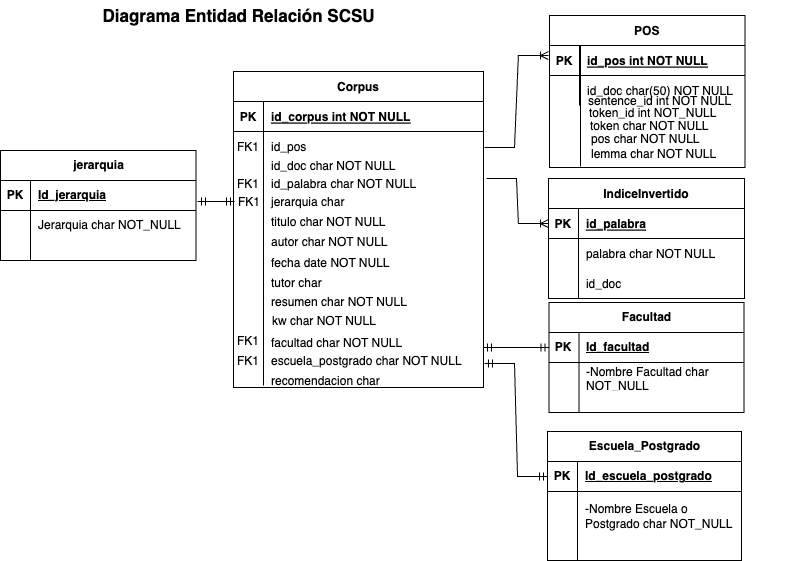
\includegraphics[width=0.9\linewidth]{images/05-desarrollo/4_ciclo/diagrama_entidadrel_SCSU} 

}

\caption{SCSU: Diagrama Entidad Relación}\label{fig:diagramer}
\end{figure}

Adicionalmente a la tabla ``Corpus'' se le añade una columna que se corresponde con las ``recomendaciones'' generadas para cada documento, donde se almacena una \emph{string} que corresponde a una estructura de datos ``html''.

\hypertarget{diagrama-general-del-sistema--versiuxf3n-contenedores}{%
\subparagraph{Diagrama General del Sistema- versión contenedores:}\label{diagrama-general-del-sistema--versiuxf3n-contenedores}}

En la figura \ref{fig:diagramacontenedores} se define la estructura que será implementada, teniendo en cuenta los Requerimientos Funcionales y No Funcionales indicados anteriormente. La propuesta funciona como un Sistema Distribuido, ver \ref{SD}, donde mediante el uso de contenedores, ver \ref{contenedores}, se crean instancias en las que son ejecutadas los servicios necesarios para que el Sistema Complementario Saber UCV puede cumplir con los objetivos propuestos. La integración y la asignación de recursos a cada contenedor se hace mediante el uso de un orquetador, ver \ref{orquestador}.

\begin{figure}

{\centering 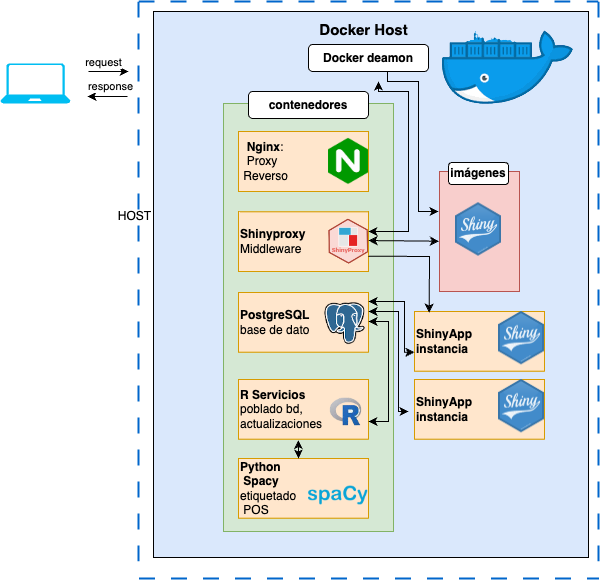
\includegraphics[width=0.8\linewidth]{images/05-desarrollo/4_ciclo/digrama_contenedores_modulos} 

}

\caption{SCSU: Diagrama General del Sistema en Contenedores}\label{fig:diagramacontenedores}
\end{figure}

En la fase de colaboración de este ciclo \ref{implemencolab} se especificarán las tareas y funciones asignadas a cada contenedor.

\hypertarget{esquema-general-de-clasificaciuxf3n-y-extracciuxf3n-de-datos-del-scsu}{%
\subparagraph{Esquema General de Clasificación y Extracción de Datos del SCSU:}\label{esquema-general-de-clasificaciuxf3n-y-extracciuxf3n-de-datos-del-scsu}}

En la figura \ref{fig:diagramaextra} se observa el proceso de extracción y clasificación de datos que realizará el SCSU, obteniendo los valores desde el repositorio Saber UCV, teniendo dos ramas principales que alimentan a la base de datos.

La lógica de este proceso es que en la primera rama se descarga el documento anexo a cada investigación, cuando se cumplan las condiciones, se hace la lectura del documento y se inicia el proceso de clasificación por facultad y área de estudio, como se vio en la ``Iteración- Extracción y Clasificación de las Investigaciones'' en \ref{asignacion}.

En la segunda rama se hace el ``etiquetado del discurso'', que fue revisado en la ``Iteración- Preparación del Corpus'' en \ref{iternlp}.

Ambos procesos alimentarán a las correspondientes tablas en la Base de Datos.

El proceso indicado se ejecuta inicialmente para realizar el poblado de la Base de Datos e igualmente se replica periódicamente, según parámetro definido en el archivo de configuración del orquestador, para actualizar e incorporar las nuevas investigaciones que se encuentren disponibles en el repositorio Saber UCV.

\begin{figure}

{\centering 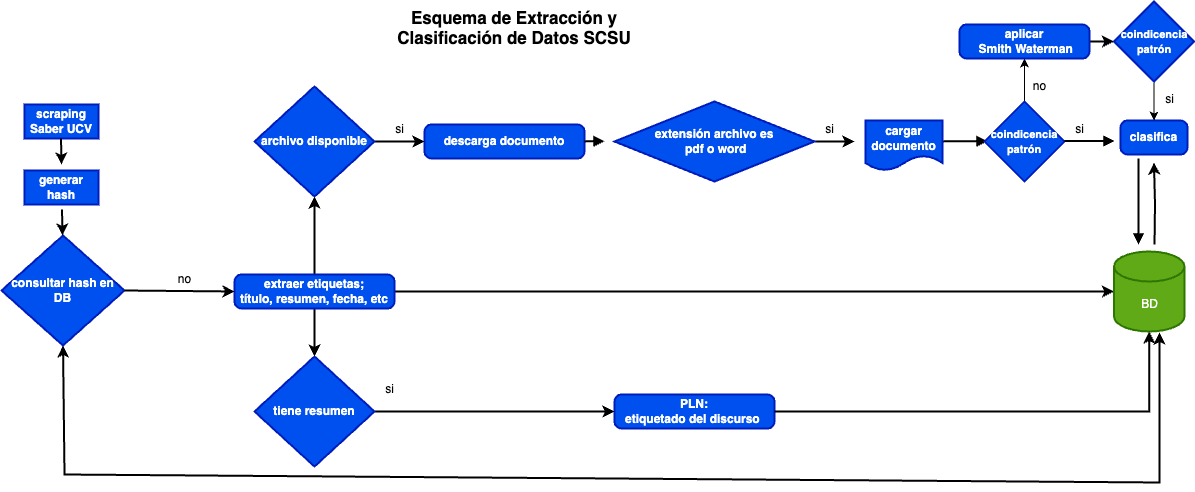
\includegraphics[width=0.9\linewidth]{images/05-desarrollo/4_ciclo/esquema extraccion} 

}

\caption{Esquema Extracción y Clasificación de Datos}\label{fig:diagramaextra}
\end{figure}

\hypertarget{interfaz-visual-mock-up}{%
\subparagraph{Interfaz Visual (Mock Up):}\label{interfaz-visual-mock-up}}

La interfaz cuenta con tres componentes:

\begin{enumerate}
\def\labelenumi{\arabic{enumi}.}
\item
  \textbf{Sidebar:} en la barra lateral que se ubicará en la parte izquierda de la aplicación y es el área donde el usuario definirá el texto de búsqueda así como los paremetros que le acompañan. En la figura \ref{fig:sidebar2} se puede ver el diseño propuesto.

  \begin{figure}

  {\centering 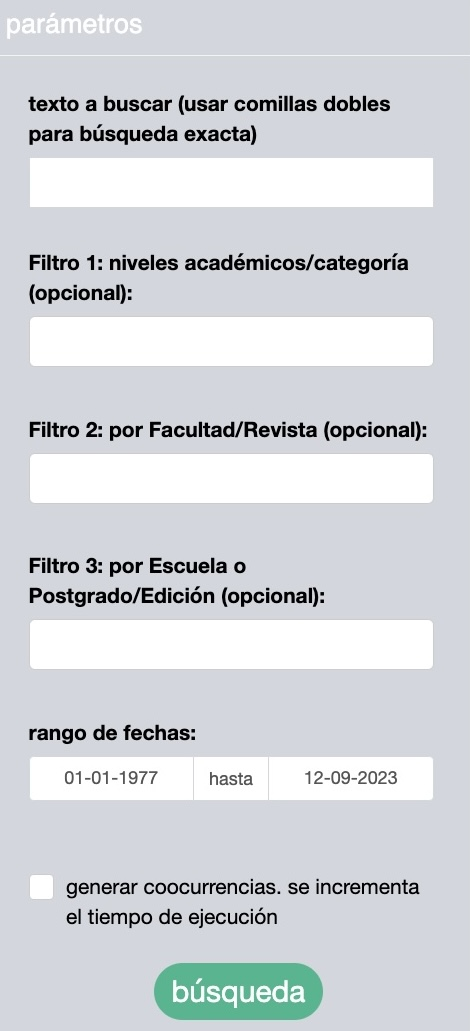
\includegraphics[width=0.2\linewidth]{images/05-desarrollo/4_ciclo/UI/sidebar} 

  }

  \caption{Interfaz de Usuario - Sidebar}\label{fig:sidebar2}
  \end{figure}
\item
  \textbf{Main Tabs:} es la sección de pestañas que se encontrará en la parte media alta de la aplicación y es donde el usuario podrá seleccionar la visualización de los ``tabla resultados'', bien sea para los tabla de los textos o para ver los ``mapas del conocimiento''. En la figura \ref{fig:maintab} se representa la propuesta. Al seleccionar una pestaña está cambiará el color de fondo verde a gris.

  \begin{figure}

  {\centering 
\includegraphics[width=0.9\linewidth]{images/05-desarrollo/4_ciclo/UI/maintab} 

  }

  \caption{Interfaz de Usuario - Pestañas }\label{fig:maintab}
  \end{figure}
\item
  \textbf{Resultados:} debajo de ``Main Tabs'' se presentan los resultados obtenidos en el proceso de búsqueda. La representación es contextual basada en la selección de pestaña que está seleccionada (``tabla resultados'' o ``mapas de conocimiento'').

  \begin{enumerate}
  \def\labelenumii{\arabic{enumii}.}
  \item
    En las figura \ref{fig:tablaresultados2} se puede ver la representación de la tabla de resultados de una búsqueda.

    \begin{figure}

    {\centering 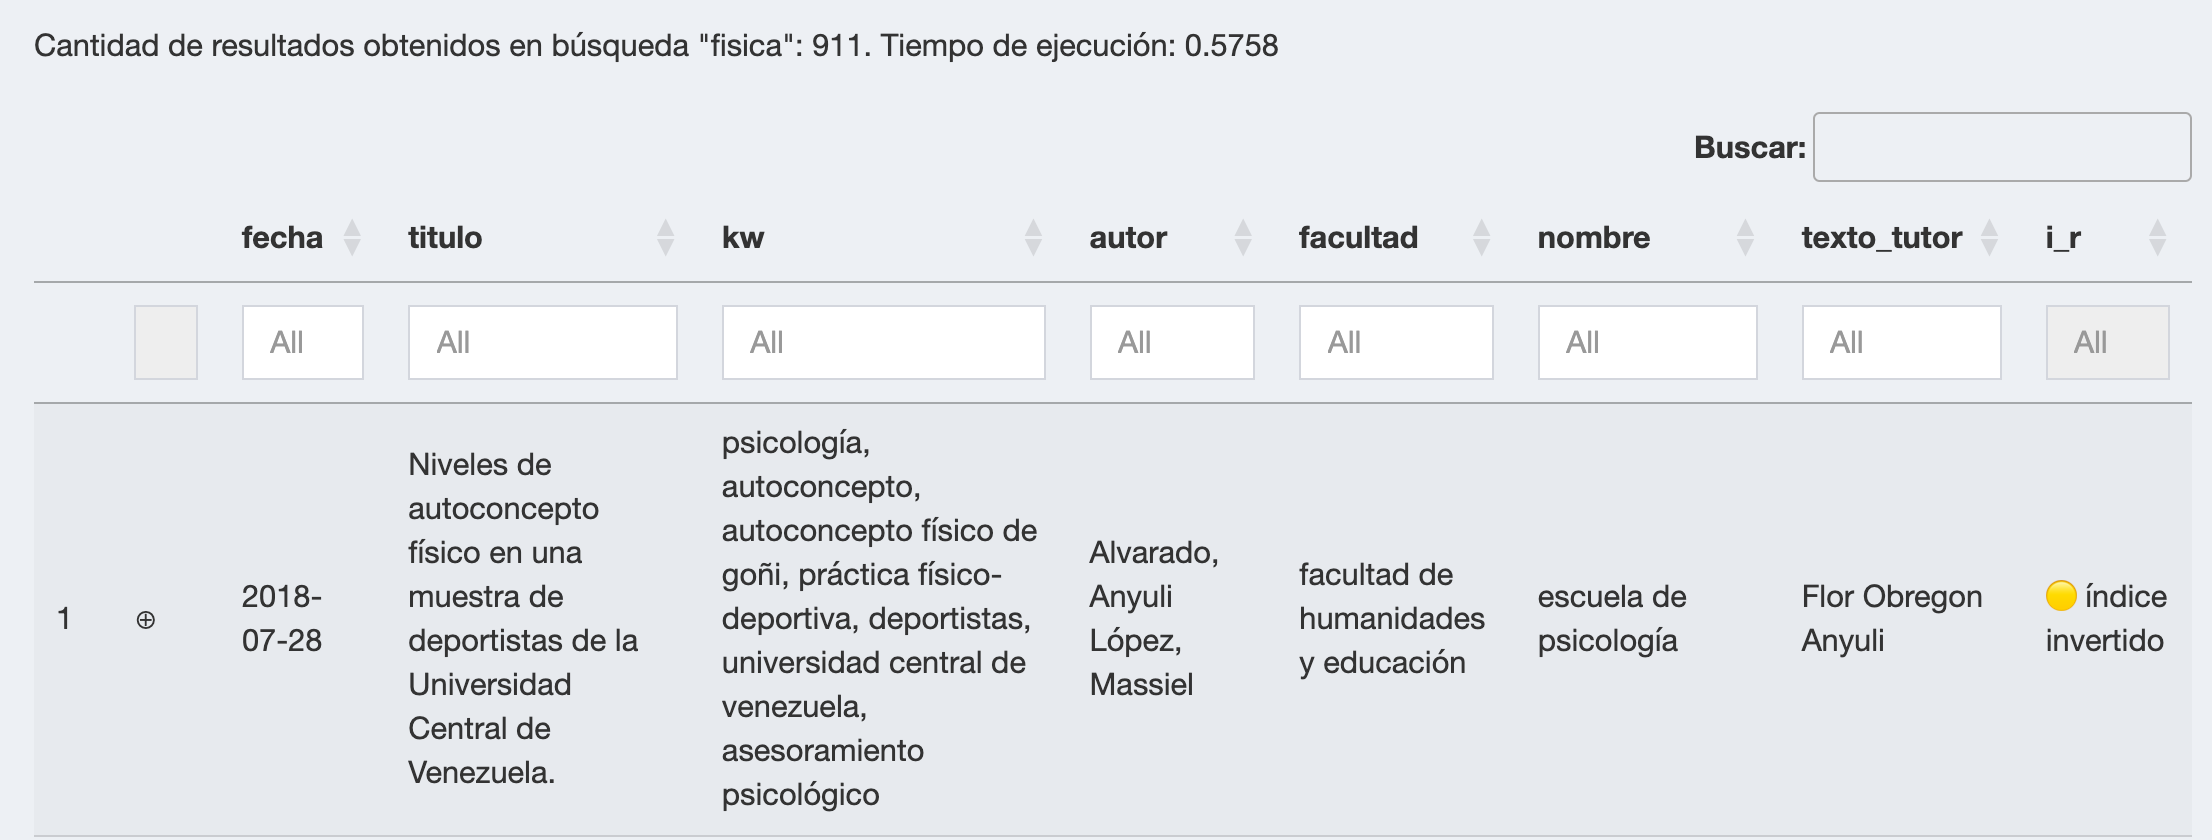
\includegraphics[width=0.9\linewidth]{images/05-desarrollo/4_ciclo/UI/tablaresultado} 

    }

    \caption{Interfaz de Usuario - Tabla Resultados de Búsqueda}\label{fig:tablaresultados2}
    \end{figure}
  \item
    En las figura \ref{fig:tablaresultados3} se puede ver la representación propuesta de ``mapas de conocimiento''.

    \begin{figure}

    {\centering 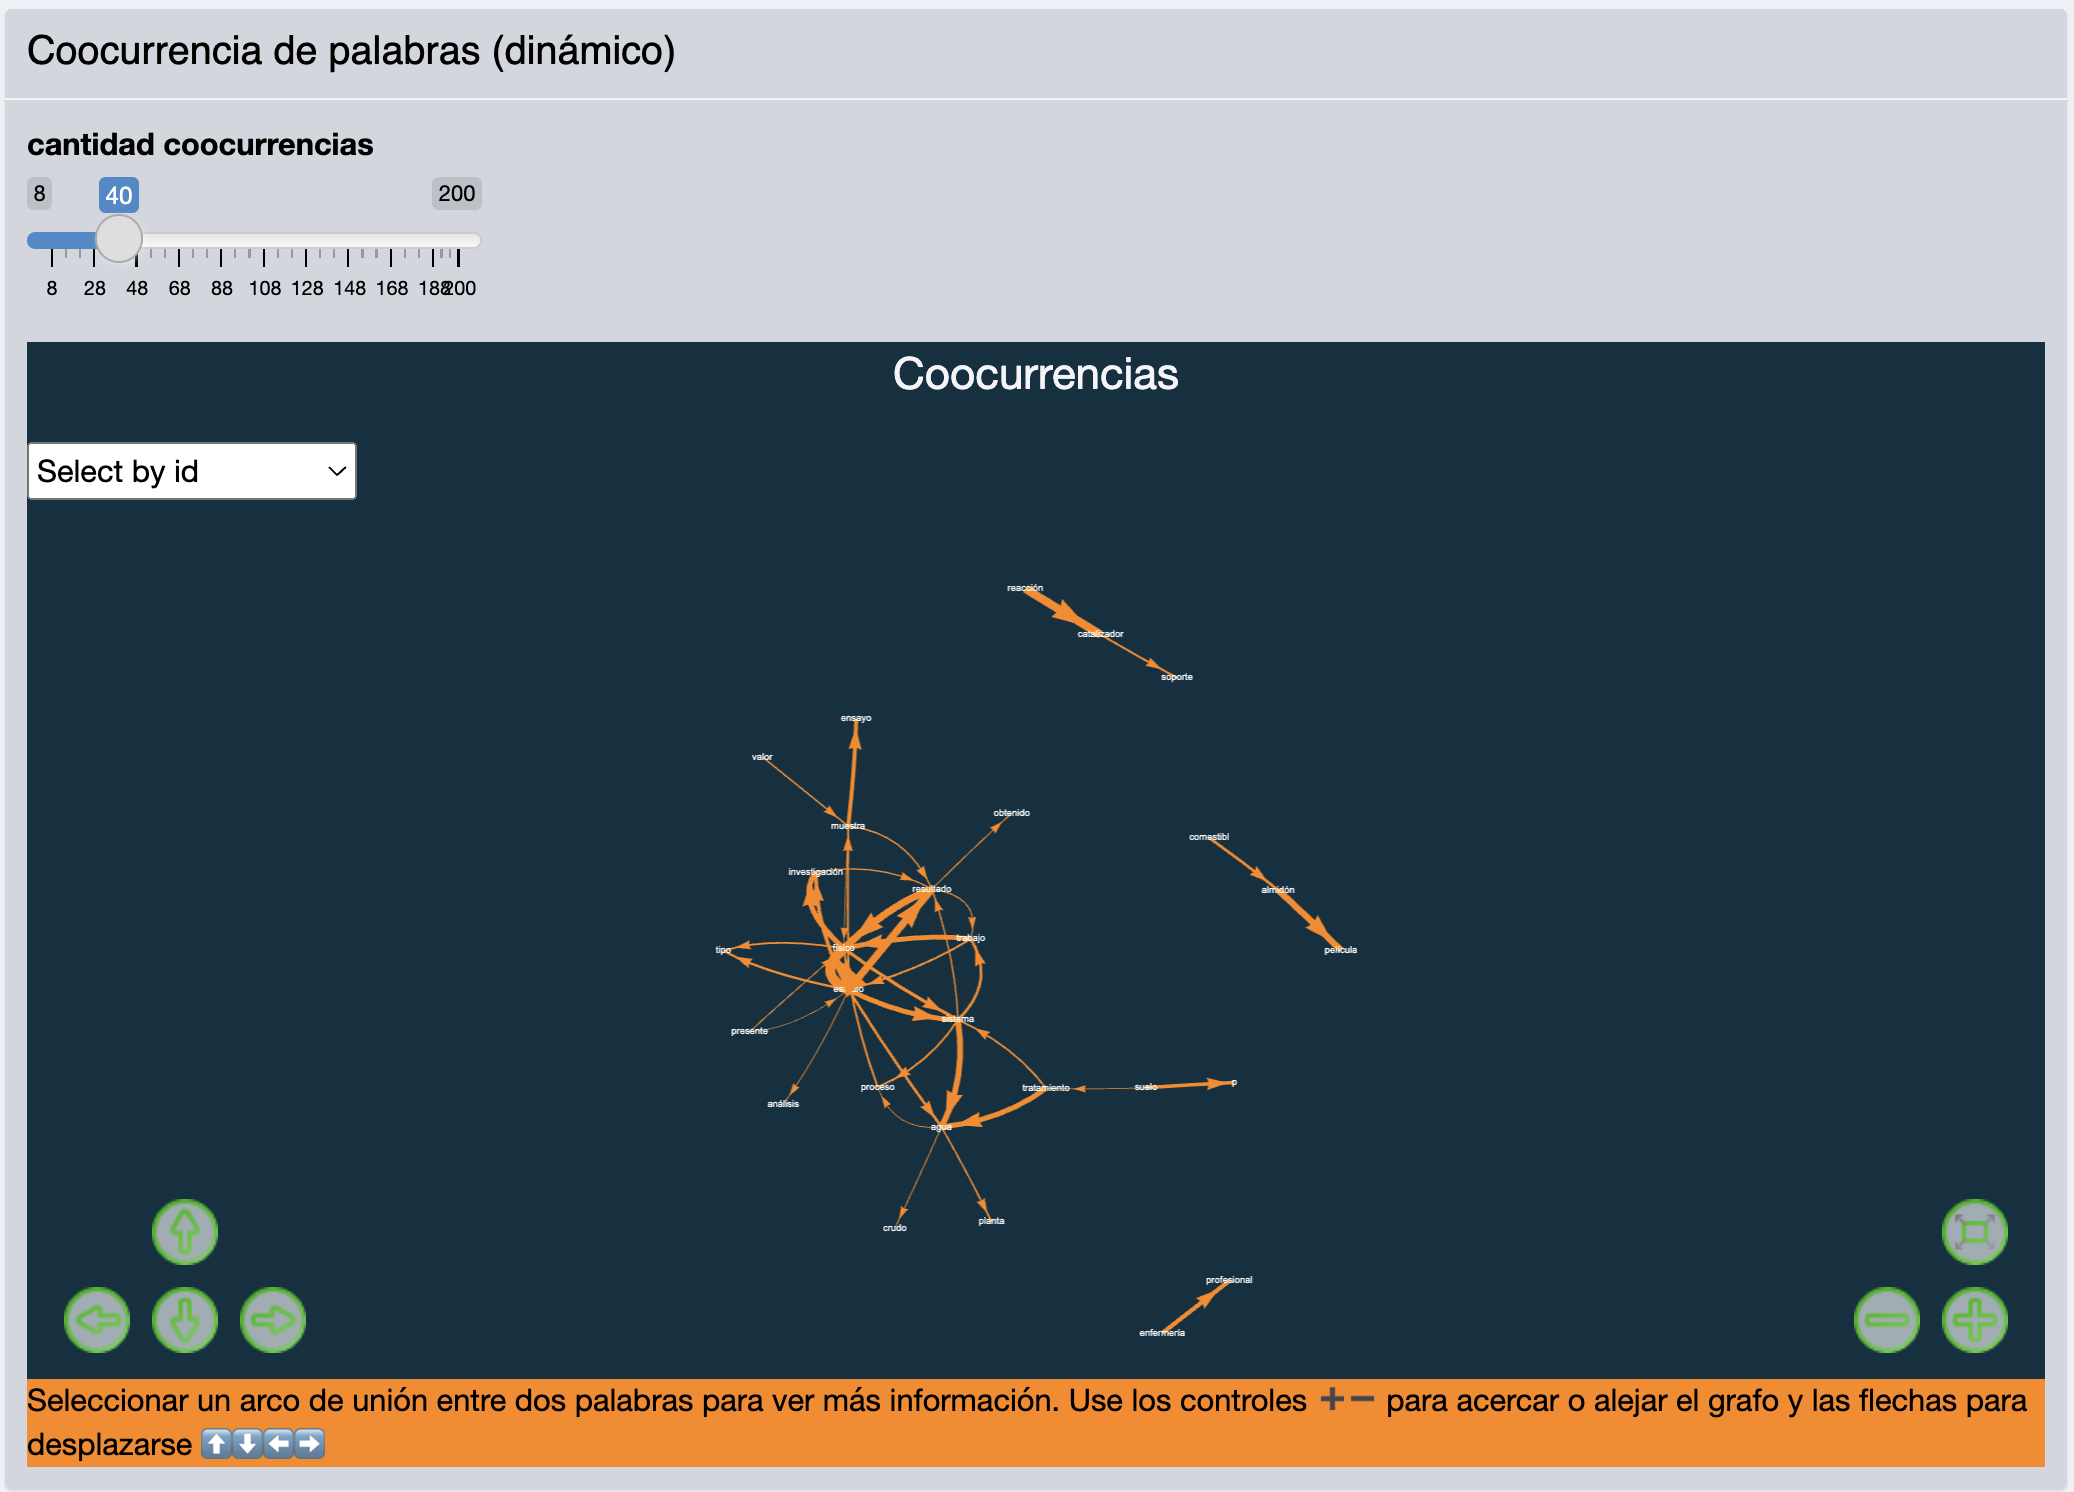
\includegraphics[width=0.7\linewidth]{images/05-desarrollo/4_ciclo/UI/uimapas} 

    }

    \caption{Interfaz de Usuario - Mapas de Conocimiento}\label{fig:tablaresultados3}
    \end{figure}
  \end{enumerate}
\end{enumerate}

Adicional a estos tres componentes la propuesta de intefaz incluye:

\begin{enumerate}
\def\labelenumi{\arabic{enumi}.}
\item
  \textbf{Tooltips}: al hacer hoover por áreas de introducción o selección de valores se despliegará un texto de ayuda según se ve en la \ref{fig:tooltip}.

  \begin{figure}

  {\centering 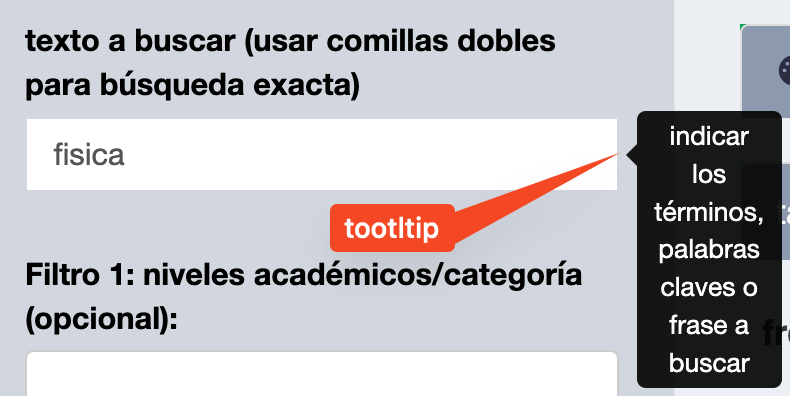
\includegraphics[width=0.3\linewidth]{images/05-desarrollo/4_ciclo/UI/tooltip} 

  }

  \caption{Interfaz de Usuario - Tooltips }\label{fig:tooltip}
  \end{figure}
\item
  \textbf{Inspección documento:} la tabla de resultados dispondrá de un ícono ``+'' que expande la tabla para mostrar el detalle y recomendaciones de un documento, como se observa en la figura \ref{fig:detalledoc}.

  \begin{figure}

  {\centering 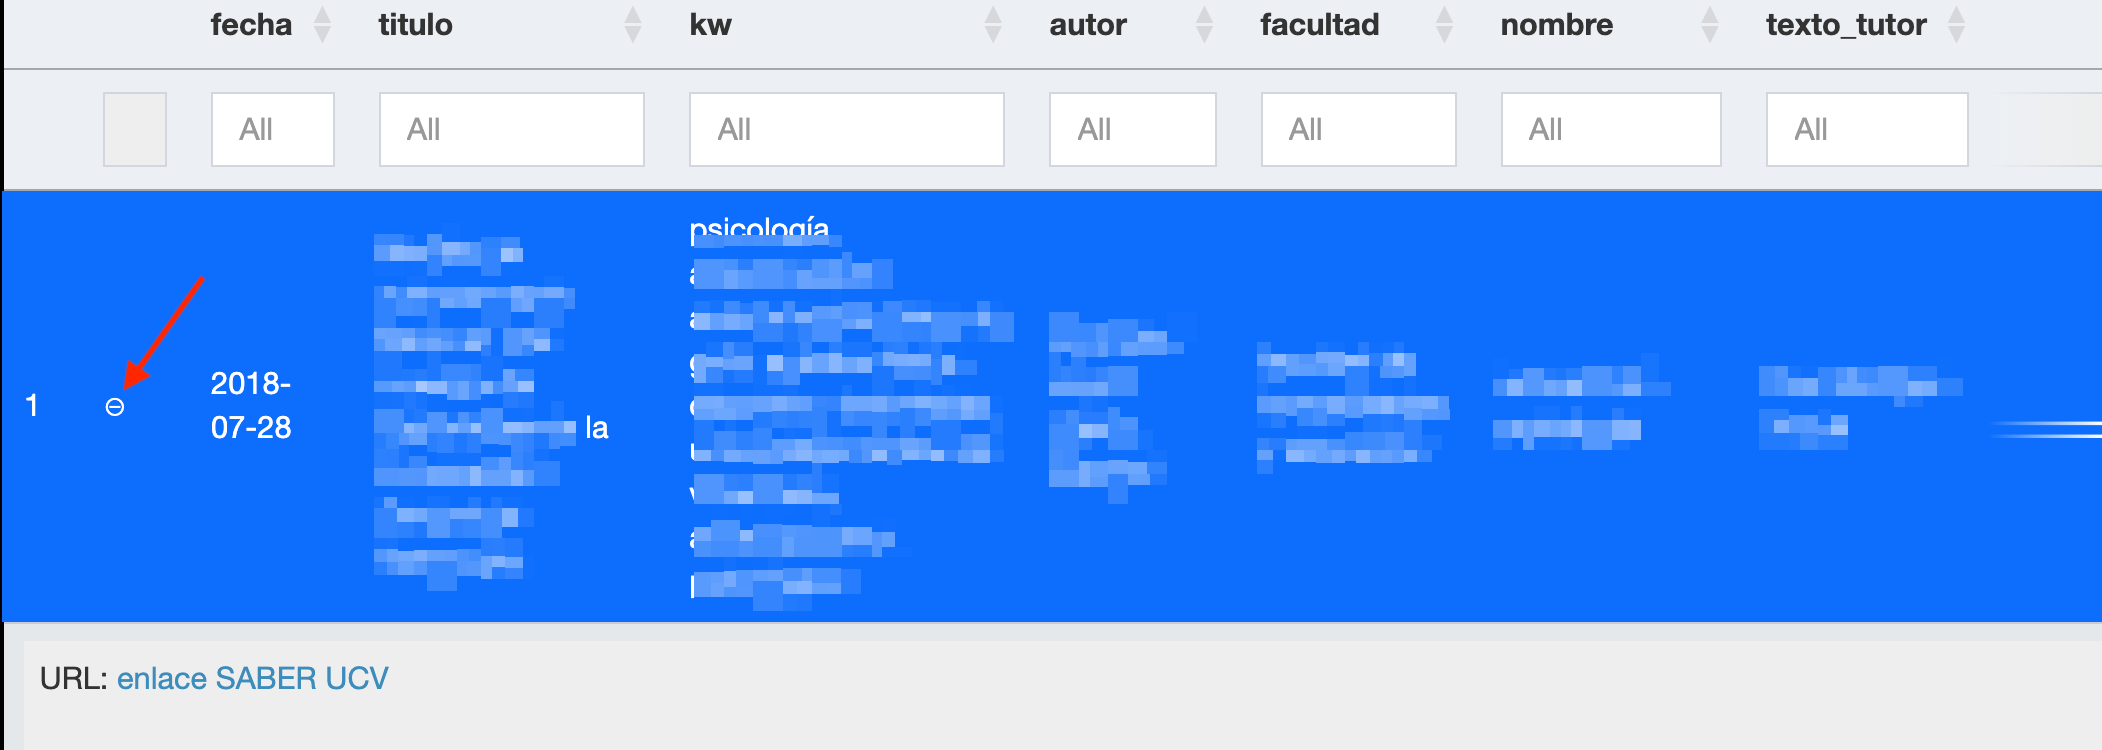
\includegraphics[width=0.8\linewidth]{images/05-desarrollo/4_ciclo/UI/uiinspecciontabla} 

  }

  \caption{Interfaz de Usuario -Inspección Documento }\label{fig:detalledoc}
  \end{figure}
\item
  \textbf{Inspección ``mapas de conocimiento'':} la propuesta de visualización del detalle de aparición en documentos de una determinada coocurrencia de dos palabrasque se encuentran unidas por un arco se ven en la figura \ref{fig:detallemc}. La tabla que se muesta aparecerá mediante una ventana desplegable.

  \begin{figure}

  {\centering 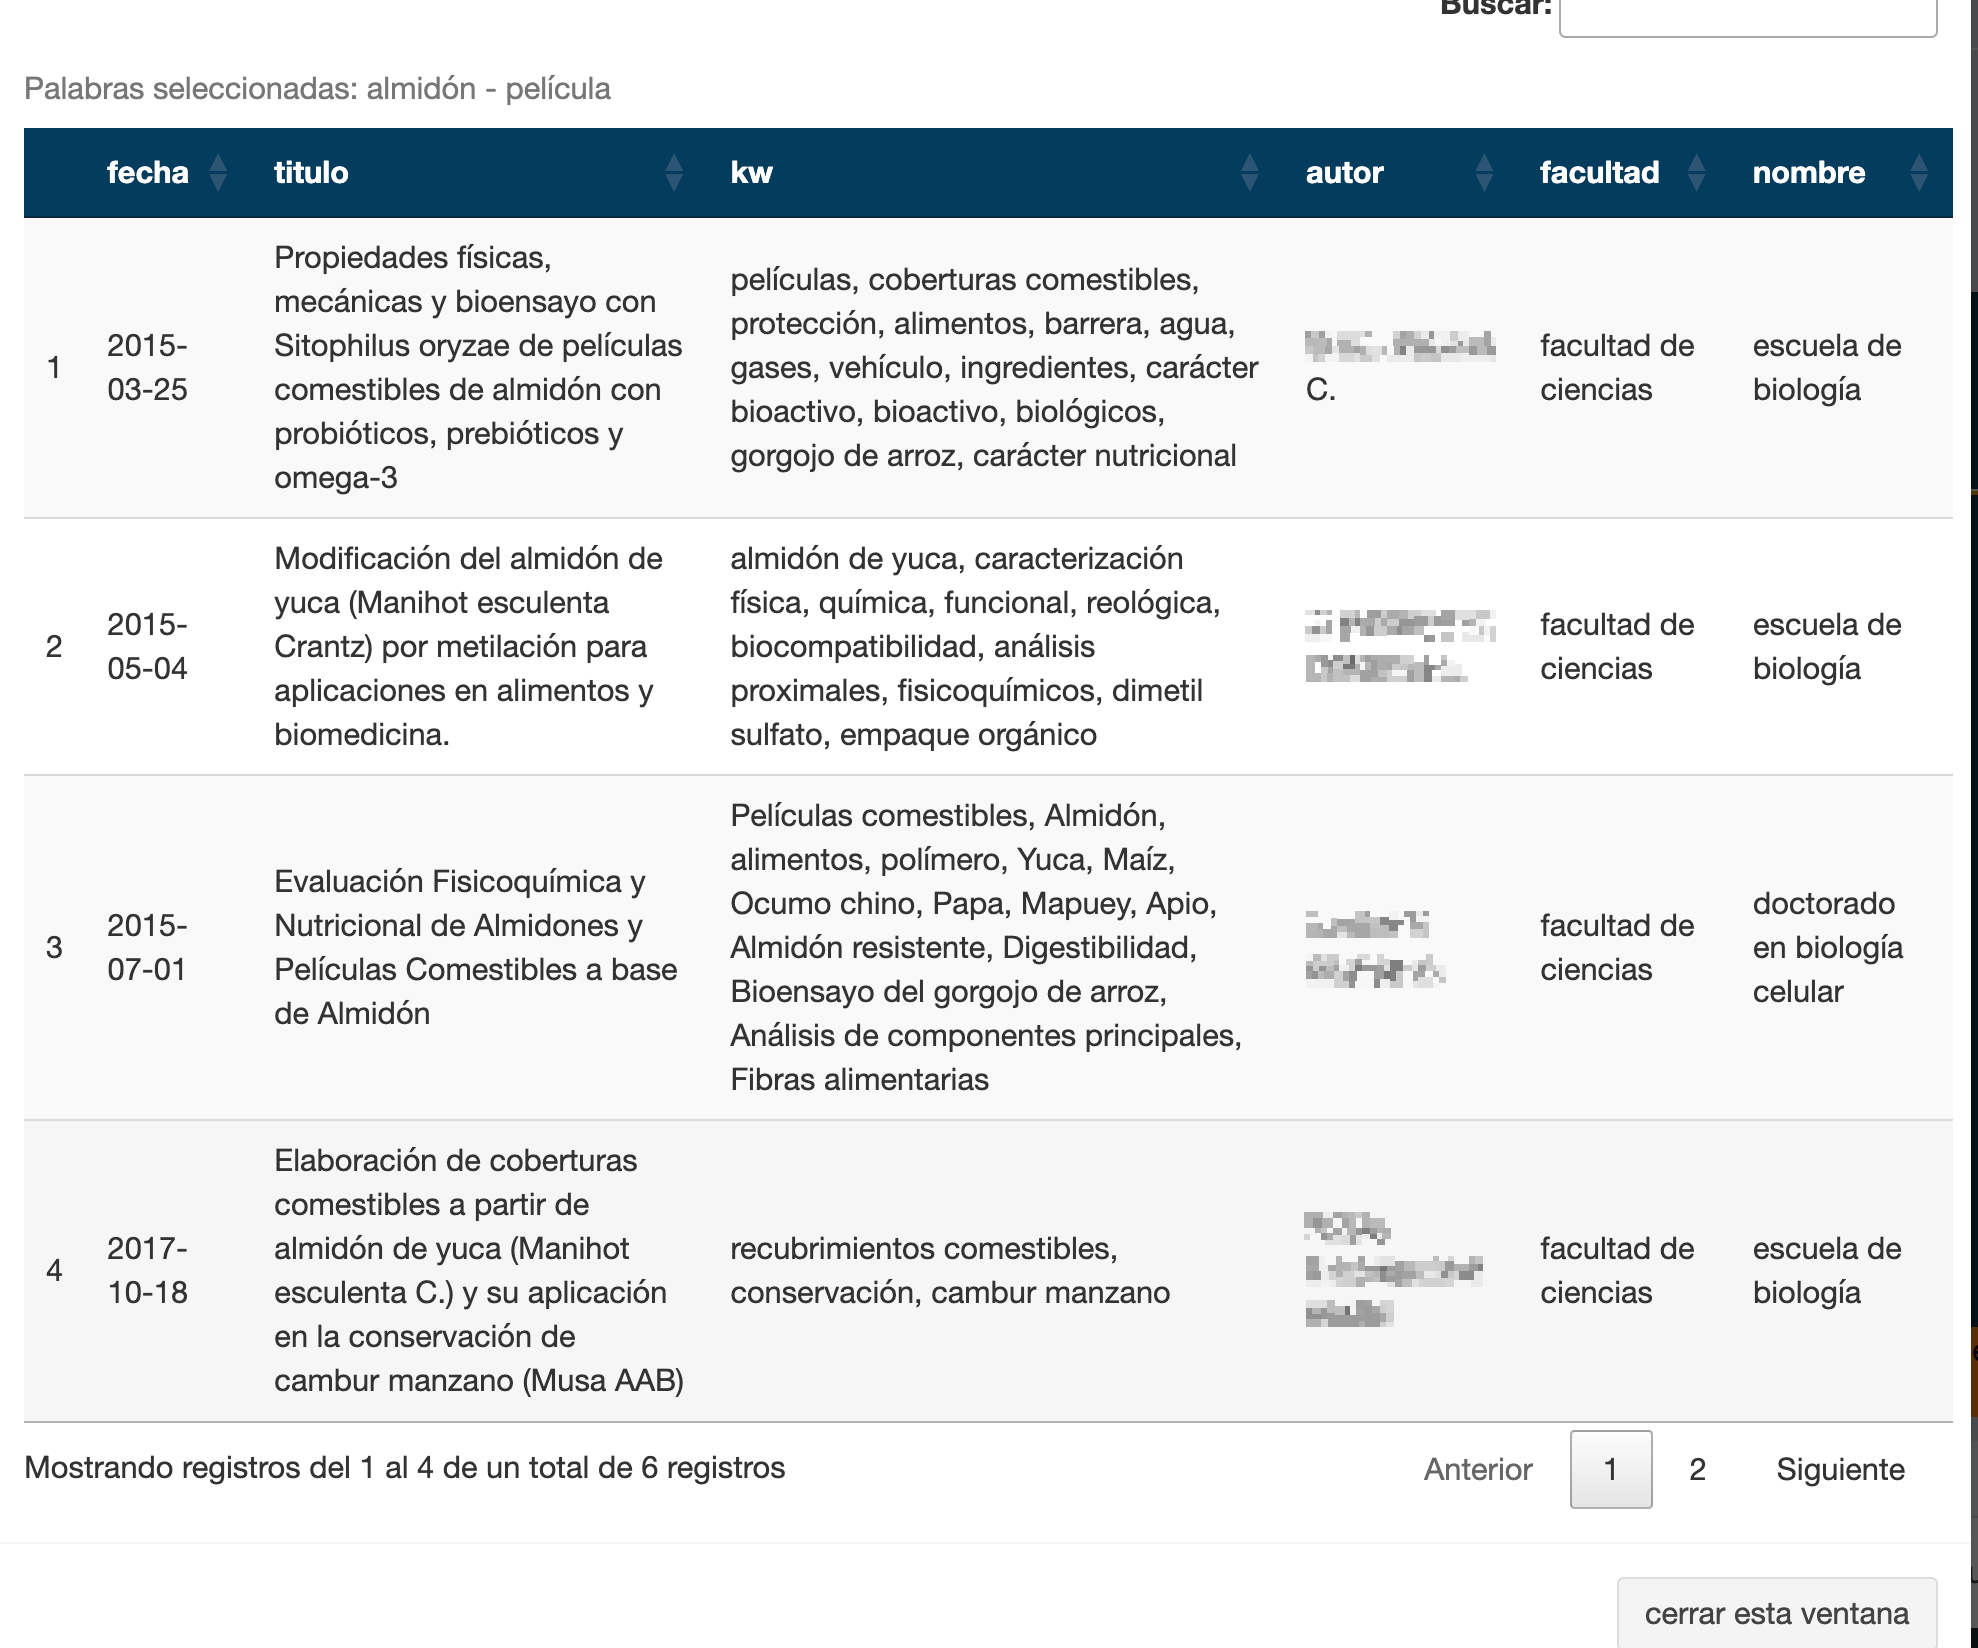
\includegraphics[width=0.6\linewidth]{images/05-desarrollo/4_ciclo/UI/uiinspeccionmapas} 

  }

  \caption{Interfaz de Usuario- Inspección Mapas de Conocimiento }\label{fig:detallemc}
  \end{figure}
\end{enumerate}

\hypertarget{muxf3dulos-aplicaciuxf3n-web}{%
\subparagraph{Módulos Aplicación Web:}\label{muxf3dulos-aplicaciuxf3n-web}}

La aplicación web, que será desarrollada en el \emph{framework} ``Shiny'', según las prácticas de desarrollo recomendadas, se hace bajo la arquitectura de módulos denominados ``Shiny Modules'', descomponiendo en partes independientes cada par de funciones relacionadas en la \emph{UI} (define la interfaz de usuario) y el \emph{Server} (define la lógica del servidor), facilitando la comprensión del funcionamiento de la aplicación, la legibilidad del código, pruebas unitarias y el mantenimiento \citep{wickham2021}. En la figura \ref{fig:shinymodulo} se puede ver la arquitectura de la aplicación que se integrará dentro del Sistema distribuido.

\begin{figure}

{\centering \includegraphics[width=0.6\linewidth]{images/05-desarrollo/4_ciclo/digrama_shinyapp_modulos} 

}

\caption{Diagrama Aplicación Web Shiny Versión Modular}\label{fig:shinymodulo}
\end{figure}

\hypertarget{implemencolab}{%
\paragraph{Colaboración:}\label{implemencolab}}

Según lo propuesto en la fase de Especulación \ref{implemenesp} se hizo el desarrollo del Sistema mediante un conjunto de contenedores orquestados, tomando en consideración que es necesario implementar los mecanismos de comunicación necesarios con la definición de una red y de disponer de un volumen compartido con la máquina host.

En la implementación se usaron ampliamente los conocimientos adquiridos en ciclos anteriores, no obstante también se tuvieron que revisar documentaciones, probar distintas opciones de librerías e imágenes de contenedores que permitiesen llevar a un entorno de producción, con la debida integración de los componentes, el Sistema planificado.

\hypertarget{contenedores-1}{%
\subparagraph{Contenedores:}\label{contenedores-1}}

Para realizar la implementación del Sistema, apoyado en contenedores para los distintos servicios que lo conforman, se eligió docker como herramienta. Mediante un archivo denominado ``dockerfile'' para cada servicio se especificó el entorno, dependencias y configuraciones necesarias para crear la imagen que servirá para instanciar cada contenedor.

A continuación se indican los contenedores que forman parte del Sistema y los puertos que disponden para interactuar unos con otros:

\begin{enumerate}
\def\labelenumi{\arabic{enumi}.}
\item
  \textbf{Nginx:} Es el servidor web/proxy inverso de código abierto que en este Sistema se usa para redireccionar las peticiones del cliente recibidas en el puerto 80 y 443 al puerto 8080. En este contenedor también se almacena el certificado SSL para permitir conexiones por el protocolo HTTPS en caso de configurar un dominio\footnote{Al momento de presentar este Trabajo de Grado no se dispone de un dominio para realizar la configuración del certificado para conexiones HTTPS, no obstante en un momento previo en que se tenía disponible un dominio se hicieron las pruebas para comprobar la integración y correcto funcionamiento.}. Este contenedor fue generado desde una imagen oficial de NGINX que se encuentra en el ``docker hub'' sin añadir ninguna capa (layer) adicional.
\item
  \textbf{Cerbot:} es una herramienta de código abierto que permite tramitar y habilitar las conexiones mediante el protocolo HTTPS con el uso de un certificado ``Let´s Encrypt''. El uso de este certificado está asociado al uso de un dominio en el \emph{deploy} de la aplicación. Este contenedor fue generado desde una imagen de CERBOT del ``docker hub'' sin realizar ninguna modificación.
\item
  \textbf{Shinyproxy:} es una solución de código abierto para alojar aplicaciones Shiny \citep{shinyproxy2023} que cuenta con una tecnología estable y probada. El uso de este contenedor se justifica en el hecho de que una aplicación Shiny funciona como ``single thread'' y es necesario que ante cada petición de acceso, al servidor despliegue un \emph{workspace} completamente aislado, es decir, un contenedor distinto. Shinyproxy es una implementación del servidor ``\emph{Spring boo}t'' que tiene la capacidad de hacer la replicación indicada y permite controlar los recursos de memoria y cpu asignados, así como el timeout a cada instancia que se despliega. Otras ventajas que aporta, no implementadas en esta versión del Sistema, es que permite establecer \emph{login} en el uso de la aplicación y la creación de grupos de usuarios con perfiles distintos, contando con soporte para distintos métodos de autenticación. Si bien en estos momentos la aplicación está concebida para el libre acceso, en algún momento se pude restringir y no sería necesario hacer modificaciones en la arquitectura, más allá de variaciones en el archivo de configuración. Este contenedor habilita el puerto 8080 para escuchar las peticiones y fue generado desde la imagen del docker hub \emph{Shinyproxy}.
\item
  \textbf{``\emph{Shiny Web App}''}: En este contenedor se encruentra la imagen de la aplicación web con todas las dependencias y librerías necesarias para remitir los \emph{querys} al contenedor del manejador de la base de datos, presentar los resultados y generar las visualizaciones correspondientes. Como se indicó anteriormente, cada vez que ocurre desde el navegador del cliente una petición de acceso, desde el contenedor \emph{shinyproxy} , se crea una instacia de este contenedor con todos los elementos necesarios para que la app funcione. En caso de presentar alguna falla, el sistema es tolerante a los mismos, porque se pueden seguir recibiendo peticiones que replicarían una imagen nueva del contenedor sin afectar al que presentase el fallo, o viceversa. Desde este contenedor se realiza el acceso de lectura al contenedor que contiene \emph{PostgreSQL} donde reposa la base de datos que contiene los textos ya procesados. La imagen que se usa en este servidor fue definida a medida.

  Parte de las configuraciones de la interfaz de usuario se realizan en un archivo \emph{css} para facilitar modificaciones que puedan resultar de interés.

  \textbf{Lógica de la aplicación:}

  El esquema general de la aplicación es similar al que se presentó en el Prototipo en la figura \ref{fig:esqshinyproto}. A continuación se mencionan las entradas y salidas que se generan dentro del contenedor.

  \begin{enumerate}
  \def\labelenumii{\arabic{enumii}.}
  \item
    \textbf{Entradas:}

    \begin{enumerate}
    \def\labelenumiii{\arabic{enumiii}.}
    \item
      \textbf{Defición query:} Contiene un campo para la entrada de texto con el que se generará el query.- Contiene un selector para indicar si se quiere generar la coocurrencia de palabras- Contiene tablas para seleccionar: 1) Nivel académico del trabajo. Opciones (pregrado, especialización, maestría, doctorado). 2) Facultad o Centro de adscripción. Opciones: 11 Facultades más un centro (CENDES). 3) Nombre del pregrado o postgrado. En total son 412 las opciones. Cada una de las tablas anteriores se actualiza según se vayan seleccionando las relaciones y la disponibilidades. Por ejemplo, al seleccionar pregrado solo se mostrarán los nombres de las carreras de pregrado, pero si se selecciona también el nombre de la Facultad, sólo se mostrarán las carreras de pregrado dentro de la Facultad seleccionada. Para una determinado filtro se permiten selecciones múltiples dando una total flexibilidad al momento de ejecutar los \emph{querys}. El texto del \emph{query} es procesado convirtiéndolo a minúsculas y removiendo signos de puntuación.
    \item
      \textbf{Selector ``generar coocurrencias'':} es una casilla que sirve para seleccionar si se van a representar los Mapas de Conocimiento o no. Por defecto está desselccionado ya que la representación de los mapas incrementa el tiempo de procesamiento de los datos.
    \item
      \textbf{``Clic'' inspeccionar documento:} al obtener los resultados en una tabla se puede inspeccionar un documento particular para ver el texto resumen y las recomendaciones de documentos similares.
    \item
      \textbf{Cantidad de coocurrencias:} teniendo como condición que previamente se seleccionara ``generar coocurrencias'',dentro de la pestaña de ``Coocurrencias'', correspondientes a los Mapas de Conocimiento, se puede modificar la cantidad de coocurrencias a representar. El valor por defecto representado es 60.
    \item
      \textbf{``Clic'' inspeccionar Mapa de Conocimiento:} dentro de la pestaña de ``Coocurrencias'', correspondientes a los Mapas de Conocimiento, al tener representadas dos palabras mediante nodos, existe un arco que las une. Sobre el arco se puede hacer clic e inspeccionar los documentos que contienen las palabras asociadas por el arco.
    \end{enumerate}
  \item
    \textbf{Salidas:} Ante el \emph{query} se genera:

    \begin{enumerate}
    \def\labelenumiii{\arabic{enumiii}.}
    \item
      \textbf{Resultados query:} en una tabla creada con la librería ``DT'' se muestra el listado de documentos recuperados mostrando en cada fila los siguientes atributos: autor, fecha, palabras clave, texto resumen, nombre tutor. Los documentos a presentar y el orden en que son presentados viene desde el contenedor ``PostgreSQL''. Adicionalmente se muestra un enlace al repositorio Saber UCV donde se encuentra alojado el respectivo trabajo (el documento en PDF). Igualmente se presentan los textos que tienen mayor similitud con el documento seleccionado. Un gráfico con la frecuencia por año de los trabajos extraídos mediante el \emph{query}. El gráfico se generá con la librería ``apexcharter'', por lo cual tiene ciertas interactividades mostrando con el \emph{hoover} el valor de la cantidad por año que está representada en cada columna.
    \item
      \textbf{Mapas de Conocimiento dinámico:} Gráfico de coocurrencia interactivo de palabras que se genera mediante la librería de ``VisNetwork\emph{''} . Este gráfico permite distintas interacciones con el usuario como hacer zoom (in-out), seleccionar un determinado nodo, usar las teclas izquierda, derecha, arriba y abajo del teclado, así como también permite seleccionar un arco de unión entre dos palabras coocurrentes. Al realizar la selección se filtran un subconjunto de los documentos que contienen ambas palabras representadas por nodos. Los documentos filtrados se mostrarán en una tabla contigua, también generada en''DT'', donde sólo se incluye el texto resumen de cada trabajo.
    \item
      \textbf{Mapas de Conocimiento Estático:} gráfico de coocurrencias estático de palabras, donde mediante la librería ``ggraph\emph{''} son generados un par de gráficos con distintas granularidades. El primero exhibe la misma coocurrencia de palabras expuesta en el punto con una visualización estática. En cuanto a la granularidad se muestran las palabras que coocurren dentro de todo el resumen independientemente de la proximidad que tengan. El segundo gráfico también muestra la coocurrencia, pero solo de palabras que se encuentran en el texto resumen una seguida de otra representando los resultados con una menor granularidad.Con la librería''UdPipe\emph{``} se generan las estructuras de datos necesarias para generar los grafos (arcos y nodos).

      En el Apéndice \ref{apendicea} se listan los paquetes que usa este contenedor.
    \end{enumerate}
  \end{enumerate}
\item
  \textbf{``PostgreSQL'':} es el contenedor donde se encuentra el manejador de PostgreSQL versión 16 y en él se almacenan todas las tablas que usa el Sistema. También recae la funcionalidad de generar el ``\texttt{ts\_vector}'', convertir el query a un ``\texttt{ts\_query}'' y mediante la función ``\texttt{ts\_rank}'' reordenar los resultados extraídos con base en un ranking junto con el indexado de las distintas tablas. En el ciclo ``Iteración- Implementación Prototipo'' \ref{desarrollociclos3} se indican más detalles sobre las funciones señaladas. En este contenedor se tiene una imagen de \emph{PostgreSQL} versión 16.1 extraída del ``docker hub'' a la cual no le fue realizada ninguna modificación distinta a la configuración para la definición de usuarios y contraseña junto con la definición de un volumen compartido con el \emph{host} para garantizar que se tengan ``datos persistentes''. Este contenedor recibe consultas del contenedor \textbf{``\emph{S}}\emph{hiny Web App}'' y escritura-lectura desde el contenedor ``R imagen Servicios'' teniendo habilitado el puerto 5432.
\item
  \textbf{``R Imagen Servicios''}: En este contenedor se creó una imagen con todos los servicios necesarios para realizar el \emph{web crawling}, el procesamientos de textos y la descarga de los archivos desde Saber UCV para realizar la clasificación de las Tesis y demás trabajos. Al iniciar la configuración del Sistema, contiene las funcionalidades que permiten realizar la creación de la base de datos, las tablas y el poblado de estas. Periódicamente es invocado un script mediante un ``cron job'' para realizar los procesos de incorporación de aquellos documentos nuevos que se detecte que están disponibles en Saber UCV. La imagen base que se usa es la del proyecto Rocker \citep{RJ-2017-065:2017}, la cual es una versión ampliamente probada y optimizada por la comunidad de usuarios de R.

  \textbf{Procesos:}

  \begin{enumerate}
  \def\labelenumii{\arabic{enumii}.}
  \tightlist
  \item
    \textbf{Poblado base de datos:} se ejecutan los procesos para hacer el poblado inicial de base de dato así como a la creación del indexado de la base de datos en el contenedor ``\textbf{PostgreSQL''.} En la fase de especulación de este ciclo se presentó un diagrama que describe el esquema de''extracción y clasificación de los datos'', ver figura \ref{fig:diagramaextra}.
  \item
    \textbf{Descarga de datos:} proceso que fue abordado en el ``Ciclo Conformación del Conjunto de Datos''.
  \item
    \textbf{Text Mining y NLP:} en el ``Ciclo Prototipo SCSU'', ver \ref{desarrollociclos3}, en la iteración ``Preparación del Corpus'', ver \ref{iternlp}, se detallan los procesamientos a los textos que ahora son ejecutados en este contenedor. La diferencia es que para usar ``spacyr'', al depender esta librería de una ambiente virtual en python , es necesario configurar otro contenedor con las dependencias y librerías que permitan el llamado al etiquetado del discurso. El contenedor que se integra para realizar estos procesos es \textbf{``Python Spacy''.}
  \item
    \textbf{Generación de recomendaciones:} se corresponde con detallado en el ``Ciclo Prototipo de SCSU'' en la iteración ``Recomendación de Documentos'', ver \ref{imrecomendacion}.
  \end{enumerate}

  En el Apéndice \ref{apendicea} se listan las librerías que usa este contenedor
\item
  \textbf{``Python Spacy'':} Se creó una imagen que contiene un ``Ubuntu 22'' con ``python 3.10'', la librería ``spacy v.3'' y el modelo de Spacy ``es\_core\_news\_lg'' . Su función es que mediante un volumen compartido pueda ser invocado desde el contenedor ``R Imagen Servicios'' para así realizar los procesamientos de NLP descritos.
\end{enumerate}

\hypertarget{orquestador-1}{%
\subparagraph{Orquestador:}\label{orquestador-1}}

Todos los contenedores mencionados es necesario que actúen de forma coordinada, compartiendo recursos como una red y volúmenes de almacenamiento. Para lograr esto se acude a la herramienta ``Docker Compose'' que se instala en el \emph{host} y permite simplificar y automatizar el despliegue de aplicaciones compuestas por múltiples servicios y contenedores en entornos de desarrollo y producción.

Se define la infraestructura, configuración y gestión de una aplicación a través de un archivo YAML, denominado ``docker-compose.yml'' donde se detallan los servicios, contenedores, redes y volúmenes necesarios para la aplicación, así como las relaciones y configuraciones entre ellos, simplificando la orquestación de los contenedores.

También la adopción de Docker Compose facilita la replicación del entorno de desarrollo en diferentes máquinas, mejorando la consistencia en el desarrollo.

La responsabilidad del administrador queda reflejada en la definición de distintas variables de entorno contenidas en el archivo docker compose, como lo es la definición del período de actualización de los textos.

\hypertarget{mantenimiento-del-scsu}{%
\subparagraph{Mantenimiento del SCSU:}\label{mantenimiento-del-scsu}}

De acuerdo a la implementación del Sistema, los procesos de mantenimiento que corresponde ejecutar al administrador, son los que se detallan a continuación:

\begin{enumerate}
\def\labelenumi{\arabic{enumi}.}
\item
  Respaldos regulares de la base de datos:

  \begin{itemize}
  \tightlist
  \item
    Se estableció un ``\emph{cron job}'' en el contenedor \textbf{``R Imagen Servicios''} para realizar respaldos automáticos de la base de datos PostgreSQL.
  \end{itemize}
\item
  Monitoreo del rendimiento:

  \begin{itemize}
  \tightlist
  \item
    Se utilizan herramientas de monitoreo para vigilar el rendimiento del contenedor PostgreSQL, Shinyproxy y Shiny.
  \end{itemize}
\item
  Logs y registro de eventos:

  \begin{itemize}
  \tightlist
  \item
    Registro de logs de contenedores en un volumen compartido con el \emph{host}.
  \end{itemize}
\item
  Gestión de dependencias:

  \begin{itemize}
  \tightlist
  \item
    Se documentan las dependencias específicas de la versión de PostgreSQL, Shinyproxy y Shiny.
  \end{itemize}
\item
  Seguridad de red:

  \begin{itemize}
  \tightlist
  \item
    Se configuró el \emph{firewall} y las reglas de red para limitar el acceso no autorizado a los contenedores.
  \end{itemize}
\item
  Escalabilidad:

  \begin{itemize}
  \tightlist
  \item
    Se realizaron pruebas de carga para identificar posibles cuellos de botella.
  \end{itemize}
\end{enumerate}

Eventualmente en caso del Sistema quedar en un entorno de Producción permanente, sería necesario agregar los siguientes procesos al Mantenimiento:

\begin{enumerate}
\def\labelenumi{\arabic{enumi}.}
\item
  Actualizaciones de seguridad:

  \begin{itemize}
  \tightlist
  \item
    Supervisar actualizaciones de seguridad para PostgreSQL y la imagen de Shiny.
  \end{itemize}
\item
  Control de versiones:

  \begin{itemize}
  \tightlist
  \item
    Utilizar un sistema de control de versiones para el código del SCSU.
  \end{itemize}
\item
  Documentación:

  \begin{itemize}
  \tightlist
  \item
    Mantener actualizada la documentación del sistema, incluyendo la configuración, dependencias y procedimientos de recuperación ante desastres.
  \end{itemize}
\end{enumerate}

\hypertarget{requerimientos-muxednimos-de-hardware}{%
\subparagraph{Requerimientos mínimos de hardware:}\label{requerimientos-muxednimos-de-hardware}}

Para un concurrencia de 4 usuarios simultáneos, estos son los requerimientos de hardware:

\begin{itemize}
\tightlist
\item
  2 CPU virtual
\item
  4 GB de memoria RAM
\item
  50 GB de disco duro
\end{itemize}

\hypertarget{implemenapre}{%
\paragraph{Aprender:}\label{implemenapre}}

Este Ciclo trajo un profundo y largo proceso de aprendizaje ya que el desarrollo implicó integrar distintos elementos abordados previamente de forma aislada, más el reto de encontrar componentes que fuesen compatibles y adaptados a los requerimientos funcionales y no funcionales planteados.

La utilidad de esta integración también representa en que se cuenta con un \emph{framework} que permite desplegar otro tipo de aplicaciones que pueden ser fácilmente escalables en entornos de producción o añadir módulos distintos al SCSU como pudiera ser una aplicación para la administración del sistema o consultar estadísticas de uso.

Como la cantidad de ciclos e iteraciones ejecutados previamente había sido extenso, en esta Ciclo, más allá del reto de la integración y evaluación de componentes, no fue de distinta índole el aprendizaje adquirido, sin embargo se decidió incorporar en la interfaz del usuario un gráfico que muestre la frecuencia de aparición de \emph{query} en el tiempo así como una representación estática de los ``mapas de conocimiento'' ya que en esta versión se presenta con una mejor perspectiva la coocurrencia de términos, a diferencia de la versión interactiva que está diseñada para inspeccionar en detalle una determinada aparición de términos.

\hypertarget{objetivos-alcanzados-2}{%
\subparagraph{Objetivos alcanzados:}\label{objetivos-alcanzados-2}}

\begin{itemize}
\item
  Se implementó el Sistema que cumple con el Objetivo General \ref{objegeneral}.
\item
  Se dispone de una versión del Sistema que es reproducible.
\item
  Se integraron con éxito los distintos componentes del Sistema.
\end{itemize}

\newpage

\hypertarget{desarrollociclos6}{%
\subsection{Ciclo Incorporación de Otras Investigaciones:}\label{desarrollociclos6}}

En este ciclo se aborda la incorporación al ``Sistema Complementario Saber UCV'' publicaciones distintas a las investigaciones de pregrado y postgrado de la Universidad Central de Venezuela.

Lo propuesto en este Ciclo únicamente tiene como finalidad evaluar si el SCSU se puede usar para alojar revistas de investigación producidas dentro de la Universidad Central de Venezuela o fuera de ella.

\hypertarget{dcseisespe}{%
\paragraph{Especulación:}\label{dcseisespe}}

Para los centros de estudio que generen investigaciones que sean alojadas en un repositorio de datos y se cumpla la estructura donde se disponga de un título para la publicación, una fecha, un autor, palabras claves (opcional) y un texto, es posible replicar los métodos descritos anteriormente para obtener los datos e incorporarlos al SCSU.

Las publicaciones que se incorporarán son:

\begin{enumerate}
\def\labelenumi{\arabic{enumi}.}
\item
  Archivo histórico de la Revista ``\textbf{Gestión I+D}'' editada dentro de la Universidad Central de Venezuela por el Postgrado en Gestión de Investigación y Desarrollo de la Facultad de Ciencias Económicas y Sociales.
\item
  Archivo histórico de la Revista ``\textbf{Episteme NS}'' editada dentro de la Universidad Central de Venezuela por el Instituto de Filosofía de la Facultad de Humanidades y Educación.
\item
  Archivo histórico de la Revista ``\textbf{Observador del Conocimiento}'' editada por el Observatorio Nacional de Ciencia, Tecnología e Innovación, adscrito al Ministerio del Poder Popular para Ciencia y Tecnología.
\item
  Artículo ``\textbf{El Dorado Revisitado}'' del Boletín Atropológico editado por la Universidad de los Andes.
\end{enumerate}

\hypertarget{dcseiscola}{%
\paragraph{Colaboración:}\label{dcseiscola}}

Siguiendo las técnicas descritas en ``Iteración-''Extracción de Datos web Saber UCV'' \ref{scrapeo}, se hizo la descarga de los datos y se introdujeron a la base de datos sin alterar la estructura que se había propuesto en el ``Ciclo de Integración de los Componentes'' \ref{desarrollociclos4} lo que motiva a que no se entre en detalles sobre los métodos aplicados para incorporar este nuevo lote de investigaciones.

Luego de hacer la descarga y procesamiento de los datos se obtuvieron la siguiente cantidad de artículos por Revista:

\begin{enumerate}
\def\labelenumi{\arabic{enumi}.}
\item
  Gestión I+D (UCV): 129
\item
  Revista Episteme (UCV): 68
\item
  Revista Observador del Conocimiento (ONCTI): 197
\item
  Boletín Antropológico (ULA): 1
\end{enumerate}

\hypertarget{dcseisapre}{%
\paragraph{Aprender:}\label{dcseisapre}}

En caso de querer expandir el Sistema a otro tipo de publicaciones o universidades puede resultar de utilidad crear un módulo para la incorporación de estas donde se determine previamente la estructura de las etiquetas \emph{css} o \emph{html} , y posteriomente ser realice el scrapy y la asignación de categorías, no obstante no con este método no se resolvería, en caso de ser necesario, el proceso de tener que realizar clasificacionespor área de conocimiento como se hizo \emph{ad hoc} para Saber UCV.

En los históricos de algunas publicaciones existen atributos que no cumplen con las etiquetas \emph{css} identificadas para hacer la descarga y se presentan algunas fallas, no obstante es para un mínimo de artículos y se considera que sí es viable realizar las incorporaciones bajo el método propuesto.

\newpage

\hypertarget{desasarrollociclos5}{%
\subsection{Ciclo Buscador Semántico:}\label{desasarrollociclos5}}

Si bien en el ``Ciclo de Integración de Componentes de Software'' se cumplió con el objetivo general propuesto en esta investigación, en este ciclo se evalúa que el Sistema incorpore la búsqueda semántica \ref{busquedasemantica}.

Los procesos incorporados en este Ciclo se hacen con fines experimentales y no serán sometidos a las distintas pruebas que se efectuarán más adelante, ni tampoco se harán los procesos de ingeniería de software para detallar funcionalidades o modificaciones al ``diagrama entidad relación'', sino se expondrá el método adoptado para añadir al Sistema este tipo de búsqueda que para esta fecha constituye el estado del arte en los sistemas de recuperación de información.

\hypertarget{semanespe}{%
\paragraph{Especulación:}\label{semanespe}}

La búsqueda semántica trata de mejorar la precisión de la búsqueda entendiendo el contenido de la consulta. A diferencia de los motores de búsqueda tradicionales, que sólo encuentran documentos a partir de coincidencias léxicas, la búsqueda semántica también puede encontrar sinónimos.

Adicionalmente se puede hacer el \emph{reranking} con modelos de \emph{machine learning} entrenados para tales fines \citep{gökçe2020}, \citep{nogueira2019} pudiendo mejorar el ordenamiento con criterios de relevancia distintos a los vistos en el creado por la función ``ts\_rank'' de postgreSQL en \ref{iterbol}.

Para incorporar estas funcionalidades se propone crear una ``API'' que sea implementada mediante el microframework ``FastAPI'' donde se permitirán recibir peticiones para:

\begin{enumerate}
\def\labelenumi{\arabic{enumi}.}
\item
  \textbf{Registrar Embedding}: Con el texto resumen de cada investigación, convertirlo en distintos trozos de texto, generar embeddings para cada trozo y que estos sean almacenados en una tabla de \emph{embeddings} dentro de la base de datos, asociando el código de identificación del documento.

  \begin{figure}

  {\centering \includegraphics[width=0.45\linewidth]{images/05-desarrollo/5_ciclo/diagramapiregistrar} 

  }

  \caption{Diagrama API- Registrar Embedding}\label{fig:semanticoregistrar}
  \end{figure}
\item
  \textbf{Consultar:} Recibir el texto del query, convertirlo en un \emph{embedding}, buscar los trozos de texto que presenten mayor similitud coseno, recuperar los identificadores de esos documentos, hacer un proceso de \emph{reranking} con un modelo de \emph{machine learning} y dar como resultado los identificadores de los veinte documentos más relevantes.

  \begin{figure}

  {\centering \includegraphics[width=0.45\linewidth]{images/05-desarrollo/5_ciclo/diagramapiconsultar} 

  }

  \caption{Diagrama API- Consultar Embedding}\label{fig:semanticoconsultar}
  \end{figure}
\end{enumerate}

\hypertarget{semancola}{%
\paragraph{Colaboración:}\label{semancola}}

La API es una implementación realizada con el lenguaje de programación Python mediante el \emph{microframework} ``FastAPI''. Como ya se había implementado una versión orquestada en contenedores se añadió como un contenedor adicional este componente.

Se hizo la evaluación de varios modelos de aprendizaje automático para generar los embeddigs los cuales se encuentran de libre acceso en el repositorio ``Hugging Face'' \citep{hfmodels2023}.

Para realizar el proceso del ``splitting'' del texto resumen se usaron distintos modelos preentrenados para segmentar el texto acorde a las distintas ideas representadas, no necesariamente basándose en signos de puntuación. Dentro de los modelos revisados está ``What it's the point'' \citep{minixhofer-etal-2023-wheres} , ``Text to Sentence Splitter'' \citep{sensplit22023} seleccionando este último. Este proceso es necesario ejecutarlo porque se busca segmentar el texto en ideas, que queden registradas en \emph{embeddings} para que en el momento de hacer el \emph{query} se busque el trozo de texto que presente una mayor similitud con el \emph{embedding} generado a partir del \emph{query}.

Para poder registrar los vectores de \emph{embeddings} y realizar la búsqueda por similaridad en el gestor de base de datos PostgreSQL fue necesario añadir la extensión ``pgvector'' \citep{pgvector2023}.

El modelo para crear los\emph{embeddings} es el ``intfloat/multilingual-e5-base'' \citep{wang2022}, alojado en el repositorio de hugging face \citep{e5base}, el cual limita la cantidad de tokens a 512, equivalente a 360 palabras por \emph{embedding} y tiene un tamaño de 768 atributos. Previo a ser seleccionado se hizo una evaluación de otros modelos que tienen la misma funcionalidad como ``dccuchile/bert-base-spanish-wwm-cased'' \citep{canete2020}. El modelo ``e5-base'' presenta la mejor relación entre cantidad de descargas y peso del modelo. Teniendo presente que la cantidad de recursos computacionales que se disponen para hacer el \emph{deploy} de todo el Sistema es limitado se decidió usar este modelo que ocupa aproximadamente 1 GB para estar en producción.

Para hacer los proceso de \emph{reranking} se evaluaron dos modelos que son el ``amberoad/bert-multilingual-passage-reranking-msmarco'' \citep{erankingmsmarco} y el ``IIC/roberta-base-bne-ranker'' \citep{hfranker2023}, siendo seleccionado segundo por presentar un menor peso, tener mayor cantidad de descargas y ayudar a minimizar el consumo de recurso dentro del Sistema.

Es necesario señalar que los modelos de machine learning evaluados y seleccionados están entrenados para funcionar con textos en el idioma español.

En la aplicación Shiny se hicieron las modificaciones para hacer el llamado a la API y obtener de ella el listado de id´s de documentos seleccionados y posteriormente añadirlo a la lista de documentos recuperados mediante el método de índice invertido. Con la finalidad de evitar que se dupliquen documentos que sean obtenidos mediante el índice invertido y la búsqueda semántica se procedió a remover los documentos repetidos. Igualmente en la interfaz de usuario en la tabla que muestra los resultados se añadió una columna para señalar el método con el que fue recuperado el documento.

\hypertarget{semanapre}{%
\paragraph{Aprender:}\label{semanapre}}

Usar la ``búsqueda semántica'' amplia considerablemente las posibilidades de obtener documentos que resulten de interés para el investigador, ya que no sólo se queda circunscrita la recuperación de información a términos exactos, sino se extraen documentos que pueden estar altamente relacionados al tema de búsqueda. En la figura se presentan los resultados ante el texto ``problemas que enfrentan las mujeres''.

\begin{figure}

{\centering \includegraphics[width=0.9\linewidth]{images/05-desarrollo/5_ciclo/resultsemantico} 

}

\caption{Resultados de Búsqueda Semántica}\label{fig:resultsemantico}
\end{figure}

En este query se extrajeron 25 documentos y sino se hubiese usado esta técnica hubiesen ascendido a solo 5 los documentos extraídos.

Un elemento a tener en cuenta es que la búsqueda semántica y la ejecución del reranking, incrementa considerablemente el tiempo de ejecución del \emph{query}, no obstante, es necesario señalar que el método que implementa postrgreSQL para hacer la comparación vectorial no es parte del estado del arte en la materia.

El uso de postgreSQL para hacer el proceso se hizo para simplificar la instalación de componentes adicionales dentro del Sistema, pero en caso de ser adoptada la búsqueda semántica en otra versión del SCSU, es necesario encontrar métodos que proporcionen un mejor desempeño en lo referente a los tiempos de ejecución del \emph{query}.

En esta implementación se evaluaron algunos modelos para crear los \emph{embeddings} sin entrar en consideración sobre cuáles presentan mejores resultados al evaluar la relevancia de los documentos extraídos. Este es un punto en que en futuras investigaciones es necesario ahondar para comparar cuáles pueden ser de mayor utilidad.

Igualmente es necesario en futuros trabajos establecer un umbral de similitud o cantidad de documentos a recuperar, óptimo, ya que al no hacerlo y simplemente reordenar los documentos por similitud, se extraerá todo el Corpus y se afectará directamente las métricas de precisión y exactitud (recall).

\newpage

\hypertarget{pruebas}{%
\section{Pruebas de aceptación:}\label{pruebas}}

La fase de ``Pruebas de Aceptación'' en el desarrollo del Sistema Complementario Saber UCV representa el punto culminante en los ciclos de desarrollo abordados ya que se mide si las expectativas y necesidades del usuario final fueron satisfechas con la solución propuesta. Estas pruebas verifican la conformidad del sistema con los requisitos previamente establecidos y evalúa la capacidad para satisfacer las demandas del entorno operativo.

En esta sección, se muestran los resultados de las distintas pruebas que fueron ejecutadas, diseñadas para validar no solo la funcionalidad técnica de la aplicación, sino también su capacidad para integrarse al contexto de uso previsto.

\hypertarget{pruebas1}{%
\subsection{Funcionales:}\label{pruebas1}}

Las Pruebas Funcionales constituyen la columna vertebral en la validación del software, evaluando su comportamiento según los requisitos que fueron especificados.

En la tabla \ref{tab:tablapruebasa} se muestran las pruebas de caja negra realizadas para evaluar si el Sistema se comporta según lo que fue definido para cada caso de uso sin evaluar los procesos, sino en de una forma concreta si la salida creada por el Sistema se corresponde a lo descrito en los Casos de Uso del ``Ciclo Integración de Componentes de Software'' \ref{desarrollociclos4}. En la tabla \ref{tab:tablapruebasb} se muestran las pruebas de caja negra realizadas para evaluar si el Sistema cumple con todos los requerimientos funcionales también definidos en Ciclo precitado.

\newpage

\global\setlength{\Oldarrayrulewidth}{\arrayrulewidth}

\global\setlength{\Oldtabcolsep}{\tabcolsep}

\setlength{\tabcolsep}{0pt}

\renewcommand*{\arraystretch}{1.5}



\providecommand{\ascline}[3]{\noalign{\global\arrayrulewidth #1}\arrayrulecolor[HTML]{#2}\cline{#3}}

\begin{longtable}[c]{|p{3.15in}|p{1.57in}}

\caption{Pruebas\ de\ Caja\ Negra:\ Casos\ de\ Uso}\label{tab:tablapruebasa}\\

\hhline{>{\arrayrulecolor[HTML]{666666}\global\arrayrulewidth=0.75pt}->{\arrayrulecolor[HTML]{666666}\global\arrayrulewidth=0.75pt}-}

\multicolumn{1}{!{\color[HTML]{666666}\vrule width 0.75pt}>{\cellcolor[HTML]{A3A3A3}\centering}m{\dimexpr 3.15in+0\tabcolsep}}{\textcolor[HTML]{000000}{\fontsize{11}{11}\selectfont{\global\setmainfont{Helvetica}{\textbf{Caso\ de\ Uso}}}}} & \multicolumn{1}{!{\color[HTML]{666666}\vrule width 0.75pt}>{\cellcolor[HTML]{A3A3A3}\centering}m{\dimexpr 1.57in+0\tabcolsep}!{\color[HTML]{666666}\vrule width 0.75pt}}{\textcolor[HTML]{000000}{\fontsize{11}{11}\selectfont{\global\setmainfont{Helvetica}{\textbf{Se\ realiza\ el\ comportamiento\ esperado}}}}} \\

\noalign{\global\arrayrulewidth 0.75pt}\arrayrulecolor[HTML]{666666}

\hhline{|>{\arrayrulecolor[HTML]{666666}\global\arrayrulewidth=0.75pt}-|>{\arrayrulecolor[HTML]{666666}\global\arrayrulewidth=0.75pt}-}\endfirsthead \caption[]{Pruebas\ de\ Caja\ Negra:\ Casos\ de\ Uso}\label{tab:tablapruebasa}\\

\hhline{>{\arrayrulecolor[HTML]{666666}\global\arrayrulewidth=0.75pt}->{\arrayrulecolor[HTML]{666666}\global\arrayrulewidth=0.75pt}-}

\multicolumn{1}{!{\color[HTML]{666666}\vrule width 0.75pt}>{\cellcolor[HTML]{A3A3A3}\centering}m{\dimexpr 3.15in+0\tabcolsep}}{\textcolor[HTML]{000000}{\fontsize{11}{11}\selectfont{\global\setmainfont{Helvetica}{\textbf{Caso\ de\ Uso}}}}} & \multicolumn{1}{!{\color[HTML]{666666}\vrule width 0.75pt}>{\cellcolor[HTML]{A3A3A3}\centering}m{\dimexpr 1.57in+0\tabcolsep}!{\color[HTML]{666666}\vrule width 0.75pt}}{\textcolor[HTML]{000000}{\fontsize{11}{11}\selectfont{\global\setmainfont{Helvetica}{\textbf{Se\ realiza\ el\ comportamiento\ esperado}}}}} \\

\noalign{\global\arrayrulewidth 0.75pt}\arrayrulecolor[HTML]{666666}

\hhline{|>{\arrayrulecolor[HTML]{666666}\global\arrayrulewidth=0.75pt}-|>{\arrayrulecolor[HTML]{666666}\global\arrayrulewidth=0.75pt}-}\endhead



\multicolumn{1}{!{\color[HTML]{666666}\vrule width 0.75pt}>{\centering}m{\dimexpr 3.15in+0\tabcolsep}}{\textcolor[HTML]{000000}{\fontsize{10}{10}\selectfont{\global\setmainfont{Helvetica}{UC.1:\ Realizar\ proceso\ de\ recuperación\ de\ información\ (query)}}}} & \multicolumn{1}{!{\color[HTML]{666666}\vrule width 0.75pt}>{\centering}m{\dimexpr 1.57in+0\tabcolsep}!{\color[HTML]{666666}\vrule width 0.75pt}}{\textcolor[HTML]{000000}{\fontsize{10}{10}\selectfont{\global\setmainfont{Helvetica}{verdad}}}} \\

\noalign{\global\arrayrulewidth 0.75pt}\arrayrulecolor[HTML]{666666}

\hhline{|>{\arrayrulecolor[HTML]{666666}\global\arrayrulewidth=0.75pt}-|>{\arrayrulecolor[HTML]{666666}\global\arrayrulewidth=0.75pt}-}



\multicolumn{1}{!{\color[HTML]{666666}\vrule width 0.75pt}>{\centering}m{\dimexpr 3.15in+0\tabcolsep}}{\textcolor[HTML]{000000}{\fontsize{10}{10}\selectfont{\global\setmainfont{Helvetica}{UC.1.\ Nivel\ 2:\ Realizar\ proceso\ de\ recuperación\ de\ información\ (query)\ aplicando\ filtros}}}} & \multicolumn{1}{!{\color[HTML]{666666}\vrule width 0.75pt}>{\centering}m{\dimexpr 1.57in+0\tabcolsep}!{\color[HTML]{666666}\vrule width 0.75pt}}{\textcolor[HTML]{000000}{\fontsize{10}{10}\selectfont{\global\setmainfont{Helvetica}{verdad}}}} \\

\noalign{\global\arrayrulewidth 0.75pt}\arrayrulecolor[HTML]{666666}

\hhline{|>{\arrayrulecolor[HTML]{666666}\global\arrayrulewidth=0.75pt}-|>{\arrayrulecolor[HTML]{666666}\global\arrayrulewidth=0.75pt}-}



\multicolumn{1}{!{\color[HTML]{666666}\vrule width 0.75pt}>{\centering}m{\dimexpr 3.15in+0\tabcolsep}}{\textcolor[HTML]{000000}{\fontsize{10}{10}\selectfont{\global\setmainfont{Helvetica}{UC.2:\ Realizar\ Inspección\ de\ Recomendaciones}}}} & \multicolumn{1}{!{\color[HTML]{666666}\vrule width 0.75pt}>{\centering}m{\dimexpr 1.57in+0\tabcolsep}!{\color[HTML]{666666}\vrule width 0.75pt}}{\textcolor[HTML]{000000}{\fontsize{10}{10}\selectfont{\global\setmainfont{Helvetica}{verdad}}}} \\

\noalign{\global\arrayrulewidth 0.75pt}\arrayrulecolor[HTML]{666666}

\hhline{|>{\arrayrulecolor[HTML]{666666}\global\arrayrulewidth=0.75pt}-|>{\arrayrulecolor[HTML]{666666}\global\arrayrulewidth=0.75pt}-}



\multicolumn{1}{!{\color[HTML]{666666}\vrule width 0.75pt}>{\centering}m{\dimexpr 3.15in+0\tabcolsep}}{\textcolor[HTML]{000000}{\fontsize{10}{10}\selectfont{\global\setmainfont{Helvetica}{UC.3:\ Realizar\ inspección\ de\ "Mapas\ de\ Conocimiento"}}}} & \multicolumn{1}{!{\color[HTML]{666666}\vrule width 0.75pt}>{\centering}m{\dimexpr 1.57in+0\tabcolsep}!{\color[HTML]{666666}\vrule width 0.75pt}}{\textcolor[HTML]{000000}{\fontsize{10}{10}\selectfont{\global\setmainfont{Helvetica}{verdad}}}} \\

\noalign{\global\arrayrulewidth 0.75pt}\arrayrulecolor[HTML]{666666}

\hhline{|>{\arrayrulecolor[HTML]{666666}\global\arrayrulewidth=0.75pt}-|>{\arrayrulecolor[HTML]{666666}\global\arrayrulewidth=0.75pt}-}



\multicolumn{1}{!{\color[HTML]{666666}\vrule width 0.75pt}>{\centering}m{\dimexpr 3.15in+0\tabcolsep}}{\textcolor[HTML]{000000}{\fontsize{10}{10}\selectfont{\global\setmainfont{Helvetica}{UC.3.\ Nivel\ 2.1:\ Realizar\ inspección\ "Mapa\ de\ Conocimiento"}}}} & \multicolumn{1}{!{\color[HTML]{666666}\vrule width 0.75pt}>{\centering}m{\dimexpr 1.57in+0\tabcolsep}!{\color[HTML]{666666}\vrule width 0.75pt}}{\textcolor[HTML]{000000}{\fontsize{10}{10}\selectfont{\global\setmainfont{Helvetica}{verdad}}}} \\

\noalign{\global\arrayrulewidth 0.75pt}\arrayrulecolor[HTML]{666666}

\hhline{|>{\arrayrulecolor[HTML]{666666}\global\arrayrulewidth=0.75pt}-|>{\arrayrulecolor[HTML]{666666}\global\arrayrulewidth=0.75pt}-}



\multicolumn{1}{!{\color[HTML]{666666}\vrule width 0.75pt}>{\centering}m{\dimexpr 3.15in+0\tabcolsep}}{\textcolor[HTML]{000000}{\fontsize{10}{10}\selectfont{\global\setmainfont{Helvetica}{UC.3.\ Nivel\ 2.2:\ modificar\ cantidad\ de\ coocurrencias\ en\ "Mapa\ de\ Conocimiento"}}}} & \multicolumn{1}{!{\color[HTML]{666666}\vrule width 0.75pt}>{\centering}m{\dimexpr 1.57in+0\tabcolsep}!{\color[HTML]{666666}\vrule width 0.75pt}}{\textcolor[HTML]{000000}{\fontsize{10}{10}\selectfont{\global\setmainfont{Helvetica}{verdad}}}} \\

\noalign{\global\arrayrulewidth 0.75pt}\arrayrulecolor[HTML]{666666}

\hhline{|>{\arrayrulecolor[HTML]{666666}\global\arrayrulewidth=0.75pt}-|>{\arrayrulecolor[HTML]{666666}\global\arrayrulewidth=0.75pt}-}



\end{longtable}



\arrayrulecolor[HTML]{000000}

\global\setlength{\arrayrulewidth}{\Oldarrayrulewidth}

\global\setlength{\tabcolsep}{\Oldtabcolsep}

\renewcommand*{\arraystretch}{1}

\newpage

\global\setlength{\Oldarrayrulewidth}{\arrayrulewidth}

\global\setlength{\Oldtabcolsep}{\tabcolsep}

\setlength{\tabcolsep}{0pt}

\renewcommand*{\arraystretch}{1.5}



\providecommand{\ascline}[3]{\noalign{\global\arrayrulewidth #1}\arrayrulecolor[HTML]{#2}\cline{#3}}

\begin{longtable}[c]{|p{3.15in}|p{1.57in}}

\caption{Pruebas\ de\ Caja\ Negra:\ Requerimientos\ Funcionales}\label{tab:tablapruebasb}\\

\hhline{>{\arrayrulecolor[HTML]{666666}\global\arrayrulewidth=0.75pt}->{\arrayrulecolor[HTML]{666666}\global\arrayrulewidth=0.75pt}-}

\multicolumn{1}{!{\color[HTML]{666666}\vrule width 0.75pt}>{\cellcolor[HTML]{A3A3A3}\centering}m{\dimexpr 3.15in+0\tabcolsep}}{\textcolor[HTML]{000000}{\fontsize{11}{11}\selectfont{\global\setmainfont{Helvetica}{\textbf{Requerimiento\ Funcional}}}}} & \multicolumn{1}{!{\color[HTML]{666666}\vrule width 0.75pt}>{\cellcolor[HTML]{A3A3A3}\centering}m{\dimexpr 1.57in+0\tabcolsep}!{\color[HTML]{666666}\vrule width 0.75pt}}{\textcolor[HTML]{000000}{\fontsize{11}{11}\selectfont{\global\setmainfont{Helvetica}{\textbf{Se\ realiza\ el\ comportamiento\ esperado}}}}} \\

\noalign{\global\arrayrulewidth 0.75pt}\arrayrulecolor[HTML]{666666}

\hhline{|>{\arrayrulecolor[HTML]{666666}\global\arrayrulewidth=0.75pt}-|>{\arrayrulecolor[HTML]{666666}\global\arrayrulewidth=0.75pt}-}\endfirsthead \caption[]{Pruebas\ de\ Caja\ Negra:\ Requerimientos\ Funcionales}\label{tab:tablapruebasb}\\

\hhline{>{\arrayrulecolor[HTML]{666666}\global\arrayrulewidth=0.75pt}->{\arrayrulecolor[HTML]{666666}\global\arrayrulewidth=0.75pt}-}

\multicolumn{1}{!{\color[HTML]{666666}\vrule width 0.75pt}>{\cellcolor[HTML]{A3A3A3}\centering}m{\dimexpr 3.15in+0\tabcolsep}}{\textcolor[HTML]{000000}{\fontsize{11}{11}\selectfont{\global\setmainfont{Helvetica}{\textbf{Requerimiento\ Funcional}}}}} & \multicolumn{1}{!{\color[HTML]{666666}\vrule width 0.75pt}>{\cellcolor[HTML]{A3A3A3}\centering}m{\dimexpr 1.57in+0\tabcolsep}!{\color[HTML]{666666}\vrule width 0.75pt}}{\textcolor[HTML]{000000}{\fontsize{11}{11}\selectfont{\global\setmainfont{Helvetica}{\textbf{Se\ realiza\ el\ comportamiento\ esperado}}}}} \\

\noalign{\global\arrayrulewidth 0.75pt}\arrayrulecolor[HTML]{666666}

\hhline{|>{\arrayrulecolor[HTML]{666666}\global\arrayrulewidth=0.75pt}-|>{\arrayrulecolor[HTML]{666666}\global\arrayrulewidth=0.75pt}-}\endhead



\multicolumn{1}{!{\color[HTML]{666666}\vrule width 0.75pt}>{\centering}m{\dimexpr 3.15in+0\tabcolsep}}{\textcolor[HTML]{000000}{\fontsize{10}{10}\selectfont{\global\setmainfont{Helvetica}{UC.1:\ Realizar\ proceso\ de\ recuperación\ de\ información\ (query)}}}} & \multicolumn{1}{!{\color[HTML]{666666}\vrule width 0.75pt}>{\centering}m{\dimexpr 1.57in+0\tabcolsep}!{\color[HTML]{666666}\vrule width 0.75pt}}{\textcolor[HTML]{000000}{\fontsize{10}{10}\selectfont{\global\setmainfont{Helvetica}{verdad}}}} \\

\noalign{\global\arrayrulewidth 0.75pt}\arrayrulecolor[HTML]{666666}

\hhline{|>{\arrayrulecolor[HTML]{666666}\global\arrayrulewidth=0.75pt}-|>{\arrayrulecolor[HTML]{666666}\global\arrayrulewidth=0.75pt}-}



\multicolumn{1}{!{\color[HTML]{666666}\vrule width 0.75pt}>{\centering}m{\dimexpr 3.15in+0\tabcolsep}}{\textcolor[HTML]{000000}{\fontsize{10}{10}\selectfont{\global\setmainfont{Helvetica}{UC.1.\ Nivel\ 2:\ Realizar\ proceso\ de\ recuperación\ de\ información\ (query)\ aplicando\ filtros}}}} & \multicolumn{1}{!{\color[HTML]{666666}\vrule width 0.75pt}>{\centering}m{\dimexpr 1.57in+0\tabcolsep}!{\color[HTML]{666666}\vrule width 0.75pt}}{\textcolor[HTML]{000000}{\fontsize{10}{10}\selectfont{\global\setmainfont{Helvetica}{verdad}}}} \\

\noalign{\global\arrayrulewidth 0.75pt}\arrayrulecolor[HTML]{666666}

\hhline{|>{\arrayrulecolor[HTML]{666666}\global\arrayrulewidth=0.75pt}-|>{\arrayrulecolor[HTML]{666666}\global\arrayrulewidth=0.75pt}-}



\multicolumn{1}{!{\color[HTML]{666666}\vrule width 0.75pt}>{\centering}m{\dimexpr 3.15in+0\tabcolsep}}{\textcolor[HTML]{000000}{\fontsize{10}{10}\selectfont{\global\setmainfont{Helvetica}{UC.2:\ Realizar\ Inspección\ de\ Recomendaciones}}}} & \multicolumn{1}{!{\color[HTML]{666666}\vrule width 0.75pt}>{\centering}m{\dimexpr 1.57in+0\tabcolsep}!{\color[HTML]{666666}\vrule width 0.75pt}}{\textcolor[HTML]{000000}{\fontsize{10}{10}\selectfont{\global\setmainfont{Helvetica}{verdad}}}} \\

\noalign{\global\arrayrulewidth 0.75pt}\arrayrulecolor[HTML]{666666}

\hhline{|>{\arrayrulecolor[HTML]{666666}\global\arrayrulewidth=0.75pt}-|>{\arrayrulecolor[HTML]{666666}\global\arrayrulewidth=0.75pt}-}



\multicolumn{1}{!{\color[HTML]{666666}\vrule width 0.75pt}>{\centering}m{\dimexpr 3.15in+0\tabcolsep}}{\textcolor[HTML]{000000}{\fontsize{10}{10}\selectfont{\global\setmainfont{Helvetica}{UC.3:\ Realizar\ inspección\ de\ "Mapas\ de\ Conocimiento"}}}} & \multicolumn{1}{!{\color[HTML]{666666}\vrule width 0.75pt}>{\centering}m{\dimexpr 1.57in+0\tabcolsep}!{\color[HTML]{666666}\vrule width 0.75pt}}{\textcolor[HTML]{000000}{\fontsize{10}{10}\selectfont{\global\setmainfont{Helvetica}{verdad}}}} \\

\noalign{\global\arrayrulewidth 0.75pt}\arrayrulecolor[HTML]{666666}

\hhline{|>{\arrayrulecolor[HTML]{666666}\global\arrayrulewidth=0.75pt}-|>{\arrayrulecolor[HTML]{666666}\global\arrayrulewidth=0.75pt}-}



\multicolumn{1}{!{\color[HTML]{666666}\vrule width 0.75pt}>{\centering}m{\dimexpr 3.15in+0\tabcolsep}}{\textcolor[HTML]{000000}{\fontsize{10}{10}\selectfont{\global\setmainfont{Helvetica}{UC.3.\ Nivel\ 2.1:\ Realizar\ inspección\ "Mapa\ de\ Conocimiento"}}}} & \multicolumn{1}{!{\color[HTML]{666666}\vrule width 0.75pt}>{\centering}m{\dimexpr 1.57in+0\tabcolsep}!{\color[HTML]{666666}\vrule width 0.75pt}}{\textcolor[HTML]{000000}{\fontsize{10}{10}\selectfont{\global\setmainfont{Helvetica}{verdad}}}} \\

\noalign{\global\arrayrulewidth 0.75pt}\arrayrulecolor[HTML]{666666}

\hhline{|>{\arrayrulecolor[HTML]{666666}\global\arrayrulewidth=0.75pt}-|>{\arrayrulecolor[HTML]{666666}\global\arrayrulewidth=0.75pt}-}



\multicolumn{1}{!{\color[HTML]{666666}\vrule width 0.75pt}>{\centering}m{\dimexpr 3.15in+0\tabcolsep}}{\textcolor[HTML]{000000}{\fontsize{10}{10}\selectfont{\global\setmainfont{Helvetica}{UC.3.\ Nivel\ 2.2:\ modificar\ cantidad\ de\ coocurrencias\ en\ "Mapa\ de\ Conocimiento"}}}} & \multicolumn{1}{!{\color[HTML]{666666}\vrule width 0.75pt}>{\centering}m{\dimexpr 1.57in+0\tabcolsep}!{\color[HTML]{666666}\vrule width 0.75pt}}{\textcolor[HTML]{000000}{\fontsize{10}{10}\selectfont{\global\setmainfont{Helvetica}{verdad}}}} \\

\noalign{\global\arrayrulewidth 0.75pt}\arrayrulecolor[HTML]{666666}

\hhline{|>{\arrayrulecolor[HTML]{666666}\global\arrayrulewidth=0.75pt}-|>{\arrayrulecolor[HTML]{666666}\global\arrayrulewidth=0.75pt}-}



\end{longtable}



\arrayrulecolor[HTML]{000000}

\global\setlength{\arrayrulewidth}{\Oldarrayrulewidth}

\global\setlength{\tabcolsep}{\Oldtabcolsep}

\renewcommand*{\arraystretch}{1}

\hypertarget{rendimiento}{%
\subsection{Rendimiento:}\label{rendimiento}}

La primera prueba de rendimiento que se realizó fue mediante la librería Shinytest \citep{shinytest}, la cual está diseñada para facilitar a los desarrolladores verificar el comportamiento de sus aplicaciones de manera sistemática y reproducible mediante pruebas automatizadas en aplicaciones Shiny. Las pruebas se hacen con un driver que simula la interacción del usuario con el sistema definiendo previamente cuáles son los comportamientos que se quieren simular. Igualmente se define en qué momento se quiere tomar una ``snapshot'' para posteriormente evaluar si se adapta al comportamiento esperado.

Concretamente se evalúo en esta prueba si al hacer una simulación de \emph{query} con cada uno de los textos de los títulos de las investigaciones, se generaba al menos la extracción de un documento, lo cual demostraría que todos los documentos que conforman el Corpus son extraídos. El resultado obtenido fue el esperado con al menos un documento por \emph{query}.

La segunda prueba aplicada fue la que se ejecuta con el paquete ``Shinyloadtest'' \citep{shinyloadtest} el cual permite evaluar el rendimiento y la escalabilidad de aplicaciones Shiny ya que permite simular múltiples usuarios interactuando simultáneamente con una aplicación y así evaluar el comportamiento bajo carga. Adicionalmente este paquete genera informes detallados sobre el rendimiento, identificando posibles cuellos de botella y proporcionando métricas clave, como tiempos de respuesta y tasas de error.

Al realizar el shinytest no se detectaron cuellos de botella ni tiempos de carga que estuviesen fuera de lo esperado.

\hypertarget{pruebas-de-usabilidad}{%
\subsection{Pruebas de Usabilidad:}\label{pruebas-de-usabilidad}}

En estas pruebas se mide que el Sistema adapte criterios de usabilidad:

\global\setlength{\Oldarrayrulewidth}{\arrayrulewidth}

\global\setlength{\Oldtabcolsep}{\tabcolsep}

\setlength{\tabcolsep}{0pt}

\renewcommand*{\arraystretch}{1.5}



\providecommand{\ascline}[3]{\noalign{\global\arrayrulewidth #1}\arrayrulecolor[HTML]{#2}\cline{#3}}

\begin{longtable}[c]{|p{3.15in}|p{1.57in}}

\caption{Pruebas\ de\ Caja\ Negra:\ Usabilidad}\label{tab:tablapruebasc}\\

\hhline{>{\arrayrulecolor[HTML]{666666}\global\arrayrulewidth=0.75pt}->{\arrayrulecolor[HTML]{666666}\global\arrayrulewidth=0.75pt}-}

\multicolumn{1}{!{\color[HTML]{666666}\vrule width 0.75pt}>{\cellcolor[HTML]{A3A3A3}\centering}m{\dimexpr 3.15in+0\tabcolsep}}{\textcolor[HTML]{000000}{\fontsize{11}{11}\selectfont{\global\setmainfont{Helvetica}{\textbf{Usabilidad}}}}} & \multicolumn{1}{!{\color[HTML]{666666}\vrule width 0.75pt}>{\cellcolor[HTML]{A3A3A3}\centering}m{\dimexpr 1.57in+0\tabcolsep}!{\color[HTML]{666666}\vrule width 0.75pt}}{\textcolor[HTML]{000000}{\fontsize{11}{11}\selectfont{\global\setmainfont{Helvetica}{\textbf{Se\ realiza\ el\ comportamiento\ esperado}}}}} \\

\noalign{\global\arrayrulewidth 0.75pt}\arrayrulecolor[HTML]{666666}

\hhline{|>{\arrayrulecolor[HTML]{666666}\global\arrayrulewidth=0.75pt}-|>{\arrayrulecolor[HTML]{666666}\global\arrayrulewidth=0.75pt}-}\endfirsthead \caption[]{Pruebas\ de\ Caja\ Negra:\ Usabilidad}\label{tab:tablapruebasc}\\

\hhline{>{\arrayrulecolor[HTML]{666666}\global\arrayrulewidth=0.75pt}->{\arrayrulecolor[HTML]{666666}\global\arrayrulewidth=0.75pt}-}

\multicolumn{1}{!{\color[HTML]{666666}\vrule width 0.75pt}>{\cellcolor[HTML]{A3A3A3}\centering}m{\dimexpr 3.15in+0\tabcolsep}}{\textcolor[HTML]{000000}{\fontsize{11}{11}\selectfont{\global\setmainfont{Helvetica}{\textbf{Usabilidad}}}}} & \multicolumn{1}{!{\color[HTML]{666666}\vrule width 0.75pt}>{\cellcolor[HTML]{A3A3A3}\centering}m{\dimexpr 1.57in+0\tabcolsep}!{\color[HTML]{666666}\vrule width 0.75pt}}{\textcolor[HTML]{000000}{\fontsize{11}{11}\selectfont{\global\setmainfont{Helvetica}{\textbf{Se\ realiza\ el\ comportamiento\ esperado}}}}} \\

\noalign{\global\arrayrulewidth 0.75pt}\arrayrulecolor[HTML]{666666}

\hhline{|>{\arrayrulecolor[HTML]{666666}\global\arrayrulewidth=0.75pt}-|>{\arrayrulecolor[HTML]{666666}\global\arrayrulewidth=0.75pt}-}\endhead



\multicolumn{1}{!{\color[HTML]{666666}\vrule width 0.75pt}>{\centering}m{\dimexpr 3.15in+0\tabcolsep}}{\textcolor[HTML]{000000}{\fontsize{10}{10}\selectfont{\global\setmainfont{Helvetica}{Menús\ de\ ayuda\ (tooltips)}}}} & \multicolumn{1}{!{\color[HTML]{666666}\vrule width 0.75pt}>{\centering}m{\dimexpr 1.57in+0\tabcolsep}!{\color[HTML]{666666}\vrule width 0.75pt}}{\textcolor[HTML]{000000}{\fontsize{10}{10}\selectfont{\global\setmainfont{Helvetica}{verdad}}}} \\

\noalign{\global\arrayrulewidth 0.75pt}\arrayrulecolor[HTML]{666666}

\hhline{|>{\arrayrulecolor[HTML]{666666}\global\arrayrulewidth=0.75pt}-|>{\arrayrulecolor[HTML]{666666}\global\arrayrulewidth=0.75pt}-}



\multicolumn{1}{!{\color[HTML]{666666}\vrule width 0.75pt}>{\centering}m{\dimexpr 3.15in+0\tabcolsep}}{\textcolor[HTML]{000000}{\fontsize{10}{10}\selectfont{\global\setmainfont{Helvetica}{Pantalla\ de\ Bienvenida}}}} & \multicolumn{1}{!{\color[HTML]{666666}\vrule width 0.75pt}>{\centering}m{\dimexpr 1.57in+0\tabcolsep}!{\color[HTML]{666666}\vrule width 0.75pt}}{\textcolor[HTML]{000000}{\fontsize{10}{10}\selectfont{\global\setmainfont{Helvetica}{verdad}}}} \\

\noalign{\global\arrayrulewidth 0.75pt}\arrayrulecolor[HTML]{666666}

\hhline{|>{\arrayrulecolor[HTML]{666666}\global\arrayrulewidth=0.75pt}-|>{\arrayrulecolor[HTML]{666666}\global\arrayrulewidth=0.75pt}-}



\end{longtable}



\arrayrulecolor[HTML]{000000}

\global\setlength{\arrayrulewidth}{\Oldarrayrulewidth}

\global\setlength{\tabcolsep}{\Oldtabcolsep}

\renewcommand*{\arraystretch}{1}

\hypertarget{pruebas3}{%
\subsection{Relevancia:}\label{pruebas3}}

Para hacer las mediciones de Relevancia se adoptó el siguiente método:

\begin{enumerate}
\def\labelenumi{\arabic{enumi}.}
\tightlist
\item
  \textbf{Definir Conjunto de Datos de Prueba:}

  \begin{itemize}
  \tightlist
  \item
    Se seleccionaron aleatoriamente 50 documentos de trabajos de pregrado y postgrado asociados a la Escuela de Computación y el postgrado en Ciencias de la Computación. Se denomina conjunto A.
  \item
    Se seleccionaron aleatoriamente 50 documentos de trabajos de pregrado y postgrado de documentos que no pertenezcan a la Escuela de Computación ni al postgrado en Ciencias de la Computación. Se denomina conjunto B.
  \item
    Con el conjunto A y B se conformó el conjunto C.
  \end{itemize}
\item
  \textbf{Crear Consultas de Prueba:}

  \begin{itemize}
  \tightlist
  \item
    Se diseñaron 10 consultas con términos asociados a los documentos del conjunto A.
  \end{itemize}
\item
  \textbf{Ejecutar Consultas en el Sistema:}

  \begin{itemize}
  \tightlist
  \item
    Se hicieron las consultas para el conjunto C y se guardaron los resultados junto con el término del query.
  \end{itemize}
\item
  \textbf{Definir Relevancia Esperada por expertos:}

  \begin{itemize}
  \tightlist
  \item
    A un grupo de expertos sobre el conjunto de documentos C se les pidió que indicaran para cada consulta, de las 10 definidas, cuáles son los 5 (o un número menor) documentos más relevantes sin tener que hacer algún tipo de \emph{ranking}.
  \end{itemize}
\item
  \textbf{Recopilar Resultados:}

  \begin{itemize}
  \tightlist
  \item
    Para cada consulta evaluada por un experto se comparó si el Sistema introducía dentro de los 10 primeros lugares los cinco (o menos) documentos señalados por el experto. En esta evaluación no se toma en consideración el orden ni del sistema ni de los expertos.
  \end{itemize}
\item
  \textbf{Calcular Métricas de Evaluación:}

  \begin{itemize}
  \tightlist
  \item
    Con los resultados se calcularon las métricas \emph{precisión} y \emph{recall} y F1 ya que ellas son claves para la evaluación de sistemas de recuperación de información.

    \begin{itemize}
    \tightlist
    \item
      \textbf{Precisión (Precision):} Número de documentos relevantes recuperados dividido por el número total de documentos recuperados.
    \item
      \textbf{Recall:} Número de documentos relevantes recuperados dividido por el número total de documentos relevantes en la colección.
    \end{itemize}
  \end{itemize}
\end{enumerate}

Los resultados obtenidos fueron:

\begin{itemize}
\item
  \textbf{Precisión:}
\item
  \textbf{Recall}:
\item
  \textbf{F1}:
\end{itemize}

Se hizo sobre el subcojunto de trabajos definidos ya que sería imposible abordar las distintas áreas de conocimiento que conforman el Corpus, que se vio que ascienden a --- , y crear la base de dato de documentos relevantes está fuera del alcance de esta investigación.

Con esta prueba se da por concluido el Desarrollo de la Solución.

\hypertarget{conclusiones}{%
\chapter{Conclusiones:}\label{conclusiones}}

Este es el capítulo de las Conclusiones

Repaso por el problema que representó la generación del Corpus

Implementación del Sistema Complementario Saber

\hypertarget{conclusionescontri}{%
\section{Contribución:}\label{conclusionescontri}}

Contar con un sistema que permite clasificar los trabajos alojados en el repositorio Saber UCV mientras no se solucione de raíz la asignación de las investigaciones a su área de conocimiento en el momento en que son registradas dentro del sistema por las unidades responsables. Otra contribución que representa la investigación realizada es que se extráen los nombres de los tutores con lo cual se permite tener noción de cuáles son las áreas de investigaciones que manejan los profesores de la Universidad Central de Venezuela.

El Sistema Complementario Saber UCV puede servir de base para el desarrollo de softwares que permitan incorporar métodos distintos para la recuperación y representación de los resultados obtenidos.

Usar los \emph{embeddings} dentro del Sistema abre las puertas para poder realizar complementos y mejoras al proceso de Recuperación de Información y en concreto expande la posibilidades con que contarán los investigadores que hagan búsquedas sobre el Corpus conformado.

\hypertarget{conclusionestrabafutu}{%
\section{Trabajos Futuros:}\label{conclusionestrabafutu}}

La investigación que se presentó en este Trabajo de Grado deja grandes inquietudes para inspeccionar nuevos métodos que ayudan a la gestión de la investigación. A continuación se muestran algunas de las áreas sobre las cuales se puede ahondar en Trabajos Futuros:

\begin{enumerate}
\def\labelenumi{\arabic{enumi}.}
\item
  Incorporar otros saberes (Universidad de los Andes, Universidad de Carabobo, Universidad Católica) o repositorios en la base de dato de un sistema similar al propuesto, para poder contar con un repositorio donde se integren las distintas investigaciones que son realizadas a nivel nacional.
\item
  Distribuir mediante técnicas de ``map reduce'' los datos en un sistema distribuido y paralelo para evaluar métodos que permitan mejorar los tiempos de búsqueda, sobre todo en caso de que se contase con más documentos.
\item
  Mediante el uso de embeddings:

  \begin{enumerate}
  \def\labelenumii{\arabic{enumii}.}
  \item
    Integrar largos modelos de lenguaje para crear un sistema de ``preguntas y respuestas'' sobre los documentos alojados en el Sistema.
  \item
    Evaluar distintos modelos para realizar el \emph{rerank} a todos los resultados obtenidos.
  \item
    Evaluar distintos modelos de generación de \emph{embeddings} para evaluar el comportamiento en el proceso de recuperación de información, incluso usando modelos que están entrenados sobre áreas de conocimiento específicas como lo es ``SciBERT'' \citep{beltagy2019}.
  \item
    Usar distintos métodos para medición de similitud, como el de vecinos cercanos (KNN) \citep{annoy2023} o de máquinas de soporte vectorial (SVM) \citep{svm2023}.
  \end{enumerate}
\end{enumerate}

\hypertarget{apendicea}{%
\chapter{Apéndice: Librerías usadas y créditos}\label{apendicea}}

\begin{enumerate}
\def\labelenumi{\arabic{enumi}.}
\item
  Las librerías de R que usa la aplicación web son :

  \begin{enumerate}
  \def\labelenumii{\arabic{enumii}.}
  \item
    \textbf{shinydashboard}: sirve para gener un formato de \emph{dashboard} en la aplicación \citep{shinydashboard}.
  \item
    \textbf{shinydashboardPlus}: sirve para asistir a ``shinydashboard'' en configuraciones y funcionalidades adicionales \citep{shinydashboardPlus}.
  \item
    \textbf{shinycssloaders}: muestra un \emph{loader} cuando la aplicación de está cargando \citep{shinycssloaders}.
  \item
    \textbf{pool}: gestor de conexión mediante un \emph{pool} a la base de datos \citep{pool}.
  \item
    \textbf{RPostgres}: carga el protocolo de conexión a postgreSQL \citep{RPostgres}.
  \item
    \textbf{DBI}: permite la definición en R de \emph{querys} en lenguaje SQL \citep{DBI}.
  \item
    \textbf{dplyr}: es una herramienta que facilita la manipulación de las \emph{dataframes} que sirven de insumo para representar los resultados \citep{dplyr}.
  \item
    \textbf{tidyr}: manipulación de la \emph{dataframe} que contiene los resultados \citep{tidyr}.
  \item
    \textbf{dbplyr}: bajo la sintáxis de ``dplyr'' permite estucturar los querys \citep{dbplyr}.
  \item
    \textbf{DT}: \emph{wrapper} de la librería ``DataTables'' de Javascript que permite generar tablas interactivas en html que muestran los resultados de los querys \citep{DT-2}.
  \item
    \textbf{udpipe}: paquete que permite manejar textos bajo los principios del \emph{framework} ``Universal Dependencies'' y en la aplicación se usa para generar la estructura de datos que representa la coocurrencias \citep{udpipe-3}.
  \item
    \textbf{ggraph}: permite realizar la visualización estática mediante grafos de las coocurrencias \citep{ggraph-2}.
  \item
    \textbf{visNetwork}: permite realizar la visualización dinámica mediante grafos de las coocurrencias. Es un \emph{wrapper} de la libraría Vis.Js.
  \item
    \textbf{apexcharter}: permite generar gráficos interactivos y es un \emph{wrapper} de la librería ``ApexCharts.Js'' \citep{apexcharter}.
  \item
    \textbf{scales}: se usa para reescalar los arcos que unen los nodos en las coocurrencias \citep{scales}.
  \item
    \textbf{fontawesome}: se usa para mostrar íconos en los selectores y ventanas \citep{fontawesome}.
  \item
    \textbf{stringr}: manipulación y manejo de textos \citep{stringr}.
  \item
    \textbf{shinyBS}: permite añadir los \emph{tooltips} \citep{shinyBS}.
  \item
    \textbf{shinyalert}: crea un \emph{popup} al ingresar a la aplicación.
  \item
    \textbf{shinyWidgets}: herramienta para manejar interactividades \citep{shinyWidgets}.
  \item
    \textbf{config}: configurar variables globales \citep{config}.
  \end{enumerate}
\item
  Librerías usadas por el Contenedor ``R Servicios'':

  \begin{enumerate}
  \def\labelenumii{\arabic{enumii}.}
  \item
    \textbf{httr2}: ejecutar consultas HTTp y procesar las respuestas \citep{httr2}.
  \item
    \textbf{pool}: gestor de conexión mediante un \emph{pool} a la base de datos \citep{pool}.
  \item
    \textbf{RPostgres}: carga el protocolo de conexión a postgreSQL \citep{RPostgres}.
  \item
    \textbf{DBI}: permite la definición en R de \emph{querys} en lenguaje SQL \citep{DBI}.
  \item
    \textbf{odbc}: soporte para conexiones a manejadores de base de datos \citep{odbc}.
  \item
    \textbf{dplyr}: es una herramienta que facilita la manipulación de las \emph{dataframes} que sirven de insumo para representar los resultados \citep{dplyr}.
  \item
    \textbf{tidyr}: manipulación de la \emph{dataframe} que contiene los resultados \citep{tidyr}.
  \item
    \textbf{dbplyr}: bajo la sintáxis de ``dplyr'' permite estucturar los querys \citep{dbplyr}.
  \item
    \textbf{stringr}: manipulación y manejo de textos \citep{stringr}.
  \item
    \textbf{rvest:} manipulación y extracción de datos de páginas web \citep{rvest-2}.
  \item
    \textbf{rlang:} caja de herramientas para trabajar con estructuras de R base \citep{rlang-2}.
  \item
    \textbf{purrr}: aplicar programación funcional \citep{purrr}.
  \item
    \textbf{readtext}: importar archivos en formato ``word'' o ``pdf'' \citep{readtext} .
  \item
    \textbf{text.alignment}: aplicar el algoritmo ``Smith-Waterman'' \citep{text.alignment}.
  \item
    \textbf{spacyr}: wrapper para usar el framework Spacy \citep{spacyr-2}.
  \item
    \textbf{config}: configurar variables globales \citep{config}.
  \item
    \textbf{tm}: ejecutar procesos de minería de texto \citep{tm}.
  \item
    \textbf{quanteda}: análisis cuantitativo de textos \citep{quanteda-2}.
  \end{enumerate}
\item
  Para realizar los diagramas y esquemas representados en esta investigación se uso el software ``draw.io'' \citep{draw2023}.
\item
  Este documento, tanto en su versión PDF como en HTML se generó con la librería Bookdown \citep{bookdown}.
\end{enumerate}

  \bibliography{references.bib}

\end{document}
